\documentclass[aspectratio=169,handout]{ctexbeamer}
\usepackage{animate}
\usepackage{../../../latex/bamboo}
\providetranslation[to=ChineseUTF8]{Example}{例题}
\providetranslation[to=ChineseUTF8]{Solution}{解答}
\definecolor{main}{RGB}{0,0,224}%
\definecolor{second}{RGB}{224,0,0}%
\definecolor{third}{RGB}{112,0,112}%
\definecolor{fourth}{RGB}{0,128,0}%
\definecolor{fifth}{RGB}{255,128,0}%

% Black Theme
% \definecolor{main}{RGB}{0,0,0}%
% \definecolor{second}{RGB}{0,0,0}%
% \definecolor{third}{RGB}{0,0,0}%
% \definecolor{fourth}{RGB}{0,0,0}%
% \definecolor{fifth}{RGB}{0,0,0}%

% Doremi Theme
% \definecolor{main}{RGB}{73,119,213}%
% \definecolor{second}{RGB}{220,60,105}%
% \definecolor{third}{RGB}{122,89,166}%
% \definecolor{fourth}{RGB}{229,143,52}%
% \definecolor{fifth}{RGB}{244,220,10}%

\usepackage{bm}
\usepackage{extarrows}
\usepackage{mathrsfs}
\usepackage{stmaryrd}
\usepackage{multirow}
\usepackage{tikz}
\usepackage{color,calc}
\usepackage{caption}
\usepackage{subcaption}
\usepackage{booktabs}
% \usepackage{wrapfig}
% 文本色
\renewcommand\emph[1]{{\color{main}{\bf #1}}}
\ifcsundef{alert}{
  \newcommand{\alert}[1]{\textcolor{second}{\bf #1}}
}{}
% 非考试内容
\newcommand{\noexer}{\hfill\mdseries\itshape\color{black}\small 非考试内容}
% 枚举数字引用标志
\newcommand\enumnum[1]{{\mdseries\upshape\textcolor{main}{(#1)}}}
% 缩进
\renewcommand{\indent}{\hspace*{1em}}
\setlength{\parindent}{1em}
% 减少公式垂直间距, 配合\endgroup
\newcommand\beqskip[1]{\begingroup\abovedisplayskip=#1\belowdisplayskip=#1\belowdisplayshortskip=#1}

\RequirePackage{tasks}
\settasks{label-format=\textcolor{main},label={(\arabic*)},label-width=1.5em}
% 选择题选项
\NewTasksEnvironment[label={\upshape(\Alph*)},label-width=1.5em]{taskschoice}[()]
% 一行显示多题答案
\NewTasksEnvironment[label={\arabic*.},label-width=1.5em]{tasksans}[()]
% TIKZ 设置
\usetikzlibrary{
	quotes,
	shapes.arrows,
	arrows.meta,
	positioning,
	shapes.geometric,
	overlay-beamer-styles,
	patterns,
	calc,
	angles,
	decorations.pathreplacing,
	backgrounds % 背景边框
}
\tikzset{
	background rectangle/.style={semithick,draw=fourth,fill=white,rounded corners},
  % arrow
	cstra/.style      ={-Stealth},        % right arrow
	cstla/.style      ={Stealth-},        % left arrow
	cstlra/.style     ={Stealth-Stealth}, % left-right arrow
	cstwra/.style     ={-Straight Barb},  % wide ra
	cstwla/.style     ={Straight Barb-},
	cstwlra/.style    ={Straight Barb-Straight Barb},
	cstnra/.style      ={-Latex, line width=0.1cm},
	cstmra/.style      ={-Latex, line width=0.05cm},
	cstmlra/.style     ={Latex-Latex, line width=0.05cm},
	cstaxis/.style        ={-Stealth, thick}, %坐标轴
  % curve
	cstcurve/.style       ={very thick}, %一般曲线
	cstdash/.style        ={thick, dash pattern= on 0.2cm off 0.05cm}, %虚线
  % dot
	cstdot/.style         ={radius=.08}, %实心点
	cstdote/.style        ={radius=.07, fill=white}, %空心点
  % fill
	cstfill/.style       ={fill=black!10},
	cstfille/.style      ={pattern=north east lines, pattern color=black},
	cstfill1/.style       ={fill=main!20},
	cstfille1/.style      ={pattern=north east lines, pattern color=main},
	cstfill2/.style        ={fill=second!20},
	cstfille2/.style       ={pattern=north east lines, pattern color=second},
	cstfill3/.style        ={fill=third!20},
	cstfille3/.style       ={pattern=north east lines, pattern color=third},
	cstfill4/.style        ={fill=fourth!20},
	cstfille4/.style       ={pattern=north east lines, pattern color=fourth},
	cstfill5/.style        ={fill=fifth!20},
	cstfille5/.style       ={pattern=north east lines, pattern color=fifth},
  % node
	cstnode/.style        ={fill=white,draw=black,text=black,rounded corners=0.2cm,line width=1pt},
	cstnode1/.style       ={fill=main!15,draw=main!80,text=black,rounded corners=0.2cm,line width=1pt},
	cstnode2/.style       ={fill=second!15,draw=second!80,text=black,rounded corners=0.2cm,line width=1pt},
	cstnode3/.style       ={fill=third!15,draw=third!80,text=black,rounded corners=0.2cm,line width=1pt},
	cstnode4/.style       ={fill=fourth!15,draw=fourth!80,text=black,rounded corners=0.2cm,line width=1pt},
	cstnode5/.style       ={fill=fifth!15,draw=fifth!80,text=black,rounded corners=0.2cm,line width=1pt}
}
\renewcommand\logo[1]{
	\def\inserttitlegraphic{../../../image/logo/#1.png}
	\def\insertinstitutegraphic{../../../image/logo/#1name.png}
}
\email{zhangshenxing@hfut.edu.cn}
\website{https://zhangshenxing.github.io}
\date{}
\logo{hfut}
\author{张神星}
\institute{合肥工业大学}
\office{翡翠科教楼B1810东}

\RequirePackage[T1]{fontenc}
\setCJKsansfont[ItalicFont={KaiTi},BoldFont={LXGW ZhenKai}]{Source Han Sans HW SC}
\newfontface\cmunrm{cmunrm.otf}\newcommand\cmu[1]{{\cmunrm{#1}}}

\title{复变函数与积分变换}
\begin{document}
\begin{frame}{课程安排}
\onslide<+->
本课程共$10$周$40$课时, 自2022年9月30日至2022年11月3日. 
\onslide<+->
\emph{课程QQ群}:(入群答案\textbf{1400261B})
\onslide<+->
\begin{itemize}[<*>]
\item 009班(电信工) \emph{\textbf{476993411}}
\item 010班(光信息和智感工) \emph{\textbf{672903188}}
\end{itemize}
\onslide<+->
\emph{教材}:
\begin{tikzpicture}[overlay,xshift=6.5cm,yshift=-1cm]
\draw
	(0,0) node {\includegraphics[height=2.5cm]{misc/book1.jpg}}
	(2.5,0) node {\includegraphics[height=2.5cm]{misc/book2.png}};
\end{tikzpicture}
\begin{itemize}[<*>]
\item 西交高数教研室《复变函数》
\item 张元林《积分变换》
\end{itemize}
\onslide<+->
\emph{成绩构成}:
\begin{itemize}
\item \alert{作业 15\%}, 每章交一次
\item \alert{课堂测验 25\%}, 一共3次,  取最高的两次
\item \alert{期末报告 10\%}
\item \alert{期末考试 50\%}, 至少45分才计算总评
\end{itemize}
\end{frame}


\begin{frame}{复变函数的应用}
\onslide<+->
复变函数的应用非常广泛, 它包括:
\begin{itemize}
\item \emph{数学}中的代数、数论、几何、分析、动力系统……
\item \emph{物理学}中流体力学、材料力学、电磁学、光学、量子力学……
\item \emph{信息学}、\emph{电子学}、\emph{电气工程}……
\end{itemize}

\onslide<+->
可以说复变函数应用之广, 在大学数学课程中仅次于高等数学和线性代数. 
\end{frame}


\begin{frame}{课程内容和学习方法}
\onslide<+->
本课程主要研究下述问题:
\begin{itemize}
\item 复数的由来, 以及复数的基本要素. (\emph{\S~1.1})
\item 复数的运算法则和性质. (\emph{\S\S~1.1-1.3})
\item 复变量函数的定义, 以及与实变量函数的异同点. (\emph{\S\S~1.4-1.6}) 
\item 复变函数的解析性的刻画, 即复变函数的微分理论. (\emph{\S\S~2.1-3.3})
\item 复变函数的积分、级数和留数理论. (\emph{\S\S~3.4-5.3})
\item 积分变换及其应用. (\emph{\S\S~6.1-6.3})
\end{itemize}
\onslide<+->
\begin{center}
\begin{tikzpicture}[node distance=30pt]
\node[cstnodeg,align=center]            (1)  {课前\\预习};
\coordinate[below=of 1] (2);
\node[cstnodeg,align=center,right=of 2] (3)  {认真听课\\记好笔记};
\coordinate[above=of 3] (4);
\node[cstnodeg,align=center,right=of 4] (5)  {课后先阅读\\一遍教材};
\coordinate[below=of 5] (6);
\node[cstnodeg,align=center,right=of 6] (7)  {结合笔记\\汇总知识点};
\coordinate[above=of 7] (8);
\node[cstnodeg,align=center,right=of 8] (9)  {再用作业检\\测学习效果};
\draw[cstnarrow,dcolorc] (1.south) to [bend right] (3.west);
\draw[cstnarrow,dcolorc] (3.north) to [bend left] (5.west);
\draw[cstnarrow,dcolorc] (5.south) to [bend right] (7.west);
\draw[cstnarrow,dcolorc] (7.north) to [bend left] (9.west);
\end{tikzpicture}
\end{center}
\end{frame}



\part{复数与复变函数}
\section{复数及其代数运算}

\subsection{复数的产生}

\begin{frame}{复数的引入\noexer}
	\begin{itemize}
		\item 复数起源于多项式方程的求根问题.
		\item 考虑一元二次方程 $x^2+bx+c=0$.
		\item 配方可得 $\Bigl(x+\dfrac b2\Bigr)^2=\dfrac{b^2-4c}4$.
		\item 于是得到求根公式 $x=\dfrac{-b\pm\sqrt\Delta}2$, 其中 $\Delta=b^2-4c$.
		\begin{enumerate}
			\item 当 $\Delta>0$ 时, 有两个不同的实根;
			\item 当 $\Delta=0$ 时, 有一个二重的实根;
			\item 当 $\Delta<0$ 时, 无实根.
		\end{enumerate}
		\item 可以看出, 在一元二次方程中, 我们可以舍去包含\alert{负数开方}的解.
		\item 然而在一元三次方程中, 即便只考虑实数根也会不可避免地引入负数开方.
	\end{itemize}
\end{frame}



\begin{frame}{三次方程的根\noexer}
	\onslide<+->
	\begin{example}[nearnext]
		解方程 $x^3+6x-20=0$.
	\end{example}
	\onslide<+->
	\begin{solution}[nearprev,sidepic,righthand width=3.2cm,leftupper=0mm]
		\begin{itemize}
			\item 设 $x=u+v$,
			\item 那么 $u^3+v^3+3uv(u+v)+6(u+v)-20=0$.
			\item 我们希望 $u^3+v^3=20$, $uv=-2$.
			\item 那么 $u^3,v^3$ 满足一元二次方程 $X^2-20X-8=0$.
			\item 解得 $u^3=10\pm\sqrt{108}=(1\pm\sqrt3)^3$.
			\item 所以 $u=1\pm\sqrt3$, $v=1\mp\sqrt 3$.
			\item $x=u+v=2$.
		\end{itemize}
		\tcblower
		\onslide<+->{
		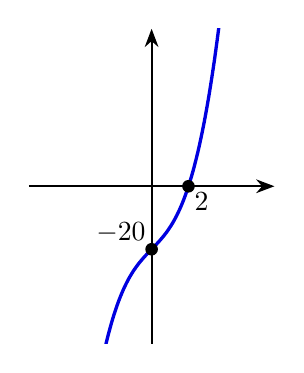
\begin{tikzpicture}
			\begin{scope}[xscale=.78]
				\draw[cstaxis] (-2,0)--(2,0);
				\draw[cstaxis] (0,-2)--(0,2);
				\clip (-2,-2) rectangle (2,2);
				\begin{scope}[xscale=.3,yscale=.04]
					\draw[cstcurve,main,domain=-3:4,smooth] plot (\x,{\x*\x*\x+6*\x-20});
					\coordinate (A) at (2,0);
					\coordinate (B) at (0,-20);
				\end{scope}
				\draw[inner sep=2pt]
					(A) node[below right] {$2$}
					(B) node[above left] {$-20$};
			\end{scope}
			\begin{scope}[cstdot]
				\fill (A) circle;
				\fill (B) circle;
			\end{scope}
		\end{tikzpicture}}
	\end{solution}
\end{frame}


\begin{frame}{三次方程的根\noexer}
	\beqskip{1pt}
	\onslide<+->
	\begin{example}[nearnext]
		解方程 $x^3-7x+6=0$.
	\end{example}
	\onslide<+->
	\begin{solution}[nearprev,sidepic,righthand width=2.7cm,leftupper=0mm]
		\begin{itemize}
			\item 类似地 $x=u+v$, 其中 $u^3+v^3=-6$, $uv=\frac73$.
			\item 于是 $u^3,v^3$ 满足一元二次方程 $X^2+6X+\frac{343}{27}=0$.
			\item 这个方程没有实数解, 我们可以强行解得 
		\end{itemize}
		\onslide<+->{%
		\[
			u^3=-3+\dfrac{10}9\sqrt{-3},\ 
			\visible<+->{u=\frac{3+2\sqrt{-3}}3,\frac{-9+\sqrt{-3}}6,\frac{3-5\sqrt{-3}}6,}
		\]}
		\begin{itemize}
			\item $v=\dfrac{3-2\sqrt{-3}}3,\dfrac{-9-\sqrt{-3}}6,\dfrac{3+5\sqrt{-3}}6$,
			\item $x=u+v=2,-3,1$.
		\end{itemize}
		\tcblower
		\onslide<+->{%
		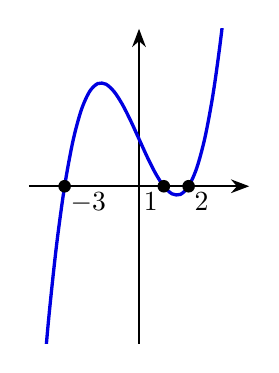
\begin{tikzpicture}
			\begin{scope}[xscale=.7]
				\def\a{-3}
				\def\b{1}
				\def\c{2}
				\draw[cstaxis] (-2,0)--(2,0);
				\draw[cstaxis] (0,-2)--(0,2);
				\clip (-2,-2) rectangle (2,2);
				\begin{scope}[xscale=.45,yscale=.1]
					\draw[cstcurve,main,domain=-4:4,smooth] plot (\x,{(\x-\a)*(\x-\b)*(\x-\c)});
					\coordinate (A) at (\a,0);
					\coordinate (B) at (\b,0);
					\coordinate (C) at (\c,0);
				\end{scope}
				\draw[inner sep=2pt]
					(A) node[below right] {$-3$}
					(B) node[below left] {$1$}
					(C) node[below right] {$2$};
			\end{scope}
			\begin{scope}[cstdot]
				\fill (A) circle;
				\fill (B) circle;
				\fill (C) circle;
			\end{scope}
		\end{tikzpicture}}
	\end{solution}
	\endgroup
\end{frame}


\begin{frame}{三次方程的根\noexer}
	\begin{itemize}
		\item 一般地, 方程 $x^3+px+q=0$ 的解为($p=0$ 情形较简单, 这里不考虑)
		\[
			x=u-\frac p{3u},\quad u^3=-\frac q2+\sqrt{\Delta},\quad \Delta=\frac{q^2}4+\frac{p^3}{27}.
		\]
		\item 通过分析函数图像的极值点可以知道:
	\end{itemize}
	\begin{center}
		\begin{tikzpicture}[visible on=<3->]
			\begin{scope}[scale=.65,
				declare function={
					f(\x)=\x*\x*\x-3*\x;
				}
			]
				\def\a{2.5}
				\draw[cstaxis] (-2,0)--(2,0);
				\draw[cstaxis] (0,-2) node[below] {$\Delta>0$, 有 $1$ 个根}--(0,2);
				\clip (-2,-2) rectangle (2,2);
				\begin{scope}[xscale=.35,yscale=.1]
					\draw[cstcurve,main,domain=-3:4,smooth] plot (\x,{f(\x)-f(\a)});
					\coordinate (A) at (\a,0);
				\end{scope}
			\end{scope}
			\fill[cstdot] (A) circle;
			\begin{scope}[visible on=<4->,xshift=5cm]
				\begin{scope}[scale=.65]
					\def\a{-2}
					\def\b{1}
					\draw[cstaxis] (-2,0)--(2,0);
					\draw[cstaxis] (0,-2) node[below,align=center] {$\Delta=0$, 有 $2$ 个根\\$x=-\sqrt[3]{4q},\half\sqrt[3]{4q}$ ($2$重).}--(0,2);
					\clip (-2,-2) rectangle (2,2);
					\begin{scope}[xscale=.35,yscale=.1]
						\draw[cstcurve,main,domain=-4:3,smooth] plot ({\x},{(\x-\a)*(\x-\b)*(\x-\b)});
						\coordinate (A) at (\a,0);
						\coordinate (B) at (\b,0);
					\end{scope}
				\end{scope}
				\begin{scope}[cstdot]
					\fill (A) circle;
					\fill (B) circle;
				\end{scope}
			\end{scope}
			\begin{scope}[visible on=<5->,xshift=10cm]
				\begin{scope}[scale=.65]
					\def\a{-3}
					\def\b{.5}
					\def\c{2.5}
					\draw[cstaxis] (-2,0)--(2,0);
					\draw[cstaxis] (0,-2) node[below] {$\Delta<0$, 有 $3$ 个根}--(0,2);
					\clip (-2,-2) rectangle (2,2);
					\begin{scope}[xscale=.3,yscale=.05]
						\draw[cstcurve,main,domain=-5:5,smooth] plot ({\x},{(\x-\a)*(\x-\b)*(\x-\c)});
						\coordinate (A) at (\a,0);
						\coordinate (B) at (\b,0);
						\coordinate (C) at (\c,0);
					\end{scope}
				\end{scope}
				\begin{scope}[cstdot]
					\fill (A) circle;
					\fill (B) circle;
					\fill (C) circle;
				\end{scope}
			\end{scope}
		\end{tikzpicture}
	\end{center}
\end{frame}


\begin{frame}{三次方程的根\noexer}
	\begin{itemize}
		\item 由此可见, 若想使用求根公式, 就\alert{必须接受负数开方}.
		\item 那么为什么当 $\Delta<0$ 时, 从求根公式一定能得到 $3$ 个实根呢?
		\item 这个问题在我们学习了第一章的内容之后可以得到回答.
		\item 尽管在十六世纪, 人们已经得到了三次方程的求根公式, 然而对其中出现的虚数, 却是难以接受.
		\item 莱布尼兹曾说: {\color{third}\itshape 圣灵在分析的奇观中找到了超凡的显示, 这就是那个理想世界的端兆, 那个介于存在与不存在之间的两栖物, 那个我们称之为虚的 $-1$ 的平方根。}
		\item 不过, 现在我们可以用更为现代和严格的语言来引入复数.
	\end{itemize}
\end{frame}

\subsection{复数的概念}

\begin{frame}{复数的定义}
	\begin{itemize}
		\item 现在我们来正式介绍复数的概念.
		\item 为了避免记号 $\sqrt{-1}$ 带来的歧义, 我们先引入抽象符号 $\ii$, 再通过定义它的运算来构造复数.
	\end{itemize}
	\onslide<+->
	\begin{definition}
		固定一个记号 $\ii$, \emph{复数}就是形如 $z=x+y\ii$ 的元素, 其中 $x,y$ 均是实数, 且不同的 $(x,y)$ 对应不同的复数.
	\end{definition}
	\begin{itemize}
		\item 实数 $x$ 可以自然地看成复数 $x+0\ii$.
	\end{itemize}
\end{frame}


\begin{frame}{复平面}
	\begin{itemize}
		\item 回忆全体实数、有理数、整数、自然数构成的集合分别记作 $\BR,\BQ,\BZ,\BN$.
		\item 将\emph{全体复数记作 $\BC$}.
		\item 那么 $\BC$ 自然构成一个二维实线性空间, 且 $\{1,\ii\}$ 是一组基. 
		\item 因此它和平面上的点可以建立一一对应, 并将建立起这种对应的平面称为\emph{复平面}.
	\end{itemize}
	\onslide<+->
	\begin{center}
		\begin{tikzpicture}
			\begin{scope}
				\draw[cstaxis] (-.5,0)--(3,0);
				\draw[cstaxis] (0,-.5)--(0,2.5);
				\coordinate [label=below left:$0$] (O) at (0,0);
				\coordinate [label=above:\textcolor{second}{$z=x+y\ii$}] (A) at (2,1.5);
				\coordinate (B) at (2,0);
				\coordinate (C) at (0,1.5);
				\draw[cstdash] (B)--(A)--(C);
				\fill[cstdot,second] (A) circle;
				\draw[third,Latex-Latex,line width=.5mm] (2.8,1)--(4,1) node[midway,below,third] {一一对应};
			\end{scope}
			\begin{scope}[xshift=5cm]
				\coordinate [label=below left:$O$] (O) at (0,0);
				\coordinate [label=above:\textcolor{second}{$Z(x,y)$}] (A) at (2,1.5);
				\coordinate (B) at (2,0);
				\coordinate (C) at (0,1.5);
				\draw[cstdash] (B)--(A)--(C);
				\fill[cstdot,second] (A) circle;
				\draw[decorate,decoration={brace,amplitude=5},main,cstfill1] (O)--(B) node[midway,above=2mm] {$x$};
				\draw[decorate,decoration={brace,amplitude=5},main,cstfill1] (C)--(O) node[midway,right=2mm] {$y$};
				\draw[third,Latex-Latex,line width=.5mm] (2.8,1)--(4,1) node[midway,below,third] {一一对应};
				\draw[cstaxis] (-.5,0)--(3,0);
				\draw[cstaxis] (0,-.5)--(0,2.5);
			\end{scope}
			\begin{scope}[xshift=10cm]
				\draw[cstaxis] (-.5,0)--(3,0);
				\draw[cstaxis] (0,-.5)--(0,2.5);
				\coordinate [label=below left:$O$] (O) at (0,0);
				\coordinate [label=above:\textcolor{second}{$\overrightarrow{OZ}=(x,y)$}] (A) at (2,1.5);
				\draw[cstcurve,cstra,second] (O)--(A);
			\end{scope}
		\end{tikzpicture}
	\end{center}
\end{frame}


\begin{frame}{实部和虚部, 虚数和纯虚数}
	\onslide<+->
	\begin{itemize}
		\item $x,y$ 轴分别对应复平面的\emph{实轴}和\alert{虚轴}.
		\item 称 $z=x+y\ii$ 中 $x=\Re z$ 为 $z$ 的\emph{实部}; $y=\Im z$ 为 $z$ 的\alert{虚部}.
		\item 当虚部 $\Im z=0$ 时, $z$ 为实数, 它落在实轴上.
		\item 不是实数的复数是\textcolor{third}{\bf 虚数}.
		\item 当实部 $\Re z=0$ 且 \alert{$z\neq0$} 时, $z$ 为\alert{纯虚数}, 它落在虚轴上.
	\end{itemize}
	\onslide<1->
	\begin{figure}[hbpt]
		\centering
		\begin{minipage}{.48\textwidth}
			\raggedleft
			\begin{tikzpicture}
				\coordinate [label=below left:$0$] (O) at (0,0);
				\coordinate (B) at (2,0);
				\coordinate (C) at (0,1.5);
				\draw[cstaxis] (-.5,0)--(3,0);
				\draw[cstaxis] (0,-.5)--(0,2.5);
				\begin{scope}[visible on=<3->]
					\draw[decorate,decoration={brace,amplitude=5},main,cstfill1] (B)--(O) node[midway,below=1.5mm] {$\Re z$};
					\draw[decorate,decoration={brace,amplitude=5},second,cstfill2] (C)--(O) node[midway,right=1.5mm] {$\Im z$};
					\coordinate [label=above:\textcolor{third}{$z=x+y\ii$}] (A) at (2,1.5);
					\draw[cstdash] (B)--(A)--(C);
					\fill[cstdot,third] (A) circle;
				\end{scope}
				\begin{scope}[visible on=<2->]
					\coordinate [label=above:\textcolor{main}{实轴}] (R) at (3,0);
					\coordinate [label=right:\textcolor{second}{虚轴}] (I) at (0,2.5);
					\draw[cstaxis,main] (-.5,0)--(R);
					\draw[cstaxis,second] (0,-.5)--(I);
				\end{scope}
				\draw[main,->,thick,visible on=<4->] (-2,.2)-|(.6,0);
				\draw[second,->,thick,visible on=<6->] (-2,1.3)--(0,1.3);
				\draw 
					(-2,.1) node[cstnode,draw=main,text=main,visible on=<4->] {实数}
					(-2,1.2) node[align=center,cstnode,draw=second,text=second,visible on=<6->] {纯虚数\\不含原点};
			\end{tikzpicture}
		\end{minipage}
		\begin{minipage}{.48\textwidth}
			\centering
			\begin{tikzpicture}
				\filldraw[cstcurve,cstfill] (.8,0) circle (2.6 and 2);
				\coordinate (R) at (0,-.8);
				\filldraw[cstcurve,main,fill=white,visible on=<4->] (R) circle (1.2 and .7);
				\coordinate (I) at (0,.8);
				\draw (R) node[align=center,main,visible on=<4->] {实数 \\$0,1,\sqrt2,\pi,\ee$};
				\draw (I) node[align=center,second,visible on=<6->] {纯虚数 \\$\ii,-\ii ,\pi\ii$};
				\draw[cstcurve,second,visible on=<6->] (I) circle (1.2 and .7);
				\draw 
					(3.7,0) node[align=center] {全\\体\\复\\数}
					(2,0) node[align=center,third,visible on=<5->] {虚数 \\$\ii,\pi\ii,\frac{-1+\sqrt 3 \ii}2$};
			\end{tikzpicture}
		\end{minipage}
	\end{figure}
\end{frame}


\begin{frame}{例题:判断实数和纯虚数}
	\onslide<+->
	\begin{example}[nearnext]
		实数 $x$ 取何值时, $z=(x^2+3x-4)+(x^2+5x-6)\ii$ 是:
		\begin{subexample}[2]
			\item 实数;
			\item 纯虚数.
		\end{subexample}
	\end{example}
	\onslide<+->
	\begin{solution}[nearprev]
		\begin{enumerate}
			\item $\Im z=x^2+5x-6=0$, 即 $x=1$ 或 $-6$.
			\item $\Re z=x^2+3x-4=0$, 即 $x=1$ 或 $-4$.
				\onslide<+->{%
					但同时要求 $\Im z=x^2+5x-6\neq 0$, 因此 $x\neq 1$.
				}\onslide<+->{%
					故 $x=-4$.
				}
		\end{enumerate}
	\end{solution}
	\onslide<+->
	\begin{exercise}
		若 $x^2(1+\ii)-x(5+4\ii)+4+3\ii$ 是纯虚数, 则实数 $x=$\fillblankframe{$4$}.
	\end{exercise}
\end{frame}


\subsection{复数的代数运算}


\begin{frame}{复数的加法与减法}
	\begin{itemize}
		\item 设 $z_1=x_1+y_1\ii,z_2=x_2+y_2\ii$.
		\item 定义复数的\emph{加法}和\emph{减法}:
		\[
			z_1+z_2=(x_1+x_2)+(y_1+y_2)\ii,\quad
			z_1-z_2=(x_1-x_2)+(y_1-y_2)\ii.
		\]
		\item 复数的加减法与其对应的向量 $\overrightarrow{OZ}$ 的加减法是一致的.
	\end{itemize}
	\onslide<1->
	\begin{center}
		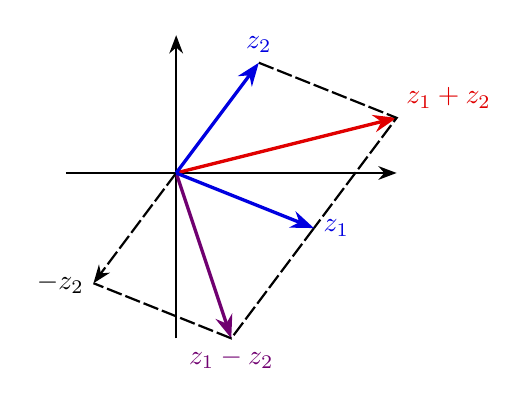
\begin{tikzpicture}[scale=.7]
			\draw[cstaxis] (-2,0)--(4,0);
			\draw[cstaxis] (0,-3)--(0,2.5);
			\coordinate (O) at (0,0);
			\coordinate [label=right:\textcolor{main}{$z_1$}] (Z1) at (2.5,-1);
			\coordinate [label=above:\textcolor{main}{$z_2$}] (Z2) at (1.5,2);
			\begin{scope}[visible on=<3->]
				\coordinate [label=above right:\textcolor{second}{$z_1+z_2$}] (P) at ($(Z1)+(Z2)$);
				\draw[cstcurve,cstra,second] (O)--(P);
				\draw[cstdash] (Z2)--(P)--(Z1);
			\end{scope}
			\begin{scope}[visible on=<4->]
				\coordinate [label=below:\textcolor{third}{$z_1-z_2$}] (M) at ($(Z1)-(Z2)$);
				\coordinate [label=left:{$-z_2$}] (neg) at ($(O)-(Z2)$);
				\draw[cstcurve,cstra,third] (O)--(M);
				\draw[cstdash,cstra] (O)--(neg);
				\draw[cstdash] (Z1)--(M)--(neg);
			\end{scope}
			\draw[cstcurve,cstra,main] (O)--(Z1);
			\draw[cstcurve,cstra,main] (O)--(Z2);
		\end{tikzpicture}
	\end{center}
\end{frame}


\begin{frame}{复数的乘除法}
	\begin{itemize}
		\item \alert{规定 $\ii\cdot \ii=-1$}.
		\item 定义复数的\emph{乘法}:
		\begin{align*}
			z_1\cdot z_2&
			=(x_1+y_1\ii)(x_2+y_2\ii)
			=x_1\cdot x_2+x_1\cdot y_2\ii+y_1\ii\cdot x_2+y_1\ii\cdot y_2\ii\\
			&=(x_1x_2-y_1y_2)+(x_1y_2+x_2y_1)\ii.
		\end{align*}
		\item 此时加法/乘法交换律, 结合律以及乘法分配律均成立.
		\item 待定系数可得复数的\emph{除法}定义为:
		\[
			\frac{z_1}{z_2}
			=\frac{(x_1+y_1\ii)(x_2-y_2\ii)}{x_2^2+y_2^2}
			=\frac{x_1x_2+y_1y_2}{x_2^2+y_2^2}+\frac{x_2y_1-x_1y_2}{x_2^2+y_2^2}\ii.
		\]
		\item 对于正整数 $n$, 定义 $z$ 的 \emph{$n$ 次幂}为 $n$ 个 $z$ 相乘.
		\item 当 $z\neq 0$ 时, 还可以定义 $z^0=1,z^{-n}=\dfrac1{z^n}$.
	\end{itemize}
\end{frame}


\begin{frame}{例: 单位根}
	\onslide<+->
	\begin{example}
		\begin{enumerate}
			\item $\ii^2=-1,\ii^3=-\ii ,\ii^4=1$.
			\onslide<+->{%
			一般地, 对于整数 $n$, 
			\[
				\ii^{4n}=1,\quad \ii^{4n+1}=i,\quad
				\ii^{4n+2}=-1,\quad \ii^{4n+3}=-\ii.
			\]
			}
			\vspace{-\baselineskip}
			\item 令 $\omega=\dfrac{-1+\sqrt 3\ii}2$, 则 $\omega^2=\dfrac{-1-\sqrt3\ii}2,\omega^3=1$.
			\item 令 $z=1+\ii$, \onslide<+->{则
			\[
				z^2=2\ii,\quad z^3=-2+2\ii,\quad z^4=-4,\quad z^8=16=2^4.
			\]}
		\end{enumerate}
		\bigdel\bigdel
	\end{example}
	\begin{itemize}
		\item 将满足 $z^n=1$ 的复数 $z$ 称为 \emph{$n$ 次单位根}.
		\item 那么 $1,\ii,-1,-\ii $ 是 $4$ 次单位根, $1,\omega,\omega^2$ 是 $3$ 次单位根, $-\omega$ 是 $6$ 次单位根.
	\end{itemize}
\end{frame}


\begin{frame}{例: 代数式的计算}
	\begin{itemize}
		\item 实数情形的等差数列求和公式、等比数列求和公式、二项式展开、平方差公式等在复数情形也成立.
	\end{itemize}
	\onslide<+->
	\begin{example}[nearnext]
		化简 $1+\ii+\ii^2+\dots+\ii^{1000}$.
	\end{example}
	\onslide<+->
	\begin{solution}[nearprev]
		根据等比数列求和公式, $1+\ii+\ii^2+\dots+\ii^{1000}
			=\dfrac{\ii^{1001}-1}{\ii-1}
			\visible<+->{=\dfrac{\ii-1}{\ii-1}=1.}$
	\end{solution}
	\onslide<+->
	\begin{exercise}
		化简 $\Bigl(\dfrac{1+\ii}{1-\ii}\Bigr)^{2026}$=\fillblankframe{$-1$}.
	\end{exercise}
\end{frame}


\subsection{共轭复数}


\begin{frame}{共轭复数的定义}
	\onslide<+->
	\begin{definition}
		称 $z$ 在复平面关于实轴的对称点为它的\emph{共轭复数 $\ov z$}.
		换言之, $\ov{x+y\ii}=x-y\ii$.
	\end{definition}
	\onslide<+->
	\begin{exercise}
		$z$ 关于虚轴的对称点是\fillblankframe{$-\ov z$}.
	\end{exercise}
\end{frame}

\begin{frame}{共轭复数的性质}
	\begin{itemize}
		\item 从定义出发, 不难验证共轭复数满足如下性质:
		\begin{enumerate}\bf
			\item $z$ 是 $\ov z$ 的共轭复数.\hfill\alert{共轭是一种对合}
			\item $\ov{z_1\pm z_2}=\ov{z_1}\pm\ov{z_2},\ 
			\ov{z_1\cdot z_2}=\ov{z_1}\cdot\ov{z_2},\ 
			\ov{\Bigl(\dfrac{z_1}{z_2}\Bigr)}=\dfrac{~\ov{z_1}~}{~\ov{z_2}~}$.
			\hfill \alert{共轭复数和四则运算交换}
			\item $z\ov{z}=(\Re z)^2+(\Im z)^2$.
			\item $z+\ov z=2\Re z,\ z-\ov z=2\ii\Im z$.
			\hfill \alert{$x,y$ 和 $z,\ov z$ 可相互表示}
			\item $z=\ov z\iff z$ 是实数; $z=-\ov z\iff z$ 是纯虚数或 $z=0$.\hfill\alert{判断实数和纯虚数}
		\end{enumerate}
		\item 这些性质意味着使用共轭复数进行计算和证明,往往比直接使用 $x,y$ 表达的形式更简单.
	\end{itemize}
\end{frame}


\begin{frame}{例题:共轭复数证明等式}
	\onslide<+->
	\begin{example}
		证明 $z_1\cdot\ov{z_2}-\ov{z_1}\cdot z_2=2\ii\Im(z_1\cdot\ov{z_2})$.
	\end{example}
	\onslide<+->
	我们可以设 $z_1=x_1+y_1\ii,z_2=x_2+y_2\ii$, 然后代入等式两边化简并比较实部和虚部得到.
	\onslide<+->
	但我们利用共轭复数可以更简单地证明它.
	\onslide<+->
	\begin{proof}[leftupper=0mm]
		\begin{itemize}
			\item 由于 $\ov{z_1\cdot\ov{z_2}}=\ov{z_1}\cdot\ov{\ov{z_2}}=\ov{z_1}\cdot z_2$, 
			\item 因此
			\[
				z_1\cdot\ov{z_2}-\ov{z_1}\cdot z_2
				=z_1\cdot\ov{z_2}-\ov{z_1\cdot\ov{z_2}}
				=2\ii\Im(z_1\cdot\ov{z_2}).\qedhere
			\]
		\end{itemize}
	\end{proof}
\end{frame}


\begin{frame}{例题:共轭复数判断实数}
	\onslide<+->
	\begin{example}[nearnext]
		设 $z=x+y\ii$ 是虚数.
		证明: $x^2+y^2=1$ 当且仅当 $z+\dfrac 1z$ 是实数.
	\end{example}
	\onslide<+->
	\begin{proof}[nearprev,leftupper=0mm]
		\begin{itemize}
			\item $z+\dfrac 1z$ 是实数等价于
				$z+\dfrac 1z=\ov{\Bigl(z+\dfrac 1z\Bigr)}=\ov z+\dfrac1{~\ov z~}$,
			\item 等价于
			\[
				z-\ov z=\frac1{~\ov z~}-\frac1z=\frac{z-\ov z}{z\ov z},\quad (z-\ov z)(z\ov z-1)=0.
			\]
			\item 由 $z$ 是虚数可知 $z\neq \ov z$.
			\item 故上述等式等价于 $z\ov z=1$, 即 $x^2+y^2=1$.\qedhere
		\end{itemize}
	\end{proof}
\end{frame}


\begin{frame}{例: 复数的代数计算}
	\onslide<+->
	由于 $z\ov z$ 是一个实数,
	\onslide<+->
	因此在做复数的除法运算时, 可以利用下式将其转化为乘法:
	\[
		\dfrac{z_1}{z_2}=\dfrac{z_1\ov{z_2}}{z_2\ov{z_2}}=\dfrac{z_1\ov{z_2}}{x_2^2+y_2^2}.
	\]
	\bigdel
	\onslide<+->
	\begin{example}[nearnext]
		$z=-\dfrac1\ii-\dfrac{3\ii}{1-\ii }$, 求 $\Re z,\Im z$ 以及 $z\ov z$.
	\end{example}
	\onslide<+->
	\begin{solution}[nearprev]
		\[
			z=-\frac1\ii-\frac{3\ii}{1-\ii }
			\onslide<+->{=\ii-\frac{3\ii-3}2=\frac32-\half \ii,}
		\]
		\onslide<+->{%
		\[
			\Re z=\frac32,\quad\Im z=-\half ,\quad
			z\ov z=\Bigl(\frac32\Bigr)^2+\Bigl(-\half\Bigr)^2=\frac52.
		\]
		}
		\bigdel
	\end{solution}
\end{frame}


\begin{frame}{例: 复数的代数计算}
	\onslide<+->
	\begin{example}[nearnext]
		设 $z_1=5-5\ii,z_2=-3+4\ii$, 求 $\ov{\Bigl(\dfrac{z_1}{z_2}\Bigr)}$.
	\end{example}
	\onslide<+->
	\begin{solution}[nearprev]
		\begin{align*}
			\frac{z_1}{z_2}&=\frac{5-5\ii}{-3+4\ii}
			\onslide<+->{=\frac{(5-5\ii)(-3-4\ii)}{(-3)^2+4^2}}\\
			&\onslide<+->{=\frac{(-15-20)+(-20+15)\ii}{25}}
			\onslide<+->{=-\frac75-\frac15\ii,}
		\end{align*}
		\onslide<+->{%
			因此 $\ov{\Bigl(\dfrac{z_1}{z_2}\Bigr)}=-\dfrac75+\dfrac15\ii$.
		}
	\end{solution}
\end{frame}



% \begin{frame}{复数域\noexer}
% 	\begin{itemize}
% 		\item 复数全体构成一个\emph{域}.
% 		\item 所谓的域, 是指带有如下内容和性质的集合
% 		\begin{itemize}\bf
% 			\item 包含 $0,1$, 且有四则运算;
% 			\item 满足加法结合/交换律, 乘法结合/交换/分配律;
% 			\item 对任意 $a$, $a+0=a\times 1=a$.
% 		\end{itemize}
% 		\item 有理数全体 $\BQ$, 实数全体 $\BR$ 也构成域, 它们是 $\BC$ 的子域.
% 		\item 与有理数域和实数域有着本质不同的是, 复数域是\emph{代数闭域}:
% 		\item 对于任何次数 $n\ge 1$ 的复系数多项式
% 		\[
% 			p(z)=z^n+c_{n-1}z^{n-1}+\cdots+c_1z+c_0,
% 		\]
% 		都存在复数 $z_0$ 使得 $p(z_0)=0$.
% 		\item 由此不难知道, 复系数多项式可以因式分解成一次多项式的乘积.
% 		\item 我们会在第五章证明该结论.
% 	\end{itemize}
% \end{frame}


% \begin{frame}{复数域不是有序域\noexer}
% 	\begin{itemize}
% 		\item \onslide<+->
% 	\end{itemize}
% 	在 $\BQ,\BR$ 上可以定义出一个好的大小关系,
% 	\onslide<+->
% 	换言之它们是有序域, 即存在一个满足下述性质的 $>$:
% 	\begin{itemize}\bf
% 		\item 若 $a\neq b$, 则要么 $a>b$, 要么 $b>a$;
% 		\item 若 $a>b$, 则对于任意 $c$, $a+c>b+c$;
% 		\item 若 $a>b,c>0$, 则 $ac>bc$.
% 	\end{itemize}
% 	\onslide<+->
% 	而 \alert{$\BC$ 却不是有序域}.
% 	\onslide<+->
% 	若 $\ii>0$, 则
% 	\[
% 		-1=\ii\cdot \ii>0,\quad -\ii =-1\cdot \ii>0.
% 	\]
% 	\onslide<+->
% 	于是 $0>\ii$, 矛盾! 同理 $\ii<0$ 也不可能.
% \end{frame}

\section{复数的三角与指数形式}

\subsection{复数的模和辐角}
\begin{frame}{复数的极坐标形式}
	\onslide<+->
	由平面的极坐标表示, 我们可以得到复数的另一种表示方式.
	\onslide<+->
	以 $0$ 为极点, 正实轴为极轴, 逆时针为极角方向可以自然定义出复平面上的极坐标系.
	\onslide<+->
	\begin{center}
		\begin{minipage}{.4\textwidth}
			\centering
			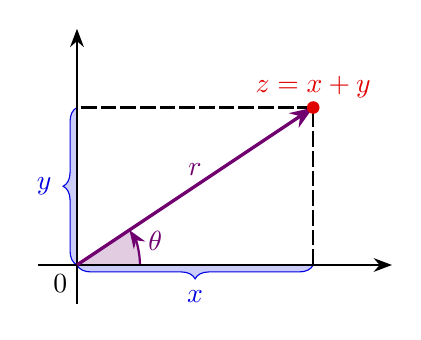
\begin{tikzpicture}
				\coordinate [label=below left:$0$] (O) at (0,0);
				\coordinate [label=above:\textcolor{second}{$z=x+y\ii$}] (Z) at (3,2);
				\coordinate (X) at (3,0);
				\coordinate (Y) at (0,2);
				\draw[decorate,decoration={brace,amplitude=5},main,cstfill1] (X)--(O) node[midway,below=2mm] {$x$};
				\draw[decorate,decoration={brace,amplitude=5},main,cstfill1] (O)--(Y) node[midway,left=2mm] {$y$};
				\draw[third,thick,cstra] pic [cstfill3,draw=third, "$\theta$", angle eccentricity=1.3, angle radius=0.8cm] {angle=X--O--Z};
				\draw[cstaxis] (-.5,0)--(4,0);
				\draw[cstaxis] (0,-.5)--(0,3);
				\draw[cstcurve,third,cstra] (O)--(Z) node[midway,above,third] {$r$};
				\draw[cstdash] (X)--(Z)--(Y);
				\fill[cstdot,second] (Z) circle;
			\end{tikzpicture}
		\end{minipage}
		\begin{minipage}{.56\textwidth}
			\centering
			\onslide<4->{
			\[ x=r\cos\theta,\qquad y=r\sin\theta,
	\]
			\[r=\sqrt{x^2+y^2},\qquad \theta=\arctan\dfrac yx\text{ 或 }\arctan\dfrac yx\pm\pi.\]}
		\end{minipage}
	\end{center}
	\vspace{-\baselineskip}

	\onslide<+->
	\onslide<+->
	\begin{definition}
		\begin{itemize}
			\item 称 $r$ 为 $z$ 的\emph{模}, 记为 \emph{$|z|=r$}.
			\item 称 $\theta$ 为 $z$ 的\emph{辐角}, 记为 \emph{$\Arg z=\theta$}.
			\onslide<+->{约定 \alert{$0$ 的辐角没有定义}.}
		\end{itemize}
	\end{definition}
\end{frame}


\begin{frame}{辐角主值}
	\onslide<+->
	任意 $z\neq 0$ 的辐角有无穷多个.
	\onslide<+->
	我们固定选择其中位于 $(-\pi,\pi]$ 的那个, 并称之为\emph{辐角主值}或\emph{辐角主值}, 记作 $\emphm{\arg z}$.
	\onslide<+->
	那么 $\emphm{\Arg z=\arg z+2k\pi, k\in\BZ}$.

	\onslide<2->
	\begin{figure}[hbpt]
		\centering
		\begin{minipage}{.46\textwidth}
			\onslide<4->{
			\[\arg z=\begin{cases}
				\visible<4->{\emphn{\arctan\dfrac yx,}}&\visible<4->{\emphn{x>0;}}\vspace{1ex}\\
				\visible<5->{\alertn{\arctan\dfrac yx+\pi,}}&\visible<5->{\alertn{x<0,y\ge0;}}\vspace{1ex}\\
				\visible<6->{\color{third}{\arctan\dfrac yx-\pi,}}&\visible<6->{\color{third}{x<0,y<0;}}\\
				\visible<7->{\color{fourth}{\dfrac\pi2,}}&
				\visible<7->{\color{fourth}{x=0,y>0;}}\\
				\visible<7->{\color{fourth}{-\dfrac\pi2,}}&
				\visible<7->{\color{fourth}{x=0,y<0.}}
				\end{cases}\]}
		\end{minipage}
		\begin{minipage}{.52\textwidth}
			\begin{tikzpicture}
				\draw[cstaxis](-2.5,0)->(2.5,0); 
				\draw[cstaxis](0,-2)->(0,2);
				\draw[cstaxis,main,cstwla] (-1.5,0) arc(180:-180:1.5);
				\filldraw[cstdote,draw=main] (-1.5,-.07) circle;
				\begin{scope}[visible on=<4->]
					\coordinate [label=above:\textcolor{main}{$0$}] (A) at (1.7,0);
					\fill[cstdot,main] (A) circle;
					\coordinate [label=above right:\textcolor{main}{$\arctan\dfrac yx$}] (B) at (.9,.9);
					\fill[cstdot,main] (B) circle;
					\coordinate [label=right:\textcolor{main}{$\arctan\dfrac yx$}] (C) at (1.4,-.9);
					\fill[cstdot,main] (C) circle;
				\end{scope}
				\begin{scope}[visible on=<5->]
					\coordinate [label=above left:\textcolor{second}{$\arctan\dfrac yx+\pi$}] (D) at (-1.1,.8);
					\fill[cstdot,second] (D) circle;
					\coordinate [label=below:\textcolor{second}{$\pi$}] (E) at (-.9,0);
					\fill[cstdot,second] (E) circle;
				\end{scope}
				\begin{scope}[visible on=<6->]
					\coordinate [label=left:\textcolor{third}{$\arctan\dfrac yx-\pi$}] (F) at (-1.6,-.7);
					\fill[cstdot,third] (F) circle;
				\end{scope}
				\begin{scope}[visible on=<7->]
					\coordinate [label=left:\textcolor{fourth}{$\dfrac\pi2$}] (G) at (0,.5);
					\fill[cstdot,fourth] (G) circle;
					\coordinate [label=right:\textcolor{fourth}{$-\dfrac\pi2$}] (H) at (0,-.6);
					\fill[cstdot,fourth] (H) circle;
				\end{scope}
			\end{tikzpicture}
		\end{minipage}
	\end{figure}
	\vspace{-\baselineskip}
	\onslide<9->
	注意 \alert{$\arg \ov z=-\arg z$ 未必成立}, 仅当 $z$ 不是负实数和 $0$ 时成立.
\end{frame}


\begin{frame}{复数模的性质}\small
	\onslide<+->
	复数的模满足如下性质:
	\begin{figure}[hbpt]
		\centering
		\begin{minipage}{.48\textwidth}
			\begin{itemize}\bf
				\item $z\ov z=|z|^2=|\ov z|^2$;
				\item $\abs{\Re z},\abs{\Im z}\le |z|\le\abs{\Re z}+\abs{\Im z}$;
			\end{itemize}
		\end{minipage}
		\begin{minipage}{.48\textwidth}
			\begin{itemize}\bf
				\item $\big||z_1|-|z_2|\big|\le|z_1\pm z_2|\le|z_1|+|z_2|$;
				\item $|z_1+z_2+\cdots+z_n|\le|z_1|+|z_2|+\cdots+|z_n|$.
			\end{itemize}
		\end{minipage}
	\end{figure}
	\begin{center}
		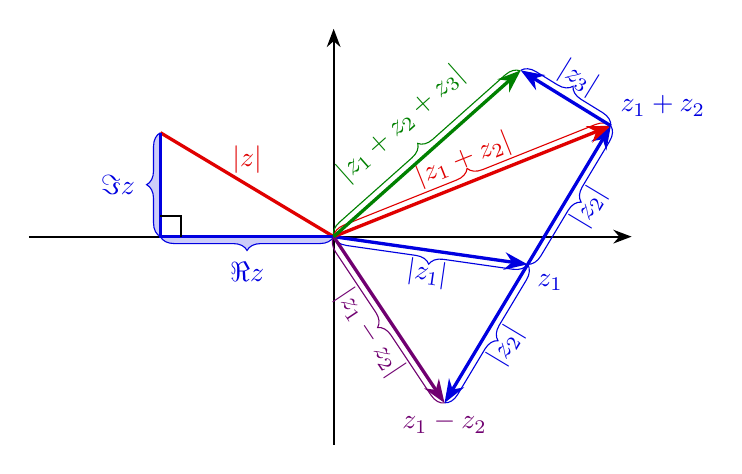
\begin{tikzpicture}[visible on=<3->,scale=.88]
			\draw[cstaxis] (-4.4,0)--(4.3,0);
			\draw[cstaxis] (0,-3)--(0,3);
			\coordinate (O) at (0,0);
			\coordinate (Z) at (-2.5,1.5);
			\coordinate (R) at (-2.5,0);
			\draw[decorate,decoration={brace,amplitude=5},main,cstfill1] (O)--(R) node[midway,below=2mm,main] {$\abs{\Re z}$};
			\draw[decorate,decoration={brace,amplitude=5},main,cstfill1] (R)--(Z) node[midway,left=2mm,main] {$\abs{\Im z}$};
			\draw[cstcurve,second] (O)--(Z) node[midway,above,second] {$|z|$};
			\draw[cstcurve,main] (Z)--(R)--(O);
			\draw[thick] (R) ++(0,.3)--++(.3,0)--++(0,-.3);
	
			\begin{scope}[visible on=<4->]
				\coordinate [label=below right:\textcolor{main}{$z_1$}] (Z1) at (2.8,-.4);
				\coordinate (Z2) at (1.2,2);
				\coordinate [label=above right:\textcolor{main}{$z_1+z_2$}] (P) at ($(Z1)+(Z2)$);
				\coordinate [label=below:\textcolor{third}{$z_1-z_2$}] (M) at ($(Z1)-(Z2)$);
				\draw[decorate,decoration={brace,amplitude=5},main] (Z1)--(O) node[midway,below,sloped] {$|z_1|$};
				\draw[decorate,decoration={brace,amplitude=5},main] (P)--(Z1) node[midway,below,sloped] {$|z_2|$};
				\draw[decorate,decoration={brace,amplitude=5},second] (O)--(P) node[midway,above,sloped] {$|z_1+z_2|$};
				\draw[decorate,decoration={brace,amplitude=5},main] (Z1)--(M) node[midway,below,sloped] {$|z_2|$};
				\draw[decorate,decoration={brace,amplitude=5},third] (M)--(O) node[midway,below,sloped] {$|z_1-z_2|$};
				\begin{scope}[cstcurve,cstra]
					\draw[main] (O)--(Z1);
					\draw[main] (Z1)--(P);
					\draw[second] (O)--(P);
					\draw[third] (O)--(M);
					\draw[main] (Z1)--(M);
				\end{scope}
			\end{scope}

			\begin{scope}[visible on=<5->]
				\coordinate (A) at (2.7,2.4);
				\draw[decorate,decoration={brace,amplitude=5},main] (A)--(P) node[midway,above,sloped] {$|z_3|$};
				\draw[decorate,decoration={brace,amplitude=5},fourth] (O)--(A) node[midway,above=2mm,sloped] {$|z_1+z_2+z_3|$};
				\begin{scope}[cstcurve,cstra]
					\draw[main] (P)--(A);
					\draw[fourth] (O)--(A);
				\end{scope}
			\end{scope}
		\end{tikzpicture}
	\end{center}
\end{frame}


\begin{frame}{例题:共轭复数解决模的等式}
	\beqskip{0pt}
	\onslide<+->
	\begin{example}
		证明
		\begin{enumerate}
			\item $|z_1z_2|=|z_1\ov{z_2}|=|z_1|\cdot|z_2|$;
			\item $|z_1+z_2|^2=|z_1|^2+|z_2|^2+2\Re(z_1\ov{z_2})$.
		\end{enumerate}
	\end{example}

	\onslide<+->
	\begin{proof}
		\begin{enumerate}
			\item 因为
				\[|z_1z_2|^2=z_1z_2\cdot\ov{z_1}\ov{z_2}
				=z_1z_2\ov{z_1}\ov{z_2}=|z_1|^2\cdot|z_2|^2,
	\]
				\onslide<+->{%
					所以 $|z_1z_2|=|z_1|\cdot|z_2|$.
				}\onslide<+->{%
					因此 $|z_1\ov{z_2}|=|z_1|\cdot|\ov{z_2}|=|z_1|\cdot|z_2|$.
				}
			\item 因为
				\begin{align*}
					\text{左边}&=(z_1+z_2)(\ov{z_1}+\ov{z_2})
					=z_1\ov{z_1}+z_2\ov{z_2}+z_1\ov{z_2}+\ov{z_1}z_2,\\
					\text{右边}&=z_1\ov{z_1}+z_2\ov{z_2}+z_1\ov{z_2}+\ov{z_1\ov{z_2}},
				\end{align*}
				\onslide<+->{%
					而 $\ov{z_1\ov{z_2}}=\ov{z_1}z_2$, 所以两侧相等.\qedhere
				}
		\end{enumerate}
	\end{proof}
	\endgroup
\end{frame}


\subsection{复数的三角形式和指数形式}
\begin{frame}{复数的三角形式和指数形式}
	\onslide<+->
	由 $x=r\cos\theta,y=r\sin\theta$ 可得
	\onslide<+->
	\begin{definition}[复数的三角形式]
	\[
		z=r(\cos\theta+\ii\sin\theta).\]	
	\end{definition}
	\onslide<+->
	定义 \alert{$\ee^{\ii\theta}=\exp(\ii\theta):=\cos\theta+\ii\sin\theta$} (欧拉恒等式),
	\onslide<+->
	则我们得到
	\begin{definition}[复数的指数形式]
	\[
		z=r\ee^{\ii\theta}=r\exp(\ii\theta).
	\]
	\end{definition}
	\onslide<+->
	这两种形式的等价的, 指数形式可以认为是三角形式的一种缩写方式.

	\onslide<+->
	求复数的三角和指数形式的\alert{关键在于计算模和辐角}.
\end{frame}


\begin{frame}{例: 求复数的三角和指数形式}
	\onslide<+->
	\begin{example}
		将 $z=-\sqrt{12}-2\ii$ 化成三角形式和指数形式.
	\end{example}

	\onslide<+->
	\begin{solution}
		$r=|z|=\sqrt{12+4}=4$.
		\onslide<+->{%
			由于 $z$ 在第三象限,
		}\onslide<+->{%
			因此
			\[\arg z=\arctan\frac{-2}{-\sqrt{12}}-\pi=\frac\pi6-\pi=-\frac{5\pi}6.
	\]
		}\onslide<+->{%
			故
			\[z=4\left[\cos\Bigl(-\frac{5\pi}6\Bigr)+\ii\sin\Bigl(-
			\frac{5\pi}6\Bigr)\right]=4\ee^{-\frac{5\pi\ii}6}.
	\]
		}
	\end{solution}
\end{frame}


\begin{frame}{例: 求复数的三角和指数形式}
	\beqskip{0pt}
	\onslide<+->
	\begin{example}
		将 $z=\sin\dfrac\pi5+\ii\cos\dfrac\pi5$ 化成三角形式和指数形式.
	\end{example}
	\onslide<+->
	\begin{solution}
		$r=|z|=1$.
		\onslide<+->{%
		由于 $z$ 在第一象限, 因此
		\[\arg z=\arctan\frac{\cos(\pi/5)}{\sin(\pi/5)}=\arctan\cot\frac\pi 5=\frac\pi2-\frac\pi5=\frac{3\pi}{10}.
		\]}\onslide<+->{%
		故
		\[
			z=\cos\frac{3\pi}{10}+\ii\sin\frac{3\pi}{10}=\ee^{\frac{3\pi\ii}{10}}.
		\]}
	\end{solution}
	\onslide<+->
	\begin{solution}[另解]
		\[
			z=\sin\frac\pi5+\ii\cos\frac\pi5
			\visible<+->{=\cos\Bigl(\frac\pi2-\frac\pi5\Bigr)+\ii\sin\Bigl(\frac\pi2-\frac\pi5\Bigr)}
			\visible<+->{=\cos\frac{3\pi}{10}+\ii\sin\frac{3\pi}{10}=\ee^{\frac{3\pi\ii}{10}}.}
		\]
	\end{solution}
	\endgroup
\end{frame}


\begin{frame}{例: 求复数的三角和指数形式}
	\onslide<+->
	求复数的三角或指数形式时, 我们只需要任取一个辐角就可以了, 不要求必须是辐角主值.

	\onslide<+->
	\begin{exercise}
		将 $z=\sqrt 3-3\ii$ 化成三角形式和指数形式.
	\end{exercise}

	\onslide<+->
	\begin{answer}
		$\displaystyle z=2\sqrt3\Bigl(\cos\frac{-\pi}3+\ii\sin\frac{-\pi}3\Bigr)
		=2\sqrt3\ee^{-\frac{\pi\ii}3}$, 写成 $\dfrac{5\pi}3$ 也可以.
	\end{answer}
\end{frame}


\begin{frame}{模为 $1$ 的复数}
	\onslide<+->
	两个模相等的复数之和的三角和指数形式形式较为简单.
	\onslide<+->
	\[
		\ee^{\ii\theta}+\ee^{\ii\varphi}
		=2\cos\frac{\theta-\varphi}2\ee^{\frac{\theta+\varphi}2\ii}.
	\]
	\vspace{-\baselineskip}
	\onslide<+->
	\begin{center}
		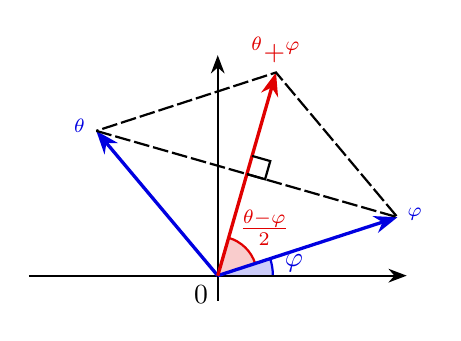
\begin{tikzpicture}[scale=.8]
			\coordinate [label=below left:0] (O) at (0,0);
			\coordinate [label=right:\textcolor{main}{$\ee^{\ii\varphi}$}] (Z1) at ({3*cos(18)},{3*sin(18)});
			\coordinate [label=left:\textcolor{main}{$\ee^{\ii\theta}$}] (Z2) at ({3*cos(130)},{3*sin(130)});
			\coordinate [label=above:\textcolor{second}{$\ee^{\ii\theta}+\ee^{\ii\varphi}$}] (P) at ($(Z1)+(Z2)$);
			\coordinate (M) at ($0.5*(P)$);
			\coordinate (X) at (2,0);
			\draw[thick,main] pic [cstfill1, draw=main,"$\varphi$", angle eccentricity=1.4, angle radius=0.7cm] {angle=X--O--Z1};
			\draw[thick,second] pic [cstfill2, draw=second, "$\frac{\theta-\varphi}2$", angle eccentricity=1.7] {angle=Z1--O--P};
			\draw[cstaxis] (-3,0)--(3,0);
			\draw[cstaxis] (0,-.4)--(0,3.5);
			\draw[cstcurve,cstra,main] (O)--(Z1);
			\draw[cstcurve,cstra,main] (O)--(Z2);
			\draw[cstcurve,cstra,second] (O)--(P);
			\draw[cstdash] (Z2)--(Z1)--(P)--(Z2);
			\draw[thick] (M)--++({.3*cos(16)},{-.3*sin(16)})--++({.3*sin(16)},{.3*cos(16)})--++({-.3*cos(16)},{.3*sin(16)});
		\end{tikzpicture}
	\end{center}
	\onslide<+->
	\begin{example}
		如果 $|z|=1,\arg z=\theta$, 则 $z+1=2\cos\dfrac\theta2 \ee^{\frac{\theta \ii}2}$.
	\end{example}
\end{frame}

\section{方阵的行列式}

\subsection{行列式的定义}

\begin{frame}{引例: 平行四边形的面积\noexer}
	\onslide<+->
	设平面上有 $\parallelogram OACB$, 其中 $A,B$ 坐标分别为 $\bfu=(a,b)^\rmT, \bfv=(c,d)^\rmT$.
\onslide<+->{%
		如果 $\bfu=(1,0)^\rmT,\bfv=(0,1)^\rmT$, 那么面积为 $1$.
	}\onslide<+->{%
		如果将 $\bfu$ 换成 $k\bfu$, 那么面积变为 $|k|$ 倍.
	}\onslide<+->{%
		如果将 $\bfu$ 拆分为 $(a,0)^\rmT+(0,b)^\rmT$, 那么得到的三个平行四边形的面积有什么联系呢?
	}
	\begin{center}
	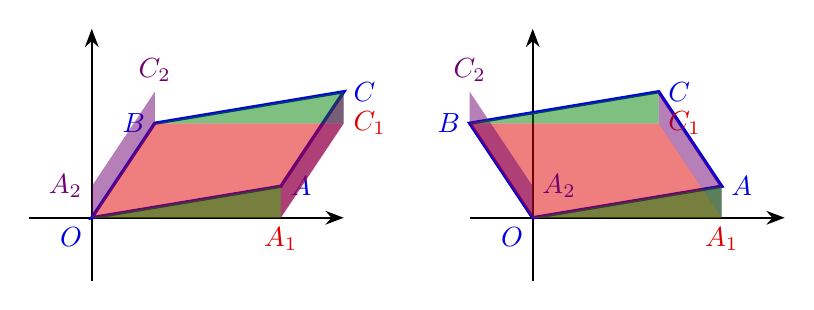
\begin{tikzpicture}[scale=.8]
		\begin{scope}
			\draw[cstaxis] (-1,0)--(4,0);
			\draw[cstaxis] (0,-1)--(0,3);
			\draw[cstcurve,main] (0,0)--(3,0.5)--(4,2)--(1,1.5)--cycle;
			\draw (0,0) node[main,below left] {$O$};
			\draw (3,0.5) node[main,right] {$A$};
			\draw (1,1.5) node[main,left]{$B$};
			\draw (4,2) node[main,right] {$C$};
			\fill[cstcurve,second,fill opacity=.5,visible on=<5->] (0,0)--(3,0)--(4,1.5)--(1,1.5)--cycle;
			\begin{scope}[visible on=<5->]
				\draw (3,0) node[second,below] {$A_1$};
				\draw (4,1.5) node[second,right] {$C_1$};
			\end{scope}
			\fill[cstcurve,third,fill opacity=.5,visible on=<6->] (0,0)--(0,0.5)--(1,2)--(1,1.5)--cycle;
			\begin{scope}[visible on=<6->]
				\draw (0,.5) node[third,left] {$A_2$};
				\draw (1,2) node[third,above] {$C_2$};
			\end{scope}
			\fill[cstcurve,fourth,fill opacity=.5,visible on=<8->] (1,1.5)--(4,1.5)--(4,2)--cycle;
			\fill[cstcurve,fourth,fill opacity=.5,visible on=<9->] (0,0)--(3,0)--(3,0.5)--cycle;
			\fill[cstcurve,third,fill opacity=.5,visible on=<10->] (3,0)--(3,0.5)--(4,2)--(4,1.5)--cycle;
		\end{scope}

		\begin{scope}[xshift=7cm,visible on=<11->]
			\draw[cstaxis] (-1,0)--(4,0);
			\draw[cstaxis] (0,-1)--(0,3);
			\draw[cstcurve,main] (0,0)--(3,0.5)--(2,2)--(-1,1.5)--cycle;
			\draw (0,0) node[main,below left] {$O$};
			\draw (3,0.5) node[main,right] {$A$};
			\draw (-1,1.5) node[main,left]{$B$};
			\draw (2,2) node[main,right] {$C$};
			\fill[cstcurve,second,fill opacity=.5,visible on=<12->] (0,0)--(3,0)--(2,1.5)--(-1,1.5)--cycle;
			\fill[cstcurve,third,fill opacity=.5,visible on=<12->] (0,0)--(0,0.5)--(-1,2)--(-1,1.5)--cycle;
			\begin{scope}[visible on=<12->]
				\draw (3,0) node[second,below] {$A_1$};
				\draw (2,1.5) node[second,right] {$C_1$};
				\draw (0,.5) node[third,right] {$A_2$};
				\draw (-1,2) node[third,above] {$C_2$};
			\end{scope}
			\fill[cstcurve,third,fill opacity=.5,visible on=<13->] (3,0)--(3,0.5)--(2,2)--(2,1.5)--cycle;
			\fill[cstcurve,fourth,fill opacity=.5,visible on=<13->] (0,0)--(3,0)--(3,0.5)--cycle;
			\fill[cstcurve,fourth,fill opacity=.5,visible on=<14->] (-1,1.5)--(2,1.5)--(2,2)--cycle;
		\end{scope}
	\end{tikzpicture}
	\end{center}
	\onslide<+->
	令 $A_1(a,0)$, 并作 $\parallelogram OA_1C_1B$;
	\onslide<+->
	令 $A_2(0,b)$, 并作 $\parallelogram OA_2C_2B$.
	\onslide<+->
	那么 $\parallelogram OACB$ 的面积是这两个相加还是相减?
	\onslide<+->\onslide<+->\onslide<+->
	使用割补法可知为\alert{二者相减}.
	
	\onslide<+->
	如果 $A$ 在第一象限, $B$ 在第二象限.
	\onslide<+->
	那么 $\parallelogram OACB$ 的面积是这两个相加还是相减?\onslide<+->\onslide<+->
	使用割补法可知为\alert{二者相加}.
\end{frame}


\begin{frame}{有向面积\noexer}
	\onslide<+->
	为何第一种情形是相减而第二种情形是相加呢?
	\onslide<+->
	观察发现: 这些平行四边形中只有第一种情形的 $\parallelogram OA_2C_2B$, 从 $OA_2$ 到 $OB$ 是顺时针方向.
	\onslide<+->
	如果定义\emph{有向面积}并记为
	\[|\bfu,\bfv|=\begin{vmatrix}
		a&c\\b&d
	\end{vmatrix}=\begin{cases}
		S_{\parallelogram OACB},&\text{从 $OA$ 到 $OB$ 是逆时针};\\
		-S_{\parallelogram OACB},&\text{从 $OA$ 到 $OB$ 是顺时针}.
	\end{cases}\]
	\onslide<+->
	那么
	\[\begin{vmatrix}
		a&c\\b&d
	\end{vmatrix}=\begin{vmatrix}
		a&c\\0&d
	\end{vmatrix}+\begin{vmatrix}
		0&c\\b&d
	\end{vmatrix}=a\begin{vmatrix}
		1&c\\0&d
	\end{vmatrix}+b\begin{vmatrix}
		0&c\\1&d
	\end{vmatrix}.\]
	\onslide<+->
	换言之, $\bfv$ 固定时, 则 $|\bfu,\bfv|$ 关于 $\bfu$ 是线性的.
	\onslide<+->
	同理, $\bfu$ 固定时, $|\bfu,\bfv|$ 关于 $\bfv$ 也是线性的.
\end{frame}


\begin{frame}{平行多面体情形\noexer}
	\onslide<+->
	将上述概念推广到 $n$ 维情形.
	\onslide<+->
	考虑 $n$ 维空间中由从原点出发的向量 $\bfv_1,\dots,\bfv_n$ 张成的平行多面体.
	\onslide<+->
	如果 $\bfv_1,\dots,\bfv_n$ 就是按顺序各个分量上的单位向量
	\[\bfe_1=(1,0,\dots,0)^\rmT,\quad
	\bfe_2=(0,1,\dots,0)^\rmT,\quad\cdots,\quad
	\bfe_n=(0,0,\dots,1)^\rmT,\]
	则有向面积为 $1$.
	\onslide<+->
	如果交换 $\bfv_i,\bfv_j$ 的位置, 有向面积相差 $-1$ 倍.
	\onslide<+->
	于是得到 $n$ 维情形的有向面积 $|\bfv_1,\dots,\bfv_n|$ 应当满足:
	\begin{enumerate}
		\item $|\bfe_1,\dots,\bfe_n|=1$;
		\item 反对称性: $|\cdots,\bfv_i,\cdots,\bfv_j,\cdots|=-|\cdots,\bfv_j,\cdots,\bfv_i,\cdots|$;
		\item $|\cdots,k\bma,\cdots|=k|\cdots,\bma,\cdots|$;
		\item $|\cdots,\bma+\bmb,\cdots|=|\cdots,\bma,\cdots|+|\cdots,\bmb,\cdots|$.
	\end{enumerate}
\end{frame}


\begin{frame}{行列式的定义\noexer}
	\onslide<+->
	设 $n$ 阶方阵 $\bfA=(a_{ij})$ 的各列形成的向量为 $\bfv_1,\dots,\bfv_n$,
	\onslide<+->
	称有向面积 $|\bfv_1,\cdots,\bfv_n|$ 就是方阵 $\bfA$ 的\emph{行列式}.
	\onslide<+->
	注意到
	\[\bfv_j=a_{1j}\bfe_1+a_{2j}\bfe_2+\cdots+a_{nj}\bfe_n,\]
	\onslide<+->
	利用线性性质将行列式展开将会得到 $n^n$ 项
	\[\sum_{k_1,k_2,\dots,k_n=1}^n|\bfe_{k_1},\cdots,\bfe_{k_n}| a_{k_11}a_{k_22}\cdots a_{k_nn}.\]

	\onslide<+->
	如果 $k_i=k_j$, 则交换 $\bfe_{k_i},\bfe_{k_j}$ 可知 $|\bfe_{k_1},\cdots,\bfe_{k_n}|=0$.
	\onslide<+->
	从而只剩下 $k_1,k_2,\dots,k_n$ 是 $1,2,\dots,n$ 的排列时的那些项.
	\onslide<+->
	例如: 
	\begin{align*}
		\begin{vmatrix}
			a_{11}&a_{12}\\
			a_{21}&a_{22}
		\end{vmatrix}&=|a_{11}\bfe_1,a_{12}\bfe_1+a_{22}\bfe_2|+|a_{21}\bfe_2,a_{12}\bfe_1+a_{22}\bfe_2|\\
		&=a_{11}a_{12}|\bfe_1,\bfe_1|+a_{11}a_{22}|\bfe_1,\bfe_2|+a_{21}a_{12}|\bfe_2,\bfe_1|+a_{21}a_{22}|\bfe_2,\bfe_2|\\
		&=a_{11}a_{22}-a_{21}a_{12}.
	\end{align*}
\end{frame}
	
	
\begin{frame}{行列式的展开形式\noexer}
	\onslide<+->
	设 $k_1,k_2,\dots,k_n$ 是 $1,2,\dots,n$ 的排列.
	\onslide<+->
	如果排列 $k_1,k_2,\dots,k_n$ 需要奇数次对换变成 $1,2,\dots,n$, 记 	$\sgn(k_1,\dots,k_n)=-1$; 否则 $\sgn(k_1,\dots,k_n)=+1$.
	\onslide<+->
	根据反对称性,
	\[|\bfe_{k_1},\cdots,\bfe_{k_n}|=\sgn(k_1,\dots,k_n)|\bfe_1,\cdots,\bfe_n|=\sgn(k_1,\dots,k_n).\]
	\onslide<+->
	\begin{definition}
		设 $\bfA=(a_{ij})$ 是 $n$ 阶方阵.
		定义 $\bfA$ 的\emph{行列式}为
		\[|\bfA|=\sum \sgn(k_1,\dots,k_n) a_{k_11}a_{k_22}\cdots a_{k_nn},\]
		其中 $k_1,k_2,\dots,k_n$ 取遍 $1,2,\dots,n$ 的全体排列.
	\end{definition}
\end{frame}


\begin{frame}{$2,3$ 阶行列式}
	\onslide<+->
	当 $n=2$ 时, $\sgn(12)=1,\sgn(21)=-1$,
	\onslide<+->
	于是
	\[\begin{vNiceMatrix}
		a_{11}&a_{12}\\
		a_{21}&a_{22}
		\CodeAfter
		\tikz \draw[thick,main,visible on=<3->] (1-|1) -- (3-|3);
		\tikz \draw[cstdash,second,visible on=<3->] (3-|1) -- (1-|3);
	\end{vNiceMatrix}
	:=a_{11}a_{22}-a_{12}a_{21}.\]

	\onslide<+->
	\onslide<+->
	当 $n=3$ 时,
	\[\sgn(123)=\sgn(231)=\sgn(312)=1,\]
	\[\sgn(132)=\sgn(213)=\sgn(321)=-1,\]
	\onslide<+->
	于是
	\[\begin{vNiceMatrix}
		a_{11}&a_{12}&a_{13}\\
		a_{21}&a_{22}&a_{23}\\
		a_{31}&a_{32}&a_{33}
		\CodeAfter
		\tikz \draw[thick,main,visible on=<6-8>] (1-|1) -- (4-|4);
		\tikz \draw[thick,second,visible on=<7-8>] (1-|2) -- (3-|4);
		\tikz \draw[thick,second,visible on=<7-8>] (3-|1) -- (4-|2);
		\tikz \draw[thick,third,visible on=<8>] (1-|3) -- (2-|4);
		\tikz \draw[thick,third,visible on=<8>] (2-|1) -- (4-|3);
		\tikz \draw[cstdash,main,visible on=<9->] (1-|4) -- (4-|1);
		\tikz \draw[cstdash,second,visible on=<10->] (1-|3) -- (3-|1);
		\tikz \draw[cstdash,second,visible on=<10->] (3-|4) -- (4-|3);
		\tikz \draw[cstdash,third,visible on=<11->] (1-|2) -- (2-|1);
		\tikz \draw[cstdash,third,visible on=<11->] (2-|4) -- (4-|2);
	\end{vNiceMatrix}
	:=
	a_{11}a_{22}a_{33}+a_{12}a_{23}a_{31}+a_{13}a_{21}a_{32}
	-a_{11}a_{23}a_{32}-a_{12}a_{21}a_{33}-a_{13}a_{22}a_{31}.
	\]
\end{frame}


\begin{frame}{例: $2,3$ 阶行列式的计算}
	\onslide<+->
	\begin{example}
		\begin{align*}
			\begin{vmatrix}
				1&3&2\\3&-5&1\\2&1&4
			\end{vmatrix}
			&\onslide<+->{=1\cdot (-5)\cdot 4+3\cdot 1\cdot2+2\cdot3\cdot1-1\cdot1\cdot1-3\cdot3\cdot4-2\cdot(-5)\cdot2}\\
			&\onslide<+->{=-20+6+6-1-36+20=-25.}
		\end{align*}
	\end{example}
	\onslide<+->
	\begin{exercise}
		若 $k>0$ 且 $\begin{vmatrix}
			k&2&1\\2&k&1\\k&1&2
		\end{vmatrix}=0$, 则 $k=$\fillblankframe{$2$}.
	\end{exercise}
\end{frame}


\begin{frame}{注记}
	\begin{enumerate}
		\item 行列式将一个方阵映射到一个数.
		\item $1$ 阶行列式就是方阵里面唯一的那个元素, 尽管也记作 $|\cdot|$, 但注意和绝对值区分.
		\item $2,3$ 阶行列式可以用对角线法直接得到展开式, 但是更高阶的没有这种表示方法.
		\item \emph{对角阵}的行列式
		\[\bigl|\diag(a_1,a_2,\dots,a_n)\bigr|=a_1a_2\cdots a_n,\]
		特别地 $|\bfE_n|=1,|\bfO_n|=0$.
		\item $|\bfA|$ 是由一些 $\pm a_{k_11}a_{k_22}\cdots a_{k_nn}$ 相加得到, 其中 $k_1,k_2,\dots,k_n$ 取遍 $1,2,\dots,n$ 的所有排列, 一共有 $n!$ 个这样的项, 其中一半取 $+$, 一半取 $-$ ($n\ge2$).
		\item {\itshape $|\bfA|$ 对应的线性变换(常数倍)是 $\bfA$ 对应的线性变换 $\BR^n\ra\BR^n$ 诱导的 $n$ 次外代数上的线性变换 $\bigwedge^n\BR^n\to\bigwedge^n\BR^n$, 感兴趣的可自行阅读有关材料.}
	\end{enumerate}
\end{frame}


% \begin{frame}{三阶行列式的几何意义}
% 	\onslide<+->
% 	类似地, 若 $A(a_1,a_2,a_3),B(b_1,b_2,b_3),C(c_1,c_2,c_3)$,
% 	\onslide<+->
% 	则三阶行列式 $\begin{vmatrix}
% 		a_1&a_2&a_3\\b_1&b_2&b_3\\c_1&c_2&c_3
% 	\end{vmatrix}$ 的绝对值就是下述平行六面体的体积.
% 	\begin{center}
% 	\begin{tikzpicture}[scale=.8]
% 		\draw[cstcurve,main] (0,0)--(3,0)--(4,1.5)--(1,1.5)--cycle;
% 		\draw[cstcurve,main] (4.5,1)--(5.5,2.5)--(2.5,2.5);
% 		\draw[cstdash,cstcurve,main] (2.5,2.5)--(1.5,1)--(4.5,1);
% 		\draw[cstdash,cstcurve,main] (0,0)--(1.5,1);
% 		\draw[cstcurve,main] (3,0)--(4.5,1);
% 		\draw[cstcurve,main] (4,1.5)--(5.5,2.5);
% 		\draw[cstcurve,main] (1,1.5)--(2.5,2.5);
% 		\draw (0,0) node[second,left] {$O$};
% 		\draw (3,0) node[second,right] {$A$};
% 		\draw (1,1.5) node[second,left] {$C$};
% 		\draw (1.5,1) node[second,below] {$B$};
% 	\end{tikzpicture}
% 	\end{center}
% 	\onslide<+->
% 	它的符号则表示使用右手四指从 $OA$ 旋转到 $OB$ 方向时, 大拇指所指方向与 $OC$ 是否在平面 $OAB$ 的同侧.
% \end{frame}


\subsection{行列式的性质}

\begin{frame}{行列式的乘性}
	\onslide<+->
	\begin{theorem@}
		\begin{enumerate}
			\item $|\bfA\bfB|=|\bfA|\cdot|\bfB|$.
		\end{enumerate}
	\end{theorem@}
	\onslide<+->
	\begin{proof}
		设 $f(\bfX):=|\bfA\bfX|$, 即 $f(\bfv_1,\dots,\bfv_n)=|\bfA\bfv_1,\dots,\bfA\bfv_n|$.
	\onslide<+->{%
			容易知道 $f$ 也满足反对称性, 且对任意 $\bfv_i$ 是线性的.
		}\onslide<+->{%
			类似于行列式展开可知, 对于 $\bfX=(a_{ij})$,
			\begin{align*}
				f(\bfX)&=\sum f(\bfe_{k_1},\dots,\bfe_{k_n})a_{k_11}a_{k_22}\cdots a_{k_nn}\\
				&=\sum f(\bfe_1,\dots,\bfe_n)\sgn(k_1,\dots,k_n)a_{k_11}a_{k_22}\cdots a_{k_nn}\\
				&=f(\bfE)|\bfX|=|\bfA|\cdot|\bfX|,
			\end{align*}
			其中 $k_1,k_2,\dots,k_n$ 取遍 $1,2,\dots,n$ 的全体排列.
		}\onslide<+->{%
			故 $|\bfA\bfB|=f(\bfB)=|\bfA|\cdot|\bfB|$.
		}
	\end{proof}
	\onslide<+->
	由此可知, 对于平行多面体 $V\subset \BR^n$, $\bfA$ 对应的线性映射将其面积变为 $|\bfA|$ 倍.
\end{frame}


\begin{frame}{例: 行列式的乘性}
	\onslide<+->
	\begin{example}
		证明:
		$\begin{vmatrix}
			a_1+b_1&b_1+c_1&c_1+a_1\\
			a_2+b_2&b_2+c_2&c_2+a_2\\
			a_3+b_3&b_3+c_3&c_3+a_3
		\end{vmatrix}=2\begin{vmatrix}
			a_1&b_1&c_1\\
			a_2&b_2&c_2\\
			a_3&b_3&c_3
		\end{vmatrix}$.
	\end{example}
	\onslide<+->
	\begin{proof}
		\[\begin{vmatrix}
			a_1+b_1&b_1+c_1&c_1+a_1\\
			a_2+b_2&b_2+c_2&c_2+a_2\\
			a_3+b_3&b_3+c_3&c_3+a_3
		\end{vmatrix}=\begin{vmatrix}
			a_1&b_1&c_1\\
			a_2&b_2&c_2\\
			a_3&b_3&c_3
		\end{vmatrix}\cdot\begin{vmatrix}
			1&0&1\\
			1&1&0\\
			0&1&1
		\end{vmatrix}\onslide<+->{=2\begin{vmatrix}
			a_1&b_1&c_1\\
			a_2&b_2&c_2\\
			a_3&b_3&c_3
		\end{vmatrix}.}\qedhere\]
	\end{proof}
\end{frame}


\begin{frame}{行列式的转置不变性}
	\onslide<+->
	\begin{theorem@}
		\begin{enumerate}
			\setcounter{enumi}{1}
			\item 转置不改变行列式: $|\bfA^\rmT|=|\bfA|$.
		\end{enumerate}
	\end{theorem@}
	\onslide<+->
	一个排列 $k_1,\dots,k_n$ 可以看成是集合 $\{1,2,\dots,n\}$ 到自身的双射 $i\mapsto k_i$.
	\onslide<+->
	设它的逆映射对应的排列是 $\ell_1,\dots,\ell_n$, 则 $\ell_{k_i}=i$.
	\onslide<+->
	由于
	\begin{align*}
		|\bfA|&=\sum\sgn(k_1,\dots,k_n) a_{k_11}\cdots a_{k_nn}=\sum\sgn(k_1,\dots,k_n)a_{1\ell_1}\cdots a_{n\ell_n},\\
		|\bfA^\rmT|&=\sum\sgn(\ell_1,\dots,\ell_n)a_{1\ell_1}\cdots a_{n\ell_n},
	\end{align*}
	\onslide<+->
	我们只需说明 $\sgn(k_1,\dots,k_n)=\sgn(\ell_1,\dots,\ell_n)$.
	\onslide<+->
	设
	\[\bfP=(\bfe_{k_1},\bfe_{k_2},\dots,\bfe_{k_n})\]
	的 $k_i$ 行 $i$ 列为 $1$, 其余项为零.
	\onslide<+->
	那么 $|\bfP|=\sgn(k_1,\dots,k_n)$, $|\bfP^\rmT|=\sgn(\ell_1,\dots,\ell_n)$.
	\onslide<+->
	由于 $\bfP\bfP^\rmT=\bfE$, 因此 $|\bfP|\cdot|\bfP^\rmT|=|\bfE|=1$.
	\onslide<+->
	而 $|\bfP|=\pm1$, 因此 $|\bfP|=|\bfP^\rmT|$.
\end{frame}


\begin{frame}{例: 方阵的行列式}
	\beqskip{6pt}
		\onslide<+->
		\begin{example}
			设 $\bfA=\begin{pmatrix}
				a&-b&-c&-d\\
				b&a&-d&c\\
				c&d&a&-b\\
				d&-c&b&a
			\end{pmatrix}$, 求 $|\bfA|$.
		\end{example}
		\onslide<+->
		\begin{solution}
			这题可以直接硬算, 不过我们可以利用一点小技巧:
		\onslide<+->{%
				\[\bfA\bfA^\rmT=\begin{pmatrix}
					a&-b&-c&-d\\
					b&a&-d&c\\
					c&d&a&-b\\
					d&-c&b&a
				\end{pmatrix}\begin{pmatrix}
					a&b&c&d\\
					-b&a&d&-c\\
					-c&-d&a&b\\
					-d&c&-b&a
				\end{pmatrix}=(a^2+b^2+c^2+d^2)\bfE.\]
			}\onslide<+->{%
				因此 $|\bfA|=\pm(a^2+b^2+c^2+d^2)^2$.
			}\onslide<+->{%
				因为 $|\bfA|$ 一定有 $a^4$ 项, 所以 $|\bfA|=(a^2+b^2+c^2+d^2)^2$.
			}
		\end{solution}
	\endgroup
\end{frame}


\begin{frame}{行列式线性性}
	\onslide<+->
	再根据行列式关于每个列向量的线性性和反对称性有:
	\onslide<+->
	\begin{theorem@}
		\begin{enumerate}
			\setcounter{enumi}{2}
			\item 互换两行(列)后, 方阵的行列式变为 $-1$ 倍.
			\item 方阵的某一行(列)乘 $k$ 后, 方阵的行列式变为 $k$ 倍.
			\item 将方阵某一行(列)对应向量写成两个向量之和, 则行列式也可对应拆成两个行列式之和.
		\end{enumerate}
	\end{theorem@}
	\onslide<+->
	\begin{corollary}
		\begin{enumerate}
			\item 具有相同的两行(列)的方阵的行列式为零: $|\cdots,\bfv,\cdots,\bfv,\cdots|=0$.
			\item 若方阵有一行(列)全为零, 则行列式为零: $|\cdots,{\bf0},\cdots|=0$.
			\item 若方阵有两行(列)成比例, 则行列式为零: $|\cdots,\bfv,\cdots,k\bfv,\cdots|=0$.
			\item 行列式中某一行(列)的公因子可以提到行列式外面.
		\end{enumerate}
	\end{corollary}
\end{frame}


\begin{frame}{初等变换}
	\onslide<+->
	计算行列式可以通过实施下列变换来化简:
	\onslide<+->
	\begin{third}{初等变换}
		\begin{enumerate}
			\item 互换两行(列): $\alertm{r_i\swap r_j, c_i\swap c_j}$, 行列式变号;
			\item 一行(列)乘\alert{非零常数} $k$: $\alertm{kr_i, kc_i}$, 行列式变为 $k$ 倍;
			\item $j$ 行(列)乘 $k$ 加到 $i$ 行(列): $\alertm{r_i+kr_j, c_i+kc_j}$, 行列式不变.
		\end{enumerate}
	\end{third}
	\onslide<+->
	实施第三类初等变换 $c_i+kc_j$ 时, 第 $j$ 列不变, 改变的是第 $i$ 列.
	\onslide<+->
	由于
	\begin{align*}
		|\cdots,\bfv_i,\cdots,\bfv_j,\cdots|
		&=|\cdots,\bfv_i,\cdots,\bfv_j,\cdots|
		+|\cdots,k\bfv_j,\cdots,\bfv_j,\cdots|\\
		&=|\cdots,\bfv_i+k\bfv_j,\cdots,\bfv_j,\cdots|,
	\end{align*}
	\onslide<+->
	因此第三类初等变换不改变行列式的值.
\end{frame}


\begin{frame}{例: 使用初等变换计算行列式}
	\onslide<+->
	\begin{exercise}
		\begin{enumerate}
			\item 判断题: $|\lambda \bfA|=\lambda|\bfA|$. \onslide<+->{\alert{$|\lambda \bfA|=\lambda^n|\bfA|$}}
			\item 判断题: $\begin{vmatrix}
				1&&&\\&2&&\\&&3&\\&&&4
			\end{vmatrix}=-\begin{vmatrix}
				&&&1\\&&2&\\&3&&\\4&&&
			\end{vmatrix}$. \onslide<+->{\alert{$|\bfe_4,\bfe_3,\bfe_2,\bfe_1|=1$}}
			\item 计算 $\begin{vmatrix}
				a_1+b_1&b_1+c_1&c_1+d_1&d_1+a_1\\
				a_2+b_2&b_2+c_2&c_2+d_2&d_2+a_2\\
				a_3+b_3&b_3+c_3&c_3+d_3&d_3+a_3\\
				a_4+b_4&b_4+c_4&c_4+d_4&d_4+a_4
			\end{vmatrix}=$\fillblankframe{$0$}.
			\item 设 $\bfA$ 为 $5$ 阶方阵, $|\bfA|=-1$, 则
				$|2\bfA|=$\fillblankframe{$-32$},
				$\bigl||\bfA|\bfA\bigr|=$\fillblankframe{$1$}.
		\end{enumerate}
	\end{exercise}
\end{frame}


\begin{frame}{例: 方阵的行列式}
	\onslide<+->
	\begin{example}
		计算
		$\begin{vmatrix}
			2\sin a\cos a&\sin a\cos b+\cos a\sin b&\sin a\cos c+\cos a\sin c\\
			\sin b\cos a+\cos b\sin a&2\sin b\cos b&\sin b\cos c+\cos b\sin c\\
			\sin c\cos a+\cos c\sin a&\sin c\cos b+\cos c\sin b&2\sin c\cos c
		\end{vmatrix}$.
	\end{example}
	\onslide<+->
	容易看出该方阵可写成两个方阵之和
	\[\begin{pmatrix}
		\sin a\cos a&\sin a\cos b&\sin a\cos c\\
		\sin b\cos a&\sin b\cos b&\sin b\cos c\\
		\sin c\cos a&\sin c\cos b&\sin c\cos c
	\end{pmatrix}+\begin{pmatrix}
		\cos a\sin a&\cos a\sin b&\cos a\sin c\\
		\cos b\sin a&\cos b\sin b&\cos b\sin c\\
		\cos c\sin a&\cos c\sin b&\cos c\sin c
	\end{pmatrix}.\]
	\onslide<+->
	这两个方阵各自满足各行成比例, 因此可分别写成
	\[\begin{pmatrix}
			\sin a\\
			\sin b\\
			\sin c
		\end{pmatrix}(\cos a,\cos b,\cos c),\qquad
		\begin{pmatrix}
			\cos a\\
			\cos b\\
			\cos c
		\end{pmatrix}(\sin a,\sin b,\sin c).\]
\end{frame}


\begin{frame}{例: 方阵的行列式}
	\onslide<+->
	因此原方阵为
	\[\begin{pmatrix}
			\sin a&\cos a\\
			\sin b&\cos b\\
			\sin c&\cos c
		\end{pmatrix}\cdot\begin{pmatrix}
			\cos a&\cos b&\cos c\\
			\sin a&\sin b&\sin c
		\end{pmatrix}.\]
	\onslide<+->
	\begin{solution}
		原式$=\begin{vmatrix}
			\sin a&\cos a&0\\
			\sin b&\cos b&0\\
			\sin c&\cos c&0
		\end{vmatrix}\cdot\begin{vmatrix}
			\cos a&\cos b&\cos c\\
			\sin a&\sin b&\sin c\\
			0&0&0
		\end{vmatrix}=0$.
	\end{solution}
	\onslide<+->
	设 $\bfA\in M_{m\times n},\bfB\in M_{n\times m}$.
	\onslide<+->
	若 $m>n$, 则
	\[\alertn{|\bfA\bfB|}=\left|
		(\bfA,\bfO_{m\times(m-n)})\begin{pmatrix}
		\bfB\\\bfO_{(m-n)\times m}
	\end{pmatrix}\right|\alertn{=0}.\]
\end{frame}


\begin{frame}{例: 方阵的行列式}
	\onslide<+->
	\begin{example}
		设 $n$ 阶方阵 $\bfA$ 是反对称阵.
		若 $n$ 是奇数, 则 $|\bfA|=0$.
	\end{example}
	\onslide<+->
	\begin{proof}
		由于 $\bfA^\rmT=-\bfA$, 于是
		\[|\bfA|=|\bfA^\rmT|=|{-\bfA}|=(-1)^n|\bfA|=-|\bfA|.\]
	\onslide<+->{%
			故 $|\bfA|=0$.\qedhere
		}
	\end{proof}
\end{frame}


\begin{frame}{例: 使用初等变换计算行列式}\small
	\onslide<+->
	\begin{example}
		若 $abcd=1$, 证明 $\bfA=\begin{pNiceMatrix}
			a^2+a^{-2}&a&a^{-1}&1\\
			b^2+b^{-2}&b&b^{-1}&1\\
			c^2+c^{-2}&c&c^{-1}&1\\
			d^2+d^{-2}&d&d^{-1}&1
		\end{pNiceMatrix}$ 行列式为零.
	\end{example}
	\onslide<+->
	\begin{proof}
		\[|\bfA|=
			\begin{vNiceMatrix}
				a^2&a&a^{-1}&1\\
				b^2&b&b^{-1}&1\\
				c^2&c&c^{-1}&1\\
				d^2&d&d^{-1}&1
			\end{vNiceMatrix}+\begin{vNiceMatrix}
				{a^{-2}}&a&a^{-1}&1\\
				{b^{-2}}&b&b^{-1}&1\\
				{c^{-2}}&c&c^{-1}&1\\
				{d^{-2}}&d&d^{-1}&1
			\end{vNiceMatrix}
			\onslide<+->{=abcd\begin{vNiceMatrix}
				a&1&{a^{-2}}&a^{-1}\\
				b&1&{b^{-2}}&b^{-1}\\
				c&1&{c^{-2}}&c^{-1}\\
				d&1&{d^{-2}}&d^{-1}
			\end{vNiceMatrix}+\begin{vNiceMatrix}
				a&{a^{-2}}&1&a^{-1}\\
				b&{b^{-2}}&1&b^{-1}\\
				c&{c^{-2}}&1&c^{-1}\\
				d&{d^{-2}}&1&d^{-1}
			\end{vNiceMatrix}.}\]
	\onslide<+->{%
			由于 $abcd=1$, 且等式右侧两个行列式相差 $-1$ 倍, 因此 $|\bfA|=0$.\qedhere
		}
	\end{proof}
\end{frame}


\subsection{拉普拉斯展开}

\begin{frame}{余子式和代数余子式}
	\onslide<+->
	我们来介绍行列式与方阵子式的联系.
	\onslide<+->
	\begin{definition}
		设 $\bfA=(a_{ij})$ 是 $n\ge2$ 阶方阵.
		\begin{enumerate}
			\item $\bfA$ 去掉第 $i$ 行和 $j$ 列得到的 $n-1$ 阶方阵的行列式称为 $\bfA$ 在 $(i,j)$ 处的\emph{余子式} (Minor), 记为 $M_{ij}$.
			\item 称 $A_{ij}=(-1)^{i+j}M_{ij}$ 为 $\bfA$ 在 $(i,j)$ 处的\emph{代数余子式} (Algebraic Minor).
		\end{enumerate}
	\end{definition}
	\onslide<+->
	注意余子式和代数余子式是数而不是矩阵.
\end{frame}


\begin{frame}{行列式与余子式的联系\noexer}
	\onslide<+->
	假设 $\bfA$ 的第 $n$ 列除了 $a_{nn}$ 都是零.
	\onslide<+->
	若 $k_n\neq n$, 则 $a_{k_11}\cdots a_{k_nn}=0$; 若 $k_n=n$, 则 $\sgn(k_1,\dots,k_{n-1},n)=\sgn(k_1,\dots,k_{n-1})$.
	\onslide<+->
	因此
	\[|\bfA|=\sum \sgn(k_1,\dots,k_{n-1},n)a_{k_1,1}\cdots a_{k_{n-1},n-1}a_{n,n}=a_{nn} M_{nn}=a_{nn} A_{nn}.\]

	\onslide<+->
	假设 $\bfA$ 的第 $j$ 列除了 $a_{ij}$ 都是零.
	\onslide<+->
	依次对 $\bfA$ 实施
	\[r_i\swap r_{i+1},\quad r_{i+1}\swap r_{i+2},\quad\dots,\quad r_{n-1}\swap r_n,\]
	得到的方阵 $\bfB$ 就是将 $\bfA$ 的第 $i$ 行移动到第 $n$ 行的后面得到的方阵.
	\onslide<+->
	由于一共 $n-i$ 次列互换, 因此 $|\bfB|=(-1)^{n-i}|\bfA|$.

	\onslide<+->
	同理, 将 $\bfB$ 的第 $j$ 列移动到第 $n$ 列的后面得到的方阵记为 $\bfC$, 则
	\[|\bfC|=(-1)^{n-j}|\bfB|=(-1)^{i+j}|\bfA|.\]
	\onslide<+->
	注意到 $\bfC$ 在 $(n,n)$ 处元素是 $a_{ij}$, 余子式是 $M_{ij}$,
	\onslide<+->
	因此
	\[|\bfC|=a_{ij}M_{ij},\qquad |\bfA|=(-1)^{i+j}a_{ij}M_{ij}=a_{ij}A_{ij}.\]
\end{frame}


\begin{frame}{行列式与余子式的联系}
	\onslide<+->
	将 $\bfA$ 的第 $j$ 列写成
	\[\begin{pmatrix}
		a_{1j}\\a_{2j}\\\vdots\\a_{nj}
	\end{pmatrix}
	=\begin{pmatrix}
		a_{1j}\\0\\\vdots\\0
	\end{pmatrix}
	+\begin{pmatrix}
		0\\a_{2j}\\\vdots\\0
	\end{pmatrix}+\cdots+\begin{pmatrix}
		0\\0\\\vdots\\a_{nj}
	\end{pmatrix},\]
	\onslide<+->
	根据行列式的线性性质, 我们得到
	\[|\bfA|=a_{1j}A_{1j}+a_{2j}A_{2j}+\cdots+a_{nj}A_{nj}.\]
	\onslide<+->
	由于转置不改变方阵的行列式, 于是得到
	\[|\bfA|=a_{i1}A_{i1}+a_{i2}A_{i2}+\cdots+a_{in}A_{in}.\]
\end{frame}


\begin{frame}{拉普拉斯展开}
	\onslide<+->
	\begin{second}{行列式沿任一行或列展开}
		方阵的行列式等于任一行(列)的元素与其对应的代数余子式乘积的和:
		\begin{align*}
			|\bfA|&=a_{i1}A_{i1}+a_{i2}A_{i2}+\cdots+a_{in}A_{in}\\
			&=a_{1j}A_{1j}+a_{2j}A_{2j}+\cdots+a_{nj}A_{nj}.
		\end{align*}
	\end{second}
	\onslide<+->
	由此也可以看出 \alert{$i\neq k$ 时,}
	\[\alertn{a_{i1}A_{k1}+a_{i2}A_{k2}+\cdots+a_{in}A_{kn}=0,}\]
	\onslide<+->
	因为它是第 $i,k$ 行相同的方阵的行列式.
\end{frame}


\begin{frame}{例: 三角阵的行列式}
	\onslide<+->
	\begin{example}
		\begin{align*}
			\begin{vmatrix}
				a_{11}&      &      &\\
				a_{21}&a_{22}&      &\\
				\vdots&\vdots&\ddots&\\
				a_{n1}&a_{n2}&\cdots&a_{nn}
			\end{vmatrix}
			&\onslide<+->{=a_{11}\begin{vmatrix}
				a_{22}&      &\\
				\vdots&\ddots&\\
				a_{n2}&\cdots&a_{nn}
			\end{vmatrix}}
			\onslide<+->{=a_{11}a_{22}\begin{vmatrix}
				a_{33}&      &\\
				\vdots&\ddots&\\
				a_{n3}&\cdots&a_{nn}
			\end{vmatrix}}\\
			&\onslide<+->{=\cdots=a_{11}a_{22}\cdots a_{nn}.}
		\end{align*}
		\onslide<+->{
			由于转置不改变行列式, 因此上\alert{三角阵行列式也等于对角元乘积}.}
	\end{example}
\end{frame}


\begin{frame}{例: 反对角阵的行列式}
	\onslide<+->
	\begin{example}
		计算 $|\bfA|$, 其中 $\bfA=\begin{pmatrix}
			&&&a_1\\&&a_2&\\&\udots&&\\a_n&&&
		\end{pmatrix}$.
	\end{example}
	\onslide<+->
	\begin{solution*}
		\begin{align*}
			|\bfA|&=(-1)^{n+1}a_1\begin{vmatrix}
				&&a_2\\&\udots&\\a_n&&
			\end{vmatrix}
			\onslide<+->{=(-1)^{n+1}a_1\cdot (-1)^{n}a_2\begin{vmatrix}
				&&a_3\\&\udots&\\a_n&&
			\end{vmatrix}}\\
			&\onslide<+->{=\cdots=\prod_{i=1}^n (-1)^{n-i}a_i}
			\onslide<+->{=(-1)^{\frac{n(n-1)}2}a_1a_2\cdots a_n.}
		\end{align*}
	\end{solution*}
\end{frame}


\begin{frame}{例: 利用初等变换计算行列式}
	\onslide<+->
	对于具体的方阵, 我们可以利用初等变换将其化为三角阵来计算行列式.
	\onslide<+->
	也可以在某一行或一列只有少数非零元时用拉普拉斯展开来降阶.
	\onslide<+->
	\begin{example}
		\begin{align*}
			\begin{vmatrix}
				2& 3& 1&-1\\
				-4&-5& 1& 3\\
				-3& 1&-5& 3\\
				1&-2& 0&-1
			\end{vmatrix}
			&\onslide<+->{\!\!\xeq[\nsmath{r_1-2r_4}]{\substack{\nsmath{r_2+4r_4}\\\nsmath{r_3+3r_4}}}\!\!
			\begin{vmatrix}
				\alertn0& 7& 1&1\\
				\alertn0&-13& 1&-1\\
				\alertn0&-5&-5&0\\
				\alertn1&-2& 0&-1
			\end{vmatrix}}
			\onslide<+->{=(-1)^{4+1}\begin{vmatrix}
				-13& 1&-1\\
				-5&-5&0\\
					7& 1&1
				\end{vmatrix}}\\
			&\onslide<+->{\xeq{\nsmath{r_3+r_1}}
			-\begin{vmatrix}
				-13& 1&\alertn{-1}\\
				-5&-5&\alertn0\\
				-6& 2&\alertn0
			\end{vmatrix}}
			\onslide<+->{=(-1)^{1+3}\begin{vmatrix}
				-5&-5\\-6&2
			\end{vmatrix}=-40.}
		\end{align*}
	\end{example}
\end{frame}


\begin{frame}{例: 利用初等变换计算行列式}
	\onslide<+->
	\begin{exercise}
		\begin{enumerate}
			\item $\begin{vmatrix}
				-2&0&1\\
				501&200&299\\
				500&200&300
			\end{vmatrix}=$\fillblankframe{$-200$}.
			\item $\begin{vmatrix}
				1&1&1\\
				a&b&c\\
				b+c&c+a&a+b
			\end{vmatrix}=$\fillblankframe{$0$}.
			\item 设 $\bma=(1,0,-1),\bfA=\bma^\rmT\bma$, 则
				$|5\bfE-\bfA^3|=$\fillblankframe{$-75$}.
		\end{enumerate}
	\end{exercise}
	\onslide<+->
	回忆: 若 $\bfA=\bma\bmb^\rmT$, 则 $\bfA^k=\lambda^{k-1}\bfA$, 其中 $k=\bmb^{\rmT}\bma$.
\end{frame}


\begin{frame}{例: 分块矩阵行列式}
	\onslide<+->
	\begin{example}
		设
		\[\bfA=\begin{pmatrix}
			a_{11}&\cdots&a_{1m}\\
			\vdots&\ddots&\vdots\\
			a_{m1}&\cdots&a_{mm}
		\end{pmatrix},\qquad
		\bfB=\begin{pmatrix}
			b_{11}&\cdots&b_{1n}\\
			\vdots&\ddots&\vdots\\
			b_{n1}&\cdots&b_{nn}
		\end{pmatrix},\]
		\[\bfC=\begin{pNiceMatrix}
			a_{11}&\cdots&a_{1m}&&&\\
			\vdots&\ddots&\vdots&&0&\\
			a_{m1}&\cdots&a_{mm}&&&\\
			*&\cdots&*&b_{11}&\cdots&b_{1n}\\
			\vdots&\ddots&\vdots&\vdots&\ddots&\vdots\\
			*&\cdots&*&b_{n1}&\cdots&b_{nn}
			\CodeAfter
			\tikz \draw[cstdash,second] (4-|1) -- (4-|7);
			\tikz \draw[cstdash,second] (1-|4) -- (7-|4);
		\end{pNiceMatrix}.\]
		证明 $|\bfC|=|\bfA|\cdot|\bfB|$.
	\end{example}
\end{frame}


\begin{frame}{例: 分块矩阵行列式}
	\onslide<+->
	\begin{proof*}
		对 $m$ 归纳.
		\onslide<+->{当 $m=1$ 时将 $|\bfC|$ 沿第一行展开可知成立.}

	\onslide<+->{%
			假设命题对于 $m-1$ 成立.
		}\onslide<+->{%
			设 $\bfA$ 在 $(1,j)$ 处的余子式为 $M_{1j}$, $\bfC$ 在 $(1,j)$ 处的余子式为 $N_{1j}$.
		}\onslide<+->{%
			则由归纳假设 $N_{1j}=M_{1j}|\bfB|$.
		}\onslide<+->{%
			因此
			\begin{align*}
				|\bfC|&=\sum_{j=1}^m (-1)^{1+j}a_{1j}N_{1j}\\
				&=\sum_{j=1}^m (-1)^{1+j}a_{1j}M_{1j}|\bfB|
				=|\bfA|\cdot|\bfB|.\qedhere
			\end{align*}
		}
	\end{proof*}
\end{frame}


\begin{frame}{例: 拉普拉斯展开的应用}
	\onslide<+->
	\begin{example}
		设 $\bfA=\begin{pmatrix}
			3&0&4&0\\
			2&2&2&2\\
			0&-7&0&0\\
			5&3&-2&2
		\end{pmatrix}$.
		计算 $A_{41}+A_{42}+A_{43}+A_{44}$ 和 $M_{41}+M_{42}+M_{43}+M_{44}$.
	\end{example}
	\onslide<+->
	\begin{solution}
		由拉普拉斯展开可知
		\[A_{41}+A_{42}+A_{43}+A_{44}
		=\begin{vmatrix}
			3&0&4&0\\
			2&2&2&2\\
			0&-7&0&0\\
			1&1&1&1
		\end{vmatrix}=0.\]
	\end{solution}
\end{frame}


\begin{frame}{例: 拉普拉斯展开的应用}
	\onslide<+->
		\begin{solution}[续解]
			\vspace{-\baselineskip}
			\begin{align*}
				M_{41}+M_{42}+M_{43}+M_{44}
				&=-A_{41}+A_{42}-A_{43}+A_{44}
				=\begin{vmatrix}
					3&0&4&0\\
					2&2&2&2\\
					0&-7&0&0\\
					-1&1&-1&1
				\end{vmatrix}\\
				&\onslide<+->{=7\begin{vmatrix}
					3&4&0\\
					2&2&2\\
					-1&-1&1
				\end{vmatrix}=-28.}
		\end{align*}
	\end{solution}
	\onslide<+->
	\begin{exercise}
		若 $\bfA=\begin{pmatrix}
			a_1&a_2&a_3&f\\
			b_1&b_2&b_3&f\\
			c_1&c_2&c_3&f\\
			d_1&d_2&d_3&f
		\end{pmatrix}$,
		则 $A_{11}+A_{21}+A_{31}+A_{41}=$\fillblankframe{$0$}.
		\vspace{-.2\baselineskip}
	\end{exercise}
\end{frame}


\subsection{行列式的计算举例}


\begin{frame}{例: 行和为常数的行列式}
	\onslide<+->
	计算 $n$ 阶矩阵的行列式可以使用初等变换将其变为三角型, 也可以使用拉普拉斯展开来对其实施降阶.
	\onslide<+->
	\begin{example}
		\begin{align*}
			\begin{vmatrix}
				a&1&\cdots&1\\
				1&a&\cdots&1\\
				\vdots&\vdots&\ddots&\vdots\\
				1&1&\cdots&a
			\end{vmatrix}
		&\onslide<+->{\xeq[\nsmath{i\ge2}]{\nsmath{c_1+c_i}}\begin{vmatrix}
				a+n-1&1&\cdots&1\\
				a+n-1&a&\cdots&1\\
				\vdots&\vdots&\ddots&\vdots\\
				a+n-1&1&\cdots&a
			\end{vmatrix}}
		\onslide<+->{=(a+n-1)\begin{vmatrix}
				1&1&\cdots&1\\
				1&a&\cdots&1\\
				\vdots&\vdots&\ddots&\vdots\\
				1&1&\cdots&a
			\end{vmatrix}}\\
		&\onslide<+->{\xeq[\nsmath{i\ge2}]{\nsmath{r_i-r_1}}(a+n-1)\begin{vmatrix}
				1&1&\cdots&1\\
				0&a-1&\cdots&0\\
				\vdots&\vdots&\ddots&\vdots\\
				0&0&\cdots&a-1
			\end{vmatrix}}
		\onslide<+->{=(a+n-1)(a-1)^{n-1}.}
		\end{align*}
	\end{example}
\end{frame}


\begin{frame}{例: 行和为常数的行列式}
	\onslide<+->
	若方阵的每行(列)之和为常数, 可用此法化简.
	\onslide<+->
	\begin{exercise}
		计算 $n$ 阶行列式 $\begin{vmatrix}
			1+a_1&a_2&\cdots&a_n\\
			a_1&1+a_2&\cdots&a_n\\
			\vdots&\vdots&\ddots&\vdots\\
			a_1&a_2&\cdots&1+a_n
		\end{vmatrix}=$\fillblankframe[4cm]{$1+a_1+\cdots+a_n$}.
	\end{exercise}
\end{frame}


\begin{frame}{例: 箭形行列式}
	\onslide<+->
	\begin{example}
		\[\begin{vmatrix}
			1&1&\cdots&1\\
			1&2&\cdots&0\\
			\vdots&\vdots&\ddots&\vdots\\
			1&0&\cdots&n
		\end{vmatrix}\onslide<+->{\xeq[\nsmath{i\ge 2}]{\nsmath{c_1-\dfrac1i c_i}}
		\begin{vmatrix}
			1-\dfrac12-\cdots-\dfrac1n&1&\cdots&1\\
			0&2&\cdots&0\\
			\vdots&\vdots&\ddots&\vdots\\
			0&0&\cdots&n
		\end{vmatrix}}
		\onslide<+->{=\Bigl(1-\frac12-\cdots-\frac1n\Bigr)n!.}\]
	\end{example}
	\onslide<+->
	一般的箭形行列式均可用此法处理.
\end{frame}


\begin{frame}{例: 特殊形状行列式}\small
	\beqskip{0pt}
	\onslide<+->
	\begin{exercise}
		计算 $n$ 阶行列式 $\begin{vmatrix}
			1&2&3&\cdots&n-1&n\\
			-1&0&3&\cdots&n-1&n\\
			-1&-2&0&\cdots&n-1&n\\
			\vdots&\vdots&\vdots&\ddots&\vdots&\vdots\\
			-1&-2&-3&\cdots&0&n\\
			-1&-2&-3&\cdots&-(n-1)&0
		\end{vmatrix}=$\fillblankframe{$n!$}.
	\end{exercise}
	\onslide<+->
	\begin{answer}
		对该方阵实施 $r_i+r_1,i\ge 2$ 即可化为上三角阵.
	\end{answer}
	\endgroup
\end{frame}


\begin{frame}{例: 降阶法}
	\beqskip{3pt}
	\onslide<+->
	\begin{example}
		计算矩阵 $\bfA_n=\begin{pmatrix}
			   x   &   -1    &    0    &\cdots&   0  &   0  \\
			   0   &    x    &   -1    &\cdots&   0  &   0  \\
			   0   &    0    &    x    &\cdots&   0  &   0  \\
			\vdots &  \vdots & \vdots  &\ddots&\vdots&\vdots\\
			   0   &    0    &    0    &\cdots&   x  &  -1  \\
				a_n  & a_{n-1} & a_{n-2} &\cdots&  a_2 & x+a_1
		\end{pmatrix}$ 的行列式.
	\end{example}
	\onslide<+->
	\begin{solution}
		沿着第一列展开得到
		\[|\bfA_n|=x|\bfA_{n-1}|+(-1)^{1+n}a_n(-1)^{n-1}=x|\bfA_{n-1}|+a_n,\]
	\onslide<+->{%
		递推或归纳可知
		\[|\bfA_n|=x(x|\bfA_{n-2}|+a_{n-1})+a_n=\cdots=x^n+a_1x^{n-1}+a_2x^{n-2}+\cdots+a_n.\]
	}\vspace{-\baselineskip}
	\end{solution}
	\endgroup
\end{frame}

\subsection{三对角和范德蒙型行列式}

\begin{frame}{例: 降阶法计算三对角矩阵行列式}
	\onslide<+->
	\begin{example}
		计算矩阵 $\bfA_n=\begin{pmatrix}
				2  &   1  &   0  &\cdots&   0  &   0  \\
				1  &   2  &   1  &\cdots&   0  &   0  \\
				0  &   1  &   2  &\cdots&   0  &   0  \\
			\vdots&\vdots&\vdots&\ddots&\vdots&\vdots\\
				0  &   0  &   0  &\cdots&   2  &   1  \\
				0  &   0  &   0  &\cdots&   1  &   2  \\
		\end{pmatrix}$ 的行列式.
	\end{example}
\end{frame}


\begin{frame}{例: 降阶法计算三对角矩阵行列式}
	\onslide<+->
	\begin{solution}
		设 $D_n=|\bfA_n|$.
	\onslide<+->{%
		沿着第一行展开得到
		\[|\bfA_n|=2|\bfA_{n-1}|-\begin{vmatrix}
			1  &   1  &   0  &\cdots&   0  &   0  \\
			0  &   2  &   1  &\cdots&   0  &   0  \\
			0  &   1  &   2  &\cdots&   0  &   0  \\
		\vdots&\vdots&\vdots&\ddots&\vdots&\vdots\\
			0  &   0  &   0  &\cdots&   2  &   1  \\
			0  &   0  &   0  &\cdots&   1  &   2
		\end{vmatrix}_{n-1}=2|\bfA_{n-1}|-|\bfA_{n-2}|,\]
	}\onslide<+->{%
		因此
		\[|\bfA_n|-|\bfA_{n-1}|=|\bfA_{n-1}|-|\bfA_{n-2}|=\cdots=|\bfA_2|-|\bfA_1|=1,\]
	}\onslide<+->{%
		从而 $|\bfA_n|=n-1+|\bfA_1|=n+1$.}
	\end{solution}
\end{frame}


\begin{frame}{例: 降阶法计算三对角矩阵行列式}
	\onslide<+->
	若主对角线元素均为 $a$, 上下副对角线元素均为 $b$ 和 $c$, 则
	\[
		|\bfA_n|-a|\bfA_{n-1}|+bc|\bfA_{n-2}|=0.
	\]
	\onslide<+->
	设 $\lambda^2-a\lambda+bc=0$ 的两个根为 $\lambda_1,\lambda_2$, 则归纳可知
	\begin{align*}
		|\bfA_n|&=\lambda_1^n+\lambda_1^{n-1}\lambda_2+\cdots+\lambda_1\lambda_2^{n-1}+\lambda_2^n\\
		&=\begin{cases}
			\dfrac{\lambda_1^{n+1}-\lambda_2^{n+1}}{\lambda_1-\lambda_2},&\text{若}\ \lambda_1\neq \lambda_2;\\[8pt]
			(n+1)\Bigl(\dfrac a2\Bigr)^n,&\text{若}\ \lambda_1=\lambda_2=\dfrac a2.
		\end{cases}
	\end{align*}
\end{frame}


\begin{frame}{例: 范德蒙行列式}
\beqskip{0pt}
	\onslide<+->
	\begin{main}{范德蒙行列式}
		设 $\bfA_n=\begin{pmatrix}
			1&1&1&\cdots&1\\
			x_1&x_2&x_3&\cdots&x_n\\
			x_1^2&x_2^2&x_3^2&\cdots&x_n^2\\
			\vdots&\vdots&\vdots&\ddots&\vdots\\
			x_1^{n-1}&x_2^{n-1}&x_3^{n-1}&\cdots&x_n^{n-1}
		\end{pmatrix}$.
		证明 \alert{$|\bfA_n|=\prod\limits_{1\le i<j\le n}(x_j-x_i)$}.
		\vspace{-.36\baselineskip}
	\end{main}
	\onslide<+->
	\begin{solution}[证明]
		归纳证明.
	\onslide<+->{%
			当 $n=1,2$ 时显然成立.
		}\onslide<+->{%
			设 $n\ge 3$, 由 $r_n-x_1 r_{n-1}, \dots,r_2-x_1r_1$ 得到
			\[|\bfA_n|=\begin{vmatrix}
				1&1&1&\cdots&1\\
				0&x_2-x_1&x_3-x_1&\cdots&x_n-x_1\\
				0&x_2(x_2-x_1)&x_3(x_3-x_1)&\cdots&x_n(x_n-x_1)\\
				\vdots&\vdots&\vdots&\ddots&\vdots\\
				0&x_2^{n-2}(x_2-x_1)&x_3^{n-2}(x_3-x_1)&\cdots&x_n^{n-2}(x_n-x_1)
			\end{vmatrix}.\]}
			\vspace{-.44\baselineskip}
	\end{solution}
\endgroup
\end{frame}


\begin{frame}{例: 范德蒙行列式}
		\onslide<+->
		\begin{proof}[续证]
		\onslide<+->{
			沿着第一列展开, 然后提取每一列的公因式 $(x_j-x_1)$ 得到
		\[|\bfA_n|
		=\prod_{j=2}^n(x_j-x_1)\begin{vmatrix}
				1&1&\cdots&1\\
				x_2&x_3&\cdots&x_n\\
				\vdots&\vdots&\ddots&\vdots\\
				x_2^{n-1}&x_3^{n-1}&\cdots&x_n^{n-1}
			\end{vmatrix}.\]}
			\onslide<+->{由归纳假设可知
			\[|\bfA_n|
		=\prod_{j=2}^n(x_j-x_1)\cdot \prod_{2\le i<j\le n}(x_j-x_i)=\prod_{1\le i<j\le n}(x_j-x_i).\qedhere\]}
	\end{proof}
\end{frame}


\begin{frame}{例: 范德蒙行列式的应用}
	\onslide<+->
	\begin{exercise}
		\begin{enumerate}
			\item $\begin{vmatrix}
				x_1^{-3}&x_2^{-3}&x_3^{-3}&x_4^{-3}\\
				x_1^{-1}&x_2^{-1}&x_3^{-1}&x_4^{-1}\\
				x_1&x_2&x_3&x_4\\
				x_1^{3}&x_2^{3}&x_3^{3}&x_4^{3}
			\end{vmatrix}=$\fillblankframe[6cm][3mm]{\onslide<+->{$x_1^{-3}x_2^{-3}x_3^{-3}x_4^{-3}\prod\limits_{1\le i<j\le 4}(x_j^2-x_i^2)$}}.
			\item $\begin{vmatrix}
				1&1&1&1\\
				1&2&3&4\\
				1&4&9&16\\
				1&8&27&65
			\end{vmatrix}=$\fillblankframe{$14$}.
			\onslide<.->{$\alert{=\begin{vmatrix}
				1&1&1&1\\
				1&2&3&4\\
				1&4&9&16\\
				1&8&27&64
			\end{vmatrix}+\begin{vmatrix}
				1&1&1&1\\
				1&2&3&4\\
				1&4&9&16\\
				0&0&0&1
			\end{vmatrix}}$}
			\item 设 $a,b,c$ 两两不等, 且 $\begin{vmatrix}
				a&b&c\\
				a^2&b^2&c^2\\
				b+c&c+a&a+b
			\end{vmatrix}=0$, 则 $a+b+c=$\fillblankframe{$0$}.
		\end{enumerate}
	\end{exercise}
\end{frame}


\begin{frame}{例: 范德蒙行列式\noexer}
	\onslide<+->
	范德蒙行列式还有另一种证明方式, 这种思路对于其它行列式的计算也有帮助.
	\onslide<+->
	\begin{proof}
		$f=|\bfA_n|$ 是 $x_1,\dots,x_n$ 的多项式, 且次数不超过 $1+2+\cdots+(n-1)$.
	\onslide<+->{%
			由于当 $x_i=x_j$ 时 $f=0$, 因此 $f$ 包含因式 $x_i-x_j$, 从而
			\[f=g\prod_{1\le i<j\le n}(x_j-x_i).\]
		}\onslide<+->{%
			比较两边次数可知 $g$ 是常数.
		}\onslide<+->{%
			注意到 $\prod\limits_{i=1}^n x_i^{i-1}$ 只出现在范德蒙行列式对角元的乘积中, 且它在 $\prod\limits_{1\le i<j\le n}(x_j-x_i)$ 中的系数是 $1$.
		}\onslide<+->{%
			因此 $g=1$.\qedhere
		}
	\end{proof}
\end{frame}


\begin{frame}{特殊形状行列式\noexer}
	% \beqskip{1pt}
	\onslide<+->
	\begin{example}
		计算 $\displaystyle\begin{vmatrix}
			1^{50}&2^{50}&\cdots&100^{50}\\
			2^{50}&3^{50}&\cdots&101^{50}\\
			\vdots&\vdots&\ddots&\vdots\\
			100^{50}&101^{50}&\cdots&199^{50}\\
		\end{vmatrix}$.
	\end{example}
	\onslide<+->
	\begin{proof}
		将第一行换成 $(x+1)^{50},\dots,(x+100)^{50}$, 并将行列式记为 $f(x)$.
	\onslide<+->{%
			那么 $f(1)=\cdots=f(99)=0$.
		}\onslide<+->{%
			注意到 $f$ 的次数不超过 $50$, 因此 $f\equiv 0$.\qedhere
		}
	\end{proof}
	\onslide<+->
	同理若 $k<n-1$, $\Bigl|\bigl((a_i+b_j)^k\bigr)_{1\le i,j\le n}\Bigr|=0$.
	% \onslide<+->
	% 对于 $k=n-1$, 可以通过
	% \[(x+b_j)^k=x^k+\rmC_k^1 x^{k-1} b_j+\cdots+\cdots+b_j^k\]
	% 将这个方阵拆分为
	% \[((a_i+b_j)^{n-1})_{ij}
	% =(a_i^{n-j})_{ij}\cdot \diag(\rmC_{n-1}^0,\rmC_{n-1}^1,\dots,\rmC_{n-1}^{n-1}) \cdot (b_j^{i-1})_{ij}.\]
	% \endgroup
\end{frame}


\begin{frame}{行列式常见计算方法总结}
	\begin{enumerate}
		\item $2,3$ 阶行列式可用对角线法直接展开.
		\item 三角阵行列式等于对角元的乘积, 分块三角阵行列式等于对角阵行列式乘积.
		\item 行列式的计算一般需要用到\alert{三类初等变换}, 创造出足够多的零.
		\item 行列式沿一行(列)的展开往往是\alert{降阶法}的必要手段.
		\item 范德蒙型行列式可处理方阵为元素幂次递增的情形.
	\end{enumerate}
\end{frame}


\section{曲线和区域}


\subsection{复数表平面曲线}


\begin{frame}{例题: 复数方程表圆}
	\onslide<+->
	很多的平面图形能用复数形式的方程来表示.
	\onslide<+->
	这种表示方程有些时候会显得更加直观和易于理解.
	\onslide<+->
	\begin{example}[sidepic,righthand width=3.3cm,indent]
		$\abs{z+2\ii}=2$.
		\onslide<+->{%
			该方程表示与 $-2\ii $ 的距离为 $2$ 的点全体, 即圆心为 $-2\ii $ 半径为 $2$ 的圆.
		}
		
		\onslide<+->{%
			一般的圆方程为 $\abs{z-z_0}=R$, 其中 $z_0$ 是圆心, $R$ 是半径.
		}
		\tcblower
		\onslide<4->{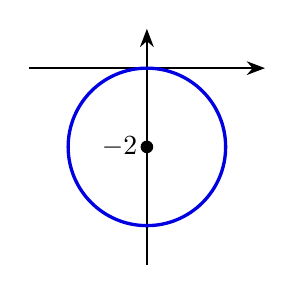
\begin{tikzpicture}
			\draw[cstaxis] (-1.5,0)--(1.5,0);
			\draw[cstaxis] (0,-2.5)--(0,.5);
			\coordinate (A) at (0,-1);
			\fill[cstdot] (A) circle
				node[left] {$-2\ii $};
			\draw[cstcurve,main] (A) circle (1);
		\end{tikzpicture}}
	\end{example}
\end{frame}


\begin{frame}{例题: 复数方程表直线}
	\onslide<+->
	\begin{example}[sidepic,righthand width=3.3cm]
		$\abs{z-4\ii}=\abs{z-2}$.
		\onslide<+->{%
			该方程表示与 $4\ii$ 和 $2$ 的距离相等的点, 即二者连线的垂直平分线.
		}\onslide<+->{%
			两边同时平方化简可得 $x-2y+3=0$.
		}\onslide<+->{%
			该方程也可以表达为
			\[
				(1+2\ii)z+(1-2\ii)\ov z+6=0.
			\]
		}
		\tcblower
		\onslide<2->{
      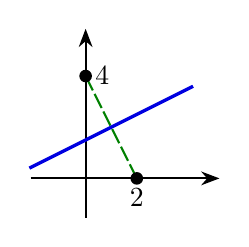
\begin{tikzpicture}[
        declare function={
          f(\y)=2*\y-1.5;
        }
      ]
        \def\u{.65}
        \draw[cstaxis] (-.7,0)--(1.7,0);
        \draw[cstaxis] (0,-.5)--(0,1.9);
        \coordinate (A) at (\u,0);
        \coordinate (B) at (0,{2*\u});
        \draw[cstdash,fourth] (A)--(B);
        \draw[cstcurve,main] ({f(.2)*\u},{.2*\u})--({f(1.8)*\u},{1.8*\u});
        \begin{scope}[cstdot]
          \fill (A) circle node[below] {$2$};
          \fill (B) circle node[right] {$4\ii$};
        \end{scope}
      \end{tikzpicture}}
	\end{example}
\end{frame}


\begin{frame}{例题: 复数方程表椭圆和双曲线}
	\onslide<+->
	\begin{example}
		$\abs{z-z_1}+\abs{z-z_2}=2a$.
		\begin{itemize}
			\item 当 $2a>\abs{z_1-z_2}$ 时, 该方程表示以 $z_1,z_2$ 为焦点, $a$ 为长半轴的椭圆;
			\item 当 $2a=\abs{z_1-z_2}$ 时, 该方程表示连接 $z_1,z_2$ 的线段;
			\item 当 $2a<\abs{z_1-z_2}$ 时, 该方程表示空集.
		\end{itemize}
	\end{example}
	\onslide<+->
	\begin{example}
		$\abs{z-z_1}-\abs{z-z_2}=2a$.
		\begin{itemize}
			\item 当 $2a<\abs{z_1-z_2}$ 时, 该方程表示以 $z_1,z_2$ 为焦点, $a$ 为实半轴的双曲线的一支;
			\item 当 $2a=\abs{z_1-z_2}$ 时, 该方程表示以 $z_2$ 为起点, 与 $z_2,z_1$ 连线反向的射线;
			\item 当 $2a>\abs{z_1-z_2}$ 时, 该方程表示空集.	
		\end{itemize}
	\end{example}
\end{frame}


\begin{frame}{例题: 复数方程表平面图形}
	\onslide<+->
	\begin{exercise}[nearnext]
		$z^2+\ov z^2=1$ 和 $z^2-\ov z^2=\ii$ 分别表示什么图形?
	\end{exercise}

	\onslide<+->
	\begin{answer}[nearprev]
		双曲线 $x^2-y^2=\dfrac12$ 和双曲线 $xy=\dfrac14$.
	\end{answer}
\end{frame}


\begin{frame}{连续曲线、闭路}
	\onslide<+->
	设 $x(t),y(t),t\in[a,b]$ 是两个连续函数.
	\onslide<+->
	参变量方程 $\begin{cases}
		x=x(t),& \\y=y(t),&
	\end{cases}t\in[a,b]$ 定义了一条\emph{连续曲线}.
	\onslide<+->
	这也等价于 $C:z=z(t)=x(t)+\ii y(t),t\in[a,b]$.
	\begin{itemize}
		\item 若除了两个端点有可能重叠外, 其它情形不会出现重叠的点, 则称 $C$ 是\emph{简单曲线}.
		\item 若连续曲线 $C$ 满足两个端点重叠, 即 $z(a) = z(b)$, 则称 $C$ 是闭合曲线.
		\item 称闭合的简单曲线为\emph{简单闭曲线}或\emph{闭路}.
	\end{itemize}
	\onslide<3->
	\begin{center}
		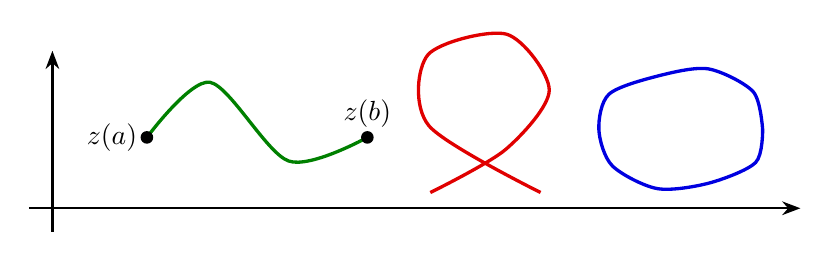
\begin{tikzpicture}
			\draw[cstaxis](-.3,.5)--(9.5,.5);
			\draw[cstaxis](0,.2)--(0,2.5);
			\coordinate (A) at (1.2,1.4);
			\coordinate (B) at (4,1.4);
			\draw[cstcurve,fourth,smooth] plot coordinates {(A) (2,2.1) (3,1.1) (B)};
			\fill[cstdot] (A) circle node[left] {$z(a)$};
			\fill[cstdot] (B) circle node[above] {$z(b)$};
			\draw[cstcurve,second,smooth,visible on=<4->] plot coordinates {(4.8,.7) (5.76,1.25) (6.31,2) (5.77,2.71) (4.77,2.45) (4.78,1.55) (6.2,.7) };
			\draw[cstcurve,main,smooth,visible on=<5->] plot coordinates {(9.02,1.5) (8.9,1.98) (8.33,2.27) (7.69,2.18) (7.07,1.95) (6.94,1.5) (7.11,1.04) (7.68,.75) (8.34,.82) (8.93,1.08) (9.02,1.5)};
		\end{tikzpicture}
	\end{center}
\end{frame}


\begin{frame}{例题: 连续曲线}
	\onslide<+->
	\begin{example}[near]
		圆 $\abs{z-z_0}=R$ 的参数方程: $z=z_0+R\ee^{\ii\theta},\quad\theta\in[0,2\pi]$.
	\end{example}
	\onslide<+->
	\begin{example}[sidepic,righthand width=150pt,near]
		直线段:
		\[
			z(t)=z_0+(z_1-z_0)t,\quad t\in[0,1],
		\]
		其中 $z_0,z_1$ 为两个端点.
		它是简单曲线.
		\tcblower
		\begin{center}
			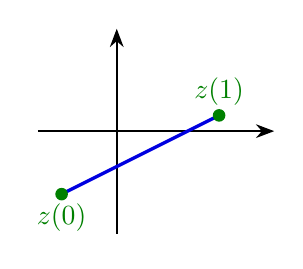
\begin{tikzpicture}
				\draw[cstaxis] (-1.3,.3)--(1.7,.3);
				\draw[cstaxis] (-.3,-1)--(-.3,1.6);
				\coordinate (A) at (-1,-.5);
				\coordinate (B) at (1,.5);
				\draw[cstcurve,main] (A)--(B);
				\begin{scope}[cstdot,fourth]
					\fill (A) circle node[below] {$z(0)$};
					\fill (B) circle node[above] {$z(1)$};
				\end{scope}
			\end{tikzpicture}
		\end{center}
	\end{example}
	\onslide<+->
	\begin{example}[sidepic,righthand width=150pt,near]
		正弦函数曲线段
		\[
			z(t)=\sin t,\quad t\in[0,2\pi]
		\]
		是简单曲线.
		\tcblower
		\begin{center}
			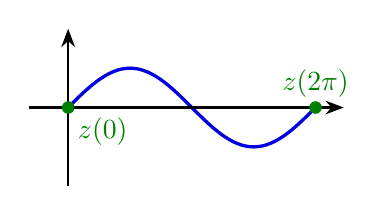
\begin{tikzpicture}
				\draw[cstcurve,main,domain=0:360,smooth] plot ({\x*pi/360},{sin(\x)*.5});
				\draw[cstaxis] (0,-1)--(0,1);
				\draw[cstaxis] (-.5,0)--(3.5,0);
				\coordinate (C) at (0,0);
				\coordinate (D) at ({pi},0);
				\begin{scope}[cstdot,fourth]
					\fill (C) circle node[below right] {$z(0)$};
					\fill (D) circle node[above] {$z(2\pi)$};
				\end{scope}
			\end{tikzpicture}
		\end{center}
	\end{example}
\end{frame}


\begin{frame}{例题: 连续曲线}
	\onslide<+->
	\begin{example}[sidepic,righthand width=150pt]
		椭圆 $\abs{z-\sqrt5}+\abs{z+\sqrt5}=6$ 的参数方程: 
		\[
			z=3\cos\theta+2\ii\sin\theta,\quad \theta\in[0,2\pi].
		\]
		\tcblower
		\begin{center}
			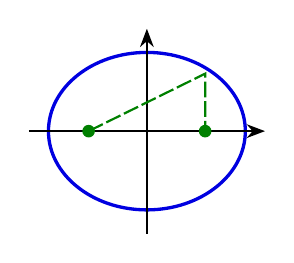
\begin{tikzpicture}
				\coordinate (E) at (-.74,0);
				\coordinate (F) at (.74,0);
				\draw[cstcurve,main] (0,0) circle(1.25 and 1);
				\draw[cstaxis] (-1.5,0)--(1.5,0);
				\draw[cstaxis] (0,-1.3)--(0,1.3);
				\draw[cstdash,fourth] (E)--(.74,.73)--(F);
				\begin{scope}[cstdot,fourth]
					\fill (E) circle;
					\fill (F) circle;
				\end{scope}
			\end{tikzpicture}
		\end{center}
	\end{example}
	\onslide<+->
	\begin{example}[sidepic,righthand width=150pt]
		双纽线 $\abs{z^2-1}=1$ 是闭合曲线, 但不是闭路.
		\tcblower
		\begin{center}
			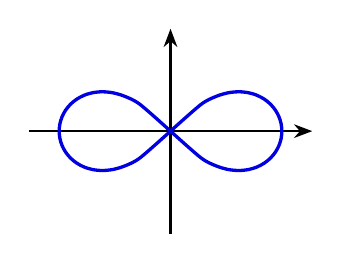
\begin{tikzpicture}
				\draw[cstaxis] (-1.8,0)--(1.8,0);
				\draw[cstaxis] (0,-1.3)--(0,1.3);
				\draw[cstcurve,main,domain=-45:45,smooth] plot ({sqrt(2*cos(2*\x))*cos(\x)},{sqrt(2*cos(2*\x))*sin(\x)});
				\draw[cstcurve,main,domain=-45:45,smooth] plot ({-sqrt(2*cos(2*\x))*cos(\x)},{sqrt(2*cos(2*\x))*sin(\x)});
			\end{tikzpicture}
		\end{center}
	\end{example}
\end{frame}


\subsection{区域和闭区域}


\begin{frame}{邻域}
	\onslide<+->
	为了引入极限的概念, 我们需要考虑点的邻域.
	\onslide<+->
	类比于高等数学中的邻域和去心邻域, 我们在复变函数中, 称开圆盘
		\[
			U(z_0,\delta)=\{z:\abs{z-z_0}<\delta\}
		\]
		为 $z_0$ 的一个 \emph{$\delta$-邻域}.
	\onslide<+->
	称去心开圆盘
		\[
			\Uc(z_0,\delta)=\{z:0<\abs{z-z_0}<\delta\}
		\]
		为 $z_0$ 的一个\emph{去心 $\delta$-邻域}.
	\onslide<2->
	\begin{center}
		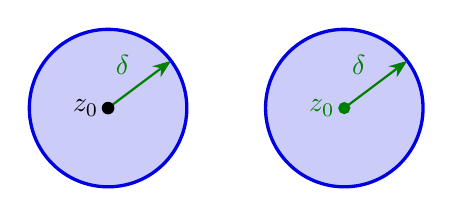
\begin{tikzpicture}
			\begin{scope}
				\coordinate (A) at (-1,0);
				\coordinate (B) at (2,0);
				\filldraw[cstcurve,main,cstfill1] (A) circle (1);
				\filldraw[cstcurve,main,cstfill1,visible on=<3->] (B) circle (1);
				\draw[cstra,fourth,thick] (A)--++(.8,.6)
					node[midway,above left] {$\delta$};
				\draw[cstra,fourth,thick,visible on=<3->] (B)--++(.8,.6)
					node[midway,above left] {$\delta$};
			\end{scope}
			\fill[cstdot] (A) circle node[left] {$z_0$};
			\filldraw[cstdote,fourth,visible on=<3->] (B) circle node[left] {$z_0$};
		\end{tikzpicture}
	\end{center}
\end{frame}


\begin{frame}{内部、外部、边界}
	\onslide<+->
	设 $G$ 是复平面的一个子集, $z_0\in\BC$.
	\onslide<+->
	它们的位置关系有三种可能:
		\begin{enumerate}
			\item 若存在 $z_0$ 的一个邻域 $U$ 完全包含在 $G$ 中, 则称 $z_0$ 是 $G$ 的一个\emph{内点}.
			\item 若存在 $z_0$ 的一个邻域 $U$ 完全不包含在 $G$ 中, 则称 $z_0$ 是 $G$ 的一个\emph{外点}.
			\item 若 $z_0$ 既不是内点也不是外点, 则称 $z_0$ 是 $G$ 的一个\emph{边界点}.
		\end{enumerate}
	\onslide<+->
	内点都属于 $G$, 外点都不属于 $G$, 而边界点则都有可能.
	\onslide<+->
	这类比于区间的端点和区间的关系.
	\onslide<1->
	\begin{center}
		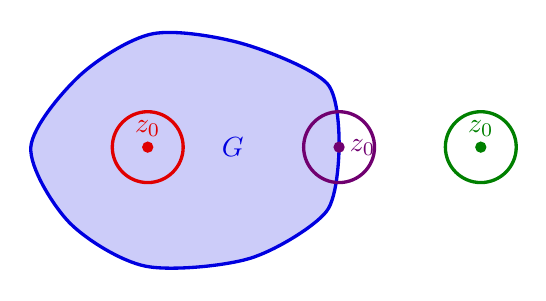
\begin{tikzpicture}[scale=.9]
			\filldraw[cstcurve,main,cstfill1,smooth] plot coordinates {(2,0) (1.83,.9) (.64,1.46) (-.63,1.6) (-1.66,1.01) (-2.35,0) (-1.81,-1.06) (-.73,-1.68) (.74,-1.57) (1.82,-.91) (2,0)};
			\begin{scope}[visible on=<3->]
				\coordinate (A) at (-.7,0);
				\draw[cstcurve,second] (A) circle (.5) node[above] {$z_0$};
				\fill[cstdot,second] (A) circle;
			\end{scope}
			\begin{scope}[visible on=<5->]
				\coordinate (B) at (2,0);
				\draw[cstcurve,third] (B) circle (.5) node[right] {$z_0$};
				\fill[cstdot,third] (B) circle;
			\end{scope}
			\begin{scope}[visible on=<4->]
				\coordinate (C) at (4,0);
				\draw[cstcurve,fourth] (C) circle (.5) node[above] {$z_0$};
				\fill[cstdot,fourth] (C) circle;
			\end{scope}
			\draw (.5,0) node[main] {$G$};
		\end{tikzpicture}
	\end{center}
\end{frame}


\begin{frame}{开集和闭集、有界和无界}
	\onslide<+->
	\begin{definition}[nearnext]
		\begin{enumerate}
			\item 若 $G$ 的所有点都是内点, 也就是说, $G$ 的边界点都不属于它, 称 $G$ 是一个\emph{开集}.
			\item 若 $G$ 的所有边界点都属于 $G$, 称 $G$ 是一个\emph{闭集}.
		\end{enumerate}
	\end{definition}
	\onslide<+->
	$G$ 是一个闭集当且仅当它的补集是开集.

	\onslide<+->
	例如
	\[
		\abs{z-z_0}<R,\quad 1<\Re z<3,\quad\frac\pi4<\arg z<\dfrac{3\pi}4
	\]
	都是开集.
	\onslide<+->
	直观上看: 开集往往由 $>,<$ 的不等式给出, 闭集往往由 $\ge,\le$ 的不等式给出. 
	\onslide<+->
	不过注意这并不是绝对的.

	\onslide<+->
	若 $D$ 可以被包含在某个开圆盘 $U(0,R)$ 中, 则称它是\emph{有界}的.
	\onslide<+->
	否则称它是\emph{无界}的.
\end{frame}


\begin{frame}{区域和闭区域}
	\onslide<+->
	\begin{definition}
		若开集 $D$ 的任意两个点之间都可以用一条完全包含在 $D$ 中的折线连接起来, 则称 $D$ 是一个\emph{区域}.
		\onslide<+->{%
			也就是说, 区域是连通的开集.
		}
	\end{definition}
	\onslide<+->
	\begin{twopart}[indent]{132pt}
		观察右侧图案, 阴影部分(不包含线条部分)中任意两点可用折线连接, 因此它是一个区域.
		\onslide<+->
		这些线条和点构成了它的边界.

		\onslide<+->
		区域和它的边界一起构成了\emph{闭区域}, 记作 $\ov D$.
		\onslide<+->
		它是一个闭集.
		\tcblower
		\onslide<3->
		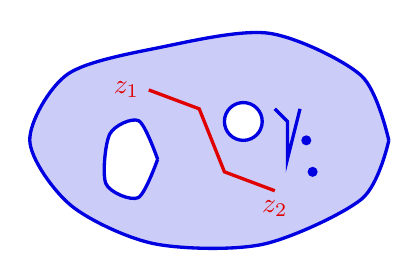
\begin{tikzpicture}[scale=.8]
			\filldraw[cstcurve,main,cstfill1,smooth] plot coordinates {(2.81,0) (2.37,1.03) (.91,1.7) (-.8,1.48) (-2.29,1.05) (-2.89,0) (-2.24,-1.03) (-.92,-1.64) (.81,-1.65) (2.38,-.93) (2.81,0)};
			\filldraw[cstcurve,main,fill=white,smooth] plot coordinates {(-.86,-.3) (-1.16,.31) (-1.62,.1) (-1.68,-.69) (-1.17,-.91) (-.86,-.3)};
			\filldraw[cstcurve,main,fill=white] (.5,.3) circle (.3);
			\fill[cstdot,main] (1.5,0) circle;
			\fill[cstdot,main] (1.6,-.5) circle;
			\draw[cstcurve,second,main] plot coordinates {(1,.5) (1.2,.3) (1.2,-.3) (1.4,.5)};
			\coordinate [label=left:\textcolor{second}{$z_1$}] (A) at (-1,.8);
			\coordinate [label=below:\textcolor{second}{$z_2$}] (B) at (1,-.8);
			\draw[cstcurve,second] (A)--(-.2,.5)--(.2,-.5)--(B);
		\end{tikzpicture}
	\end{twopart}
	\onslide<+->
	注意数学中边界的概念与日常所说的边界是两码事.
	\onslide<+->
	例如区域 $\abs{z}>1$ 的边界是 $\abs{z}=1$, 其闭区域是 $\abs{z}\ge 1$.
\end{frame}


\begin{frame}{常见区域}\small
	\onslide<+->
	很多区域可以由复数的实部、虚部、模和辐角的不等式所确定.
	\onslide<7->{%
		下方区域对应的闭区域是什么?
	}\bigdel
	\onslide<2->
	\begin{figure}[hbpt]
		\begin{minipage}{.24\textwidth}
			\centering
			\begin{tikzpicture}[scale=.7]
				\draw[cstaxis](-1.5,0)--(1.5,0);
				\draw[cstaxis](0,-1.5)--(0,1.5);
				\fill[cstfille1] (-1.2,0) rectangle (1.2,.8);
				\draw (0,-1.5) node[below,align=center] {上半平面\\$\Im z>0$};
			\end{tikzpicture}
		\end{minipage}
		\begin{minipage}{.24\textwidth}
			\centering
			\begin{tikzpicture}[scale=.7]
				\draw[cstaxis](-1.5,0)--(1.5,0);
				\draw[cstaxis](0,-1.5)--(0,1.5);
				\fill[cstfille1] (-1.2,0) rectangle (1.2,-.8);
				\draw (0,-1.5) node[below,align=center] {下半平面\\$\Im z<0$};
			\end{tikzpicture}
		\end{minipage}
		\begin{minipage}{.24\textwidth}
			\centering
			\begin{tikzpicture}[scale=.7,visible on=<3->]
				\draw[cstaxis](-1.5,0)--(1.5,0);
				\draw[cstaxis](0,-1.5)--(0,1.5);
				\fill[cstfille1] (-1.2,-1) rectangle (0,1);
				\draw (0,-1.5) node[below,align=center] {左半平面\\$\Re z<0$};
			\end{tikzpicture}
		\end{minipage}
		\begin{minipage}{.24\textwidth}
			\centering
			\begin{tikzpicture}[scale=.7,visible on=<3->]
				\draw[cstaxis](-1.5,0)--(1.5,0);
				\draw[cstaxis](0,-1.5)--(0,1.5);
				\fill[cstfille1] (0,1) rectangle (1.2,-1);
				\draw (0,-1.5) node[below,align=center] {右半平面\\$\Re z>0$};
			\end{tikzpicture}
		\end{minipage}
	\end{figure}
	\vspace{-.5\baselineskip}	
	\begin{figure}[hbpt]
		\begin{minipage}{.24\textwidth}
			\centering
			\begin{tikzpicture}[scale=.7,visible on=<4->]
				\draw[cstaxis](-1.5,0)--(1.5,0);
				\draw[cstaxis](0,-1.5)--(0,1.5);
				\fill[cstfille1] (-.6,-1) rectangle (.2,1);
				\draw[cstcurve,main] (-.6,-1)--(-.6,1);
				\draw[cstcurve,main] (.2,-1)--(.2,1);
				\draw (0,-1.5) node[below,align=center] {竖直带状区域\\$x_1<\Re z<x_2$};
			\end{tikzpicture}
		\end{minipage}
		\begin{minipage}{.24\textwidth}
			\centering
			\begin{tikzpicture}[scale=.7,visible on=<4->]
				\draw[cstaxis](-1.5,0)--(1.5,0);
				\draw[cstaxis](0,-1.5)--(0,1.5);
				\fill[cstfille1] (-1,-.4) rectangle (1,.4);
				\draw[cstcurve,main] (-1,-.4)--(1,-.4);
				\draw[cstcurve,main] (-1,.4)--(1,.4);
				\draw (0,-1.5) node[below,align=center] {水平带状区域\\$y_1<\Im z<y_2$};
			\end{tikzpicture}
		\end{minipage}
		\begin{minipage}{.24\textwidth}
			\centering
			\begin{tikzpicture}[scale=.7,visible on=<5->]
				\draw[cstaxis](-.5,0)--(2.5,0);
				\draw[cstaxis](0,-.5)--(0,2.5);
				\coordinate (A) at (0,0);
				\coordinate (B) at ({2.2*cos(60)},{2.2*sin(60)});
				\coordinate (C) at ({2.2*cos(10)},{2.2*sin(10)});
				\fill[cstfille1] (A)--(B) arc(60:10:2.2)--cycle;
				\draw[cstcurve,main] (C)--(A)--(B);
				\draw (1,-.5) node[below,align=center] {角状区域\\$\alpha_1<\arg z<\alpha_2$};
			\end{tikzpicture}
		\end{minipage}
		\begin{minipage}{.24\textwidth}
			\centering
			\begin{tikzpicture}[scale=.7,visible on=<6->]
				\filldraw[cstcurve,main,cstfill1] (0,0) circle (1.2);
				\filldraw[cstcurve,main,fill=white] (0,0) circle (.6);
				\draw[cstaxis](-1.5,0)--(1.5,0);
				\draw[cstaxis](0,-1.5)--(0,1.5);
				\draw (0,-1.5) node[below,align=center] {圆环域\\$r<\abs{z}<R$};
			\end{tikzpicture}
		\end{minipage}
	\end{figure}
\end{frame}


\subsection{区域的特性}


\begin{frame}{闭路的内部和外部}
	\onslide<+->
	闭路 $C$ 把复平面划分成了两个区域, 一个有界一个无界.
	\onslide<+->
	分别称这两个区域是 $C$ 的\emph{内部}和\emph{外部}.
	\onslide<+->
	$C$ 是它们的公共边界.
	\onslide<1->
	\begin{center}
		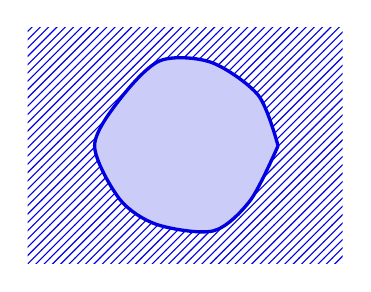
\begin{tikzpicture}
			\fill[cstfille1] (-2,-1.5) rectangle (2,1.5);
			\filldraw[cstcurve,main,cstfill1,smooth] plot coordinates {(1.18,0) (.93,.64) (.33,1.06) (-.32,1.08) (-.83,.59) (-1.15,0) (-.83,-.68) (-.36,-1) (.36,-1.08) (.83,-.69) (1.18,0)};
		\end{tikzpicture}
	\end{center}
\end{frame}


\begin{frame}{单连通区域和多连通区域}
	\onslide<+->
	在前面所说的几个常见区域的例子中, 我们在区域中画一条闭路.
	\onslide<+->
	除了圆环域之外, 闭路的内部仍然包含在这个区域内.
	\onslide<+->
	\begin{definition}
		若区域 $D$ 中的任一闭路的内部都包含在 $D$ 中, 则称 $D$ 是\emph{单连通区域}.
		否则称之为\emph{多连通区域}.
	\end{definition}
	\onslide<+->
	单连通区域内的任一闭路可以``连续地变形''成一个点.
	\onslide<+->
	这也等价于: 设 $\ell_0,\ell_1$ 是从 $A$ 到 $B$ 的两条连续曲线, 则 $\ell_0$ 可以连续地变形为 $\ell_1$ 且保持端点不动.
	\onslide<4->
	\bigdel
	\begin{center}
		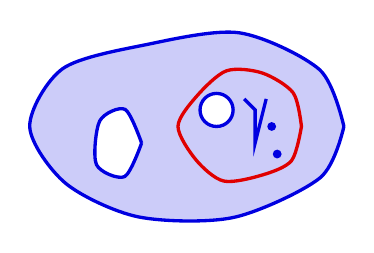
\begin{tikzpicture}[scale=.7]
			\filldraw[cstcurve,main,cstfill1,smooth] plot coordinates {(2.81,0) (2.37,1.03) (.91,1.7) (-.8,1.48) (-2.29,1.05) (-2.89,0) (-2.24,-1.03) (-.92,-1.64) (.81,-1.65) (2.38,-.93) (2.81,0)};
			\filldraw[cstcurve,main,fill=white,smooth] plot coordinates {(-.86,-.3) (-1.16,.31) (-1.62,.1) (-1.68,-.69) (-1.17,-.91) (-.86,-.3)};
			\filldraw[cstcurve,main,fill=white] (.5,.3) circle (.3);
			\fill[cstdot,main] (1.5,0) circle;
			\fill[cstdot,main] (1.6,-.5) circle;
			\draw[cstcurve,main] plot coordinates {(1,.5) (1.2,.3) (1.2,-.3) (1.4,.5)};
			\draw[cstcurve,second,smooth,visible on=<5->,shift={(.1,.2)}] plot coordinates {(1.94,-.2) (1.79,.41) (1.23,.77) (.58,.81) (.04,.35) (-.3,-.2) (.03,-.81) (.53,-1.19) (1.23,-1.08) (1.76,-.82) (1.94,-.2)};
		\end{tikzpicture}
	\end{center}
\end{frame}


\begin{frame}{典型例题: 区域的特性}
	\onslide<+->
	\begin{example}[sidepic,righthand width=3.3cm]
		$\Re(z^2)<1$.
		\onslide<+->{%
			设 $z=x+y\ii$, 则 $\Re(z^2)=x^2-y^2<1$.
		}\onslide<+->{%
			这是无界的单连通区域.
		}
		\tcblower
		\onslide<2->{%
		\begin{center}
			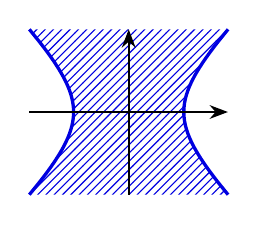
\begin{tikzpicture}[scale=.7]
				\def\t{{atan(1.5)}}
				\fill[cstfille1,domain=-\t:\t,smooth] plot ({sec(\x)},{tan(\x)})
				-- plot[domain=\t:-\t] ({-sec(\x)},{tan(\x)})
				--cycle;
				\draw[cstcurve,main,domain=-\t:\t,smooth] plot ({sec(\x)},{tan(\x)});
				\draw[cstcurve,main,domain=-\t:\t,smooth] plot ({-sec(\x)},{tan(\x)});
				\draw[cstaxis] (-1.8,0)--(1.8,0);
				\draw[cstaxis] (0,-1.5)--(0,1.5);
			\end{tikzpicture}
		\end{center}}
	\end{example}
	\onslide<+->
	\begin{example}[sidepic,righthand width=3.3cm]
		$\arg z\neq \pi$. 
		\onslide<+->{%
			即角状区域 $-\pi<\arg z<\pi$.
		}\onslide<+->{%
			这是无界的单连通区域.
		}
		\tcblower
		\onslide<5->{%
		\begin{center}
			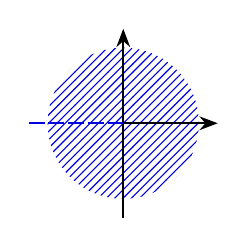
\begin{tikzpicture}[scale=.8]
				\fill[cstfille1] (0,0) circle (1.2);
				\draw[cstaxis] (0,0)--(1.5,0);
				\draw[cstaxis] (0,-1.5)--(0,1.5);
				\draw[cstdash,main] (-1.5,0)--(0,0);
			\end{tikzpicture}
		\end{center}}
	\end{example}
\end{frame}


\begin{frame}{典型例题: 区域的特性}
	\onslide<+->
	\begin{example}[near,sidepic,righthand width=3.3cm]
		$\Bigabs{\dfrac1z}\le3$.
		\onslide<+->{%
			即 $\abs{z}\ge\dfrac13$.
		}\onslide<+->{%
			这是无界的多连通\alertn{闭区域}.
		}
		\tcblower
		\onslide<2->{%
		\begin{center}
			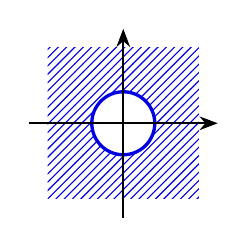
\begin{tikzpicture}[scale=.8]
				\fill[cstfille1] (-1.2,-1.2) rectangle (1.2,1.2);
				\filldraw[cstcurve,main,fill=white] (0,0) circle (.5);
				\draw[cstaxis] (-1.5,0)--(1.5,0);
				\draw[cstaxis] (0,-1.5)--(0,1.5);
			\end{tikzpicture}
		\end{center}}
	\end{example}
	\onslide<+->
	\begin{example}[near,sidepic,righthand width=3.3cm]
		$\abs{z+1}+\abs{z-1}<4$.
		\onslide<+->{%
			表示一个椭圆的内部.
		}\onslide<+->{%
			这是有界的单连通区域.
		}
		
		\tcblower
		\onslide<5->{%
		\begin{center}
			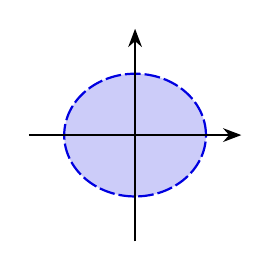
\begin{tikzpicture}[scale=.9]
				\filldraw[cstdash,main,cstfill1] (0,0) circle (1 and {0.5*sqrt(3)});
				\draw[cstaxis] (-1.5,0)--(1.5,0);
				\draw[cstaxis] (0,-1.5)--(0,1.5);
			\end{tikzpicture}
		\end{center}}
	\end{example}
	\onslide<+->
	\begin{exercise}[near]
		$\abs{z+1}+\abs{z-1}\ge 1$ 表示什么集合?
		\onslide<+->{\alertn{整个复平面.}}
	\end{exercise}
\end{frame}


\section{分块矩阵}

\subsection{分块矩阵的定义和运算}

\begin{frame}{分块矩阵的定义}
	\onslide<+->
	有时为了研究矩阵和其部分元素形成的矩阵的联系, 需要使用\emph{分块法}将其进行拆分:
	\onslide<+->
	\begin{definition}[分块矩阵]
		用若干条横线和竖线将矩阵 $\bfA$ 分成许多小矩阵, 每个小矩阵成为 $\bfA$ 的子块, 以子块为元素的矩阵称为\emph{分块矩阵}.
	\end{definition}
	\onslide<+->
	例如
	\[\bfA=\begin{pmatrix}
		\bfO_{m\times n}&\bfE_m\\
		\bfE_n&\bfO_{n\times m}
	\end{pmatrix}\]
	就是一个分块矩阵.
	\onslide<+->
	事实上我们已经不加声明地用过分块矩阵了.
\end{frame}


\begin{frame}{分块矩阵的运算: 加法和数乘}
	\onslide<+->
	若分块矩阵 $\bfA,\bfB$ 同型, 且每个对应分块也同型, 则 $\bfA+\bfB$ 就是对应分块相加形成的分块矩阵:
	\[\begin{pmatrix}
		\bfA_{11}&\cdots&\bfA_{1r}\\
		\vdots&\ddots&\vdots\\
		\bfA_{s1}&\cdots&\bfA_{sr}
	\end{pmatrix}+\begin{pmatrix}
		\bfB_{11}&\cdots&\bfB_{1r}\\
		\vdots&\ddots&\vdots\\
		\bfB_{s1}&\cdots&\bfB_{sr}
	\end{pmatrix}=\begin{pmatrix}
		\bfA_{11}+\bfB_{11}&\cdots&\bfA_{1r}+\bfB_{1r}\\
		\vdots&\ddots&\vdots\\
		\bfA_{s1}+\bfB_{s1}&\cdots&\bfA_{sr}+\bfB_{sr}
	\end{pmatrix}.\]

	\onslide<+->
	数 $\lambda$ 和分块矩阵的数乘, 就是 $\lambda$ 和对应分块数乘形成的分块矩阵:
	\[\lambda\begin{pmatrix}
		\bfA_{11}&\cdots&\bfA_{1r}\\
		\vdots&\ddots&\vdots\\
		\bfA_{s1}&\cdots&\bfA_{sr}
	\end{pmatrix}=\begin{pmatrix}
		\lambda\bfA_{11}&\cdots&\lambda\bfA_{1r}\\
		\vdots&\ddots&\vdots\\
		\lambda\bfA_{s1}&\cdots&\lambda\bfA_{sr}
	\end{pmatrix}.\]
\end{frame}


\begin{frame}{分块矩阵的运算: 乘法}
	\onslide<+->
	设
	\[\bfA=\begin{pmatrix}
		\bfA_{11}&\cdots&\bfA_{1r}\\
		\vdots&\ddots&\vdots\\
		\bfA_{s1}&\cdots&\bfA_{sr}
	\end{pmatrix},\quad
	\bfB=\begin{pmatrix}
		\bfB_{11}&\cdots&\bfB_{1t}\\
		\vdots&\ddots&\vdots\\
		\bfB_{r1}&\cdots&\bfB_{rt},
	\end{pmatrix}\]
	且 $\bfA_{ij}$ 的列数和 $\bfB_{jk}$ 的行数相同, 则
	\[\bfA\bfB=\begin{pmatrix}
		\bfC_{11}&\cdots&\bfC_{1r}\\
		\vdots&\ddots&\vdots\\
		\bfC_{s1}&\cdots&\bfC_{sr}
	\end{pmatrix},\quad\bfC_{ij}=\sum_{k=1}^r \bfA_{ik}\bfB_{kj}.\]
	\onslide<+->
	简单来说就是, 若对应的分块能做相应运算, 则分块矩阵的运算就如同把这些分块视作数一样运算.
\end{frame}


\begin{frame}{分块矩阵的运算: 转置}
	\onslide<+->
	设
	\[\bfA=\begin{pmatrix}
		\bfA_{11}&\cdots&\bfA_{1r}\\
		\vdots&\ddots&\vdots\\
		\bfA_{s1}&\cdots&\bfA_{sr}
	\end{pmatrix},\]
	则
	\[\bfA^\rmT=\begin{pmatrix}
		\bfA_{11}^\rmT&\cdots&\bfA_{s1}^\rmT\\
		\vdots&\ddots&\vdots\\
		\bfA_{1r}^\rmT&\cdots&\bfA_{sr}^\rmT
	\end{pmatrix}.\]
	\onslide<+->
	注意小块的位置需要转置, 每个小块也需要转置.
\end{frame}


\subsection{特殊分块矩阵}
\begin{frame}{分块对角阵}
	\onslide<+->
	若方阵
	\[\bfA=\begin{pmatrix}
		\bfA_1&&\\
		&\ddots&\\
		&&\bfA_m
	\end{pmatrix},\]
	其中 $\bfA_1,\dots,\bfA_m$ 都是方阵,
	\onslide<+->
	称 $\bfA$ 为\emph{分块对角阵}.
	\onslide<+->
	记作 $\bfA=\diag(\bfA_1,\dots,\bfA_m)$.

	\onslide<+->
	分块对角阵具有如下性质:
	\begin{enumerate}
		\item $|\bfA|=|\bfA_1|\cdots|\bfA_m|$;
		\item $\bfA$ 可逆当且仅当 $\bfA_1,\dots,\bfA_m$ 均可逆, 此时
		$\bfA^{-1}=\diag(\bfA_1^{-1},\dots,\bfA_m^{-1})$.
		\item $\bfA^k=\diag(\bfA_1^k,\dots,\bfA_m^k)$.
	\end{enumerate}
\end{frame}


\begin{frame}{例: 分块对角阵}
	\onslide<+->
	\begin{example}
		求 $\bfA=\begin{pmatrix}
			2&1&0&0\\
			1&1&0&0\\
			0&0&2&0\\
			0&0&-1&3
		\end{pmatrix}$ 的逆矩阵.
	\end{example}
	\onslide<+->
	\begin{solution}
		设 $\bfA_1=\begin{pmatrix}
			2&1\\1&1
		\end{pmatrix},\bfA_2=\begin{pmatrix}
			2&0\\-1&3
		\end{pmatrix}$,
		\onslide<+->{%
			则 $\bfA_1^{-1}=\begin{pmatrix}
				1&-1\\-1&2
			\end{pmatrix},\quad\bfA_2^{-1}=\dfrac16\begin{pmatrix}
				3&0\\1&2
			\end{pmatrix}$.
		}

		\onslide<+->{%
			故 $\bfA^{-1}=\diag(\bfA_1^{-1},\bfA_2^{-1})=\begin{pNiceMatrix}
				1&-1&&\\
				-1&2&&\\
				&&1/2&0\\
				&&1/6&1/3
			\end{pNiceMatrix}$.
		}
	\end{solution}
\end{frame}


\begin{frame}{例: 分块三角阵的逆}
\beqskip{2pt}
	\onslide<+->
	\begin{example}
		设 $\bfA,\bfB$ 均可逆, 求 $\begin{pmatrix}
			\bfA&\bfO\\\bfC&\bfB
		\end{pmatrix}$ 的逆矩阵.
	\end{example}
	\onslide<+->
	\begin{solution}
		由 $\begin{vmatrix}
			\bfA&\bfO\\\bfC&\bfB
		\end{vmatrix}=|\bfA|\cdot|\bfB|\neq0$ 可知该方阵可逆.
		\onslide<+->{%
			设 $\begin{pmatrix}
				\bfA&\bfO\\\bfC&\bfB
			\end{pmatrix}\begin{pmatrix}
				\bfA_1&\bfA_2\\\bfA_3&\bfA_4
			\end{pmatrix}=\bfE$.
		}
		
		\onslide<+->{%
			则 $\bfA\bfA_1=\bfE, \bfA\bfA_2=\bfO, \bfC\bfA_2+\bfB\bfA_4=\bfE$.
		}\onslide<+->{%
			于是 $\bfA_1=\bfA^{-1},\bfA_2=\bfO,\bfA_4=\bfB^{-1}$.
		}\onslide<+->{%
			再由 $\bfC\bfA_1+\bfB\bfA_3=\bfO$ 可得
			\[\bfA_3=-\bfB^{-1}\bfC\bfA_1=-\bfB^{-1}\bfC\bfA^{-1}.\]
		}\onslide<+->{%
			故 $\begin{pmatrix}
				\bfA&\bfO\\\bfC&\bfB
			\end{pmatrix}^{-1}=\begin{pmatrix}
				\bfA^{-1}&\bfO\\-\bfB^{-1}\bfC\bfA^{-1}&\bfB^{-1}
			\end{pmatrix}$.
		}
	\end{solution}
	\onslide<+->
	由此可知, (分块)上/下三角阵的逆还是(分块)上/下三角阵.
\endgroup
\end{frame}


\begin{frame}{例: 分块方阵的伴随}
	\onslide<+->
	\begin{exercise}
		设 $\bfA,\bfB$ 为同阶方阵, $\bfC=\begin{pmatrix}
			&\bfA\\\bfB&
		\end{pmatrix}$,
		则 $\bfC^*=$\fillbrace{\visible<+->{D}}.
		\begin{taskschoice}(2)
			() $\begin{pmatrix}&\bfA^*\\\bfB^*&\end{pmatrix}$
			() $\begin{pmatrix}&\bfB^*\\\bfA^*&\end{pmatrix}$
			() $\begin{pmatrix}&|\bfB|\bfA^*\\|\bfA|\bfB^*&\end{pmatrix}$
			() $\begin{pmatrix}&|\bfA|\bfB^*\\|\bfB|\bfA^*&\end{pmatrix}$
		\end{taskschoice}
	\end{exercise}
\end{frame}


\section{极限和连续性}


\subsection{数列的极限}


\begin{frame}{数列的极限}
	\begin{itemize}
		\item 类似于实变函数情形, 我们可以定义复变函数的极限.
		\item 我们先来看数列极限的定义.
	\end{itemize}
	\onslide<+->
	\begin{definition}
		设 $\{z_n\}_{n\ge 1}$ 是一个复数列.
		\onslide<+->{%
		若存在复数 $z$ 满足对任意 $\varepsilon>0$, 存在 $N$ 使得当 $n\ge N$ 时, $\abs{z_n-z}<\varepsilon$, 则称 $z$ 是\emph{数列 $\{z_n\}$ 的极限}, 记作 \emph{$\liml_{n\ra\infty}z_n=z$}.
		}
	\end{definition}
	\begin{itemize}
		\item 此时称\emph{极限存在}或\emph{数列收敛}.
		\item 若不存在这样的 $z$, 则称\emph{极限不存在}或\emph{数列发散}.
		\item 可以看出, $\liml_{n\ra\infty}z_n=z$ 等价于实极限 $\liml_{n\ra\infty}\abs{z_n-z}=0$.
	\end{itemize}
\end{frame}


\begin{frame}{极限的四则运算}
	\begin{itemize}
		\item 由于复数列极限的定义和实数列极限的定义在形式上完全相同,
		\item 因此类似地, 极限的四则运算法则对于复数列也是成立的.
	\end{itemize}
	\onslide<+->
	\begin{theorem}
		设 $\liml_{n\to\infty}z_n=z,\liml_{n\to\infty}w_n=w$, 则
		\begin{enumerate}
			\item $\liml_{n\to\infty}(z_n\pm w_n)=z\pm w$;
			\item $\liml_{n\to\infty} z_nw_n=zw$;
			\item 当 $w\neq 0$ 时, $\liml_{n\to\infty}\dfrac{z_n}{w_n}=\dfrac zw$.
		\end{enumerate}
	\end{theorem}
\end{frame}


\begin{frame}{数列收敛的等价刻画}
	\begin{itemize}
		\item 下述定理保证了我们可以使用实数列的敛散性判定方法来研究复数列的敛散性.
	\end{itemize}
	\onslide<+->
	\begin{theorem}[nearnext]
		设 $z_n=x_n+y_n\ii,z=x+y\ii$, 则
		\[
			\liml_{n\ra\infty}z_n=z\iff
			\liml_{n\ra\infty}x_n=x\ \text{且}\ 
			\liml_{n\ra\infty}y_n=y.
		\]
	\end{theorem}
	\onslide<+->
	\begin{proof}[leftupper=0mm,nearprev]
		\begin{itemize}
			\item 我们只需证明 $
			\liml_{n\ra\infty}\abs{z_n-z}=0\iff
			\liml_{n\ra\infty}\abs{x_n-x}=\liml_{n\ra\infty}\abs{y_n-y}=0$.
			\item ``$\Rightarrow$'': 由三角不等式 $0\le \abs{x_n-x}, \abs{y_n-y}\le\abs{z_n-z}$ 和夹逼准则可得知.
			\item ``$\Leftarrow$'': 由极限的四则运算法则可知 $\liml_{n\ra\infty}\bigl(\abs{x_n-x}+\abs{y_n-y}\bigr)=0$.
			\item 再由三角不等式 $0\le\abs{z_n-z}\le\abs{x_n-x}+\abs{y_n-y}$ 和夹逼准则可得.\qedhere
		\end{itemize}
	\end{proof}
\end{frame}


\begin{frame}{例: 数列的敛散性}
	\onslide<+->
	\begin{example}[nearnext]
		设 $z_n=\Bigl(1-\dfrac1n\Bigr)\ee^{\frac{\pi\ii}n}$. 数列 $\{z_n\}$ 是否收敛?
	\end{example}
	\onslide<+->
	\begin{solution}[nearprev,leftupper=0mm]
		\begin{itemize}
			\item 由于
			\[
				x_n=\Bigl(1-\frac1n\Bigr)\cos\frac\pi n\to 1,\quad
				y_n=\Bigl(1-\frac1n\Bigr)\sin\frac\pi n\to 0.
			\]
			\item 因此 $\{z_n\}$ 收敛且 $\liml_{n\to\infty}z_n=1$.
		\end{itemize}
	\end{solution}
\end{frame}


\subsection{无穷远点和复球面}


\begin{frame}{数列极限的等价定义\noexer}
	\begin{itemize}
		\item 数列极限的定义可以用邻域的语言重新表述为:
	\end{itemize}
	\onslide<+->
	\begin{definition}
		$\liml_{n\ra\infty}z_n=z$ 是指: 对 $z$ 的任意 $\delta$ 邻域 $U$, 存在 $N$ 使得当 $n\ge N$ 时, $z_n\in U$.
	\end{definition}
	\begin{itemize}
		\item 若 $\liml_{n\ra\infty}\abs{z_n}=+\infty$, 我们将其记为 \emph{$\liml_{n\ra\infty}z_n=\infty$}.
		\item 这也等价于: 对任意 $X>0$, 存在 $N$ 使得当 $n\ge N$ 时, $\abs{z_n}>X$.
		\item 我们能不能也用邻域的语言来描述 $\liml_{n\ra\infty}z_n=\infty$ 呢?
		\item 我们将介绍复球面的概念, 它是复数的一种几何表示方式且自然地包含无穷远点 $\infty$.
		\item 这种思想是在黎曼研究多值复变函数时引入的.
	\end{itemize}
\end{frame}


\begin{frame}[b]{复球面\noexer}
	\begin{itemize}
		\item 取一个球心在 $z=0$ 的单位球面.
		\item 过 $O$ 做垂直于复平面的直线, 并与球面相交于其中一点 $N$, 称之为北极.
		\item 对于平面上的任意一点 $z$, 连接北极 $N$ 和 $z$ 的直线一定与球面相交于除 $N$ 以外的唯一一个点 $Z$.
		\item 反之, 球面上除了北极外的任意一点 $Z$, 直线 $NZ$ 一定与复平面相交于唯一一点.
		\item 这样, 球面上除北极外的所有点和全体复数建立了一一对应.
	\end{itemize}
	\onslide<1->
	\begin{center}
		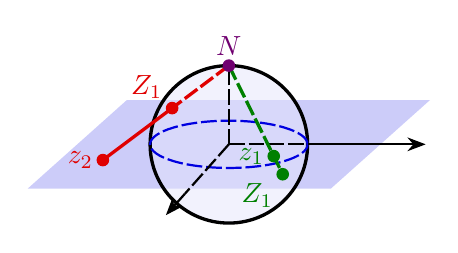
\begin{tikzpicture}
			\begin{scope}[scale=1]
				\fill[cstfill1,scale=.7] (-3.65,-.804)--(-1.85,.804)--(3.65,.804)--(1.85,-.804)--cycle;
				\filldraw[cstcurve,fill=main!10,fill opacity=.5] (0,0) circle (1);
				\draw[cstdash,main] (0,0) circle (1 and 0.3);
				\coordinate [visible on=<2->] (N) at (0,1);
				\draw[cstdash,visible on=<2->] (0,0)--(N);
				\draw[cstdash] (0,0)--(1,0);
				\draw[cstaxis] (1,0)--(2.5,0);
				\def\a{.7}
				\draw[cstdash] (0,0)--({-.8*\a},{-.9*\a});
				\draw[cstaxis] ({-.8*\a},{-.9*\a})--(-.8,-.9);
				\coordinate [visible on=<3->] (z1) at (.57,-.15);
				\coordinate [visible on=<3->] (Z1) at ($(N)!1.2!(z1)$);
				\coordinate [visible on=<4->] (z2) at (-1.6,-.2);
				\coordinate [visible on=<4->] (Z2) at ($(N)!.45!(z2)$);
				\draw[cstdash,cstcurve,fourth,visible on=<3->] (N)--(Z1);
				\draw[cstdash,cstcurve,second,visible on=<4->] (N)--(Z2);
				\draw[cstcurve,second,visible on=<4->] (Z2)--(z2);
			\end{scope}
			\fill[cstdot,fourth,visible on=<3->] (Z1) circle;
			\fill[cstdot,second,visible on=<4->] (Z2) circle;
			\fill[cstdot,fourth,visible on=<3->] (z1) circle;
			\fill[cstdot,second,visible on=<4->] (z2) circle;
			\fill[cstdot,third,visible on=<2->] (N) circle;
			\draw (N) node[third,above,visible on=<2->] {$N$};
			\draw (z1) node[fourth,left,visible on=<3->] {$z_1$};
			\draw (Z1) node[fourth,below left,visible on=<3->] {$Z_1$};
			\draw (z2) node[second,left,visible on=<4->] {$z_2$};
			\draw (Z2) node[second,above left,visible on=<4->] {$Z_1$};
		\end{tikzpicture}
	\end{center}
\end{frame}


\begin{frame}[b]{复球面: 无穷远点\noexer}
	\begin{itemize}
		\item 当 $|z|$ 越来越大时, 其对应球面上点也越来越接近 $N$.
		\item 如果我们在复平面上添加一个额外的"点"——\emph{无穷远点}, 记作 \emph{$\infty$}.
		\item 那么\emph{扩充复数集合 $\BC^*=\BC\cup\{\infty\}$} 就正好和球面上的点一一对应.
		\item 称这样的球面为\emph{复球面}, 称包含无穷远点的复平面为\emph{扩充复平面}或\emph{闭复平面}.
	\end{itemize}
	\onslide<1->
	\begin{center}
		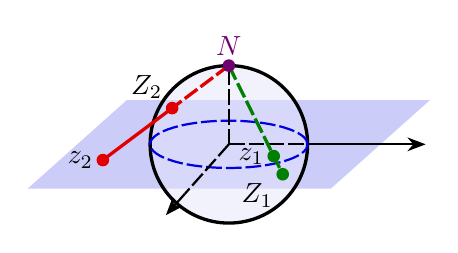
\begin{tikzpicture}
			\begin{scope}[scale=1]
				\fill[cstfill1,scale=.7] (-3.65,-.804)--(-1.85,.804)--(3.65,.804)--(1.85,-.804)--cycle;
				\filldraw[cstcurve,fill=main!10,fill opacity=.5] (0,0) circle (1);
				\draw[cstdash,main] (0,0) circle (1 and 0.3);
				\coordinate [label=above:\textcolor{third}{$N$}] (N) at (0,1);
				\draw[cstdash] (0,0)--(N);
				\draw[cstdash] (0,0)--(1,0);
				\draw[cstaxis] (1,0)--(2.5,0);
				\def\a{.7}
				\draw[cstdash] (0,0)--({-.8*\a},{-.9*\a});
				\draw[cstaxis] ({-.8*\a},{-.9*\a})--(-.8,-.9);
				\coordinate [label=left:{$z_1$}] (z1) at (.57,-.15);
				\coordinate [label=below left:{$Z_1$}] (Z1) at ($(N)!1.2!(z1)$);
				\coordinate [label=left:{$z_2$}] (z2) at (-1.6,-.2);
				\coordinate [label=above left:{$Z_2$}] (Z2) at ($(N)!.45!(z2)$);
				\draw[cstdash,cstcurve,fourth] (N)--(Z1);
				\draw[cstdash,cstcurve,second] (N)--(Z2);
				\draw[cstcurve,second] (Z2)--(z2);
			\end{scope}
			\fill[cstdot,fourth] (Z1) circle;
			\fill[cstdot,second] (Z2) circle;
			\fill[cstdot,fourth] (z1) circle;
			\fill[cstdot,second] (z2) circle;
			\fill[cstdot,third] (N) circle;
		\end{tikzpicture}
	\end{center}
\end{frame}


\begin{frame}{复球面: 无穷远点的邻域\noexer}
	\begin{itemize}
		\item 若约定 $\abs{\infty}=+\infty$, 则分别称
		\[
			U(\infty,X)=\{z\in\BC^*\midcolon \abs{z}>X\},\quad
			\Uc(\infty,X)=\{z\in\BC\midcolon \abs{z}>X\}
		\]
		为 $\infty$ 的 \emph{$X$ 邻域}和\emph{去心 $X$ 邻域}.
		\item 这样, 前述极限可统一表述为: 若对 $z\in\BC^*$ 的任意 $\delta$ 邻域 $U$, 存在 $N$ 使得当 $n\ge N$ 时, $z_n\in U$, 则记 $\liml_{n\ra\infty}z_n=z$.
		\item 朴素地看, 复球面上任意一点可以定义 $\delta$ 邻域为与其距离小于 $\delta$ 的所有点.
		\item 特别地, $\infty$ 的邻域通过前面所说的对应关系, 可以对应到扩充复平面上 $\infty$ 的一个邻域.
		\item 所以在复球面上, 普通复数和 $\infty$ 的邻域具有同等地位.
	\end{itemize}
\end{frame}


\begin{frame}{复球面: 与实数无穷的联系\noexer}
	\begin{itemize}
		\item 它和实数列极限符号中的 $\infty$ 有什么联系呢?
		\item 选取上述图形的一个截面来看, 实轴可以和圆周去掉一点建立一一对应.
		\item 于是实数列极限符号中的 $\infty$ 在复球面上就是 $\infty$.
	\end{itemize}
	\onslide<2->
	\begin{center}
		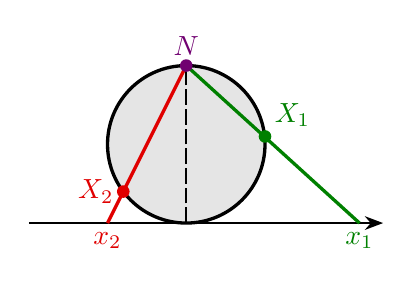
\begin{tikzpicture}
			\filldraw[cstcurve,cstfill] (0,1) circle (1);
			\coordinate [label=above:\textcolor{third}{$N$}] (N) at (0,2);
			\draw[cstdash] (0,0)--(N);
			\draw[cstaxis] (-2,0)--(2.5,0);
			\coordinate [label=below:\textcolor{fourth}{$x_1$}] (x1) at (2.2,0);
			\coordinate [label=above right:\textcolor{fourth}{$X_1$}] (X1) at (1,1.1);
			\coordinate [label=below:\textcolor{second}{$x_2$}] (x2) at (-1,0);
			\coordinate [label=left:\textcolor{second}{$X_2$}] (X2) at (-.8,.4);
			\draw[cstcurve,fourth] (0,2)--(x1);
			\fill[cstdot,fourth] (X1) circle;
			\draw[cstcurve,second] (0,2)--(x2);
			\fill[cstdot,second] (X2) circle;
			\fill[cstdot,third] (N) circle;
		\end{tikzpicture}
	\end{center}
\end{frame}


\subsection{函数的极限}


\begin{frame}{函数的极限}
	\onslide<+->
	\begin{definition}
		设函数 $f(z)$ 在点 $z_0$ 的某个去心邻域内有定义.
		\onslide<+->{%
			如果存在复数 $A$, 使得对 $A$ 的任意邻域 $U(A,\varepsilon),\exists\delta>0$ 使得
			\[z\in\Uc(z_0,\delta)\implies f(z)\in U(A,\varepsilon),
	\]
		}\onslide<+->{%
			则称 $A$ 为 \emph{$f(z)$ 当 $z\to z_0$ 时的极限}, 记为 \emph{$\liml_{z\to z_0}f(z)=A$} 或 \emph{$f(z)\to A (z\to z_0)$}.
		}
	\end{definition}
	\begin{itemize}
		\item 在此表述下, 将上述定义中的 $z_0$ 或 $A$ 换成 $\infty$, 即可得到 $z\ra\infty$ 时的极限定义, 以及 $\lim f(z)=\infty$ 的含义.
	\end{itemize}
\end{frame}


\begin{frame}{极限的四则运算}
	\begin{itemize}
		\item 类似于复数列情形, 极限的四则运算法则对于复变函数也是成立的.
	\end{itemize}
	\onslide<+->
	\begin{theorem}
		设 $\liml_{z\to z_0}f(z)=A,\liml_{z\to z_0}g(z)=B$, 则
		\begin{enumerate}
			\item $\liml_{z\to z_0}(f\pm g)(z)=A\pm B$;
			\item $\liml_{z\to z_0}(fg)(z)=AB$;
			\item 当 $B\neq 0$ 时, $\liml_{z\to z_0}\Bigl(\dfrac fg\Bigr)(z)=\dfrac AB$.
		\end{enumerate}
	\end{theorem}
\end{frame}


\begin{frame}{与实函数极限之联系}
	\begin{itemize}
		\item 和数列极限类似, 我们有下述定理:
	\end{itemize}
	\onslide<+->
	\begin{theorem}
		设 $f(z)=u(x,y)+\ii v(x,y),z_0=x_0+y_0\ii,A=u_0+v_0\ii$, 则
		\[
			\lim_{z\to z_0}f(z)=A\iff
			\lim_{\substack{x\to x_0\\y\to y_0}}u(x,y)=u_0,\quad
			\lim_{\substack{x\to x_0\\y\to y_0}}v(x,y)=v_0.
		\]
	\end{theorem}
	\begin{itemize}
		\item 该定理表明: 研究复变函数极限, 只需研究其实部、虚部两个二元实函数的极限.
		\item 在学习了复变函数的导数后, 我们也可以使用等价无穷小替换、洛必达法则等工具来计算极限.
	\end{itemize}
\end{frame}


\begin{frame}{例: 判断函数极限是否存在}
	\onslide<+->
	\begin{example}[nearnext]
		证明: 当 $z\to0$ 时, 函数 $f(z)=\dfrac{\Re z}{|z|}$ 的极限不存在.
	\end{example}
	\onslide<+->
	\begin{proof}[leftupper=0mm,nearprev]
		\begin{itemize}
			\item 令 $z=x+y\ii$, 则 $f(z)=\dfrac x{\sqrt{x^2+y^2}}$.
			\item 因此
			\[
				u(x,y)=\frac x{\sqrt{x^2+y^2}},\quad v(x,y)=0.
			\]
			\item 当 $z$ 在实轴原点两侧分别趋向于 $0$ 时, $u(x,y)\to\pm1$.
			\item 因此 $\liml_{\substack{x\to 0\\y\to0}}u(x,y)$ 不存在, 从而 $\liml_{z\to z_0}f(z)$ 不存在.\qedhere
		\end{itemize}
		\meddel
	\end{proof}
\end{frame}


\subsection{函数的连续性}


\begin{frame}{函数的连续性}
	\onslide<+->
	\begin{definition}[nearprev]
		\begin{enumerate}
			\item 如果 $\liml_{z\to z_0}f(z)=f(z_0)$, 则称 $f(z)$ 在 \emph{$z_0$ 处连续}.
			\item 如果 $f(z)$ 在区域 $D$ 内处处连续, 则称 $f(z)$ 在 \emph{$D$ 内连续}.
		\end{enumerate}
	\end{definition}
	\onslide<+->
	根据前面的极限判定定理可知:
	\onslide<+->
	\begin{theorem}[nearnext]
		\begin{enumerate}
			\item 函数 $f(z)=u(x,y)+\ii v(x,y)$ 在 $z_0=x_0+\ii y_0$ 处连续当且仅当 $u(x,y)$ 和 $v(x,y)$ 在 $(x_0,y_0)$ 处连续.
			\item 在 $z_0$ 处连续的两个函数 $f(z)$, $g(z)$ 之和、差、积、商($g(z_0)\neq 0$) 在 $z_0$ 处仍然连续.
			\item 如果函数 $g(z)$ 在 $z_0$ 处连续, 函数 $f(w)$ 在 $g(z_0)$ 处连续, 则 $f(g(z))$ 在 $z_0$ 处连续.
		\end{enumerate}
	\end{theorem}
\end{frame}


\begin{frame}{连续函数的性质}
	\onslide<+->
	\begin{example}[near]
		\begin{enumerate}
			\item 设 $f(z)=\ln(x^2+y^2)+\ii(x^2-y^2)$.
			\onslide<+->{%
			$u(x,y)=\ln(x^2+y^2)$ 除原点外处处连续, $v(x,y)=x^2-y^2$ 处处连续.
			}\onslide<+->{%
			因此 $f(z)$ 在 $z\neq0$ 处连续.
			}
			\item 显然 $f(z)=z$ 是处处连续的,
			\onslide<+->{%
			故多项式函数
			\[
				P(z)=a_0+a_1z+a_2z^2+\cdots+a_nz^n
			\]
			也处处连续,
			}\onslide<+->{%
			有理函数 $\dfrac{P(z)}{Q(z)}$ 在 $Q(z)$ 的零点以外处处连续.
			}
		\end{enumerate}
	\end{example}
\end{frame}


\begin{frame}{例: 函数连续性的判定}
	\onslide<+->
	\begin{example}[near]
		证明: 如果 $f(z)$ 在 $z_0$ 连续, 则 $\ov{f(z)}$ 在 $z_0$ 也连续.
	\end{example}
	\onslide<+->
	\begin{proof}[near,leftupper=0mm]
		\begin{itemize}
			\item 设 $f(z)=u(x,y)+\ii v(x,y),z_0=x_0+\ii y_0$.
			\item 那么 $u(x,y),v(x,y)$ 在 $(x_0,y_0)$ 连续.
			\item 从而 $-v(x,y)$ 也在 $(x_0,y_0)$ 连续.
			\item 所以 $\ov{f(z)}=u(x,y)-\ii v(x,y)$ 在 $(x_0,y_0)$ 连续.\qedhere
		\end{itemize}
	\end{proof}
	\onslide<+->
	\begin{proof}[near,leftupper=0mm][另证]
		\begin{itemize}
			\item 函数 $g(z)=\ov z=x-\ii y$ 处处连续,
			\item 从而 $g(f(z))=\ov{f(z)}$ 在 $z_0$ 处连续.\qedhere
		\end{itemize}
	\end{proof}
\end{frame}


\begin{frame}{注记}
	\begin{itemize}
		\item 可以看出, 在极限和连续性上, 复变函数和两个二元实函数没有什么差别.
		\item 那么复变函数和多变量微积分的差异究竟是什么导致的呢?
		\item 归根到底就在于 $\BC$ 是一个域, 上面可以做除法.
		\item 这就导致了复变函数有\alert{导数}, 而不是像多变量实函数只有偏导数.
		\item 这种特性使得可导的复变函数具有整洁优美的性质, 我们将在下一章来逐步揭开它的神秘面纱.
	\end{itemize}
\end{frame}



\part{解析函数}
\section{向量组}

\subsection{向量组的线性表示}

\begin{frame}{引例题: 齐次线性方程组的解}
	\onslide<+->
	我们知道齐次线性方程组是指 $\bfA\bfx={\bf0}$.
	\onslide<+->
	令
	\[V=\{\bfx\mid \bfA\bfx={\bf0}\}\]
	表示该方程的所有解形成的集合.
	\onslide<+->
	显然 ${\bf0}\in V$.
	\onslide<+->
	若 $\bfu,\bfv\in V$, 则 $\bfA\bfu=\bfA\bfv={\bf0}$.
	\onslide<+->
	于是
	\[\bfA(\bfu+\bfv)=\bfA(\lambda \bfv)={\bf0},\quad \forall\lambda\in\BC.\]
	\onslide<+->
	换言之, $V$ 上的加法和数乘的结果还落在 $V$ 中.
	\onslide<+->
	它是 $\BC^n$ 的一个\emph{子空间}.
	
	\onslide<+->
	如何用有限个向量来表示一个子空间中的所有向量呢?
	\onslide<+->
	我们需要线性组合的概念.
\end{frame}


\begin{frame}{向量组}
	\onslide<+->
	一些具有相同维数的向量放在一起形成\emph{向量组}(可以有重复的):
	\onslide<+->
	例如:
	\begin{itemize}
		\item $\bma_1=(1,1,-1)^\rmT, \bma_2=(2,1,2)^\rmT, \bma_3=(3,2,1)^\rmT$;
		\item $\bma_1^\rmT=(1,1,-1), \bma_2^\rmT=(2,1,2), \bma_3^\rmT=(3,2,1)$;
		\item $m\times n$ 矩阵 $\bfA$ 的 $m$ 行可以看成 $m$ 个行向量, 它们构成一个向量组, 叫做 $\bfA$ 的\emph{行向量组};
		\item 类似地, $\bfA$ 的列向量构成它的\emph{列向量组}.
		\item 对于 $n$ 维向量组
		\[\bfe_1=(1,0,\dots,0)^\rmT,\bfe_2=(0,1,\dots,0)^\rmT,\dots,\bfe_n=(0,0,\dots,1)^\rmT,\]
		\onslide<+->{%
			任意 $n$ 维向量 $\bfx=(x_1,\dots,x_n)^\rmT$ 可以表示为这个向量组中向量的数乘之和:
			\[\bfx=x_1\bfe_1+\cdots+x_n\bfe_n.\]
		}
	\end{itemize}
\end{frame}


\begin{frame}{向量组的线性表示}
	\onslide<+->
	\begin{definition}
		设 $\bma_1,\dots,\bma_m,\bmb$ 为 $n$ 维向量.
		若存在数 $\lambda_1,\dots,\lambda_m$ 使得
		\[\bmb=\lambda_1\bma_1+\cdots+\lambda_m\bma_m,\]
		则称 $\bmb$ 可以被向量组 $\{\bma_1,\dots,\bma_m\}$ \emph{线性表示}, 或称 $\bmb$ 是向量组 $\{\bma_1,\dots,\bma_m\}$ 的\emph{线性组合}.
	\end{definition}
	\onslide<+->
	\begin{example}
		\begin{enumerate}
			\item $n$ 维零向量是任一 $n$ 维向量组的线性组合.
			\item 任意 $n$ 维向量是 $\bfe_1,\dots,\bfe_n$ 的线性组合.
		\end{enumerate}
	\end{example}
\end{frame}


\begin{frame}{线性表示的等价刻画}
	\onslide<+->
	向量 $\bmb$ 能被向量组 $\bma_1,\dots,\bma_m$ 线性表示, 即存在 $\lambda_1,\dots,\lambda_m$ 使得
	\[\bmb=\lambda_1\bma_1+\cdots+\lambda_m\bma_m=(\bma_1,\dots,\bma_m)\begin{pmatrix}
		\lambda_1\\\vdots\\\lambda_m
	\end{pmatrix}.\]
	\vspace{-\baselineskip}
	\onslide<+->
	\begin{theorem}
		向量 $\bmb$ 能被向量组 $\bma_1,\dots,\bma_m$ 线性表示, 当且仅当 $\bfA\bfx=\bmb$ 有解, 其中
		\[\bfA=(\bma_1,\dots,\bma_m)\in M_{n\times m}.\]
	\end{theorem}
	\onslide<+->
	记 $V$ 为向量组 $S=\{\bma_1,\dots,\bma_m\}$ 能线性表示的向量全体.
	\onslide<+->
	容易知道
	\[V=\{\bmb\in\BC^n\mid \text{存在 $\bfx$ 使得}\ \bfA\bfx=\bmb\}\]
	是 $\BC^n$ 的子空间, 称为 $S$ \emph{生成的空间}.
	\onslide<+->
	它是包含 $S$ 中所有向量的最小的线性空间.
\end{frame}


\begin{frame}{向量组的等价}
	\begin{definition}
		\begin{enumerate}
			\item 设有两个向量组 $S=\{\bma_1,\dots,\bma_m\}, T=\{\bmb_1,\dots,\bmb_k\}$.
			若 $\bmb_1,\dots,\bmb_k$ 均可以被 $\{\bma_1,\dots,\bma_m\}$ 线性表示, 则称向量组 $T$ 可以被向量组 $S$ 线性表示.
			\item 若向量组 $S$ 和 $T$ 能相互线性表示, 则称 $S,T$ \emph{向量组等价}.
		\end{enumerate}
	\end{definition}
	\onslide<+->
	设 $S,T$ 分别生成空间 $V,W$.
	\onslide<+->
	$T$ 可以被 $S$ 线性表示$\iff$ $W\subseteq V$;
	\onslide<+->
	$S,T$ 向量组等价$\iff W=V$.

	\onslide<+->
	$T$ 能被 $S$ 线性表示, 当且仅当存在 $\bfx_1,\dots,\bfx_k$ 使得
	\[\bfA\bfx_1=\bmb_1,\quad\dots,\quad\bfA\bfx_k=\bmb_k,\]
	其中 $\bfA=(\bma_1,\dots,\bma_m)$.
	\onslide<+->
	即存在矩阵 $\bfX$ 使得 $\bfA\bfX=\bfB$, 其中 $\bfB=(\bmb_1,\dots,\bmb_k)$.

	\onslide<+->
	反过来, 若 $\bfA\bfX=\bfB$, 则 $\bfB$ 的列向量组可以由 $\bfA$ 的列向量组线性表示.
\end{frame}


\begin{frame}{向量组的等价}
	\onslide<+->
	\begin{theorem}
		\begin{enumerate}
			\item $\bfB$ 的列向量组可以由 $\bfA$ 的列向量组线性表示$\iff$存在矩阵 $\bfX$ 使得 $\bfB=\bfA\bfX$.
			\item $\bfA$ 的列向量组和 $\bfB$ 的列向量组作为向量组等价$\iff$存在矩阵 $\bfX,\bfY$ 使得 $\bfB=\bfA\bfX,\bfA=\bfB\bfY$.
		\end{enumerate}
	\end{theorem}
	\onslide<+->
	\begin{proposition}
		向量组的等价满足如下性质:
		\begin{enumerate}
			\item 自反性: $S\sim S$;
			\item 对称性: $S\sim T\implies T\sim S$;
			\item 传递性: $S\sim T,T\sim R\implies S\sim R$.
		\end{enumerate}
	\end{proposition}
\end{frame}


\subsection{线性相关与线性无关}

\begin{frame}{线性相关与线性无关}
	\onslide<+->
	\begin{definition}
		对于 $n$ 维向量组 $\{\bma_1,\dots,\bma_m\}$,
		若存在一组\alert{不全为零}的数 $\lambda_1,\dots,\lambda_m$ 使得
		\[\lambda_1\bma_1+\dots+\lambda_m\bma_m={\bf0},\]
		则称该向量组\emph{线性相关}.
		否则称该向量组\emph{线性无关}.
	\end{definition}
	\onslide<+->
	向量组 $\{\bma_1,\dots,\bma_m\}$ 线性无关当且仅当
	\[\lambda_1\bma_1+\dots+\lambda_m\bma_m={\bf0}\implies
	\lambda_1=\cdots=\lambda_m=0.\]
	\onslide<+->
	即 $(\bma_1,\cdots,\bma_m)\bfx={\bf0}$ 只有零解.
\end{frame}


\begin{frame}{例题: 线性相关与线性无关}
	\begin{example}
		\begin{enumerate}
			\item $\bma_1=(1,2,3)^\rmT,\bma_2=(2,3,4)^\rmT,\bma_3=(0,0,0)^\rmT$ 线性相关.
			实际上\alert{包含零向量的向量组总是线性相关的}.
			\item $\bma_1=(1,2,3)^\rmT,\bma_2=(2,4,6)^\rmT,\bma_3=(3,0,5)^\rmT$ 线性相关.
			\alert{线性相关的向量组添加更多向量还是线性相关的}.
			\item $\bma_1=(1,2,3)^\rmT,\bma_2=(2,3,4)^\rmT,\bma_3=(3,5,7)^\rmT$ 线性相关.
			它们构成的 $3$ 阶矩阵行列式为零.
			\alert{$n$ 维向量组 $\bma_1,\dots,\bma_n$ 线性无关 $\iff |\bma_1,\cdots,\bma_n|\neq 0$}.
			\item $\bfe_1=(1,0,0)^\rmT,\bfe_2=(0,1,0)^\rmT,\bfe_3=(0,0,1)^\rmT$ 线性无关.
			一般地, \alert{$n$ 维单位向量组 $\bfe_1,\dots,\bfe_n$ 线性无关}.
			\item $\bma$ 线性相关 $\iff \bma\neq{\bf0}$.
			\item $\bma_1,\bma_2$ 线性相关 $\iff \bma_1,\bma_2$ 对应分量成比例.
		\end{enumerate}
	\end{example}
\end{frame}


\begin{frame}{例题: 判断线性无关}
	\onslide<+->
	\begin{example}
		已知向量组 $\{\bma_1,\bma_2,\bma_3\}$ 线性无关, 证明向量组 $\{\bma_1+\bma_2,\bma_2+\bma_3,\bma_3+\bma_1\}$ 线性无关.
	\end{example}
	\onslide<+->
	\begin{proof}
		设 $\bfA=\begin{pmatrix}
			1&1&0\\
			0&1&1\\
			1&0&1
		\end{pmatrix}$,
		\onslide<+->{则 $|\bfA|=2$, $\bfA$ 可逆,
		}\onslide<+->{%
			且
			\[(\bma_1+\bma_2,\bma_2+\bma_3,\bma_3+\bma_1)=(\bma_1,\bma_2,\bma_3)\bfA.\]
		}\onslide<+->{%
			若 $(\bma_1+\bma_2,\bma_2+\bma_3,\bma_3+\bma_1)\bfx={\bf0}$, 则
			\[(\bma_1,\bma_2,\bma_3)\bfA\bfx={\bf0}\implies
			\bfA\bfx={\bf0}\implies\bfx={\bf0}.\qedhere\]
		}\vspace{-\baselineskip}
	\end{proof}
\end{frame}


\begin{frame}{例题: 判断线性无关}
	\onslide<+->
	\begin{exercise}
		已知向量组 $\{\bma_1,\bma_2\}$ 线性无关, 请问向量组 $\{\bma_1-\bma_2,\bma_1+\bma_2,\bma_1\}$ 是否线性无关?
	\end{exercise}
	\onslide<+->
	\begin{answer}
		线性相关, 因为 $(\bma_1-\bma_2)+(\bma_1+\bma_2)-2\bma_1={\bf0}$.
	\end{answer}
	\onslide<+->
	\begin{exercise}
		设 $\bfA=\begin{pmatrix}
			1&2&-2\\
			2&1&2\\
			3&0&4
		\end{pmatrix},\bma=\begin{pmatrix}
			k\\1\\1
		\end{pmatrix}$.
		若 $\bfA\bma$ 和 $\bma$ 线性相关, 则 $k=$\fillblank{\visible<+->{$-1$}}.
	\end{exercise}
\end{frame}



\subsection{线性相关和线性无关的性质}

\begin{frame}{线性相关和线性无关的等价刻画}
	\onslide<+->
	\begin{theorem}
		向量组 $\bma_1,\dots,\bma_m$ 线性相关$\iff$其中至少有一个向量可以由其它向量线性表示.
	\end{theorem}
	\onslide<+->
	\begin{proof*}
		若该向量组线性相关, 则存在不全为零的数 $\lambda_1,\dots,\lambda_m$ 使得
		\[\lambda_1\bma_1+\cdots+\lambda_m\bma_m={\bf0}.\]
		\onslide<+->{%
			设 $\lambda_i\neq 0$, 则
			$\bma_i=-\displaystyle\frac1{\lambda_i}\sum_{\substack{j=1\\j\neq i}}^m \lambda_j \bma_j$
			可由其它向量线性表示.
		}

		\onslide<+->{
			反之, 若 $\bma_i=\displaystyle\sum_{\substack{j=1\\j\neq i}}^m \lambda_j \bma_j$ 
			可由其它向量线性表示.
		}\onslide<+->{%
			则 $\displaystyle -\bma_i+\sum_{\substack{j=1\\j\neq i}}^m \lambda_j \bma_j={\bf0}$, 
			向量组 $\bma_1,\dots,\bma_m$ 线性相关.\qedhere
		}
	\end{proof*}
\end{frame}


\begin{frame}{线性相关和线性无关的等价刻画}
	\onslide<+->
	向量组 $\bma_1,\dots,\bma_m$ 线性无关$\iff$其中任一向量不可以由其它向量线性表示.

	\onslide<+->
	注意, 向量组 $\bma_1,\dots,\bma_m$ 线性相关\alert{$\ \ \not\!\!\!\!\implies$}其中任一向量可以由其它向量线性表示.
	\onslide<+->
	\begin{exercise}
		设 $\bma_1,\dots,\bma_m$ 是 $m$ 个 $n$ 维向量, 则下列结论是否正确的有\fillblank{\visible<8->{1}}个.
		\begin{enumerate}
			\item {若 $\bma_1,\dots,\bma_m$ 线性相关, 则其中任一向量均可由其余向量线性表示}%
			\item {若 $\bma_m$ 不能由 $\bma_1,\dots,\bma_{m-1}$ 线性表示, 则向量组 $\bma_1,\dots,\bma_m$ 线性无关}%
			\item {若 $\bma_1,\dots,\bma_m$ 线性相关, 且存在不全为零的 $\lambda_1,\dots,\lambda_{m-1}$ 使得\\ $\lambda_1\bma_1+\cdots+\lambda_{m-1}\bma_{m-1}={\bf0}$, 则 $\bma_m$ 不能由 $\bma_1,\dots,\bma_{m-1}$ 线性表示}%
			\item {若 $\bma_1,\dots,\bma_m$ 线性相关, 且 $\bma_m$ 不能由 $\bma_1,\dots,\bma_m$ 线性表示, 则 $\bma_1,\dots,\bma_{m-1}$ 线性相关}
		\end{enumerate}
	\end{exercise}
\end{frame}


\begin{frame}{线性相关和线性无关的性质}
\beqskip{3mm}
	\onslide<+->
	\begin{theorem}
		若向量组 $\bma_1,\dots,\bma_m$ 线性无关, 向量组 $\bma_1,\dots,\bma_m,\bmb$ 线性相关, 则 $\bmb$ 可以由 $\bma_1,\dots,\bma_m$ 线性表示, 且表达形式唯一.
	\end{theorem}
	\onslide<+->
	\begin{proof*}
		存在不全为零的数 $\lambda_1,\dots,\lambda_m,k$ 使得
		\[\lambda_1\bma_1+\cdots+\lambda_m\bma_m+k\bmb={\bf0}.\]
		\onslide<+->{%
			若 $k=0$, 则 $\lambda_1,\dots,\lambda_m$ 不全为零且
			$\lambda_1\bma_1+\cdots+\lambda_m\bma_m={\bf0}$.
		}\onslide<+->{%
			这与 $\bma_1,\dots,\bma_m$ 线性无关矛盾. 因此 $k\neq 0$.
		}
		\onslide<+->{%
			于是 $\bmb$ 可由 $\bma_1,\dots,\bma_m$ 线性表示.
		}

		\onslide<+->{
			若 $\bmb$ 有两种线性表达形式, 二式相减得到不全为零的数 $\lambda_1,\dots,\lambda_m,k$ 使得
			\[\lambda_1\bma_1+\cdots+\lambda_m\bma_m+k\bmb={\bf0}.\]
			矛盾.\qedhere
		}
	\end{proof*}
\endgroup
\end{frame}


\begin{frame}{线性相关和线性无关的性质}
	\onslide<+->
	\begin{theorem}
		设向量组 $S=\{\bma_1,\dots,\bma_m\},T=\{\bma_1,\dots,\bma_m,\bma_{m+1},\dots,\bma_s\}$.
		\begin{enumerate}
			\item 若向量组 $S$ 线性相关, 则 $T$ 也线性相关.
			\item 若向量组 $T$ 线性无关, 则 $S$ 也线性无关.
		\end{enumerate}
	\end{theorem}
	\onslide<+->
	即\alert{部分相关$\implies$整体相关, 整体无关$\implies$部分无关}.
	\onslide<+->
	\begin{example}
		$n$ 维向量组 $\bma_1,\dots,\bma_s (3\le s\le n)$ 线性无关$\iff$\fillbrace{\visible<+->{D}}
		\xx{$\bma_1,\dots,\bma_s$ 中存在一个向量不能由其余向量线性表示}%
		{$\bma_1,\dots,\bma_s$ 中任两个向量都线性无关}%
		{$\bma_1,\dots,\bma_s$ 中不含零向量}%
		{$\bma_1,\dots,\bma_s$ 中任一个向量都不能由其余向量线性表示}
	\end{example}
\end{frame}


\begin{frame}{例题: 线性相关和线性无关}
	\onslide<+->
	\begin{exercise}
		若向量组 $\bma,\bmb,\bmg$ 线性无关, $\bma,\bmb,\bmd$ 线性相关, 则\fillbrace{\visible<+->{C}}.
		\xx{$\bma$ 一定能由 $\bmb,\bmg,\bmd$ 线性表示}%
		{$\bmb$ 一定不能由 $\bma,\bmg,\bmd$ 线性表示}%
		{$\bmd$ 一定能由 $\bma,\bmb,\bmg$ 线性表示}%
		{$\bmd$ 一定不能由 $\bma,\bmb,\bmg$ 线性表示}
	\end{exercise}
	\onslide<+->
	\begin{example}
		设向量 $\bmb$ 可由 $\bma_1,\dots,\bma_m$ 线性表示, 但不能由向量组 $S=\{\bma_1,\dots,\bma_{m-1}\}$ 线性表示. 记 $T=\{\bma_1,\dots,\bma_{m-1},\bmb\}$, 则\fillbrace{\visible<+->{B}}.
		\xx{$\bma_m$ 不能由 $S$ 线性表示, 也不能由 $T$ 线性表示}%
		{$\bma_m$ 不能由 $S$ 线性表示, 但能由 $T$ 线性表示}%
		{$\bma_m$ 能由 $S$ 线性表示, 也能由 $T$ 线性表示}%
		{$\bma_m$ 能由 $S$ 线性表示, 但不能由 $T$ 线性表示}%
	\end{example}
\end{frame}


\begin{frame}{例题: 线性相关和线性无关}
	\onslide<+->
	\begin{example}
		设向量组 $\bma_1,\bma_2,\bma_3$ 线性相关, $\bma_2,\bma_3,\bma_4$ 线性无关, 证明
		\begin{enumerate}[<*>]
			\item $\bma_1$ 能由 $\bma_2,\bma_3$ 线性表示;
			\item $\bma_4$ 不能由 $\bma_1,\bma_2,\bma_3$ 线性表示;
		\end{enumerate}
	\end{example}
	\onslide<+->
	\begin{proof}
		\begin{enumerate}
			\item 由 $\bma_2,\bma_3,\bma_4$ 线性无关可知 $\bma_2,\bma_3$ 线性无关, 从而它们不能相互表示.
			\onslide<+->{%
				于是 $\bma_2$ 不能被 $\bma_3,\bma_1$ 线性表示, $\bma_3$ 不能被 $\bma_2,\bma_1$ 线性表示.
			}\onslide<+->{%
				但是 $\bma_1,\bma_2,\bma_3$ 线性相关, 所以 $\bma_1$ 能由 $\bma_2,\bma_3$ 线性表示.
			}
			\item 若 $\bma_4$ 能由 $\bma_1,\bma_2,\bma_3$ 线性表示, 由于 $\bma_1$ 能由 $\bma_2,\bma_3$ 线性表示, 于是 $\bma_4$ 也能由 $\bma_2,\bma_3$ 线性表示.
			\onslide<+->{这与 $\bma_2,\bma_3,\bma_4$ 线性无关矛盾.\qedhere}
		\end{enumerate}
	\end{proof}
\end{frame}


\begin{frame}{线性相关和线性无关的性质}
	\onslide<+->
	\begin{theorem}
		设 $\bma_j=(a_{1j},\dots,a_{nj})^\rmT, 
		\bmb_j=(a_{1j},\dots,a_{nj},a_{n+1,j})^\rmT$.
		\begin{enumerate}
			\item 若向量组 $\bma_1,\dots,\bma_m$ 线性无关, 则 $\bmb_1,\dots,\bmb_m$ 线性无关.
			\item 若向量组 $\bmb_1,\dots,\bmb_m$ 线性相关, 则 $\bma_1,\dots,\bma_m$ 线性相关.
		\end{enumerate}
	\end{theorem}
	\onslide<+->
	\begin{proof}
		设 $\bfA=(\bma_1,\dots,\bma_m),\bfB=(\bmb_1,\dots,\bmb_m)$, 则存在 $m$ 维向量 $\bmg$ 使得 $\bfB=\begin{pmatrix}
			\bfA\\\bmg^\rmT
		\end{pmatrix}$.
		\onslide<+->{%
			若向量组 $\bma_1,\dots,\bma_m$ 线性无关, 则 $\bfA\bfx={\bf0}$ 只有零解.
		}\onslide<+->{%
			而
			\[\bfB\bfx={\bf0}\iff\bfA\bfx={\bf0},\bmg^\rmT\bfx=0,\]
			因此 $\bfx={\bf0}$, $\bfB\bfx={\bf0}$ 只有零解, $\bmb_1,\dots,\bmb_m$ 线性无关.\qedhere
		}
	\end{proof}
	\onslide<+->
	即\alert{高维相关$\implies$低维相关, 低维无关$\implies$高维无关}.
\end{frame}


\begin{frame}{例题: 线性相关和线性无关}
	\onslide<+->
	\begin{example}
		判断下列向量组的线性相关性:
		\begin{enumerate}[<*>]
			\item $(1,2,3,4)^\rmT,(2,3,4,5)^\rmT,(0,0,0,0)^\rmT$; 
			\item $(a,b,1,0,0)^\rmT,(c,d,0,6,0)^\rmT,(a,c,0,5,6)^\rmT$;
			\item $(a,1,0,b,0)^\rmT,(c,0,6,d,0)^\rmT,(a,0,5,c,6)^\rmT$.
		\end{enumerate}
	\end{example}
	\onslide<+->
	\begin{solution}
		相关; 无关; 无关.
	\end{solution}
	\onslide<+->
	\begin{exercise}
		若 $(1,0,0,2)^\rmT,(0,1,5,0)^\rmT,(2,1,t+2,4)^\rmT$ 线性相关, 则 $t=$\fillblank{\visible<+->{3}}.
	\end{exercise}
\end{frame}


\begin{frame}{线性相关和线性无关的性质}
	\onslide<+->
	\begin{theorem}
		设向量组 $S=\{\bma_1,\dots,\bma_s\}$ 可由 $T=\{\bmb_1,\dots,\bmb_t\}$ 线性表示. 
		若 $s>t$, 则 $S$ 线性相关.
	\end{theorem}
	\onslide<+->
	即\alert{多的由少的表示, 多的一定线性相关}.
	\onslide<+->
	\begin{proof}
		设 $\bfA=(\bma_1,\dots,\bma_s),\bfB=(\bmb_1,\dots,\bmb_t)$.
		则存在矩阵 $\bfP$ 使得 $\bfA=\bfB\bfP_{t\times s}$.
		\onslide<+->{%
			将 $\bfP$ 补充 $s-t$ 个零行得到 $\bfQ=\begin{pmatrix}
				\bfP\\\bfO
			\end{pmatrix}$.
		}\onslide<+->{%
			则 $|\bfQ|=0$, 存在非零向量 $\bfx$ 使得 $\bfQ\bfx={\bf0}$.
		}\onslide<+->{%
			从而 $\bfP\bfx={\bf0},\bfA\bfx=\bfB\bfP\bfx={\bf0}$, $S$ 线性相关.\qedhere
		}
	\end{proof}
\end{frame}


\begin{frame}{推论和总结}
	\begin{corollary}
		\begin{enumerate}
			\item 设向量组 $S=\{\bma_1,\dots,\bma_s\}$ 可由 $\bmb_1,\dots,\bmb_t$ 线性表示. 若 $S$ 线性无关, 则 $s\le t$.
			\item $m>n$ 个 $n$ 维向量一定线性相关.
			\item 任意两个\alert{等价的线性无关}向量组所含向量的个数相同.
		\end{enumerate}
	\end{corollary}
	\begin{enumerate}
		\item 向量组线性相关$\iff$其中至少有一个向量可以由其它向量线性表示.
		\item 若 $S$ 线性无关, $S\cup\{\bmb\}$ 线性相关, 则 $\bmb$ 可以由 $S$ 唯一线性表示.
		\item 部分相关$\implies$整体相关, 整体无关$\implies$部分无关.
		\item 高维相关$\implies$低维相关, 低维无关$\implies$高维无关.
		\item 多的由少的表示, 多的一定线性相关.
	\end{enumerate}
\end{frame}




\section{函数的极限}

\subsection{函数极限的定义}
\begin{frame}{函数在 $+\infty$ 的极限}
	\onslide<+->
	我们仿造数列的极限来定义 $x\ra+\infty$ 时 $f(x)$ 的极限.
	\onslide<+->
	回忆数列的 $\varepsilon$-$N$ 语言:
	\begin{center}
		\alert{$\forall\varepsilon>0, \exists N$ 使得当 $n>N$ 时, 有 $\abs{a_n-a}<\varepsilon$.}
	\end{center}
	\onslide<+->
	\begin{definition}
		设 $x>M$ 时函数 $f(x)$ 有定义.
		\onslide<+->{如果存在常数 $A$ 满足:
		\begin{center}
			\alert{$\forall\varepsilon>0, \exists X$ 使得当 $x>X$ 时, 有 $\abs{f(x)-A}<\varepsilon$,}
		\end{center}
		}\onslide<+->{则称 $A$ 为 \emph{$f(x)$ 当 $x\ra+\infty$ 时的极限}, 记为 \emph{$\lim\limits_{x\ra+\infty}f(x)=A$} 或 $f(x)\ra A (x\ra+\infty)$.}
		\onslide<+->{\begin{tikzpicture}[overlay]
			\draw[semithick,third] (1.3,1.3) rectangle (10.5,2);
			\draw (11.6,1.65) node[third] {$\varepsilon$-$X$ 语言};
		\end{tikzpicture}}
	\end{definition}
\end{frame}


\begin{frame}{函数在 $-\infty$ 的极限}
	\onslide<+->
	从图像上看, 就是函数在 $(X,+\infty)$ 上的图像被夹在直线 $y=A\pm\varepsilon$ 之间.
	\begin{center}
		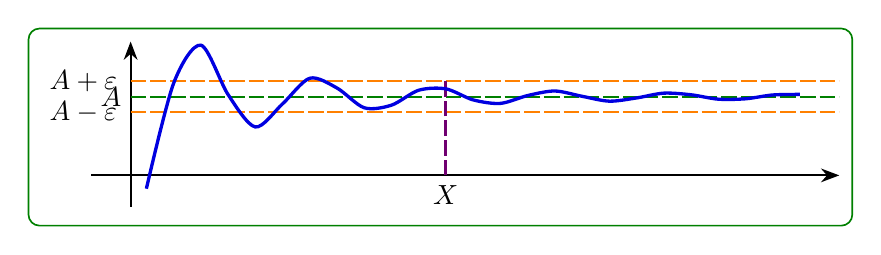
\begin{tikzpicture}[framed]
			\draw[cstaxis] (-0.5,0)--(9,0);
			\draw[cstaxis] (0,-0.4)--(0,1.7);
			\begin{scope}[visible on=<1>]
				\draw[cstdash,fourth] (0,1)--(9,1);
				\draw (-0.25,1) node {$A$};
			\end{scope}
			\begin{scope}[visible on=<2->]
				\draw[cstdash,fifth] (0,1.2)--(9,1.2);
				\draw[cstdash,fifth] (0,0.8)--(9,0.8);
				\draw[cstdash,third] (4,0)--(4,1.2);
				\draw (-0.6,1.2) node {$A+\varepsilon$};
				\draw (-0.6,0.8) node {$A-\varepsilon$};
				\draw (4,-0.25) node {$X$};
			\end{scope}
			\draw[cstcurve,main,smooth,domain=1.2:9.5] plot({\x-1},{1+3*sin(\x*240)/(1+\x*\x)});
		\end{tikzpicture}
	\end{center}

	\onslide<+->\onslide<+->
	仿造上述定义, 我们有:
	\onslide<+->
	\begin{definition}
		设 $x<-M$ 时函数 $f(x)$ 有定义.
		\onslide<+->{如果存在常数 $A$ 满足:
			\begin{center}
				\alert{$\forall\varepsilon>0, \exists X$ 使得当 $x<-X$ 时, 有 $\abs{f(x)-A}<\varepsilon$,}
			\end{center}
		}\onslide<+->{则称 $A$ 为 \emph{$f(x)$ 当 $x\ra-\infty$ 时的极限}, 记为 \emph{$\lim\limits_{x\ra-\infty}f(x)=A$}.}
	\end{definition}
\end{frame}


\begin{frame}{函数在 $\infty$ 的极限}
	\onslide<+->
	\begin{definition}
		设 $|x|>M$ 时函数 $f(x)$ 有定义.
		\onslide<+->{如果存在常数 $A$ 满足:
			\begin{center}
				\alert{$\forall\varepsilon>0, \exists X$ 使得当 $|x|>X$ 时, 有 $\abs{f(x)-A}<\varepsilon$,}
			\end{center}
		}\onslide<+->{则称 $A$ 为 \emph{$f(x)$ 当 $x\ra\infty$ 时的极限}, 记为 \emph{$\lim\limits_{x\ra\infty}f(x)=A$}.}
	\end{definition}
	\onslide<+->
	注意, 函数极限中需要分清 $x\ra\infty, x\ra+\infty, x\ra-\infty$, 而数列情形只有 $n\ra\infty$, 因为 $n$ 是正整数.

	\onslide<+->
	类似于数列极限与子数列极限的关系, 我们有
	\onslide<+->
	\begin{theorem}
		$\lim\limits_{x\ra\infty}f(x)=A \iff \lim\limits_{x\ra+\infty}f(x)=\lim\limits_{x\ra-\infty}f(x)=A$.
	\end{theorem}
\end{frame}


\begin{frame}{函数在一点的极限}
	\onslide<+->
	类似地, 当 $x$ 越来越接近 $x_0$ 时,
	\onslide<+->
	如果函数值 $f(x)$ 越来越接近常数 $A$, 则 $A$ 就是 $x\to x_0$ 时的极限.
	\onslide<+->
	\begin{center}
		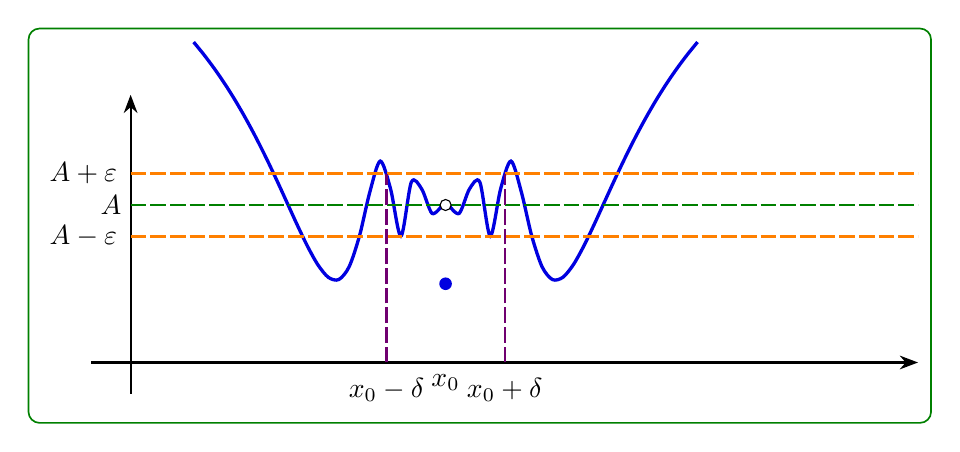
\begin{tikzpicture}[framed]
			\draw[cstaxis] (-0.5,0)--(10,0);
			\draw[cstaxis] (0,-0.4)--(0,3.4);
			\draw[cstcurve,main,smooth,domain=0.02:1.6] plot({4+2*\x},{2+1.4*\x*sin(1/\x*180)});
			\draw[cstcurve,main,smooth,domain=0.02:1.6] plot({4-2*\x},{2+1.4*\x*sin(1/\x*180)});
			\begin{scope}[visible on=<3>]
				\draw[cstdash,fourth] (0,2)--(10,2);
				\draw (-0.25,2) node {$A$};
				\draw (4,-0.25) node {$x_0$};
			\end{scope}
			\begin{scope}[visible on=<4->]
				\draw[cstdash,fifth] (0,2.4)--(10,2.4);
				\draw[cstdash,fifth] (0,1.6)--(10,1.6);
				\draw[cstdash,third] (3.25,0)--(3.25,2.4);
				\draw[cstdash,third] (4.75,0)--(4.75,2.4);
				\draw (-0.6,2.4) node {$A+\varepsilon$};
				\draw (-0.6,1.6) node {$A-\varepsilon$};
				\draw (4.75,-0.35) node {$x_0+\delta$};
				\draw (3.25,-0.35) node {$x_0-\delta$};
			\end{scope}
			\filldraw[cstdote] (4,2) circle;
			\fill[cstdot,main] (4,1) circle;
		\end{tikzpicture}
	\end{center}
\end{frame}


\begin{frame}{函数在一点的极限}
	\onslide<+->
	为了陈述方便, 我们引入去心邻域的概念.
	\onslide<+->
	\begin{definition}
	设 $\delta>0$. $x_0$ 的\emph{去心 $\delta$ 邻域}是指
		\[\Uc(x_0,\delta)=\set{x: 0<|x-x_0|<\delta}=(x_0-\delta,x_0)\cup(x_0,x_0+\delta).\]
	\end{definition}
	\onslide<+->
	\begin{definition}
		设函数 $f(x)$ 在 $x_0$ 的某个去心邻域内有定义.
		\onslide<+->{如果存在常数 $A$ 满足
		\begin{center}
			\alert{$\forall\varepsilon>0, \exists\delta>0$ 使得当 $x\in\Uc(x_0,\delta)$ 时, 有 $|f(x)-A|<\varepsilon$,}
		\end{center}
		}\onslide<+->{则称 $A$ 为 $f(x)$ 当 $x\ra x_0$ 时的极限, 记为 $\lim\limits_{x\ra x_0}f(x)=A$ 或 $f(x)\ra A(x\ra x_0)$.
		}\onslide<+->{\begin{tikzpicture}[overlay]
			\draw[semithick,third] (1.8,1.2) rectangle (12.4,1.9);
			\draw (13.4,1.55) node[third] {$\varepsilon$-$\delta$ 语言};
		\end{tikzpicture}}
	\end{definition}
\end{frame}


\begin{frame}{函数在一点的单侧极限}
	\onslide<+->
	类似地可以定义单侧极限:
	\onslide<+->
	\begin{align*}
		 \lim\limits_{x\ra x_0^+}f(x)=A&\iff\alert{\forall\varepsilon>0, \exists\delta>0\;\text{使得当}\;x\in(x_0,x_0+\delta)\;\text{时, 有}\;|f(x)-A|<\varepsilon}.\\
		\lim\limits_{x\ra x_0^-}f(x)=A&\iff\alert{\forall\varepsilon>0, \exists\delta>0\;\text{使得当}\;x\in(x_0-\delta,x_0)\;\text{时, 有}\;|f(x)-A|<\varepsilon}.
	\end{align*}
	\onslide<+->
	同样地, 我们有:
	\begin{theorem}
		$\lim\limits_{x\ra x_0}f(x)=A\iff\lim\limits_{x\ra x_0^+}f(x)=\lim\limits_{x\ra x_0^-}f(x)=A$.
	\end{theorem}
	\onslide<+->
	为了简便, 我们记 \alert{$f(x_0^+)=\lim\limits_{x\ra x_0^+}f(x)$, $f(x_0^-)=\lim\limits_{x\ra x_0^-}f(x)$}.
	\onslide<+->
	注意它们和 $f(x_0)$ 并无关系, $f$ 甚至可以在 $x_0$ 处无定义.
\end{frame}


\subsection{函数极限的证明}
\begin{frame}{例题: 函数在无穷远的极限}
	\onslide<+->
	\begin{example}
		证明 $\lim\limits_{x\ra\infty}\dfrac1x=0$.
	\end{example}
	\onslide<+->
	\begin{analysis}
		和数列极限类似, 这种问题的证明通常也分为两步:
		\begin{itemize}
			\item 估计 $|f(x)-A|$, 得到它和 $|x-x_0|<\delta$ 或 $|x|>X$ 的不等式关系. 从而求得 $\delta$ 或 $X$. 这个过程中可以进行适当的放缩.
			\item 将 $\delta$ 或 $X$ 代入极限的定义中.
		\end{itemize}
		\onslide<+->{对于本题, 从 $\Bigl|\dfrac1x-0\Bigr|<\varepsilon$ 解得 $|x|>\dfrac1\varepsilon$.}
	\end{analysis}
	\onslide<+->
	\begin{proof}
		$\forall\varepsilon>0$, 令 $X=\dfrac1\varepsilon$.
		\onslide<+->{当 $|x|>X$ 时, 有 $\Bigl|\dfrac1x-0\Bigr|=\dfrac1{|x|}<\varepsilon$.
		}\onslide<+->{所以 $\lim\limits_{x\ra\infty}\dfrac1x=0$.\qedhere}
	\end{proof}
\end{frame}


\begin{frame}{例题: 函数在无穷远的单侧极限}
	\onslide<+->
	\begin{example}
		证明 $a>1$ 时, $\lim\limits_{x\ra-\infty}a^x=0$.
	\end{example}
	\onslide<+->
	\begin{analysis}
		由于 $a>1$ 时, $\log_ax$ 是单调递增的.
		\onslide<+->{因此 $|a^x-0|=a^x<\varepsilon \iff x<\log_a \varepsilon$.}
	\end{analysis}
	\onslide<+->
	\begin{proof}
		$\forall\varepsilon>0$, 令 $X=-\log_a\varepsilon$.
		\onslide<+->{当 $x<-X$ 时, 有 $|a^x-0|=a^x<\varepsilon$.}
		
		\onslide<+->{所以 $\lim\limits_{x\ra-\infty}a^x=0$.\qedhere}
	\end{proof}
\end{frame}


\begin{frame}{例题: 函数在一点的极限}\small
	\onslide<+->
	\begin{example}
		证明 $\lim\limits_{x\ra x_0}(ax+b)=ax_0+b$.
	\end{example}
	\onslide<+->
	\begin{analysis}
		$|(ax+b)-(ax_0+b)|=a\cdot|x-x_0|<\varepsilon$, 因此我们可以取 $\delta=\varepsilon/a$.
		\onslide<+->{注意我们需要单独考虑 $a=0$ 的情形.}
	\end{analysis}
	\onslide<+->
	\begin{proof*}
		我们有 $|(ax+b)-(ax_0+b)|=a\cdot|x-x_0|$.
		\onslide<+->{如果 $a=0$, $\forall\varepsilon>0$, 令 $\delta=1$.
		}\onslide<+->{当 $0<|x-x_0|<\delta$ 时, 有 $|(ax+b)-(ax_0+b)|=0<\varepsilon$.}

		\onslide<+->{如果 $a\neq 0$, $\forall\varepsilon>0$, 令 $\delta=\dfrac\varepsilon a$.
		}\onslide<+->{当 $0<|x-x_0|<\delta$ 时, 有
			\[|(ax+b)-(ax_0+b)|=a\cdot|x-x_0|<a\delta=\varepsilon.\]
		}\onslide<+->{所以 $\lim\limits_{x\ra x_0}(ax+b)=ax_0+b$.\qedhere}
	\end{proof*}
\end{frame}


\begin{frame}{例题: 线性函数在一点的极限}
	\onslide<+->
	\begin{example}
		证明 $\lim\limits_{x\ra x_0}\sin x=\sin x_0$.
	\end{example}
	\onslide<+->
	与三角函数有关的放缩往往要用到和差化积公式
	\[\sin x-\sin y=2\sin\frac{x-y}2\cos\frac{x+y}2,\quad
	\cos x-\cos y=-2\sin\frac{x+y}2\sin\frac{x-y}2,\]
	然后将不含 $x-x_0$ 的项放缩到 $1$;
	\onslide<+->
	以及三角函数基本不等式
	\[\left|\sin x\right|\le|x|, \forall x;\qquad|x|\le\left|\tan x\right|, \forall x \in\bigl(-\frac\pi2,\frac\pi2\bigr).\]
\end{frame}


\begin{frame}{例题: 三角函数在一点的极限}
	\onslide<+->
	\begin{proof*}
		我们有
		\[\left|\sin x-\sin x_0\right|=\Bigl|2\sin\frac{x-x_0}2\cos\frac{x+x_0}2\Bigr|
			\le2\Bigl|\sin\frac{x-x_0}2\Bigr|
			\le2\Bigl|\frac{x-x_0}2\Bigr|=|x-x_0|.\]

		\onslide<+->{$\forall\varepsilon>0$, 令 $\delta=\varepsilon$.
		}\onslide<+->{当 $0<|x-x_0|<\delta$ 时, 有
		\[\left|\sin x-\sin x_0\right|\le|x-x_0|<\delta=\varepsilon.\]
		}\onslide<+->{所以 $\lim\limits_{x\ra x_0}\sin x=\sin x_0$.\qedhere}
	\end{proof*}
\end{frame}


\begin{frame}{例题: 函数在无穷远的极限}
	\onslide<+->
	\begin{example}
		证明 $\lim\limits_{x\ra\infty}\arctan x$ 不存在.
	\end{example}
	\onslide<+->
	\begin{analysis*}
		从图像上可以看出 $\lim\limits_{x\ra\pm\infty}\arctan x=\pm\dfrac\pi2$.

		\onslide<+->{我们想要使用 $|x|$ 来控制 $\Bigl|\arctan x-\dfrac\pi2\Bigr|$, 不过这个形式不容易估计.
		}\onslide<+->{令 $t=\dfrac\pi2-\arctan x$, 则问题变成了 $|x|=\Bigl|\tan\Bigl(\dfrac\pi2-t\Bigr)\Bigr|=\dfrac1{\left|\tan t\right|}$ 和 $|t|$ 的关系.
		}\onslide<+->{而我们有 $|t|\le |\tan t|$.}

		\onslide<+->{我们还需要估计 $t$ 的范围.
		}\onslide<+->{由于我们考虑的是 $x\ra+\infty$, 不妨设 $x>0$,
		}\onslide<+->{那么
		\[\arctan x \in\Bigl(0,\frac\pi2\Bigr),\qquad t=\frac\pi2-\arctan x\in\Bigl(0,\frac\pi2\Bigr).\]}
		\vspace{-\baselineskip}
	\end{analysis*}
\end{frame}


\begin{frame}{例题: 函数在无穷远的极限}
	\begin{proof*}
		我们来证明 $\lim\limits_{x\ra+\infty}\arctan x=\dfrac\pi2$.
		\onslide<+->{当 $x>0$ 时, $0<\dfrac\pi2-\arctan x<\dfrac\pi2$.
		}\onslide<+->{因此
			\[\Bigl|\frac\pi2-\arctan x\Bigr|
			\le\Bigl|\tan\Bigl(\frac\pi2-\arctan x\Bigr)\Bigr|
			=\frac1{\left|\tan(\arctan x)\right|}=\frac1{|x|}.\]
		}\onslide<+->{$\forall\varepsilon>0$, 令 $X=\dfrac1\varepsilon>0$.
		}\onslide<+->{当 $x>X$ 时, 有
		\[\Bigl|\frac\pi2-\arctan x\Bigr|\le\frac1{|x|}<\frac1X=\varepsilon.\]
		}\onslide<+->{所以 $\lim\limits_{x\ra+\infty}\arctan x=\dfrac\pi2$.}

		\onslide<+->{类似可证, $\lim\limits_{x\ra-\infty}\arctan x=-\dfrac\pi2$.
		}\onslide<+->{因此 $\lim\limits_{x\ra\infty}\arctan x$ 不存在.\qedhere}
	\end{proof*}
\end{frame}


\begin{frame}{例题: 有理函数在一点的极限}\small
	\beqskip{2pt}
	\onslide<+->
	\begin{example}
		证明 $\lim\limits_{x\ra2}\dfrac{x^2-4}{x-2}=4$.
	\end{example}
	\onslide<+->
	\begin{analysis}
		这种极限是 $\dfrac fg$ 型, 其中 $f\ra0, g\ra0$.
		\onslide<+->{我们称之为 \emph{$\dfrac00$ 型不定式}.
		}\onslide<+->{它的极限可能存在, 可能不存在.
		}\onslide<+->{这种一般要去掉公因式, 将其变为定式.}
	\end{analysis}
	\onslide<+->
	\begin{proof}
		$\displaystyle \biggl|\frac{x^2-4}{x-2}-4\biggr|=|x+2-4|=|x-2|$.
		\onslide<+->{$\forall\varepsilon>0$, 令 $\delta=\varepsilon$.
		}\onslide<+->{当 $0<|x-2|<\delta$ 时, 有
		\[\biggl|\frac{x^2-4}{x-2}-4\biggr|=|x-2|<\varepsilon.\]
		}\onslide<+->{所以 $\lim\limits_{x\ra2}\dfrac{x^2-4}{x-2}=4$.\qedhere}
	\end{proof}
	\endgroup
\end{frame}


\begin{frame}{例题: 分段函数求待定参数}
	\onslide<+->
	\begin{example}
		如果函数 $f(x)=\begin{cases}
			a\sin x,&x<\pi/2;\\
			x+b,&x>\pi/2
		\end{cases}$ 满足 $\lim\limits_{x\ra\pi/2}f(x)=1$, 求 $a,b$.
	\end{example}
	\onslide<+->
	\begin{analysis*}
		本题是典型的由分段函数性质求待定参数的问题, 我们后续会经常遇到.
		\onslide<+->{由于一点处极限等价于两侧极限都存在且为 $1$, 因此我们会得到两个等式, 从而可以解出两个未知参数.}

		\onslide<+->{由于 $f(x)$ 的两个分段都是我们已经求过极限的函数, 因此我们可以直接用前面已经证明的结论.}
	\end{analysis*}
	\onslide<+->
	\begin{solution}
		由于 $\displaystyle f\Bigl[\bigl(\frac\pi2\bigr)^+\Bigr]=\frac\pi2+b,\ 
		f\Bigl[\bigl(\frac\pi2\bigr)^-\Bigr]=a\sin\frac\pi2=a$,
		\onslide<+->{因此 $a=1, b=1-\dfrac\pi2$.}
	\end{solution}
\end{frame}


\begin{frame}{例题: 取整函数的极限}
	\beqskip{7pt}
	\onslide<+->
	\begin{example}
		对于哪些 $x_0$, $\lim\limits_{x\ra x_0}[x]$ 存在.
	\end{example}
	\onslide<+->
	\begin{analysis*}
		与 $[x]$ 有关的问题往往需要用到两个不等式
		\begin{center}
			\alert{$[x]\le x<x+1$} 或 \alert{$x-1<[x]\le x$}.
		\end{center}

		\onslide<+->{从 $[x]$ 的图像上可以看出 $x_0\in\BZ$ 时左右极限不相等, 从而极限不存在.
		}\onslide<+->{解答时, 我们取 $x_0$ 的 $\delta=1/2$ 邻域, 则在这个邻域的左右各自半边内, $[x]$ 是常值函数, 从而得到单侧极限.}

		\onslide<+->{当 $x_0\notin \BZ$ 时, 我们同样希望取一个小邻域使得 $[x]$ 是常值函数.
		}\onslide<+->{这需要 $\delta$ 不超过 $x_0$ 和两边的最近的整数的距离.
		}\onslide<+->{所以
		\[\delta=\min\set{x_0-[x_0], [x_0]+1-x_0}.\]}
		\vspace{-\baselineskip}
	\end{analysis*}
	\endgroup
\end{frame}


\begin{frame}{例题: 取整函数的极限}
	\onslide<+->
	\begin{solution*}
		如果 $x_0\in\BZ$, 则
		\begin{itemize}
			\item 当 $x\in(x_0, x_0+1/2)$ 时, $[x]=x_0$, 所以 $\lim\limits_{	x\ra x_0^+}[x]=x_0$;
			\item 当 $x\in(x_0-1/2, x_0)$ 时, $[x]=x_0-1$, 所以 $\lim\limits_{	x\ra x_0^-}[x]=x_0-1$.
		\end{itemize}
		\onslide<+->{因此 $\lim\limits_{x\ra x_0}[x]$ 不存在.}

		\onslide<+->{如果 $x_0\notin\BZ$, 令 $\delta=\min\set{x_0-[x_0], [x_0]+1-x_0}>0$.
		}\onslide<+->{name 
		\[[x_0]\le x_0-\delta<x_0+\delta\le[x_0]+1.\]
		}\onslide<+->{当 $0<|x-x_0|<\delta$ 时, 有 $x_0-\delta<x<x_0+\delta$,
		}\onslide<+->{从而 $[x_0]<x<[x_0]+1$, $[x]=x_0$.
		}\onslide<+->{因此 $\lim\limits_{x\ra x_0}[x]=x_0$.}

		\onslide<+->{故当且仅当 $x_0\notin\BZ$ 时, $\lim\limits_{x\ra x_0}[x]$ 存在.}
	\end{solution*}
\end{frame}

\section{初等函数}

\subsection{指数函数}

\begin{frame}{指数函数}
	\onslide<+->
	我们将实变函数中的初等函数推广到复变函数.
	\onslide<+->
	多项式函数和有理函数的解析性质已经介绍过, 这里不再重复.
	\onslide<+->
	现在我们来定义指数函数.

	\onslide<+->
	指数函数有多种等价的定义方式:
	\begin{enumerate}
		\item $\exp z=\ee^x(\cos y+\ii\sin y)$ (欧拉恒等式);
		\item $\exp z=\liml_{n\to\infty}\Bigl(1+\dfrac zn\Bigr)^n$ (极限定义);
		\item $\exp z=1+z+\dfrac{z^2}{2!}+\dfrac{z^3}{3!}+\cdots
		=\liml_{n\to\infty}\sum\limits_{k=0}^n\dfrac{z^k}{k!}$ (级数定义);
		\item $\exp z$ 是唯一的一个处处解析的函数, 使得当 $z=x\in\BR$ 时, $\exp z=\ee^x$ ($\ee^x$ 的解析延拓).
	\end{enumerate}
\end{frame}


\begin{frame}{指数函数与欧拉恒等式}
	\onslide<+->
	有些人会从 $\ee^x,\cos x,\sin x$ 的泰勒展开
	\begin{align*}
		\ee^x&=1+x+\frac{x^2}{2!}+\frac{x^3}{3!}+\cdots\\
		\cos x&=1-\frac{x^2}{2!}+\frac{x^4}{4!}+\cdots\\
		\sin x&=x-\frac{x^3}{3!}+\frac{x^5}{5!}\cdots
	\end{align*}
	形式地带入得到欧拉恒等式 $\ee^{\ii x}=\cos x+\ii\sin x$.
	\onslide<+->
	事实上我们可以把它当做复指数函数的定义, 而不是欧拉恒等式的证明.
	\onslide<+->
	我们将在第四章说明\enumnum1、\enumnum3和\enumnum4是等价的.
\end{frame}



\begin{frame}{指数函数的定义}
	\onslide<+->
	我们来证明\enumnum1和\enumnum2等价.
	\onslide<+->
	\begin{align*}
		\lim_{n\to\infty}\Bigabs{1+\frac zn}^n
		&=\lim_{n\to\infty}\Bigl(1+\frac{2x}n+\frac{x^2+y^2}{n^2}\Bigr)^{\frac n2}\quad
		\visible<+->{(1^\infty\ \text{型不定式})}\\
		&\visible<+->{=\exp\left[\lim_{n\to\infty}\frac n2
		\Bigl(\frac{2x}n+\frac{x^2+y^2}{n^2}\Bigr)\right]=\ee^x.}
	\end{align*}
	\onslide<+->
	不妨设 $n>\abs{z}$, 这样 $1+\dfrac zn$ 落在右半平面,
	\onslide<+->
	\[
		\lim_{n\to\infty} n\arg{\Bigl(1+\frac zn\Bigr)}
		=\lim_{n\to\infty} n\arctan \frac y{n+x}
		\visible<+->{=\lim_{n\to\infty}\frac{ny}{n+x}=y.}
	\]
	\bigdel
	\onslide<+->
	故 $\exp z=\ee^x(\cos y+\ii\sin y)$.
\end{frame}


\begin{frame}{指数函数的性质}
	\onslide<+->
	\begin{definition*}[][指数函数]
	\[
		\exp z:=\ee^x(\cos y+\ii\sin y).
	\]
	\end{definition*}
	\onslide<+->
	为了方便, 我们也记 $\emphm{\ee^z=\exp z}$.
	\onslide<+->
	指数函数有如下性质:
	\begin{itemize}\bf
		\item $\exp z$ 处处解析, 且 $(\exp z)'=\exp z$.
		\item $\exp z\neq 0$.
		\item $\exp(z_1+z_2)=\exp z_1\cdot \exp z_2$.
		\item $\exp(z+2k\pi\ii)=\exp z$, 即 $\exp z$ 周期为 $2\pi\ii$.
		\item $\exp z_1=\exp z_2$ 当且仅当 $z_1=z_2+2k\pi\ii,k\in\BZ$.
		\item 指数函数将直线族 $\Re z=c$ 映为圆周族 $\abs{w}=\ee^c$, 将直线族 $\Im z=c$ 映为射线族 $\Arg w=c$.
	\end{itemize}
\end{frame}


\begin{frame}{指数函数的性质}
	\onslide<+->
	\begin{example}
		计算函数 $f(z)=\exp(z/6)$ 的周期.
	\end{example}

	\onslide<+->
	\begin{solution}
		设 $f(z_1)=f(z_2)$, 则 $\ee^{z_1/6}=\ee^{z_2/6}$.
		\onslide<+->{%
			因此存在 $k\in\BZ$ 使得
			\[
				\frac{z_1}6=\frac{z_2}6+2k\pi\ii,
			\]
		}\onslide<+->{%
			从而 $z_1-z_2=12k\pi\ii$.
		}\onslide<+->{%
			所以 $f(z)$ 的周期是 $12\pi\ii$.
		}
	\end{solution}

	\onslide<+->
	一般地, $\exp(az+b)$ 的周期是 $\dfrac{2\pi\ii}a$ (或写成 $-\dfrac{2\pi\ii}a$), $a\neq 0$.
\end{frame}


\subsection{对数函数}

\begin{frame}{对数函数}
	\onslide<+->
	对数函数 $\Ln z$ 定义为指数函数 $\exp z$ 的反函数.
	\onslide<+->
	为什么我们用大写的 $\Ln$ 呢? 
	\onslide<+->
	在复变函数中, 很多函数是多值函数.
	\onslide<+->
	为了便于研究, 我们会固定它的一个单值分支.
	\onslide<+->
	我们将多值的这个开头字母大写, 而对应的单值的则是开头字母小写.
	\onslide<+->
	例如 $\Arg z$ 和 $\arg z$.

	\onslide<+->
	设 $z\neq0,\ee^w=z=r\ee^{\ii\theta}=\ee^{\ln r+\ii\theta}$,
	\onslide<+->
	则
	\[w=\ln r+\ii\theta+2k\pi\ii,\quad k\in\BZ.
	\]
\end{frame}


\begin{frame}{对数函数及其主值}
	\onslide<+->
	\begin{definition*}{对数函数}
		\begin{enumerate}
			\item 定义\emph{对数函数}
			\[
				\Ln z=\ln\abs{z}+\ii\Arg z.
			\]
			它是一个多值函数.
			\item 定义\emph{对数函数主值}
			\[
				\ln z=\ln\abs{z}+\ii\arg z.
			\]
			\bigdel
		\end{enumerate}
	\end{definition*}

	\onslide<+->
	对于每一个整数 $k$, $\ln z+2k\pi\ii$ 都给出了 $\Ln z$ 的一个单值分支.
	\onslide<+->
	特别地, 当 $z=x>0$ 是正实数时, $\ln z$ 就是实变的对数函数.
\end{frame}


\begin{frame}{例题: 对数函数的计算}
	\onslide<+->
	\begin{example}
		求 $\Ln 2,\Ln(-1)$ 以及它们的主值.
	\end{example}

	\onslide<+->
	\begin{solution}
		\begin{enumerate}
			\item
			\[
				\Ln2=\ln2+2k\pi\ii, k\in\BZ,
			\]
			\onslide<+->{%
				主值为 $\ln 2$.
			}
			\item
			\[
				\Ln(-1)=\ln1+\ii\Arg(-1)=(2k+1)\pi\ii, k\in\BZ,
			\]
			\onslide<+->{%
				主值为 $\pi\ii$.
			}
		\end{enumerate}
	\end{solution}
\end{frame}


\begin{frame}{例题: 对数函数的计算}
	\beqskip{5pt}
	\onslide<+->
	\begin{example}
	求 $\Ln(-2+3\ii),\Ln(3-\sqrt3 i)$.
	\end{example}

	\onslide<+->
	\begin{solution}
		\begin{enumerate}
			\item
			\begin{align*}
				\Ln(-2+3\ii)&=\ln\abs{-2+3\ii}+\ii\Arg(-2+3\ii)\\
				&\visible<+->{=\frac 12\ln 13+\Bigl(-\arctan\frac 32+\pi+2k\pi\Bigr)\ii,\quad k\in\BZ.}
			\end{align*}
			\item
			\begin{align*}
				\Ln(3-\sqrt3\ii)&=\ln\abs{3+\sqrt 3\ii}+\ii\Arg(3-\sqrt 3\ii)\\
				&\visible<+->{=\ln 2\sqrt 3+\Bigl(-\frac\pi6+2k\pi\Bigr)\ii
				=\ln 2\sqrt 3+\Bigl(2k-\frac16\Bigr)\pi\ii,\quad k\in\BZ.}
			\end{align*}
		\end{enumerate}
		\vspace{-.5\baselineskip}
	\end{solution}
	\endgroup
\end{frame}


\begin{frame}{例题: 对数函数的计算}
	\onslide<+->
	\begin{example}
		解方程 $\ee^z-1-\sqrt 3\ii=0$.
	\end{example}

	\onslide<+->
	\begin{solution}
		由于 $1+\sqrt 3 i=2\ee^{\frac{\pi\ii}3}$,
		\onslide<+->{%
			因此
			\[
				z=\Ln(1+\sqrt 3\ii)=\ln 2+\Bigl(2k+\frac13\Bigr)\pi\ii,\quad k\in\BZ.
			\]
		}\bigdel
	\end{solution}

	\onslide<+->
	\begin{exercise}
		求 $\ln(-1-\sqrt3\ii)=$\fillblankframe[2cm][3mm]{$\ln 2-\dfrac{2\pi\ii}3$}.
	\end{exercise}
\end{frame}


\begin{frame}{对数函数的性质}
	\onslide<+->
	对数函数与其主值的关系是
	\[
		\emphn{\Ln z=\ln z+\Ln 1=\ln z+2k\pi\ii,\quad k\in\BZ}.
	\]

	\onslide<+->
	根据辐角以及辐角主值的相应等式, 我们有
	\[
		\Ln(z_1\cdot z_2)=\Ln z_1+\Ln z_2,\quad
		\Ln\frac{z_1}{z_2}=\Ln z_1-\Ln z_2,
	\]
	\[
		\Ln \sqrt[n]z=\dfrac1n\Ln z.
	\]
	\onslide<+->
	而当 $\abs{n}\ge 2$ 时, \alert{$\Ln z^n=n\Ln z$ 不成立}.
	\onslide<+->
	以上等式换成 $\ln z$ 均未必成立.
\end{frame}


\begin{frame}{对数函数的导数}
\beqskip{1pt}
	\onslide<+->
	设 $x$ 是正实数, 
	\onslide<+->
	则
	\[
		\ln (-x)=\ln x+\pi\ii,\quad
		\lim_{y\to0^-}\ln (-x+y\ii)=\ln x-\pi\ii,
	\]
	\onslide<+->
	因此 $\ln z$ 在负实轴和零处不连续.

	\onslide<+->
	而在其它地方 $-\pi<\arg z<\pi$, $\ln z$ 是 $\ee^z$ 在区域 $-\pi<\Im z<\pi$ 上的单值反函数, 
	\onslide<+->
	从而
	\alert{$(\ln z)'=\dfrac 1z$},
	\alert{$\ln z$ 在除负实轴和零处的区域解析}.

	\onslide<+->
	也可以通过C-R方程来得到 $\ln z$ 的解析性和导数: 当 $x>0$ 时,
	\[
		\ln z=\half \ln(x^2+y^2)+\ii\arctan \frac yx,
	\]
	\onslide<+->
	\[
		u_x=v_y=\frac x{x^2+y^2},\qquad v_x=-u_y=-\frac y{x^2+y^2},
	\]
	\[
		(\ln z)'=\frac{x-yi}{x^2+y^2}=\frac 1z.
	\]
	其它情形可取虚部为 $\arccot\dfrac xy$ 或 $\arccot\dfrac xy-\pi$ 类似证明.
\endgroup
\end{frame}


\subsection{幂函数}

\begin{frame}{幂函数的性质: $a$ 为整数时}
	\onslide<+->
	\begin{definition*}[][幂函数]
		\begin{enumerate}
			\item 设 $a\neq 0$, $z\neq 0$, 定义\emph{幂函数}
			\[
				w=z^a=\ee^{a\Ln z}
				=\exp\bigl[a\ln\abs{z}+\ii a(\arg z+2k\pi)\bigr],\quad k\in\BZ.
			\]
			\item \emph{幂函数的主值}为
			\[
				w=\ee^{a\ln z}=\exp\bigl(a\ln\abs{z}+\ii a\arg z\bigr).
			\]
		\end{enumerate}
		\bigdel
	\end{definition*}
	\onslide<+->
	根据 $a$ 的不同, 这个函数有着不同的性质.

	\onslide<+->
	当 $a$ 为整数时, 因为 $\ee^{2ak\pi\ii}=1$, 所以 $w=z^a$ 是单值的.
	\onslide<+->
	此时 $z^a$ 就是我们之前定义的乘幂.

	\onslide<+->
	当 $a$ 是非负整数时, $z^a$ 在复平面上解析;
	\onslide<+->
	当 $a$ 是负整数时, $z^a$ 在 $\BC-\{0\}$ 上解析.
\end{frame}


\begin{frame}{幂函数的性质: $a$ 为分数时}
	\onslide<+->
	当 $a=\dfrac pq$ 为分数, $p,q$ 为互质的整数且 $q>1$ 时,
	\onslide<+->
	\[
		z^{\frac pq}=\abs{z}^{\frac pq}\exp\left[\frac{\ii p(\arg z+2k\pi)}q\right],\quad k=0,1,\dots,q-1
	\]
	具有 $q$ 个值.
	\onslide<+->
	去掉负实轴和 $0$ 之后, 它的主值 $w=\exp(a\ln z)$ 是处处解析的.
	\onslide<+->
	事实上它就是 $\sqrt[q]{z^p}=(\sqrt[q]z)^p$.
	\onslide<+->
	\begin{center}
		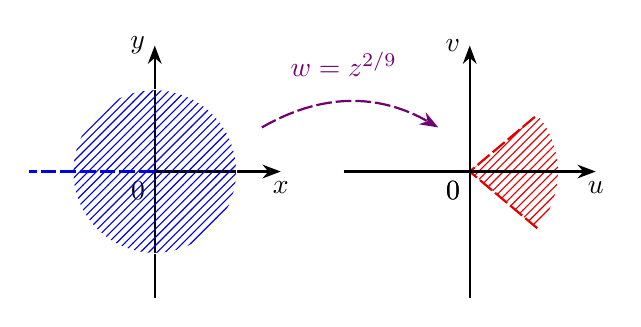
\begin{tikzpicture}[scale=.8]
			\coordinate [label=below left:{$0$}] (O) at (0,0);
			\coordinate [label=below:{$x$}] (X) at (2,0);
			\coordinate [label=left:{$y$}] (Y) at (0,2);
			\draw[cstaxis] (O)--(X);
			\draw[cstaxis] (0,-2)--(Y);
			\draw[draw=white,cstfille1] (O) circle (1.3);
			\draw[cstdash,main] (0,0)--(-2,0);
			\draw[cstdash,cstra,third] (1.7,.7)to [bend left] (4.5,.7);
			\draw (3,1.7) node[third] {$w=z^{2/9}$};
			\begin{scope}[xshift=5cm]
				\coordinate [label=below left:{$0$}] (O) at (0,0);
				\fill[cstfille2,pattern color=second] (O)--({1.4*cos(40)},{1.4*sin(40)}) arc (40:-40:1.4)--cycle;
				\draw[cstdash,second] ({1.4*cos(40)},{-1.4*sin(40)})--(0,0)--({1.4*cos(40)},{1.4*sin(40)});
				\coordinate [label=below left:{$0$}] (O) at (0,0);
				\coordinate [label=below:{$u$}] (X) at (2,0);
				\coordinate [label=left:{$v$}] (Y) at (0,2);
				\draw[cstaxis] (-2,0)--(X);
				\draw[cstaxis] (0,-2)--(Y);
			\end{scope}
		\end{tikzpicture}
	\end{center}
\end{frame}


\begin{frame}{幂函数的性质: $a$ 为其他情形}
\onslide<+->
	对于其它的 $a$, $z^a$ 具有无穷多个值.
	\onslide<+->
	这是因为此时当 $k\neq0$ 时, $2k\pi a \ii$ 不可能是 $2\pi\ii$ 的整数倍. 
	\onslide<+->
	从而不同的 $k$ 得到的是不同的值.
	\onslide<+->
	去掉负实轴和 $0$ 之后,
	\onslide<+->
	它的主值 $w=\exp(a\ln z)$ 也是处处解析的.
	\onslide<+->
	\begin{center}
		\arrayrulecolor{second}
		\begin{tabular}{cccc} \toprule
			$a$& $z^a$ 的值& $z^a$ 的解析区域\\ \midrule
			&&$n\ge0$ 时处处解析\\
			\multirow{-2}*{整数 $n$}&\multirow{-2}*{单值}&$n<0$ 时除零点外解析\\ \midrule
			分数 $p/q$&$q$ 值&除负实轴和零点外解析\\ \midrule
			无理数或虚数&无穷多值&除负实轴和零点外解析\\ \bottomrule
		\end{tabular}
	\end{center}
\end{frame}


\begin{frame}{典型例题: 幂函数的计算}
	\onslide<+->
	\begin{example}
		求 $1^{\sqrt 2}$ 和 $\ii^\ii$.
	\end{example}
	\onslide<+->
	\begin{solution}
		\[
			1^{\sqrt2}=\ee^{\sqrt2\Ln1}
			\visible<+->{=\ee^{\sqrt 2\cdot 2k\pi\ii}}
			\visible<+->{=\cos(2\sqrt 2k\pi)+\ii\sin(2\sqrt 2k\pi), k\in\BZ.}
		\]
		\onslide<+->{%
			\[
				\ii^\ii=\ee^{\ii\Ln \ii}
				\visible<+->{=\exp\left[\ii\cdot\Bigl(2k+\half\Bigr)\pi\ii\right]}
				\visible<+->{=\exp\Bigl(-2k\pi-\half\pi\Bigr), k\in\BZ.}
			\]
		}\bigdel
	\end{solution}
	\onslide<+->
	\begin{exercise}
		$3^\ii$ 的辐角主值是\fillblankframe{$\ln 3$}.
	\end{exercise}
\end{frame}


\begin{frame}{幂函数的性质}
	幂函数与其主值有如下关系:
	\onslide<+->
	\[
		\emphn{z^a=\ee^{a\ln z}\cdot 1^a
		=\ee^{a\ln z}\cdot \ee^{2ak\pi\ii},\quad k\in\BZ.}
	\]

	\onslide<+->
	对于幂函数的主值,
	\[
		\alertn{(z^a)'}=\Bigl(\ee^{a\ln z}\Bigr)'=\frac{a\ee^{a\ln z}}z=\alertn{az^{a-1}}.
	\]

	\onslide<+->
	一般而言, $z^a\cdot z^b=z^{a+b}$ 和 $(z^a)^b=z^{ab}$ 都是不成立的.

	\onslide<+->
	最后, 注意 $\ee^a$ 作为指数函数 $f(z)=\ee^z$ 在 $a$ 处的值和作为 $g(z)=z^a$ 在 $e$ 处的值是\alert{不同}的.
	\onslide<+->
	因为后者在 $a\not\in\BZ$ 时总是多值的.
	\onslide<+->
	前者实际上是后者的主值.
	\onslide<+->
	为避免混淆, 以后我们总\alert{默认 $\ee^a$ 表示指数函数 $\exp a$}.
\end{frame}


\subsection{三角函数和反三角函数}

\begin{frame}{三角函数的定义}
	\onslide<+->
	我们知道
	\[
		\cos x=\frac{\ee^{\ii x}+\ee^{-\ii x}}2,\quad
		\sin x=\frac{\ee^{\ii x}-\ee^{-\ii x}}{2\ii}
	\]
	对于任意实数 $x$ 成立,
	\onslide<+->
	我们将其推广到复数情形.
	\onslide<+->
	\begin{definition*}[][余弦和正弦函数]
		\[
			\cos z=\frac{\ee^{\ii z}+\ee^{-\ii z}}2,\quad
			\sin z=\frac{\ee^{\ii z}-\ee^{-\ii z}}{2\ii}.
		\]
	\end{definition*}
	\onslide<+->
	那么欧拉恒等式 \emph{$\ee^{\ii z}=\cos z+\ii\sin z$ 对任意复数 $z$ 均成立}.
\end{frame}


\begin{frame}{三角函数的性质}
	\onslide<+->
	不难得到
	\[
		\cos(\ii y)=\dfrac{\ee^y+\ee^{-y}}2,\qquad
		\visible<+->{\sin(\ii y)=\ii\dfrac{\ee^y-\ee^{-y}}2.}
	\]
	\onslide<+->
	当 $y\to\infty$ 时, $\cos(\ii y)$ 和 $\sin(\ii y)$ 都 $\to\infty$.
	\onslide<+->
	因此 \alert{$\sin z$ 和 $\cos z$ 并不有界}. 
	\onslide<+->
	这和实变情形完全不同.

	\onslide<+->
	容易看出 $\cos z$ 和 $\sin z$ 的零点都是实数.
	\onslide<+->
	于是我们可类似定义其它三角函数
	\begin{align*}
		\alertn{\tan z}&
		\alertn{=\frac{\sin z}{\cos z},z\neq\Bigl(k+\half\Bigr)\pi,}&
		\alertn{\cot z}&
		\alertn{=\frac{\cos z}{\sin z},z\neq k\pi,}\\
		\alertn{\sec z}&
		\alertn{=\frac{1}{\cos z},z\neq\Bigl(k+\half\Bigr)\pi,}&
		\alertn{\csc z}&
		\alertn{=\frac{1}{\sin z},z\neq k\pi.}
	\end{align*}
\end{frame}


\begin{frame}{三角函数的性质}
	\onslide<+->
	这些三角函数的奇偶性, 周期性和导数与实变情形类似,
	\[
		\alertn{(\cos z)'=-\sin z,\quad
		(\sin z)'=\cos z,}
	\]
	\onslide<+->
	且在定义域范围内是处处解析的.

	\onslide<+->
	三角函数的各种恒等式在复数情形也仍然成立,
	\onslide<+->
	例如
	\begin{itemize}
		\item $\cos(z_1\pm z_2)=\cos z_1 \cos z_2\mp \sin z_1 \sin z_2$,
		\item $\sin(z_1\pm z_2)=\sin z_1 \cos z_2\pm\cos z_1 \sin z_2$,
		\item $\sin^2z+\cos^2z=1$.
	\end{itemize}
\end{frame}


\begin{frame}{双曲函数}
	\onslide<+->
	类似的, 我们可以定义双曲函数:
	\onslide<+->
	\[
		\alertn{\ch z=\frac{\ee^z+\ee^{-z}}2=\cos \ii z,}
	\]
	\onslide<+->
	\[
		\alertn{\sh z=\frac{\ee^z-\ee^{-z}}2=-\ii \sin \ii z,}
	\]
	\onslide<+->
	\[
		\alertn{\tanh z=\frac{\ee^z-\ee^{-z}}{\ee^z+\ee^{-z}}
		=-\ii \tan \ii z,\quad z\neq \Bigl(k+\half\Bigr)\pi\ii.}
	\]
	\onslide<+->
	它们的奇偶性和导数与实变情形类似, 在定义域范围内是处处解析的.

	\onslide<+->
	$\ch z,\sh z$ 的周期是 $2\pi\ii$, $\tanh z$ 的周期是 $\pi\ii$.
\end{frame}


\begin{frame}{反三角函数和反双曲函数}
	\onslide<+->
	设 $z=\cos w=\dfrac{\ee^{\ii w}+\ee^{-\ii w}}2$,
	\onslide<+->
	则
	\[
		\ee^{2\ii w}-2z\ee^{\ii w}+1=0,\quad
		\visible<+->{\ee^{\ii w}=z+\sqrt{z^2-1}\ \text{(双值)}.}
	\]
	\onslide<+->
	因此\emph{反余弦函数}为
	\[
		w=\Arccos z=-\ii \Ln(z+\sqrt{z^2-1}).
	\]
	\onslide<+->
	显然它是多值的.
	\onslide<+->
	同理, 我们有:
	\begin{itemize}
		\item \emph{反正弦函数} $\Arcsin z=-\ii \Ln(\ii z+\sqrt{1-z^2})$;
		\item \emph{反正切函数} $\Arctan z=-\dfrac \ii2\Ln\dfrac{1+\ii z}{1-\ii z}, z\neq \pm \ii$;
		\item \emph{反双曲余弦函数} $\Arch z=\Ln(z+\sqrt{z^2-1})$;
		\item \emph{反双曲正弦函数} $\Arsh z=\Ln(z+\sqrt{z^2+1})$;
		\item \emph{反双曲正切函数} $\Arth z=\dfrac12\Ln\dfrac{1+z}{1-z}, z\neq \pm1$.
	\end{itemize}
\end{frame}


\begin{frame}{例题: 解三角函数方程}
	\onslide<+->
	\begin{example}
		解方程 $\sin z=2$.
	\end{example}
	\onslide<+->
	\begin{solution}
	由于 $\sin z=\dfrac{\ee^{\ii z}-\ee^{-\ii z}}{2\ii}=2$,
	\onslide<+->{%
		我们有
		\[
			\ee^{2\ii z}-4\ii\ee^{\ii z}-1=0.
		\]
	}\onslide<+->{%
		于是 $\ee^{\ii z}=(2\pm\sqrt 3)\ii$,
	}\onslide<+->{%
		\[
			z=-\ii \Ln[(2\pm\sqrt 3)\ii]=\Bigl(2k+\half\Bigr)\pi\pm \ii\ln(2+\sqrt3),\quad k\in\BZ.
		\]
	}\bigdel
	\end{solution}
\end{frame}

\begin{frame}{例题: 解三角函数方程}
	\onslide<+->
	\begin{solution}[][另解]
	由 $\sin z=2$ 可知
	\[
		\cos z=\sqrt{1-\sin^2 z}=\pm\sqrt 3\ii.
	\]
	\onslide<+->{%
		于是 $\ee^{\ii z}=\cos z+\ii\sin z=(2\pm\sqrt 3)\ii$,
	}\onslide<+->{%
		\[
			z=-\ii \Ln[(2\pm\sqrt 3)\ii]=\Bigl(2k+\half\Bigr)\pi\pm \ii\ln(2+\sqrt3),\quad k\in\BZ.
		\]
	}\bigdel
	\end{solution}
	\onslide<+->
	对于任意 $z$, 总存在 $\theta$ 使得
	\begin{align*}
		\Arcsin z&=(2k+\half)\pi\pm \theta,\\
		\Arccos z&=2k\pi\pm \theta,\\
		\Arctan z&=k\pi+\theta,\quad (z\ne\pm\ii).
	\end{align*}
\end{frame}


\subsection{在有理函数的应用}


\begin{frame}{有理函数分拆}
	\onslide<+->
	称分子次数小于分母次数的有理函数为\emph{真分式}.
	\onslide<+->
	任何一个有理函数 $f(z)$ 都可以通过带余除法分解为一个多项式 $g(z)$ 和一个真分式之和.

	\onslide<+->
	若这个有理函数分母的零点均能求出, 则这个真分式又可以分拆为部分分式之和, 其中\emph{部分分式}是指形如 $\dfrac{a}{(x-b)^k}$ 的真分式.
	\onslide<+->
	我们来介绍求这种分拆的一种方法.
\end{frame}


\begin{frame}{例题: 有理函数分拆}
	\beqskip{2pt}
	\onslide<+->
	\begin{example}[near]
		将 $f(z)=\dfrac{1}{(z-1)(z-2)^2}$ 展开成部分分式之和.
	\end{example}
	\onslide<+->
	\begin{solution}[near]
		设 $f(z)=\dfrac{a}{z-1}+\dfrac{b}{z-2}+\dfrac{c}{(z-2)^2}$,
		\onslide<+->{%
			则
			\begin{align*}
				a&=\lim_{z\ra1} (z-1)f(z)
					=\lim_{z\ra1} \frac{1}{(z-2)^2}
					=1,\\
				\onslide<+->{b}&\onslide<.->{=\lim_{z\ra2} \bigl((z-2)^2f(z)\bigr)'
					=\lim_{z\ra2} \Bigl(\frac{1}{z-1}\Bigr)'
					=-1,}\\
				\onslide<+->{c}&\onslide<.->{=\lim_{z\ra2} (z-2)^2f(z)
					=\lim_{z\ra2} \frac{1}{z-1}=1.}
			\end{align*}
		}\onslide<+->{%
			因此
			\[
				f(z)=\frac{1}{z-1}-\frac{1}{z-2}+\frac{1}{(z-2)^2}.
			\]
		}\bigdel
	\end{solution}
	\endgroup
\end{frame}


\begin{frame}{有理函数的导数\noexer}
	\onslide<+->
	得到这种分拆之后, 我们可以求出该有理函数的任意阶导数.
	\onslide<+->
	\begin{example}[nearnext]
		计算 $f(x)=\dfrac1{1+x^2}$ 的 $n$ 阶导数.
	\end{example}
	\onslide<+->
	\begin{solution}[nearprev]
		设
		\[
			f(z)
			=\frac1{1+z^2}
			=\frac \ii2\biggl(\frac1{z+\ii}-\frac1{z-\ii}\biggr),
		\]
		\onslide<+->{%
			则它在除 $z=\pm \ii$ 外处处解析,
		}\onslide<+->{%
			且
			\begin{align*}
				f^{(n)}(z)&
				=\frac \ii2\biggl(\frac1{z+\ii}-\frac1{z-\ii}\biggr)^{(n)}
				\onslide<+->{=\frac \ii2\cdot(-1)^n n!\biggl(\frac1{(z+\ii)^{n+1}}-\frac1{(z-\ii)^{n+1}}\biggr)}\\&
				\onslide<+->{=(-1)^{n+1}n!\Im{(z+\ii)^{-n-1}}.}
			\end{align*}
		}\bigdel
	\end{solution}
\end{frame}
	
	
\begin{frame}{有理函数的导数}
	\onslide<+->
	\begin{solution}[][]%
		当 $z=x$ 为实数时,
		\[
			\abs{x+\ii}=\sqrt{x^2+1},\qquad
			\arg(x+\ii)=\arccot x,
		\]
		\onslide<+->{%
			于是
			\[
				\frac1{(z\pm\ii)^{n+1}}=(x^2+1)^{-\frac{n+1}2}\ee^{\pm\ii (n+1)\arccot x}.
			\]
		}\onslide<+->{%
			因此
			\[
				\biggl(\frac1{1+x^2}\biggr)^{(n)}
				=(-1)^nn!(x^2+1)^{-\frac{n+1}2}\sin\bigl((n+1)\arccot x\bigr).
			\]
		}
	\end{solution}
\end{frame}


\begin{frame}{有理函数的不定积分\noexer}
	\onslide<+->
	我们还可以利用复对数函数来计算实有理函数的不定积分.
	\onslide<+->
	\begin{example}[nearnext]
		计算 $\dint \frac1{x^3-1}\d x$.
	\end{example}
	\onslide<+->
	\begin{solution}[nearprev]
		设 $\zeta=\ee^{\frac{2\cpi\ii}3}=\dfrac{-1+\sqrt3\ii}2$, 
		\onslide<+->{%
			那么我们有分拆
			\[
				f(x)
				=\frac1{x^3-1}
				=\frac13\Bigl(\frac{1}{x-1}+\frac{\zeta}{x-\zeta}+\frac{\zeta^2}{x-\zeta^2}\Bigr),
			\]
		}\onslide<+->{%
			设
			\[
				g(z)=\frac13\bigl(
					\ln(z-1)+\zeta\ln(z-\zeta)+\zeta^2\ln(z-\zeta^2)
				\bigr).
			\]
		}\bigdel
	\end{solution}
\end{frame}
	
	
\begin{frame}{有理函数的不定积分\noexer}
	\beqskip{5pt}
	\onslide<+->
	\begin{solution}[][]%
		$g(z)$ 在复平面去掉三条射线 $x+\zeta^k,x\le 0$ 内的导数为 $f(z)$.
		\onslide<+->{%
			当 $z=x>1$ 时, 
			\begin{align*}
				&3g(z)-\ln(x-1)=2\Re\bigl(\zeta\ln(x-\zeta)\bigr)
				=2\Re\biggl(\frac{-1+\sqrt3\ii}2\ln\Bigl(x-\frac{-1+\sqrt3\ii}2\Bigr)\biggr)\\
				={}&2\Re\biggl(
					\frac{-1+\sqrt3\ii}2
						\Bigl(\ln\sqrt{x^2+x+1}-\ii\arccot\frac{2x+1}{\sqrt3}\Bigr)
					\biggr)\\
				={}&\ln\sqrt{x^2+x+1}+\sqrt 3\arccot\frac{2x+1}{\sqrt3}.
			\end{align*}
		}\onslide<+->{%
			于是我们得到当 $x>1$ 时,
			\[
				g(x)=\frac13\ln\abs{x-1}-\frac16\ln(x^2+x+1)
					+\frac{\sqrt3}3\arccot\frac{2x+1}{\sqrt3}.
			\]
		}\onslide<+->{%
			可以看出对于实数 $x<1$, 上式的导数也等于 $f(x)$, 从而 $f(x)$ 的不定积分为 $g(x)+C$, $C\in\BR$.
		}
	\end{solution}
	\endgroup
\end{frame}

\part{复变函数的积分}
\section{向量组的线性表示}

\subsection{\texorpdfstring{$n$}{n} 维向量的定义及运算}

\begin{frame}{行向量和列向量}
	\onslide<+->
	当矩阵的行数或列数为 $1$ 时, 对应的矩阵被称为\emph{行向量}和\emph{列向量}:
	\[{\bma}^\rmT=(a_1,\dots,a_n),\quad
	{\bma}=\begin{pmatrix}
		a_1\\\vdots\\a_n
	\end{pmatrix}.\]
	\onslide<+->
	其中 $a_i$ 称为 $n$ 维行向量 ${\bma}^\rmT$ 或 $n$ 维列向量 ${\bma}$ 的\emph{第 $i$ 个分量}.
	\onslide<+->
	向量也是我们中学学习的平面和立体向量的高维推广.

	\onslide<+->
	注意行向量和列向量是不同的东西.
	当没有明确说明是行向量还是列向量时, 默认是\alert{列向量}.
\end{frame}


\begin{frame}{向量运算的性质}
	\onslide<+->
	分量全为零的向量称为\emph{零向量} ${\bf0}=(0,0,\dots,0)^\rmT$.
	\onslide<+->
	上一章中我们已经知道了向量的加法和数乘运算, 它们满足:
	\begin{enumerate}
		\item $\bma+\bmb=\bmb+\bma$;
		\item $(\bma+\bmb)+\bmg=\bma+(\bmb+\bmg)$;
		\item $\bma+{\bf0}=\bma$;
		\item $1\cdot\bma=\bma$;
		\item $k(\ell\bma)=(k\ell)\bma$;
		\item $(k+\ell)\bma=k\bma+\ell\bma$;
		\item $k(\bma+\bmb)=k\bma+k\bmb$.
	\end{enumerate}
\end{frame}


\subsection{向量组与矩阵}


\begin{frame}{向量运算的性质}
	\onslide<+->
	由一些具有相同维数的向量构成的集合称为\emph{向量组}.
	\onslide<+->
	例如
	\[\{\bma_1\}\]
\end{frame}

\section{柯西-古萨基本定理和复合闭路定理}

\subsection{柯西-古萨基本定理}

\begin{frame}{积分路径无关与闭路积分}
	\onslide<+->
	观察下方的两条曲线 $C_1,C_2$.
	\onslide<+->
	设 $C=C_1^-+C_2$.
	\onslide<+->
	可以看出
	\[\int_{C_1}f(z)\diff z=\int_{C_2}f(z)\diff z\iff
	\oint_Cf(z)\diff z=\int_{C_2}f(z)\diff z-\int_{C_1}f(z)\diff z=0.\]
	\onslide<+->
	所以 $f(z)$ 的积分只与起点终点有关 $\iff f(z)$ 绕任意闭路的积分为零.
	\onslide<+->
	这里, 如果 $C$ 不是闭路(有自相交的点), 也可以拆分为一些闭路的并.

	\onslide<1->
	\begin{center}
		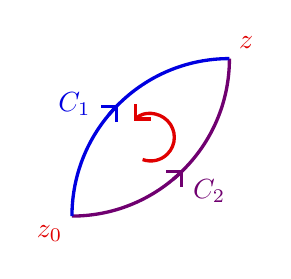
\begin{tikzpicture}
			\coordinate (O);
			\coordinate (A) at (2,2);
			\coordinate (C) at ({2+2*cos(145)},{2*sin(145)});
			\coordinate (D) at ({2*cos(-45)},{2+2*sin(-45)});
			\draw (O) node[below left,second] {$z_0$};
			\draw (A) node[above right,second] {$z$};
			\draw (C) node[above left,main] {$C_1$};
			\draw (D) node[below right,third] {$C_2$};
			\begin{scope}[cstcurve]
				\draw[third] (A) arc(0:-90:2);
				\draw[third,cstwra] ({2*cos(-50)},{2+2*sin(-50)}) arc(-50:-45:2);
				\draw[main] (O) arc(180:90:2);
				\draw[main,cstwra] ({2+2*cos(140)},{2*sin(140)}) arc(140:135:2);
				\draw[second,cstwla,visible on=<2->] ({1+0.3*cos(135)},{1+0.3*sin(135)}) arc(135:-110:0.3);
			\end{scope}
		\end{tikzpicture}
	\end{center}
\end{frame}


\begin{frame}{积分路径无关的函数特点}
	\onslide<+->
	上一节中我们计算了 $f(z)=z,\Re z,\dfrac1{z-z_0}$ 的积分.
	\onslide<+->
	其中
	\begin{itemize}
		\item $f(z)=z$ 处处解析, 积分只与起点终点有关 (闭路积分为零);
		\item $f(z)=\dfrac1{z-z_0}$ 有奇点 $z_0$, 沿绕 $z_0$ 闭路的积分非零;
		\item $f(z)=\Re z$ 处处不解析, 积分与路径有关 (闭路积分可能非零).
	\end{itemize}
	\onslide<+->
	由此可见函数沿闭路积分为零,
	\onslide<+->
	与函数在闭路内部是否解析有关.
\end{frame}


\begin{frame}{柯西-古萨基本定理: 推导}
	\onslide<+->
	设 $C$ 是一条闭路, $D$ 是其内部区域.
	\onslide<+->
	设 \emph{$f(z)$ 在闭区域 $\ov D=D\cup C$ 上解析},
	\onslide<+->
	即存在区域 $B\supseteq\ov D$ 使得 $f(z)$ 在 $B$ 上解析.

	\onslide<+->
	为了简便假设 $f'(z)$ 连续,
	\onslide<+->
	则
	\[\oint_Cf(z)\diff z=\oint_C(u\diff x-v\diff y)
	+i\oint_C(v\diff x+u\diff y).\]
	\onslide<+->
	由格林公式和C-R方程可知
	\[\oint_Cf(z)\diff z=-\iint_D(v_x+u_y)\diff x\diff y
	+i\iint_D(u_x-v_y)\diff x\diff y=0.\]
	\onslide<+->
	也可以从
	\[\oint_Cf(z)\diff z=-\iint_D\frac{\partial f}{\partial \ov z}\diff z\diff \ov z=2i\iint_D\frac{\partial f}{\partial \ov z}\diff x\diff y=0\]
	看出.
\end{frame}


\begin{frame}{柯西-古萨基本定理}
	\onslide<+->
	\begin{second}{柯西-古萨基本定理}
	设 $f(z)$ 在闭路 $C$ 上连续, $C$ 内部解析, 则 $\displaystyle\oint_Cf(z)\diff z=0$.
	\end{second}

	\onslide<+->
	\begin{corollary}
	设 $f(z)$ 在\alert{单连通域} $D$ 内解析, $C$ 是 $D$ 内一条闭合曲线, 则 $\displaystyle\oint_Cf(z)\diff z=0$.
	\end{corollary}
	\onslide<+->
	这里的闭合曲线可以不是闭路.

	% \onslide<+->
	% 这是因为即使不是简单曲线也可以拆分为一些简单曲线.
	% \onslide<4->
	% \begin{center}
	% 	\begin{tikzpicture}
	% 		\draw[cstcurve,main,smooth,domain=-45:-15] plot({3*sqrt(cos(2*\x))*cos(\x)},{3*sqrt(cos(2*\x))*sin(\x)});
	% 		\draw[cstcurve,main,smooth,domain=-20:45,cstwla] plot({3*sqrt(cos(2*\x))*cos(\x)},{3*sqrt(cos(2*\x))*sin(\x)});
	% 		\draw[cstcurve,main,smooth,domain=-45:-15] plot({-2*sqrt(cos(2*\x))*cos(\x)},{2*sqrt(cos(2*\x))*sin(\x)});
	% 		\draw[cstcurve,main,smooth,domain=-20:45,cstwla] plot({-2*sqrt(cos(2*\x))*cos(\x)},{2*sqrt(cos(2*\x))*sin(\x)});
	% 		\draw[cstcurve,second,cstwla,ultra thick] (1.05,0.35) arc (135:-135:0.5);
	% 		\draw[cstcurve,third,cstwla,ultra thick] (-0.75,-0.25) arc (315:45:0.3535);
	% 	\end{tikzpicture}
	% \end{center}
\end{frame}


\begin{frame}{典型例题: 柯西-古萨基本定理计算积分}
	\onslide<+->
	\begin{example}
		求 $\displaystyle\oint_{|z|=1}\frac1{2z-3}\diff z$.
	\end{example}

	\onslide<+->
	\begin{solution}
		由于 $\dfrac1{2z-3}$ 在 $|z|\le 1$ 上解析,
		\onslide<+->{因此由柯西-古萨基本定理 $\displaystyle \oint_{|z|=1}\frac1{2z-3}\diff z=0$.}
	\end{solution}

	\onslide<+->
	\begin{exercise}
		\begin{enumerate}
			\item $\displaystyle\oint_{|z-2|=1}\frac1{z^2+z}\diff z=$\fillblankframe{$0$}.
			\item 求 $\displaystyle\oint_{|z|=2}\dfrac{\sin z}{|z|}\diff z=$\fillblankframe{$0$}.
		\end{enumerate}
	\end{exercise}
\end{frame}


\begin{frame}{例: 柯西-古萨基本定理计算积分}
	\onslide<+->
	\begin{example}
		求 $\displaystyle\oint_C\frac1{z(z^2+1)}\diff z$, 其中 $C:|z-i|=\dfrac12$.
	\end{example}

	\onslide<+->
	\begin{solution}
		注意到 $\dfrac1{z(z^2+1)}=\dfrac1z-\dfrac12\left(\dfrac1{z+i}+\dfrac1{z-i}\right)$.
		\onslide<+->{由于 $\dfrac1z,\dfrac1{z+i}$ 在 $|z-i|\le\dfrac12$ 上解析,
		}\onslide<+->{因此由柯西-古萨基本定理
			\[\oint_C\frac1z\diff z
			=\oint_C\frac1{z+i}\diff z=0,\]
		}\onslide<+->{
			\[\oint_C\frac1{z(z^2+1)}\diff z
			=-\half\oint_C\frac1{z-i}\diff z=-\pi i.\]}
	\end{solution}
\end{frame}


\subsection{复合闭路定理}

\begin{frame}{多连通域边界与复合闭路}
	\onslide<+->
	设 $C_0,C_1,\dots,C_n$ 是 $n+1$ 条简单闭曲线, $C_1,\dots,C_n$ 每一条都包含在其它闭路的外部, 而且它们都包含在 $C_0$ 的内部.
	\onslide<+->
	这样它们围成了一个多连通区域 $D$, 它的边界称为一个\emph{复合闭路} \[C=C_0+C_1^-+\cdots+C_n^-.\]
	\onslide<+->
	沿着 $C$ 前进的点, $D$ 总在它的左侧,所以这就是它的正方向.
	\onslide<1->
	\begin{center}
		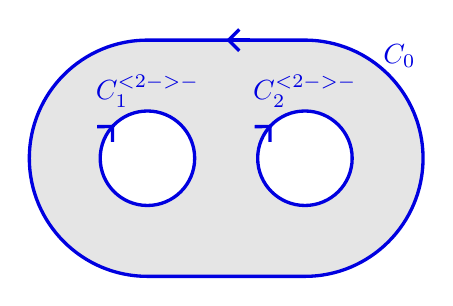
\begin{tikzpicture}
			\fill[cstfill,visible on=<2->,rounded corners=15mm] (-2.5,-1.5) rectangle (2.5,1.5);
			\draw[cstcurve,main,rounded corners=15mm] (-2.5,-1.5) rectangle (2.5,1.5);
			\fill[cstcurve,white,visible on=<2->] (1,0) circle(0.6);
			\fill[cstcurve,white,visible on=<2->] (-1,0) circle(0.6);
			\draw[cstcurve,main] (1,0) circle(0.6);
			\draw[cstcurve,main] (-1,0) circle(0.6);
			\draw[cstcurve,main,domain=85:90,cstwra,visible on=<2->] plot (.3,1.5)--(0,1.5);
			\draw[cstcurve,main,domain=135:140,cstwla,visible on=<2->] plot ({1+0.6*cos(\x)}, {0.6*sin(\x)});
			\draw[cstcurve,main,domain=135:140,cstwla,visible on=<2->] plot ({-1+0.6*cos(\x)}, {0.6*sin(\x)});
			\draw
				(2.2,1.3) node[main] {$C_0$}
				(-1,0.85) node[main] {$C_1^{\visible<2->-}$}
				(1,0.85) node[main] {$C_2^{\visible<2->-}$};
		\end{tikzpicture}
	\end{center}
\end{frame}


\begin{frame}{复合闭路定理}
	\onslide<+->
	\begin{second}{复合闭路定理}
		设 $f(z)$ 在复合闭路 $C=C_0+C_1^-+\cdots+C_n^-$ 及其所围成的多连通区域内解析, 则
		\[\oint_{C_0}f(z)\diff z=
		\oint_{C_1}f(z)\diff z+\cdots+\oint_{C_n}f(z)\diff z.\]
	\end{second}
	\onslide<+->
	事实上, 复合闭路定理和柯西-古萨基本定理可以看成一个定理的两种情形: 
	\onslide<+->
	设 $C$ 是一个闭路或复合闭路, 若 $f(z)$ 在 $C$ 及其围成的区域(单连通或多连通)内解析, 则 $\displaystyle\oint_Cf(z)\diff z=0$.
\end{frame}



\begin{frame}{复合闭路定理: 注记}
	\onslide<+->
	在实际应用中, 如果被积函数 $f(z)$ 在(复合)闭路 $C$ 的内部有有限多个奇点 $z_1,\dots,z_k$.
	\onslide<+->
	那么我们可以在 $C$ 内部(围成的区域)构造闭路 $C_1,\dots,C_k$, 使得每个 $C_j$ 内部只包含一个奇点 $z_j$.
	\onslide<+->
	这样, 内部含多个奇点的情形就可以化成内部只含一个奇点的情形. 最后将这些闭路上的积分相加即可.
	\onslide<1->
	\begin{center}
		\begin{tikzpicture}
			\draw[cstcurve,main,rounded corners=10mm] (-2.2,-1.2) rectangle (2.2,1.2);
			\draw[cstcurve,second,visible on=<2->] (1,0) circle(0.4);
			\draw[cstcurve,second,visible on=<2->] (0,0) circle(0.4);
			\draw[cstcurve,second,visible on=<2->] (-1,0) circle(0.4);
			\fill[cstdot,second] (1,0) circle;
			\fill[cstdot,second] (0,0) circle;
			\fill[cstdot,second] (-1,0) circle;
			\draw
				(-1,-0.25) node[second] {$z_1$}
				(0,-0.25) node[second] {$z_2$}
				(1,-0.25) node[second] {$z_3$}
				(2.2,1.1) node[main] {$C$}
				(-1,0.65) node[second,visible on=<2->] {$C_1$}
				(0,0.65) node[second,visible on=<2->] {$C_2$}
				(1,0.65) node[second,visible on=<2->] {$C_3$};
		\end{tikzpicture}
	\end{center}
\end{frame}


\begin{frame}{复合闭路定理: 注记}
	\onslide<+->
	此外, 从复合闭路定理还可以看出, 在计算积分 $\displaystyle \oint_C f(z)\diff z$ 时, $C$ 的具体形状无关紧要, 只要其内部奇点不变, $C$ 可以任意变形.
	\onslide<+->
	因为我们总可以选择一个包含这些奇点的闭路 $C'$, 使得 $C'$ 包含在 $C$ 及其变形后的闭路内部. 这样它们的积分自然都和 $C'$ 上的积分相同.
	\onslide<+->
	这里即使 $C$ 是复合闭路也是可以自由变形的.
	\onslide<1->
	\begin{center}
		\begin{tikzpicture}
			\draw[cstcurve,main,rounded corners=10mm] (-2.2,-1.2) rectangle (2.2,1.2);
			\draw[cstcurve,third] (0,0) circle(1.2 and 2.2);
			\draw[cstcurve,second,visible on=<2->] (0,0) circle(1);
			\fill[cstdot,second] (.7,0.2) circle;
			\fill[cstdot,second] (0,-0.4) circle;
			\fill[cstdot,second] (-.5,0.1) circle;
			\draw
				(2,1.4) node[main] {$C_1$}
				(-1.1,1.8) node[third] {$C_2$}
				(-.4,0.65) node[second,visible on=<2->] {$C'$};
		\end{tikzpicture}
	\end{center}
\end{frame}


\begin{frame}{复合闭路定理}
	\onslide<+->
	\begin{proof}
		以曲线 $\gamma_1,\gamma_2,\dots,\gamma_{n+1}$ 把 $C_0,C_1,\dots,C_n$ 连接起来, 则它们把区域 $D$ 分成了两个单连通域 $D_1,D_2$.
		\onslide<+->{对 $D_1$ 和 $D_2$ 的边界应用柯西-古萨基本定理并相加, 则 $\gamma_i$ 对应的部分正好相互抵消,
		}\onslide<+->{因此
			\[\oint_{C_0}f(z)\diff z-
		\oint_{C_1}f(z)\diff z-\cdots-\oint_{C_n}f(z)\diff z=0.\]
		}\onslide<+->{于是定理得证.\qedhere}
		\vspace{-1.7\baselineskip}
		\onslide<1->
		\begin{center}
			\begin{tikzpicture}[scale=.9]
				\fill[cstcurve,cstfill] (0,0) circle(2.5 and 1.5);
				\fill[cstcurve,white] (1,0) circle(0.6);
				\fill[cstcurve,white] (-1,0) circle(0.6);

				\draw[cstcurve,main,domain=0:90,cstwra] plot ({2.5*cos(\x)}, {1.5*sin(\x)});
				\draw[cstcurve,main,domain=85:180] plot ({2.5*cos(\x)}, {1.5*sin(\x)});
				\draw[cstcurve,second,domain=180:270,cstwra] plot ({2.5*cos(\x)}, {1.5*sin(\x)});
				\draw[cstcurve,second,domain=265:360] plot ({2.5*cos(\x)}, {1.5*sin(\x)});

				\draw[cstcurve,main,domain=0:140] plot ({1+0.6*cos(\x)}, {0.6*sin(\x)});
				\draw[cstcurve,main,domain=135:180,cstwla] plot ({1+0.6*cos(\x)}, {0.6*sin(\x)});
				\draw[cstcurve,second,domain=180:320] plot ({1+0.6*cos(\x)}, {0.6*sin(\x)});
				\draw[cstcurve,second,domain=315:360,cstwla] plot ({1+0.6*cos(\x)}, {0.6*sin(\x)});

				\draw[cstcurve,main,domain=0:140] plot ({-1+0.6*cos(\x)}, {0.6*sin(\x)});
				\draw[cstcurve,main,domain=135:180,cstwla] plot ({-1+0.6*cos(\x)}, {0.6*sin(\x)});
				\draw[cstcurve,second,domain=180:320] plot ({-1+0.6*cos(\x)}, {0.6*sin(\x)});
				\draw[cstcurve,second,domain=315:360,cstwla] plot ({-1+0.6*cos(\x)}, {0.6*sin(\x)});

				\draw
					(2,1.3) node[main] {$C_0$}
					(-1,0.85) node[main] {$C_1^-$}
					(1,0.85) node[main] {$C_2^-$}
					(-2,-0.3) node {$\gamma_1$}
					(0,-0.3) node {$\gamma_2$}
					(2,-0.3) node {$\gamma_3$};
				\draw[cstcurve] (-2.5,0)--(-1.6,0);
				\draw[cstcurve] (-0.4,0)--(0.4,0);
				\draw[cstcurve] (1.6,0)--(2.5,0);
				\draw[cstcurve,thick,main,visible on=<2->] (-2.5,0.025)--(-1.6,0.025);
				\draw[cstcurve,thick,second,visible on=<2->] (-2.5,-0.025)--(-1.6,-0.025);
				\draw[cstcurve,thick,main,visible on=<2->] (-0.4,0.025)--(0.4,0.025);
				\draw[cstcurve,thick,second,visible on=<2->] (-0.4,-0.025)--(0.4,-0.025);
				\draw[cstcurve,thick,main,visible on=<2->] (1.6,0.025)--(2.5,0.025);
				\draw[cstcurve,thick,second,visible on=<2->] (1.6,-0.025)--(2.5,-0.025);
			\end{tikzpicture}
		\end{center}
		\vspace{-\baselineskip}
	\end{proof}
\end{frame}


\begin{frame}{例: 复合闭路定理的应用}
	\onslide<+->
	\begin{example}
		证明对于任意闭路 $C$, $\displaystyle\int_C(z-a)^n\diff z=0$, $n\neq -1$ 为整数.
	\end{example}

	\onslide<+->
	\begin{proof}
		\begin{enumerate}
			\item 如果 $a$ 不在 $C$ 的内部, 则 $(z-a)^n$ 在 $C$ 及其内部解析.
			\onslide<+->{%
				由柯西-古萨基本定理, $\displaystyle\int_C(z-a)^n\diff z=0$.
			}
			\item 如果 $a$ 在 $C$ 的内部, 则在 $C$ 的内部取一个以 $a$ 为圆心的圆周 $C_1$.
			\onslide<+->{%
				由复合闭路定理以及上一节的结论
				\[
					\int_C(z-a)^n\diff z=\int_{C_1}(z-a)^n\diff z=0.\qedhere
				\]
			}
			\vspace{-\baselineskip}
		\end{enumerate}
	\end{proof}
\end{frame}


\begin{frame}{例: 复合闭路定理的应用}
	\onslide<+->
	同理, 由复合闭路定理和上一节的结论可知当 $a$ 在 $C$ 的内部且 $n=-1$ 时积分为 $2\pi i$.
	\onslide<+->
	\begin{theorem@}
		当 $a$ 在 $C$ 的内部时,
		\[\oint_C\frac{\diff z}{(z-a)^{n+1}}=\begin{cases}2\pi i,&n=0;\\0,&n\neq 0.\end{cases}\]
	\end{theorem@}
\end{frame}


\begin{frame}{例: 复合闭路定理的应用}
	\beqskip{4pt}
	\onslide<+->
	\begin{example}
		\begin{minipage}{.6\textwidth}
			求 $\displaystyle\int_\Gamma\frac{2z-1}{z^2-z}\diff z$, 其中 $\Gamma$ 是由 $2\pm i,-2\pm i$ 形成的矩形闭路.
		\end{minipage}
		\begin{minipage}{.36\textwidth}
			\begin{tikzpicture}
				\draw[cstaxis] (-2.5,0)--(2.5,0);
				\draw[cstaxis] (0,-1)--(0,1);
				\draw[cstcurve,cstwra,main] (-1,-0.7)--(-0.5,-0.7);
				\draw[cstcurve,cstwra,second,visible on=<3->] (-0.4,0) arc(180:225:0.4);
				\draw[cstcurve,cstwra,second,visible on=<3->] (0.6,0) arc(180:225:0.4);
				\draw[cstcurve,second,visible on=<3->] (0,0) circle (0.4);
				\draw[cstcurve,second,visible on=<3->] (1,0) circle (0.4);
				\fill[cstdot,third,visible on=<2->] (1,0) circle;
				\fill[cstdot,third,visible on=<2->] (0,0) circle;
				\draw[cstcurve,main] (-2,-0.7) rectangle (2,0.7);
				\draw
					(-0.6,0.4) node[second,visible on=<3->] {$C_1$}
					(1.6,0.4) node[second,visible on=<3->] {$C_2$}
					(-1,-0.5) node[main] {$\Gamma$};
			\end{tikzpicture}
		\end{minipage}
	\end{example}
	\onslide<+->
	\begin{solution}
		函数 $\dfrac{2z-1}{z^2-z}$ 在 $\Gamma$ 内有两个奇点 $z=0,1$.
		\onslide<+->{%
			设 $C_1,C_2$ 如图所示,
		}\onslide<+->{%
			由复合闭路定理
			\begin{align*}
				&\oint_\Gamma\frac{2z-1}{z^2-z}\diff z
				=\oint_{C_1}\frac{2z-1}{z^2-z}\diff z+\oint_{C_2}\frac{2z-1}{z^2-z}\diff z\\
				\visible<+->{=}&\visible<.->{\oint_{C_1}\frac1z\diff z+\oint_{C_1}\frac1{z-1}\diff z
				+\oint_{C_2}\frac1z\diff z+\oint_{C_2}\frac1{z-1}\diff z}\\
				\visible<+->{=}&\visible<.->{2\pi i+0+0+2\pi i=4\pi i.}
			\end{align*}
		}\vspace{-\baselineskip}
	\end{solution}
	\endgroup
\end{frame}


\begin{frame}{例: 复合闭路定理的应用}
	\onslide<+->
	\begin{example}
		求 $\displaystyle\int_\Gamma\frac{e^z}z\diff z$, 其中 $\Gamma=C_1+C_2^-$, $C_1:|z|=2, C_2:|z|=1$.
		\vspace{-.8\baselineskip}
		\begin{center}
			\begin{tikzpicture}[scale=.8]
				\filldraw[cstcurve,main,cstfill] (0,0) circle (1.5);
				\draw[cstcurve,main,cstwla] (-1.06,1.06) arc(135:90:1.5);
				\filldraw[cstcurve,second,fill=white] (0,0) circle (0.75);
				\draw[cstcurve,second,cstwra] (-0.75,0) arc(180:130:0.75);
				\draw
					(-1.6,0.8) node[main] {$C_1$}
					(0.8,-0.7) node[second] {$C_2^-$};
				\draw[cstaxis] (-1.8,0)--(1.8,0);
				\draw[cstaxis] (0,-1.8)--(0,1.8);
			\end{tikzpicture}
		\end{center}
		\vspace{-.8\baselineskip}
	\end{example}
	\onslide<+->
	\begin{solution}
		函数 $\dfrac{e^z}z$ 在 $C_1,C_2$ 围城的圆环域内解析.
		\onslide<+->{由复合闭路定理可知 $\displaystyle\int_\Gamma\frac{e^z}z\diff z=0$.}
	\end{solution}
\end{frame}



\section{原函数和不定积分}

\subsection{原函数}

\begin{frame}{原函数的存在性}
	\onslide<+->
	设 $f(z)$ 在单连通域 $D$ 内解析, $C$ 是 $D$ 内一条起于 $z_0$ 终于 $z$ 的曲线.
	\onslide<+->
	由柯西-古萨基本定理可知, 积分 $\displaystyle\int_Cf(\zeta)\diff \zeta$ 与路径无关, 只与 $z_0,z$ 有关.
	\onslide<+->
	因此我们也将其记为 $\displaystyle\int_{z_0}^zf(\zeta)\diff\zeta$.

	\onslide<+->
	对于任意固定的 $z_0\in D$, 定义
	\[F(z)=\int_{z_0}^zf(\zeta)\diff\zeta.\]
\end{frame}


\begin{frame}{原函数的存在性}
	\beqskip{0pt}
	\onslide<+->
	\begin{theorem}
		$F(z)$ 是 $D$ 内的解析函数, 且 $F'(z)=f(z)$.
	\end{theorem}
	\onslide<+->
	\begin{solution}[证明]
		\begin{center}
			\begin{tikzpicture}
				\fill[cstcurve,main,rounded corners=0.5cm,cstfill] (-2.5,-0.8) rectangle (2,1);
				\draw[cstcurve,main] (0,0) circle(0.7);
				\draw[cstcurve,third] (-2,0)to [bend left](0,0);
				\draw[cstcurve,third,visible on=<2->] (0,0)--(0.4,0.4);
				\fill[cstdot,third] (-2,0) circle;
				\fill[cstdot,third] (0,0) circle;
				\fill[cstdot,third,visible on=<2->] (0.4,0.4) circle;
				\draw
					(-2,-0.3) node[third] {$z_0$}
					(0,-0.3) node[third] {$z$}
					(1.1,0.7) node[third,visible on=<2->] {$z+\Delta z$};
			\end{tikzpicture}
		\end{center}
		以 $z$ 为中心作一包含在 $D$ 内的圆 $K$,
		\onslide<+->{%
			取 $|\Delta z|$ 小于 $K$ 的半径.
		}\onslide<+->{%
			那么
			\[
				F(z+\Delta z)-F(z)=\int_{z_0}^{z+\Delta z}f(\zeta)\diff\zeta-\int_{z_0}^zf(\zeta)\diff\zeta
				\visible<+->{=\int_z^{z+\Delta z}f(\zeta)\diff\zeta.}
			\]
		}\onslide<+->{%
			容易知道
			$\displaystyle\int_z^{z+\Delta z}f(z)\diff\zeta=f(z)\int_z^{z+\Delta z}\diff\zeta=f(z)\Delta z$.
		}\onslide<+->{%
			我们需要比较上述两个积分, 其中 $z$ 到 $z+\Delta z$ 取直线.
		}
	\end{solution}
	\endgroup
\end{frame}


\begin{frame}{原函数的存在性}
	\onslide<+->
	\begin{proof}[续证]
		由于 $f(z)$ 解析, 因此连续.
		\onslide<+->{$\forall\varepsilon>0,\exists\delta>0$ 使得当 $|\zeta-z|<\delta$ 时, $z$ 落在 $K$ 中且 $|f(\zeta)-f(z)|<\varepsilon$.
		}\onslide<+->{当 $|\Delta z|<\delta$ 时, 由长大不等式
			\begin{align*}
			\abs{\frac{F(z+\Delta z)-F(z)}{\Delta z}-f(z)}
			&\visible<+->{=\abs{\int_z^{z+\Delta z}\frac{f(\zeta)-f(z)}{\Delta z}\diff \zeta}}\\
			&\visible<+->{\le\frac{\varepsilon}{|\Delta z|}\cdot|\Delta z|=\varepsilon.}
			\end{align*}
		}\onslide<+->{由于 $\varepsilon$ 是任意的, 因此
		\[f(z)=\lim_{\Delta z\to 0}\frac{F(z+\Delta z)-F(z)}{\Delta z}=F'(z).\qedhere\]}
	\end{proof}
\end{frame}


\subsection{牛顿-莱布尼兹定理}

\begin{frame}{牛顿-莱布尼兹定理}

	\onslide<+->
	如果 $D$ 上的解析函数 $G(z)$ 满足 $G'(z)=f(z)$, 则称 $G(z)$ 是 $f(z)$ 的一个\emph{原函数}.
	\onslide<+->
	由于导函数为 $0$ 的解析函数只能是常值函数,
	\onslide<+->
	因此 $\displaystyle G(z)=\int_{z_0}^zf(\zeta)\diff \zeta+C$.
	\onslide<+->
	我们称之为 $f(z)$ 的\emph{不定积分}, 记为 \emph{$\displaystyle\int f(z)\diff z$}.

	\onslide<+->
	\begin{second}{复变函数积分计算方法II}
		设 $f(z)$ 在单连通区域 $D$ 上解析, $z_1$ 至 $z_2$ 的积分路径落在 $D$ 内, 则
		\[
			\int_{z_1}^{z_2}f(z)\diff z=F(z)\Big|_{z_1}^{z_2}=F(z_2)-F(z_1),\]
		其中 $F(z)$ 是 $f(z)$ 的一个原函数.
	\end{second}

	\onslide<+->
	复变函数和实变函数的牛顿-莱布尼兹定理的差异在哪呢?
	\onslide<+->
	复变情形要求是\alert{单连通区域上解析函数}, 实变情形要求是\alert{闭区间上连续函数}.
\end{frame}


\begin{frame}{典型例题: 利用原函数求积分}
	\onslide<+->
	\begin{example}
		求 $\displaystyle\int_{z_0}^{z_1}z\diff z$.
	\end{example}

	\onslide<+->
	\begin{solution}
		由于 $f(z)=z$ 处处解析,
		\onslide<+->{%
			且 $\displaystyle\int z\diff z=\half  z^2+C$,
		}\onslide<+->{%
			因此
			\[
				\int_{z_0}^{z_1}z\diff z=\half z^2\big|_{z_0}^{z_1}=\half (z_1^2-z_0^2).
			\]
		}\vspace{-.5\baselineskip}
	\end{solution}
	\onslide<+->
	因此之前的例子中 $\displaystyle\int_0^{3+4i}z\diff z=-\frac72+12i$, 无论从 $0$ 到 $3+4i$ 的路径如何.
\end{frame}


\begin{frame}{典型例题: 利用原函数求积分}
	\onslide<+->
	\begin{example}
		求 $\displaystyle\int_0^{\pi i}z\cos z^2\diff z$.
	\end{example}

	\onslide<+->
	\begin{solution}
		由于 $f(z)=z\cos z^2$ 处处解析,
		\onslide<+->{%
			且
			\[
				\int z\cos z^2\diff z=\half\int \cos z^2\diff z^2=\half\sin z^2+C,
			\]
		}\onslide<+->{%
			因此
			\[
				\int_0^{\pi i}z\cos z^2\diff z=\half\sin z^2\big|_0^{\pi i}=-\half\sin \pi^2.
			\]
		}\vspace{-.5\baselineskip}
	\end{solution}

	\onslide<+->
	这里我们使用了\alert{凑微分法}.
\end{frame}


\begin{frame}{典型例题: 利用原函数求积分}
	\onslide<+->
	\begin{example}
		求 $\displaystyle\int_0^i z\cos z\diff z$.
	\end{example}

	\onslide<+->
	\begin{solution}
		由于 $f(z)=z\cos z$ 处处解析,
		\onslide<+->{%
			且
			\[
				\int z\cos z\diff z
				=\int z\diff(\sin z)
				=z\sin z-\int \sin z\diff z
				\visible<+->{=z\sin z+\cos z+C,}
			\]
		}\onslide<+->{%
			因此
			\[
				\int_0^i z\cos z\diff z
				=(z\sin z+\cos z)\big|_0^i
				\visible<+->{=i\sin i+\cos i-1=e^{-1}-1.}
			\]
		}\vspace{-.5\baselineskip}
	\end{solution}
	\onslide<+->
	这里我们使用了\alert{分部积分法}.
\end{frame}


\begin{frame}{典型例题: 利用原函数求积分}
	\onslide<+->
	\begin{example}
		求 $\displaystyle\int_1^{1+i} z e^z\diff z$.
	\end{example}
	\onslide<+->
	\begin{solution}
		由于 $f(z)=ze^z$ 处处解析,
		\onslide<+->{%
			且 $\displaystyle\int z e^z\diff z=\int z\diff e^z=ze^z-\int e^z\diff z=(z-1)e^z+C$,
		}\onslide<+->{%
			因此 $\displaystyle \int_1^{1+i} z e^z\diff z=(z-1)e^z\big|_1^{1+i}
			\visible<+->{=ie^{1+i}=e(-\sin 1+i\cos 1)}$.
		}
	\end{solution}
	\onslide<+->
	\begin{exercise}
		求 $\displaystyle\int_0^1 z\sin z\diff z=$\fillblankframe[4cm]{$\sin 1-\cos 1$}.
	\end{exercise}
\end{frame}


\begin{frame}{典型例题: 利用原函数求积分}
	\beqskip{0pt}
	\onslide<+->
	\begin{example}
		求 $\displaystyle\int_C(2z^2+8z+1)\diff z$, 其中 $C$ 是摆线
		$\displaystyle\begin{cases}
		x=a(\theta-\sin\theta),& \\ y=a(1-\cos\theta),
		\end{cases} 0\le \theta\le 2\pi.$
		\vspace{-\baselineskip}
		\begin{center}
			\begin{animateinline}[width=9cm]{10}
				\begin{tikzpicture}
					\draw[cstaxis, thick](-1.5,0)--(7.5,0);
					\draw[cstaxis, thick](0,0)--(0,2.5);
					\draw[cstcurve,main,smooth,domain=0:360] plot ({1*(pi/180*\x-sin(\x))},{1*(1-cos(\x))});
				\end{tikzpicture}
				\newframe
				\multiframe{37}{r=0+10}{
					\begin{tikzpicture}
						\draw[cstaxis, thick](-1.5,0)--(7.5,0);
						\draw[cstaxis, thick](0,0)--(0,2.5);
						\draw[cstcurve,second] ({1*(pi/180*\r)},1) circle (1);
						\fill[cstdot,main] ({1*(pi/180*\r-sin(\r))},{1*(1-cos(\r))}) circle;
						\draw[cstcurve,main,smooth,domain=0:360] plot ({1*(pi/180*\x-sin(\x))},{1*(1-cos(\x))});
					\end{tikzpicture}
				}
			\end{animateinline}
		\end{center}
	\end{example}
	\onslide<+->
	\begin{solution}
		由于 $f(z)=2z^2+8z+1$ 处处解析,
		\onslide<+->{%
			因此
			\[
				\text{原积分}=\int_0^{2\pi a}(2z^2+8z+1)\diff z
				\visible<+->{=\left(\frac23z^3+4z^2+z\right)\bigg|_0^{2\pi a}=\frac{16}3\pi^3a^3+16\pi^2a^2+2\pi a.}
			\]
		}
	\end{solution}
	\endgroup
\end{frame}


\begin{frame}{典型例题: 利用原函数求积分}
	\beqskip{3pt}
	\onslide<+->
	\begin{example}
		设 $C$ 为沿着 $|z|=1$ 从 $1$ 到 $i$ 的逆时针圆弧, 求 $\displaystyle\int_C\frac{\ln(z+1)}{z+1}\diff z$.
	\end{example}

	\onslide<+->
	\begin{solution}
		函数 $f(z)=\dfrac{\ln(z+1)}{z+1}$ 在单连通区域 $\Re z>-1$ 内解析.
		\onslide<+->{%
			\[\int\frac{\ln(z+1)}{z+1}\diff z
			=\int\ln(z+1)\diff[\ln(z+1)]=\half\ln^2(z+1)+C.\]
		}\onslide<+->{%
			因此
			\begin{align*}
				\int_C\frac{\ln(z+1)}{z+1}\diff z&=\half\ln^2(z+1)\big|_1^i
				\visible<+->{=\half\left[\ln^2(1+i)-\ln^22\right]}\\
				&\visible<+->{=\half\biggl(\Bigl(\ln\sqrt2+\frac\pi4i\Bigr)^2-\ln^22\biggr)
				=-\frac{\pi^2}{32}-\frac38\ln^22+\frac{\pi\ln2}{8}i.}
			\end{align*}
		}
	\end{solution}
	\endgroup
\end{frame}



\section{柯西积分公式}


\begin{frame}{柯西积分公式}
\onslide<+->
柯西积分定理是解析函数理论的基础, 但在很多情形下它由柯西积分公式表现.
\begin{block}{柯西积分公式}
设
\begin{itemize}[<*>]
\item 函数 $f(z)$ 在闭路或复合闭路 $C$ 及其内部 $D$ 解析,
\item $z_0\in D$,
\end{itemize}
\onslide<+->
则
\[f(z_0)=\frac1{2\pi i}\oint_C\frac{f(z)}{z-z_0}\diff z.\]
\end{block}
\onslide<+->
如果 $z_0\notin D$, 由柯西-古萨基本定理, 右侧的积分是 $0$.
\end{frame}


\begin{frame}{柯西积分公式: 注记}
\begin{enumerate}
\item 解析函数可以用一个积分
\[f(z)=\frac1{2\pi i}\oint_C\frac{f(\zeta)}{\zeta-z}\diff\zeta,\quad z\in D\]
来表示, 这是研究解析函数理论的强有力工具.
\item 求积分 $\displaystyle\oint_C g(z)\diff z$ 时, 如果 $g(z)$ 在 $C$ 内部只有一个奇点 $z_0$, 且 $g(z)(z-z_0)$ 解析, 那么我们就可以使用柯西积分公式来计算该积分.
\item 解析函数在闭路 $C$ 内部的取值完全由它在 $C$ 上的值所确定. 这也是解析函数的特征之一.

\onslide<+->
\indent
特别地, 解析函数在圆心处的值等于它在圆周上的平均值.
\onslide<+->
设 $z=z_0+Re^{i\theta}$, 则 $\diff z=iRe^{i\theta}\diff\theta$,
\onslide<+->
\[f(z_0)=\frac1{2\pi i}\oint_C\frac{f(z)}{z-z_0}\diff z=\frac1{2\pi}\int_0^{2\pi}f(z_0+Re^{i\theta})\diff\theta.\]
\end{enumerate}
\end{frame}


\begin{frame}{柯西积分公式: 证明}
\begin{proof}
由连续性可知, $\forall\varepsilon>0,\exists\delta>0$ 使得当 $|z-z_0|<\delta$ 时, $z\in D$ 且 $|f(z)-f(z_0)|<\varepsilon$.
\onslide<+->
设 $\Gamma:|z-z_0|=r<\delta$.
\onslide<+->
由复合闭路定理和长大不等式
\begin{align*}
&\peq\abs{\oint_C\frac{f(z)}{z-z_0}\diff z-2\pi i f(z_0)}
=\abs{\oint_\Gamma\frac{f(z)}{z-z_0}\diff z-2\pi i f(z_0)}\\
&\visible<+->{=\abs{\oint_\Gamma\frac{f(z)}{z-z_0}\diff z-\oint_\Gamma\frac{f(z_0)}{z-z_0}\diff z}
=\abs{\oint_\Gamma\frac{f(z)-f(z_0)}{z-z_0}\diff z}}\\
&\visible<+->{\le \frac\varepsilon r\cdot 2\pi r=2\pi \varepsilon.}
\end{align*}
\onslide<+->
由 $\varepsilon$ 的任意性可知 $\displaystyle\oint_C\frac{f(z)}{z-z_0}\diff z=2\pi i f(z_0)$.
\end{proof}
\end{frame}


\begin{frame}{典型例题: 柯西积分公式的应用}
\begin{example}
求 $\displaystyle\oint_{|z|=4}\frac{\sin z}z\diff z$.
\end{example}
\begin{solution}
由于函数 $\sin z$ 处处解析,
\onslide<+->
因此由柯西积分公式
\[\oint_{|z|=4}\frac{\sin z}z\diff z
=2\pi i \sin z|_{z=0}=0.\]
\end{solution}
\end{frame}


\begin{frame}[<*>]{例题: 柯西积分公式的应用}
\onslide<+->
\begin{example}
求 $\displaystyle\oint_{|z|=2}\frac{e^z}{z-1}\diff z$.
\end{example}

\onslide<+->
\begin{solution}
由于函数 $e^z$ 处处解析,
\onslide<+->
因此由柯西积分公式
\[\oint_{|z|=2}\frac{e^z}{z-1}\diff z
=2\pi i e^z|_{z=1}=2\pi ei.\]
\end{solution}

\onslide<+->
\begin{columns}
	\column{0.48\textwidth}
		\begin{exercise}
		求 $\displaystyle\oint_{|z|=2\pi}\frac{\cos z}{z-\pi}\diff z$.
		\end{exercise}\onslide<+->
	\column{0.48\textwidth}
		\begin{answer}
		$-2\pi i\vphantom{\displaystyle\oint_{|z|=2\pi}\frac{\cos z}{z-\pi}\diff z}$.
		\end{answer}
\end{columns}
\end{frame}


\begin{frame}{例题: 柯西积分公式的应用}
\beqskip{5pt}
\begin{example}
设 $f(z)=\displaystyle\oint_{|\zeta|=\sqrt3}\frac{3\zeta^2+7\zeta+1}{\zeta-z}\diff \zeta$, 求 $f'(1+i)$.
\end{example}
\begin{solution}
由柯西积分公式, 当 $|z|<\sqrt3$ 时,
\begin{align*}
f(z)&=\oint_{|\zeta|=\sqrt3}\frac{3\zeta^2+7\zeta+1}{\zeta-z}\diff \zeta\\
&\visible<+->{=2\pi i(3\zeta^2+7\zeta+1)|_{\zeta=z}=2\pi i(3z^2+7z+1).}
\end{align*}
\onslide<+->
因此
\vspace{-\baselineskip}
\[f'(z)=2\pi i(6z+7),\]
\vspace{-\baselineskip}
\onslide<+->
\[f'(1+i)=2\pi i(13+6i)=-12\pi+26\pi i.\]
\end{solution}
\onslide<+->
注意当 $|z|>\sqrt3$ 时, $f(z)\equiv0$.
\endgroup
\end{frame}


\begin{frame}{例题: 柯西积分公式的应用}
\begin{example}
求 $\displaystyle\oint_{|z|=3}\frac{e^z}{z(z^2-1)}\diff z$.
\end{example}
\begin{solution}
被积函数的奇点为 $0,\pm1$.
\onslide<+->
设 $C_1,C_2,C_3$ 分别为绕 $0,1,-1$ 的分离圆周.
\onslide<1->
\begin{center}
\begin{tikzpicture}
\draw[cstaxis] (-1.3,0)--(1.3,0);
\draw[cstaxis] (0,-1.1)--(0,1.25);
\draw[cstcurve,dcolorb] (0,0) circle (1);
\draw[cstcurve,dcolora,visible on=<3->] (0.5,0) circle(0.2);
\draw[cstcurve,dcolora,visible on=<3->] (-0.5,0) circle(0.2);
\draw[cstcurve,dcolora,visible on=<3->] (0,0) circle(0.2);
\fill[cstdot,dcolorb,visible on=<2->] (0,0) circle;
\fill[cstdot,dcolorb,visible on=<2->] (0.5,0) circle;
\fill[cstdot,dcolorb,visible on=<2->] (-0.5,0) circle;
\draw
  (1,0.8) node[dcolorb] {$C$}
  (-0.3,0.45) node[dcolora,visible on=<3->] {$C_1$}
  (0.5,-0.45) node[dcolora,visible on=<3->] {$C_2$}
  (-0.5,-0.45) node[dcolora,visible on=<3->] {$C_3$};
\end{tikzpicture}
\end{center}
\end{solution}
\end{frame}


\begin{frame}{例题: 柯西积分公式的应用}
\begin{solutionc}
由复合闭路定理和柯西积分公式
\begin{align*}
&\peq\oint_{|z|=3}\frac{e^z}{z(z^2-1)}\diff z
=\oint_{C_1+C_2+C_3}\frac{e^z}{z(z^2-1)}\diff z\\
&\visible<+->{=2\pi i\left[\frac{e^z}{z^2-1}\bigg|_{z=0}+\frac{e^z}{z(z+1)}\bigg|_{z=1}+\frac{e^z}{z(z-1)}\bigg|_{z=-1}\right]}\\
&\visible<+->{=2\pi i\left(-1+\frac e2+\frac{e^{-1}}2\right)=\pi i(e+e^{-1}-2).}
\end{align*}
\end{solutionc}
\end{frame}


\begin{frame}[<*>]{典型例题: 计算复变函数沿曲线的积分}
\onslide<+->
\begin{columns}
	\column{0.48\textwidth}
		\begin{thinking}
		对于闭路 $C$ 的外部, 是否有类似的柯西积分公式?
		\end{thinking}
		\onslide<+->
	\column{0.48\textwidth}
		\begin{tikzpicture}
		\fill[cstfille] (2.8,1.6) rectangle (-2.8,-1.6);
		\filldraw[cstcurve,dcolora,rounded corners=0.3cm,fill=white] (-0.6,0.6) rectangle (-1.3,-0.6);
		\draw[cstcurve,visible on=<4->,dcolorc] (0,0) circle (0.4);
		\draw[cstcurve,visible on=<4->,dcolorb] (0,0) circle (1.5);
		\fill[cstdot,dcolora] (0,0) circle;
		\draw
		  (0,0.2) node[dcolora] {$z_0$}
		  (-0.6,-0.8) node[dcolora] {$C$}
		  (0.7,-0.2) node[dcolorc,visible on=<4->] {$C_1$}
		  (0.9,0.8) node[dcolorb,visible on=<4->] {$C_2$};
		\end{tikzpicture}
\end{columns}
\onslide<+->
\begin{answer}
这时候我们要求 $f(\infty)=\lim\limits_{z\to\infty}f(z)$ 存在.
\onslide<+->
当 $z_0$ 在 $C$ 的外部时,
\[\oint_C\frac{f(z)}{z-z_0}\diff z
=\oint_{C_2}\frac{f(z)}{z-z_0}\diff z-\oint_{C_1}\frac{f(z)}{z-z_0}\diff z
=f(\infty)-f(z_0).\]
\onslide<+->
其中 $\displaystyle\oint_{C_2}\frac{f(z)}{z-z_0}\diff z=f(\infty)$ 可利用长大不等式证明.
\end{answer}
\end{frame}


\begin{frame}{高阶导数的柯西积分公式}
\onslide<+->
解析函数可以由它的积分所表示.
\onslide<+->
不仅如此, 通过积分表示, 还可以说明\alert{解析函数存在任意阶解析的导数}.

\begin{block}{柯西积分公式}
设函数 $f(z)$ 在闭路或复合闭路 $C$ 及其内部 $D$ 解析, 则对任意 $z_0\in D$,
\[f^{(n)}(z_0)=\frac{n!}{2\pi i}\oint_C\frac{f(z)}{(z-z_0)^{n+1}}\diff z.\]
\end{block}
\onslide<+->
其中右侧被积函数可以记忆成公式
\[f(z_0)=\frac{1}{2\pi i}\oint_C\frac{f(z)}{z-z_0}\diff z\]
右侧被积函数对 $z_0$ 求导 $n$ 次得到.
\end{frame}


\begin{frame}{高阶导数的柯西积分公式}
\beqskip{5pt}
\begin{proofs}
\indent
先证明 $n=1$ 的情形.
\onslide<+->
设 $\delta$ 为 $z_0$ 到 $C$ 的最短距离.
\onslide<+->
当 $|h|<\delta$ 时, $z_0+h\in D$.
\onslide<+->
由柯西积分公式,
\begin{align*}
f(z_0)&=\frac1{2\pi i}\oint_C\frac{f(z)}{z-z_0}\diff z,\\
f(z_0+h)&=\frac1{2\pi i}\oint_C\frac{f(z)}{z-z_0-h}\diff z.
\end{align*}
\onslide<+->
两式相减得到
\[\frac{f(z_0+h)-f(z_0)}h=\frac1{2\pi i}\emph{\oint_C\frac{f(z)}{(z-z_0)(z-z_0-h)}\diff z}.\]
\onslide<+->
当 $h\to 0$ 时, 左边的极限是 $f'(z_0)$.
\onslide<+->
因此我们只需要证明右边的极限等于 $\displaystyle\frac1{2\pi i}\emph{\oint_C\frac{f(z)}{(z-z_0)^2}\diff z}$.
\end{proofs}
\endgroup
\end{frame}


\begin{frame}{高阶导数的柯西积分公式}
\begin{proofe}
\indent
二者之差 $=\displaystyle\frac1{2\pi i}\oint_C\frac{h f(z)}{(z-z_0)^2(z-z_0-h)}\diff z$.
\onslide<+->
由于 $f(z)$ 在 $C$ 上连续, 故存在 $M$ 使得 $|f(z)|\le M$.
\onslide<+->
注意到 $z\in C$, $|z-z_0|\ge \delta$, $|z-z_0-h|\ge\delta-|h|$.
\onslide<+->
由长大不等式,
\[\abs{\oint_C\frac{h f(z)}{(z-z_0)^2(z-z_0-h)}\diff z}\le\frac{M|h|}{\delta^2(\delta-|h|)}\cdot L,\]
其中 $L$ 是闭路 $C$ 的长度.
\onslide<+->
当 $h\to0$ 时, 它的极限为 $0$, 因此 $n=1$ 情形得证.

\indent
\onslide<+->
对于一般的 $n$, 我们通过归纳法将 $f^{(n)}(z_0)$ 和 $f^{(n)}(z_0+h)$ 表达为积分形式.
\onslide<+->
然后利用长大不等式证明 $h\to 0$ 时, $\dfrac{f^{(n)}(z_0+h)-f^{(n)}(z_0)}h$ 趋于积分公式右侧.
\onslide<+->
具体过程省略.
\end{proofe}
\end{frame}


\begin{frame}{典型例题: 使用高阶导数的柯西积分公式计算积分}
\onslide<+->
\alert{柯西积分公式的作用不在于计算高阶导数, 而是用高阶导数来计算积分.}
\begin{example}
求 $\displaystyle\oint_{|z|=2}\frac{\cos(\pi z)}{(z-1)^5}\diff z.$
\end{example}
\begin{solution}
由于 $\cos(\pi z)$ 在 $|z|<2$ 处处解析,
\onslide<+->
因此由柯西积分公式,
\begin{align*}
\oint_{|z|=2}\frac{\cos(\pi z)}{(z-1)^5}\diff z
&=\frac{2\pi i}{4!}[\cos(\pi z)]^{(4)}\big|_{z=1}\\
&\visible<+->{=\frac{2\pi i}{24}\cdot \pi^4\cos \pi=-\frac{\pi^5 i}{12}.}
\end{align*}
\end{solution}
\end{frame}


\begin{frame}{典型例题: 使用高阶导数的柯西积分公式计算积分}
\begin{example}
求 $\displaystyle\oint_{|z|=2}\frac{e^z}{(z^2+1)^2}\diff z.$
\end{example}
\begin{solution}
$\dfrac{e^z}{(z^2+1)^2}$ 在 $|z|<2$ 的奇点为 $z=\pm i$.
\onslide<+->
取 $C_1,C_2$ 为以 $i,-i$ 为圆心的分离圆周.
\onslide<+->
由复合闭路定理,
\[\oint_{|z|=2}\frac{e^z}{(z^2+1)^2}\diff z
=\oint_{C_1}\frac{e^z}{(z^2+1)^2}\diff z
+\oint_{C_2}\frac{e^z}{(z^2+1)^2}\diff z.\]
\end{solution}
\end{frame}


\begin{frame}{典型例题: 使用高阶导数的柯西积分公式计算积分}
\begin{solutionc}
由柯西积分公式,
\begin{align*}
&\peq\oint_{C_1}\frac{e^z}{(z^2+1)^2}\diff z
=\frac{2\pi i}{1}\left[\frac{e^z}{(z+i)^2}\right]'\Big|_{z=i}\\
&\visible<+->{=2\pi i\left[\frac{e^z}{(z+i)^2}-\frac{2e^z}{(z+i)^3}\right]\Big|_{z=i}
=\frac{(1-i)e^i\pi}2.}
\end{align*}
\onslide<+->

类似地, $\displaystyle\oint_{C_2}\frac{e^z}{(z^2+1)^2}\diff z=\frac{-(1+i)e^{-i}\pi}2$.
\onslide<+->
故
\begin{align*}
\oint_{|z|=2}\frac{e^z}{(z^2+1)^2}\diff z
&=\frac{(1-i)e^i\pi}2+\frac{-(1+i)e^{-i}\pi}2\\
&=\pi i(\sin1-\cos1).
\end{align*}
\vspace{-20pt}
\end{solutionc}
\end{frame}


\begin{frame}{典型例题: 使用高阶导数的柯西积分公式计算积分}
\begin{example}
求 $\displaystyle\oint_{|z|=1}z^ne^z\diff z$, 其中 $n$ 是整数.
\end{example}
\begin{solution}
当 $n\ge 0$ 时, $z^ne^z$ 处处解析.
\onslide<+->
由柯西-古萨基本定理, 
\[\oint_{|z|=1}z^ne^z\diff z=0.\]

\onslide<+->
当 $n\le-1$ 时, $e^z$ 处处解析.
\onslide<+->
由柯西积分公式,
\[\oint_{|z|=1}z^ne^z\diff z
=\frac{2\pi i}{(-n-1)!}(e^z)^{(-n-1)}\big|_{z=0}
=\frac{2\pi i}{(-n-1)!}.\]
\end{solution}
\end{frame}


\begin{frame}{典型例题: 使用高阶导数的柯西积分公式计算积分}
\begin{example}
求 $\displaystyle\oint_{|z-3|=2}\frac1{(z-2)^2z^3}\diff z$ 和 $\displaystyle\oint_{|z-1|=2}\frac1{(z-2)^2z^3}\diff z$.
\end{example}
\begin{solution}
\enumnum1 $\dfrac1{(z-2)^2z^3}$ 在 $|z-3|<2$ 的奇点为 $z=2$.
\onslide<+->
由柯西积分公式,
\[\oint_{|z-3|=2}\frac1{(z-2)^2z^3}\diff z
	=\frac{2\pi i}{1!}\left(\frac1{z^3}\right)'\bigg|_{z=2}
	=-\frac{3\pi i}8.\]
\end{solution}
\end{frame}


\begin{frame}[<*>]{典型例题: 使用高阶导数的柯西积分公式计算积分}
\onslide<+->
\begin{solutionc}
\enumnum2 $\dfrac1{(z-2)^2z^3}$ 在 $|z-1|<3$ 的奇点为 $z=0,2$.
\onslide<+->
取 $C_1,C_2$ 分别为以 $0$ 和 $2$ 为圆心的分离圆周.
\onslide<+->
由复合闭路定理和柯西积分公式,
\onslide<+->
\begin{align*}
&\peq\oint_{|z-1|=3}\frac1{(z-2)^2z^3}\diff z=\oint_{C_1}\frac1{(z-2)^2z^3}\diff z+\oint_{C_2}\frac1{(z-2)^2z^3}\diff z\\
&\visible<+->{=\frac{2\pi i}{2!}\left[\frac1{(z-2)^2}\right]''\Big|_{z=0}+\frac{2\pi i}{1!}\left(\frac1{z^3}\right)'\Big|_{z=2}=0.}
\end{align*}
\end{solutionc}
\onslide<+->
\begin{columns}
	\column{0.48\textwidth}
		\begin{exercise}
		求 $\displaystyle\oint_{|z-2i|=3}\frac1{z^2(z-i)}\diff z$.
		\end{exercise}\onslide<+->
	\column{0.48\textwidth}
		\begin{answer}
		$0\vphantom{\displaystyle\oint_{|z-2i|=3}\frac1{z^2(z-i)}\diff z}$.
		\end{answer}
\end{columns}
\end{frame}


\begin{frame}{例题: 使用柯西积分公式证明莫累拉定理}
\begin{example}[莫累拉定理]
设 $f(z)$ 在单连通域 $D$ 内连续, 且对于 $D$ 中任意闭路 $C$ 都有 $\displaystyle\oint_Cf(z)\diff z=0$, 则 $f(z)$ 在 $D$ 内解析.
\end{example}
\onslide<+->
该定理可视作柯西-古萨基本定理的逆定理.
\begin{proof}
由题设可知 $f(z)$ 的积分与路径无关.
\onslide<+->
固定的 $z_0\in D$, 则
\[F(z)=\int_{z_0}^zf(z)\diff z\]
定义了 $D$ 内一个单值函数.
\onslide<+->
类似于原函数的证明可知 $F'(z)=f(z)$.
\onslide<+->
故 $f(z)$ 作为解析函数 $F(z)$ 的导数也是解析的.
\end{proof}
\end{frame}


\begin{frame}{解析函数与实函数的差异}
\onslide<+->
高阶柯西积分公式说明解析函数的导数与实函数的导数有何不同?
\onslide<+->
高阶柯西积分公式说明, 函数 $f(z)$ 只要在闭区域 $\ov D$ 中处处可导, 它就一定无限次可导, 并且各阶导数仍然在 $\ov D$ 中解析.
\onslide<+->
\alert{这一点与实变量函数有本质的区别.}

\onslide<+->
同时我们也可以看出, 如果一个二元实函数 $u(x,y)$ 是一个解析函数的实部或虚部, 则 $u$ 也是具有任意阶偏导数.
\onslide<+->
这便引出了调和函数的概念.
\end{frame}



\section{解析函数与调和函数的关系}


\subsection{调和函数}

\begin{frame}{调和函数}
	\onslide<+->
	调和函数是一类重要的二元实变函数, 它和解析函数有着紧密的联系.
	\onslide<+->
	为了简便, 我们用 $u_{xx},u_{yy}$ 来表示二阶偏导数.

	\onslide<+->
	\begin{definition}
		如果二元实变函数 $u(x,y)$ 在区域 $D$ 内有二阶连续偏导数, 且满足拉普拉斯方程
		\[\alert{\Delta u:=u_{xx}+u_{yy}=0},\]
		则称 $u(x,y)$ 是 $D$ 内的\emph{调和函数}.
	\end{definition}
\end{frame}


\begin{frame}{解析函数与调和函数的联系}
	\onslide<+->
	\begin{theorem}
		区域 $D$ 内解析函数 $f(z)$ 的实部和虚部都是调和函数.
	\end{theorem}

	\onslide<+->
	\begin{proof}
		设 $f(z)=u(x,y)+iv(x,y)$, 则 $u,v$ 存在偏导数且
			\[f'(z)=u_x+iv_x=v_y-iu_y.\]
		\onslide<+->{由于 $f(z)$ 任意阶可导, 因此 $u,v$ 存在任意阶偏导数.
		}\onslide<+->{由C-R方程 $u_x=v_y,u_y=-v_x$
		}\onslide<+->{可知
			\[\Delta u=u_{xx}+u_{yy}=v_{yx}-v_{xy}=0,\]}
			\vspace{-\baselineskip}
		\onslide<+->{
			\[\Delta v=v_{xx}+v_{yy}=-u_{yx}+u_{xy}=0.\qedhere\]}
		\vspace{-\baselineskip}
	\end{proof}
\end{frame}


\subsection{共轭调和函数}
\begin{frame}{解析函数与调和函数的联系}
	\onslide<+->
	反过来, 调和函数是否一定是某个解析函数的实部或虚部呢?
	\onslide<+->
	对于单连通的情形, 答案是肯定的.

	\onslide<+->
	如果 $u+iv$ 是区域 $D$ 内的解析函数, 则我们称 $v$ 是 $u$ 的\emph{共轭调和函数}.
	\onslide<+->
	换言之 $u_x=v_y,u_y=-v_x$.
	\onslide<+->
	显然 $-u$ 是 $v$ 的共轭调和函数.
	\onslide<+->
	\begin{theorem}
		设 $u(x,y)$ 是单连通域 $D$ 内的调和函数, 则线积分
		\[v(x,y)=\int_{(x_0,y_0)}^{(x,y)}-u_y\diff x+u_x\diff y+C\]
		是 $u$ 的共轭调和函数.
	\end{theorem}
	\onslide<+->
	由此可知, 区域 $D$ 上的调和函数在 $z\in D$ 的一个邻域内是一解析函数的实部, 从而在该邻域内具有任意阶连续偏导数.
	\onslide<+->
	而 $z$ 的任取的, 因此调和函数总具有任意阶连续偏导数.
\end{frame}


\begin{frame}{共轭调和函数的求法}
	\onslide<+->
	如果 $D$ 是多连通区域, 则未必存在共轭调和函数.
	\onslide<+->
	例如 $\ln(x^2+y^2)$ 是复平面去掉原点上的调和函数, 但它并不是某个解析函数的实部.
	\onslide<+->
	事实上, 它是 $2\Ln z$ 的实部.

	\onslide<+->
	在实际计算中, 我们\emph{一般不用线积分}来得到共轭调和函数, 而是采用下述两种办法:
	\onslide<+->
	\begin{alertblock}{偏积分法}
		通过 $v_y=u_x$ 解得 $v=\varphi(x,y)+\psi(x)$, 其中 $\psi(x)$ 待定.
		\onslide<+->{再代入 $u_y=-v_x$ 中解出 $\psi(x)$.}
	\end{alertblock}
	\onslide<+->
	\begin{alertblock}{不定积分法}
		对 $f'(z)=u_x-iu_y=v_y+iv_x$ 求不定积分得到 $f(z)$.
	\end{alertblock}
\end{frame}


\begin{frame}{典型例题: 求共轭调和函数和相应的解析函数}
	\onslide<+->
	\begin{example}
		证明 $u(x,y)=y^3-3x^2y$ 是调和函数, 并求其共轭调和函数以及由它们构成的解析函数.
	\end{example}

	\onslide<+->
	\begin{solution*}
		由 $u_x=-6xy,u_y=3y^2-3x^2$ 可知 $u_{xx}+u_{yy}=-6y+6y=0$,
		\onslide<+->{故 $u$ 是调和函数.}

		\onslide<+->{由 $v_y=u_x=-6xy$ 得 $v=-3xy^2+\psi(x)$.}

		\onslide<+->{由 $v_x=-u_y=3x^2-3y^2$ 得 $\psi'(x)=3x^2$,
		}\onslide<+->{$\psi(x)=x^3+C$.}

		\onslide<+->{故 $v(x,y)=-3xy^2+x^3+C$,
		}\onslide<+->{
		\[
			f(z)=u+iv=y^3-3x^2y+i(-3xy^2+x^3+C)
			\visible<+->{=i(x+iy)^3+iC=i(z^3+C).}
		\]}
	\end{solution*}
\end{frame}


\begin{frame}{典型例题: 求共轭调和函数和相应的解析函数}
	\onslide<+->
	当解析函数 $f(z)$ 为 $x,y$ 的多项式形式时, 将 $m$ 次齐次的项放一起, 则 $x^m$ 的系数就是 $f(z)$ 中 $z^m$ 的系数.

	\onslide<+->
	在上例中我们也可由另一种方法计算得到:
	\onslide<+->
	\[f'(z)=u_x-iu_y=-6xy-i(3y^2-3x^2)=3iz^2.\]
	\onslide<+->
	因此 $f(z)=iz^3+C$.
\end{frame}


\begin{frame}{典型例题: 求共轭调和函数和相应的解析函数}
	\onslide<+->
	\begin{example}
		求解析函数 $f(z)$ 使得它的虚部为
		\[v(x,y)=e^x(y\cos y+x\sin y)+x+y.\]
	\end{example}

	\onslide<+->
	\begin{solution}
		由 $u_x=v_y=e^x(\cos y-y\sin y+x\cos y)+1$ 得
		\[u=e^x(x\cos y-y\sin y)+x+\psi(y).\]
		\onslide<+->{由 $u_y=-v_x=-e^x(y\cos y+x\sin y+\sin y)-1$ 得
		\[\psi'(y)=-1,\quad\psi(y)=-y+C.\]}
		\vspace{-\baselineskip}
	\end{solution}
\end{frame}


\begin{frame}{典型例题: 求共轭调和函数和相应的解析函数}
	\onslide<+->
	\begin{solutionc}
		故
		\vspace{-.5\baselineskip}
		\begin{align*}
			f(z)&=u+iv\\
			&=e^x(x\cos y-y\sin y)+x-y+C
			+i\bigl[e^x(y\cos y+x\sin y)+x+y\bigr]\\
			&\visible<+->{=ze^z+(1+i)z+C,\quad C\in\BR.}
		\end{align*}
	\end{solutionc}
	\onslide<+->
	这里, 我们只需看 $e^x\cos y$ 的系数 $x+iy=z$, 即 $f(z)$ 中 $e^z$ 的系数.
\end{frame}


\begin{frame}{典型例题: 求共轭调和函数和相应的解析函数}
	\onslide<+->
	也可由
	\begin{align*}
		f'(z)&=v_y+iv_x\\
		&=e^x(\cos y-y\sin y+x\cos y)+1
		+i\bigl[e^x(y\cos y+x\sin y+\sin y)+1\bigr]\\
		&\visible<+->{=(z+1)e^z+1+i.}
	\end{align*}
	\onslide<+->
	得 $f(z)=ze^z+(1+i)z+C$.
	\onslide<+->
	\begin{exercise}
		证明 $u(x,y)=x^3-6x^2y-3xy^2+2y^3$ 是调和函数并求它的共轭调和函数.
	\end{exercise}

	\onslide<+->
	\begin{answer}
		$v(x,y)=2x^3+3x^2y-6xy^2-y^3+C$.
	\end{answer}
	\onslide<+->
	显然 $u+iv=(1+2i)z^3+iC$.
\end{frame}



\part{级数}
\section{复数项级数}

\subsection{复数项级数}
\begin{frame}{复数项级数}
	\onslide<+->
	复数域上的级数与实数域上的级数并无本质差别.

	\onslide<+->
	\begin{definition}
		\begin{itemize}
			\item 设 $\{z_n\}_{n\ge1}$ 是复数列. 表达式 $\suml_{n=1}^\infty z_n$ 称为复数项\emph{无穷级数}.
			\item 称 $s_n:=z_1+z_2+\cdots+z_n$ 为该级数的\emph{部分和}.
			\item 如果部分和数列 $\set{s_n}_{n\ge 1}$ 极限存在, 则称 $\suml_{n=1}^\infty z_n$ \emph{收敛}, 并记 $\suml_{n=1}^\infty z_n=\lim\limits_{n\to\infty}s_n$ 为它的\emph{和}. 否则称该级数\emph{发散}.
		\end{itemize}
	\end{definition}

	\onslide<+->
	如果 $\suml_{n=1}^\infty z_n=A$ 收敛, 则 $z_n=s_n-s_{n-1}\to A-A=0$.
	\onslide<+->
	因此 \alert{$z_n\to0$ 是 $\suml_{n=1}^\infty z_n$ 收敛的必要条件}.
\end{frame}


\begin{frame}{复数项级数敛散性的判定}
	\onslide<+->
	\begin{theorem}
		$\suml_{n=1}^\infty z_n=a+bi$ 当且仅当 $\suml_{n=1}^\infty x_n=a,\suml_{n=1}^\infty y_n=b$.
	\end{theorem}

	\onslide<+->
	\begin{proof}
		设部分和
		\[\sigma_n=x_1+x_2+\cdots+x_n,\quad
			\tau_n=y_1+y_2+\cdots+y_n.\]
		\onslide<+->{则
			\[s_n=z_1+z_2+\cdots+z_n=\sigma_n+i\tau_n.\]
		}\onslide<+->{由复数列的敛散性判定条件可知
			\[\lim_{n\to\infty}s_n=a+bi\iff	\lim_{n\to\infty}\sigma_n=a,\quad \lim_{n\to\infty}\tau_n=b.\]
		}\onslide<+->{于是命题得证.\qedhere}
	\end{proof}
\end{frame}


\begin{frame}{复数项级数敛散性的判定}
	\onslide<+->
	\begin{theorem}
		如果实数项级数
		\[\sum_{n=1}^\infty|z_n|=|z_1|+|z_2|+\cdots\]
		收敛, 则 $\suml_{n=1}^\infty z_n$ 也收敛, 且 $\abs{\suml_{n=1}^\infty z_n}\le\suml_{n=1}^\infty |z_n|$.
	\end{theorem}
\end{frame}


\begin{frame}{复数项级数敛散性的判定}
	\onslide<+->
	\begin{proof*}
		因为 $|x_n|,|y_n|\le|z_n|$, 由比较判别法可知实数项级数 $\suml_{n=1}^\infty x_n$, $\suml_{n=1}^\infty y_n$ 绝对收敛, 从而收敛.
		\onslide<+->{故 $\suml_{n=1}^\infty z_n$ 也收敛.}

		\onslide<+->{由三角不等式可知
			$\displaystyle\abs{\sum_{k=1}^n z_k}\le \sum_{k=1}^n|z_k|$.
		}\onslide<+->{两边同时取极限即得级数的不等式关系
			\[\abs{\sum_{n=1}^\infty z_n}=\abs{\lim_{n\to\infty}\sum_{k=1}^n z_k}=
			\lim_{n\to\infty}\abs{\sum_{k=1}^n z_k}\le\lim_{n\to\infty}\sum_{k=1}^n|z_k|=\sum_{n=1}^\infty |z_n|,\]
		}\onslide<+->{其中第二个等式是因为绝对值函数 $|z|$ 连续.\qedhere}
	\end{proof*}
\end{frame}

\subsection{绝对收敛和条件收敛}

\begin{frame}{绝对收敛和条件收敛}
	\onslide<+->
	\begin{definition}
			\begin{enumerate}
			\item 如果级数 $\suml_{n=1}^\infty |z_n|$ 收敛, 则称 $\suml_{n=1}^\infty z_n$ \emph{绝对收敛}.
			\item 称收敛但不绝对收敛的级数\emph{条件收敛}.
		\end{enumerate}
	\end{definition}

	\onslide<+->
	\begin{theorem}
		$\suml_{n=1}^\infty z_n$ 绝对收敛当且仅当它的实部和虚部级数都绝对收敛.
	\end{theorem}

	\onslide<+->
	\begin{proof}
		必要性由前一定理的证明已经知道,
		\onslide<+->{充分性由 $|z_n|\le|x_n|+|y_n|$ 可得.\qedhere}
	\end{proof}
\end{frame}


\begin{frame}{绝对收敛和条件收敛的判定}
	\begin{tikzpicture}[overlay]
		\draw[decorate,decoration={brace,amplitude=8},thick,dcolora] (2.56,-4.25)--(2.56,-1.33);
		\draw[decorate,decoration={brace,amplitude=8},thick,dcolorb] (4.52,-0.34)--(10.33,-0.34);
		\draw (7.57,0.2) node[dcolorb] {实部级数}
		(1.9,-3) node[align=center,dcolora] {虚\\部\\级\\数};
	\end{tikzpicture}
	\begin{center}
		\renewcommand\arraystretch{2}
		\defaultrowcolors
		\begin{tabular}{|c|c|c|c|}
			\hline
			&\tht ~~发散~~&\tht 条件收敛&\tht 绝对收敛\\\hline
			\tht 发散&发散&发散&发散\\\hline
			\tht 条件收敛&发散&\cellcolor{lightg} 条件收敛
				&\cellcolor{lightg} 条件收敛\\\hline
			\tht 绝对收敛&发散&\cellcolor{lightg}条件收敛
				&\cellcolor{lightr}绝对收敛\\\hline
		\end{tabular}
	\end{center}
\end{frame}


\begin{frame}{绝对收敛和条件收敛}
	\onslide<+->
	绝对收敛的复级数各项可以任意重排次序而不改变其绝对收敛性, 且不改变其和.

	\onslide<+->
	一般的级数重排有限项不改变其敛散性与和, 但如果重排无限项则可能会改变其敛散性与和.

	\onslide<+->
	\begin{thinking}
		什么时候 $\abs{\suml_{n=1}^\infty z_n}=\suml_{n=1}^\infty|z_n|$?
	\end{thinking}

	\onslide<+->
	\begin{answer}
		当且仅当非零的 $z_n$ 的辐角全都相同时成立.
	\end{answer}
\end{frame}


\begin{frame}{典型例题: 判断级数的敛散性}
	\onslide<+->
	\begin{example}
		级数 $\displaystyle\sum_{n=1}^\infty\frac{1+i^n}n$ 发散、条件收敛、还是绝对收敛?
	\end{example}

	\onslide<+->
	\begin{solution}
		由于实部级数
		\[\sum_{n=1}^\infty x_n=
		1+\frac13+\frac24+\frac15+\frac17+\frac28+\cdots>\sum_{n=1}^\infty\frac{2n-1}\]
		发散, 所以该级数发散.
	\end{solution}

	\onslide<+->
	它的虚部级数是一个交错级数, 从而是条件收敛的.
\end{frame}


\begin{frame}{典型例题: 复数项级数敛散性}
	\onslide<+->
	\begin{example}
		级数 $\displaystyle\sum_{n=1}^\infty\dfrac{i^n}n$ 发散、条件收敛、还是绝对收敛?
	\end{example}

	\onslide<+->
	\begin{solution}
		因为它的实部和虚部级数
		\[\sum_{n=1}^\infty x_n=-\half +\frac14+\frac16-\frac18+\cdots\]
	\onslide<+->{
		\[\sum_{n=1}^\infty y_n=1-\frac13+\frac15-\frac17+\cdots\]
		均条件收敛,
	}\onslide<+->{所以原级数条件收敛.}
	\end{solution}
\end{frame}


\begin{frame}{典型例题: 判断级数的敛散性}
	\onslide<+->
	\begin{exercise}
		级数 $\displaystyle\sum_{n=1}^\infty\left[\frac{(-1)^n}n+\frac i{2^n}\right]$ 发散、条件收敛、还是绝对收敛?
	\end{exercise}

	\onslide<+->
	\begin{answer}
		实部级数条件收敛, 虚部级数绝对收敛, 所以该级数条件收敛.
	\end{answer}
\end{frame}


\begin{frame}{级数敛散性判别法}
	由正项级数的判别法可以得到:
	\onslide<+->
	设
	\begin{enumerate}
		\item \emph{达朗贝尔判别法(比值法)}: $\lambda=\displaystyle\lim_{n\to\infty}\abs{\frac{z_{n+1}}{z_n}}$ (假设存在);
		\item \emph{柯西判别法(根式法)}: $\lambda=\displaystyle\lim_{n\to\infty}\sqrt[n]{\abs{z_n}}$ (假设存在);
		\item \emph{柯西-阿达马判别法}: $\lambda=\displaystyle\ov{\lim_{n\to\infty}}\sqrt[n]{\abs{z_n}}$ (子数列中极限的最大值).
	\end{enumerate}

	\begin{itemize}
		\item 当 $\lambda<1$ 时, $\suml_{n=0}^\infty z_n$ 绝对收敛.
		\item 当 $\lambda>1$ 时, $\suml_{n=0}^\infty z_n$ 发散.
		\item 当 $\lambda=1$ 时, 无法使用该方法判断敛散性.
	\end{itemize}
	\onslide<+->
	其证明是通过将该级数与相应的等比级数做比较得到的.
\end{frame}


\begin{frame}{典型例题: 判断级数的敛散性}
	\onslide<+->
	\begin{example}
		级数 $\displaystyle\sum_{n=0}^\infty\frac{(8i)^n}{n!}$ 发散、条件收敛、还是绝对收敛?
	\end{example}

	\onslide<+->
	\begin{solution}
		因为 $\displaystyle\lim_{n\to\infty}\abs{\frac{z_{n+1}}{z_n}}=\lim_{n\to\infty}\abs{\dfrac{8}{n+1}}=0$, 所以该级数绝对收敛.
	\end{solution}

	\onslide<+->
	实际上, 它的实部和虚部级数分别为
	\[1-\frac{8^2}{2!}+\frac{8^4}{4!}-\cdots=\cos 8,\quad
	8-\frac{8^3}{3!}+\frac{8^5}{5!}-\cdots=\sin 8,\]
	\onslide<+->
	因此
	\[\sum_{n=0}^\infty\frac{(8i)^n}{n!}=\cos 8+i\sin 8=e^{8i}.\]
\end{frame}



\section{幂级数}


\subsection{幂级数及其收敛圆}

\begin{frame}{函数项级数与幂级数}
	\onslide<+->
	复变函数级数与实变量函数级数也是类似的.
	\onslide<+->
	\begin{definition}[near]
		\begin{enumerate}
			\item 设 $\{f_n(z)\}_{n\ge 1}$ 是一个复变函数列, 其中每一项都在区域 $D$ 上有定义.
			表达式 $\sumf1 f_n(z)$ 称为\emph{复变函数项级数}.
			\item 对于 $z_0\in D$, 若级数 $\sumf1 f_n(z_0)$ 收敛, 则称 \emph{$\sumf1 f_n(z)$ 在 $z_0$ 处收敛}, 相应级数的值称为它的\emph{和}.
			\item 若 $\sumf1 f_n(z)$ 在 $D$ 上处处收敛, 则它的和是一个函数, 称为\emph{和函数}.
			\item 称形如 $\sumf0 c_n(z-a)^n$ 的函数项级数为\emph{幂级数}.
		\end{enumerate}\meddel
	\end{definition}
\end{frame}


\begin{frame}{阿贝尔定理}
	\onslide<+->
	我们只需要考虑 $a=0$ 情形的幂级数, 因为二者的收敛范围与和函数只是差一个平移.
	\onslide<+->
	\begin{theorem*}[][阿贝尔定理]
		\begin{enumerate}
			\item 若 $\sumf0 c_nz^n$ 在 $z_0\neq 0$ 处收敛, 那么对任意 $\abs{z}<\abs{z_0}$ 的 $z$, 该级数必绝对收敛.
			\item 若 $\sumf0 c_nz^n$ 在 $z_0\neq 0$ 处发散, 那么对任意 $\abs{z}>\abs{z_0}$ 的 $z$, 该级数必发散.
		\end{enumerate}
	\end{theorem*}
\end{frame}


\begin{frame}{阿贝尔定理}
	\onslide<+->
	\begin{proof}
		\begin{enumerate}
			\item 因为级数收敛, 所以 $\liml_{n\to\infty}c_n z_0^n=0$.
			\onslide<+->{%
				故存在 $M$ 使得 $\abs{c_nz_0^n}<M$.
			}\onslide<+->{%
				对于 $\abs{z}<\abs{z_0}$,
				\[
					\sumf0\abs{c_nz^n}
					=\sumf0\abs{c_nz_0^n}\cdot\Bigabs{\frac z{z_0}}^n
					\visible<+->{\le M\sumf0\Bigabs{\frac z{z_0}}^n
					=\frac{M}{1-\Bigabs{\dfrac z{z_0}}}.}
				\]
			}\onslide<+->{%
				所以级数在 $z$ 处绝对收敛.
			}
			\item 是\enumnum1的逆否命题.\qedhere
		\end{enumerate}
	\end{proof}
\end{frame}


\begin{frame}{幂级数的收敛半径}
	\onslide<+->
	设 $R$ 是实幂级数 $\sumf0\abs{c_n}x^n$ 的收敛半径.
	\begin{itemize}
		\item 若 $R=+\infty$, 由阿贝尔定理可知 $\sumf0 c_nz^n$ 处处绝对收敛.
		\item 若 $0<R<+\infty$, 那么 $\sumf0 c_nz^n$ 在 $\abs{z}<R$ 上绝对收敛, 在 $\abs{z}>R$ 上发散.
		\item 若 $R=0$, 那么 $\sumf0 c_nz^n$ 仅在 $z=0$ 处收敛, 对任意 $z\neq 0$ 都发散.
	\end{itemize}
	\onslide<+->
	我们称 $R$ 为该幂级数的\emph{收敛半径}.
	\onslide<+->
	\begin{center}
		\begin{tikzpicture}
			\filldraw[cstcurve,main,cstfill] (0,0) circle (1.2);
			\fill[cstdot] (0,0) circle;
			\draw[cstcurve,cstra] (0,0)--(0.96,0.72);
			\draw[cstcurve,main,cstra] (-0.96,0.72)--(-2,0.72);
			\draw
				(0.6,0.1) node {$R$}
				(0,-0.4) node[second] {绝对收敛}
				(2.5,-0.4) node[second] {发散}
				(-3,0.72) node[main] {都有可能};
		\end{tikzpicture}
	\end{center}
\end{frame}


\begin{frame}{例题: 收敛半径的计算}
	\onslide<+->
	\begin{example}[nearnext]
		求幂级数 $\sumf0 z^n=1+z+z^2+\cdots$ 的收敛半径与和函数.
	\end{example}
	\onslide<+->
	\begin{solution}[nearprev]
		若幂级数收敛, 则由 $z^n\to0$ 可知 $\abs{z}<1$.
		\onslide<+->{当 $\abs{z}<1$ 时, 和函数为
			\[\lim_{n\to\infty}s_n=\lim_{n\to\infty}\frac{1-z^{n+1}}{1-z}=\frac1{1-z}.
	\]
		}\onslide<+->{因此收敛半径为 $1$.}
	\end{solution}
\end{frame}


\subsection{收敛半径的计算}
\begin{frame}{收敛半径的计算}
	\onslide<+->
	由正项级数的相应判别法容易得到公式 $\alertm{R=\dfrac1r}$, 其中
	\begin{enumerate}
		\item \alert{达朗贝尔公式(比值法)}: $\alertm{r=\displaystyle\lim_{n\to\infty}\Bigabs{\frac{c_{n+1}}{c_n}}}$ (假设存在);
		\item 柯西公式(根式法): $r=\displaystyle\lim_{n\to\infty}\sqrt[n]{\abs{c_n}}$ (假设存在);
		\item 柯西-阿达马公式: $r=\displaystyle\ov{\lim_{n\to\infty}} \sqrt[n]{\abs{c_n}}$.
	\end{enumerate}
	\onslide<+->
	若 $r=0$ 或 $+\infty$, 则 $R=+\infty$ 或 $0$.
\end{frame}


\begin{frame}{典型例题: 收敛半径的计算}
	\onslide<+->
	\begin{example}[nearnext]
		求幂级数 $\sumf1\dfrac{(z-1)^n}n$ 的收敛半径, 并讨论 $z=0,2$ 处的敛散性.
	\end{example}
	\onslide<+->
	\begin{solution}[nearprev,indent]
		由
		\[
			\lim_{n\to\infty}\Bigabs{\frac{c_{n+1}}{c_n}}
			=\lim_{n\to\infty}\frac n{n+1}=1
		\]
		可知收敛半径为 $1$.

		\onslide<+->{当 $z=2$ 时, $\displaystyle\sumf1\frac{(z-1)^n}n=\sumf1\frac1n$ 发散.}

		\onslide<+->{当 $z=0$ 时, $\displaystyle\sumf1\frac{(z-1)^n}n=\sumf1\frac{(-1)^n}n$ 收敛.}
	\end{solution}
\end{frame}


\begin{frame}{典型例题: 收敛半径的计算}
	\onslide<+->
	\begin{example}[nearnext]
		求幂级数 $\displaystyle\sumf1\frac{z^n}{n(n+1)}$ 的收敛半径, 并讨论收敛圆周上的情形.
	\end{example}
	\onslide<+->
	\begin{solution}[nearprev,indent]
		由
		\[
			\lim_{n\to\infty}\Bigabs{\frac{c_{n+1}}{c_n}}
			=\lim_{n\to\infty}\frac {n(n+1)}{(n+1)(n+2)}=1
		\]
		可知收敛半径为 $1$.

		\onslide<+->{%
		当 $\abs{z}=1$ 时, $\displaystyle\sumf1\biggabs{\frac{z^n}{n(n+1)}}=\sumf1\frac1{n(n+1)}=1$ 收敛.
		}\onslide<+->{%
		因此该幂级数在收敛圆周上处处绝对收敛.
		}
	\end{solution}

	\onslide<+->
	事实上, \alert{收敛圆周上既可能处处收敛, 也可能处处发散, 也可能既有收敛的点也有发散的点}.
\end{frame}


\begin{frame}{典型例题: 收敛半径的计算}
	\beqskip{6pt}
	\onslide<+->
	\begin{example}[nearnext]
		求幂级数 $\sumf0\cos(\ii n)z^n$ 的收敛半径.
	\end{example}
	\onslide<+->
	\begin{solution}[nearprev]
		我们有 $c_n=\cos(\ii n)=\dfrac{\ee^n+\ee^{-n}}2$.
		\onslide<+->{%
			由
			\[
				\lim_{n\to\infty}\Bigabs{\frac{c_{n+1}}{c_n}}=\lim_{n\to\infty}\frac{\ee^{n+1}+\ee^{-n-1}}{\ee^n+\ee^{-n}}=\ee\lim_{n\to\infty}\frac{1+\ee^{-2n-2}}{1+\ee^{-2n}}=\ee
			\]
			可知收敛半径为 $1/\ee$.
		}
	\end{solution}
	\onslide<+->
	\begin{exercise}
		幂级数 $\sumf0(1+\ii)^nz^n$ 的收敛半径为\fillblankframe[2cm]{$\sqrt2/2$}.
	\end{exercise}
	\endgroup
\end{frame}


% \begin{frame}{典型例题: 收敛半径的计算\noexer}
% \onslide<+->
% \begin{example}[nearnext]
% 求幂级数 $\displaystyle\sumf1\frac{z^n}{n^p}$ 的收敛半径并讨论在收敛圆周上的情形, 其中 $p\in\BR$.
% \end{example}
% \onslide<+->
% \begin{solution}[nearprev]
% 由 $\displaystyle\lim_{n\to\infty}\abs{\frac{c_{n+1}}{c_n}}=\lim_{n\to\infty}\Bigl(\frac n{n+1}\Bigr)^p=1$ 可知收敛半径为 $1$.
% \onslide<+->{设 $\abs{z}=1$.
% \begin{itemize}
% \item 若 $p>1$, $\displaystyle\sumf1\abs{\frac{z^n}{n^p}}=\sumf1\frac1{n^p}$ 收敛,
% \onslide<+->{原级数在收敛圆周上处处绝对收敛.}
% \item 若 $p\le 0$, $\abs{\dfrac{z^n}{n^p}}=\dfrac1{n^p}\not\to0$,
% \onslide<+->{原级数在收敛圆周上处处发散.}
% \end{itemize}}
% \end{solution}
% \end{frame}


% \begin{frame}{典型例题: 收敛半径的计算\noexer}
% \onslide<+->
% 回忆\emph{狄利克雷判别法}: 若 $\{a_n\}_{n\ge 1}$ 部分和有界, 实数项数列 $\{b_n\}_{n\ge 1}$ 单调趋于 $0$, 则 $\sumf1 a_nb_n$ 收敛.

% \onslide<+->
% \begin{solution}[][]
% \begin{itemize}
% \item 若 $0<p\le1$, $\displaystyle\sumf1\frac1{n^p}$ 发散, 
% \onslide<+->{而在收敛圆周上其它点 $z\neq1$ 处,
% \[\abs{z+z^2+\cdots+z^n}=\abs{\frac{z(1-z^n)}{1-z}}
% \le\frac{2}{\abs{1-z}}
	% \]
% 有界, 数列 $\{n^{-p}\}_{n\ge 1}$ 单调趋于 $0$,}
% \onslide<+->{因此 $\displaystyle\sumf1\frac{z^n}{n^p}$ 收敛.}
% \onslide<+->{故该级数在 $z=1$ 发散, 在收敛圆周上其它点收敛.}
% \end{itemize}
% \end{solution}
% \end{frame}


\subsection{幂级数的运算性质}
\begin{frame}{幂级数的有理运算}
	\onslide<+->
	\begin{theorem}
		设幂级数
	\[
		f(z)=\sumf0 a_nz^n,\abs{z}<R_1,\quad
		g(z)=\sumf0 b_nz^n,\abs{z}<R_2.
	\]
		\onslide<+->{那么当 $\abs{z}<R=\min\{R_1,R_2\}$ 时,
	\[
		(f\pm g)(z)=\sumf0 (a_n\pm b_n)z^n,\quad
		(fg)(z)=\sumf0\Bigl(\sum_{k=0}^na_kb_{n-k}\Bigr)z^n.\]}
	\end{theorem}

	\onslide<+->
	当 $f,g$ 的收敛半径相同时, $f\pm g$ 或 $fg$ 的收敛半径可以比 $f,g$ 的大.
\end{frame}


% \begin{frame}{幂级数的代换运算}
% 	\onslide<+->
% 	\begin{theorem}
% 		设幂级数
% 	\[
% 		f(z)=\sumf0 a_nz^n,\abs{z}<R,
% 	\]
% 		设函数 $\varphi(z)$ 在 $D$ 上满足 $\abs{\varphi(z)}<R$, 
% 		\onslide<+->{%
% 		那么当 $z\in D$ 时,
% 	\[
% 		f\bigl(\varphi(z)\bigr)\sumf0 a_n\bigl(\varphi(z)\bigr)^n.
% 	\]
% 		}
% 	\end{theorem}
% \end{frame}


\begin{frame}{幂级数的解析性质}
	\onslide<+->
	\begin{theorem}
		设幂级数 $\sumf0 c_nz^n$ 的收敛半径为 $R$, 则在 $\abs{z}<R$ 上:
		\begin{enumerate}
			\item 它的和函数 $f(z)=\sumf0 c_nz^n$ 解析,
			\item $f'(z)=\sumf1 nc_nz^{n-1}$,
			\item $\dint_0^zf(\zeta)\d \zeta=\sumf0 \frac{c_n}{n+1}z^{n+1}$.
		\end{enumerate}
	\end{theorem}

	\onslide<+->
	也就是说, \alert{在收敛圆内, 幂级数的和函数解析, 且可以逐项求导, 逐项积分}.

	\onslide<+->
	由于和函数在 $\abs{z}>R$ 上没有定义, 因此和函数在 $\abs{z}=R$ 上不可能解析.
\end{frame}


\begin{frame}{例题: 幂级数展开}
	\onslide<+->
	\begin{example}[nearnext]
		把函数 $\dfrac1{z-b}$ 表成形如 $\sumf0 c_n(z-a)^n$ 的幂级数, 其中 $a\neq b$.
	\end{example}
	\onslide<+->
	\begin{solution}[nearprev]
		\[
			\frac1{z-b}=\frac1{(z-a)-(b-a)}
			\visible<+->{=\frac1{a-b}\cdot\frac1{1-\dfrac{z-a}{b-a}}.}
		\]
		\onslide<+->{%
			当 $\abs{z-a\abs{<}b-a}$ 时,
		}\onslide<+->{%
			$\displaystyle\frac1{z-b}=\frac1{a-b}\sumf0\Bigl(\frac{z-a}{b-a}\Bigr)^n$,
		}\onslide<+->{%
			即
			\[
				\frac1{z-b}=-\sumf0\frac{(z-a)^n}{(b-a)^{n+1}},\quad\abs{z-a\abs{<}b-a}.
			\]
		}\bigdel
	\end{solution}
\end{frame}


\begin{frame}{典型例题: 幂级数的收敛半径与和函数}
	\onslide<+->
	\begin{example}[near]
		求幂级数 $\sumf1(2^n-1)z^{n-1}$ 的收敛半径与和函数.
	\end{example}
	\onslide<+->
	\begin{solution}[nearprev]
		由
		\[
			\lim_{n\to\infty}\Bigabs{\frac{c_{n+1}}{c_n}}
			=\lim_{n\to\infty}\frac{2^{n+2}-1}{2^{n+1}-1}=2
		\]
		可知收敛半径为 $\dfrac12$.
		\onslide<+->{%
			当 $\abs{z}<\dfrac12$ 时, $\abs{2z}<1$.
		}\onslide<+->{%
			从而
			\begin{align*}
				\sumf1(2^n-1)z^{n-1}&
				=\sumf1 2^n z^{n-1}-\sumf1 z^{n-1}\\
				&\visible<+->{=\frac2{1-2z}-\frac1{1-z}
				=\frac1{(1-2z)(1-z)}.}
			\end{align*}
		}\bigdel
	\end{solution}
\end{frame}


\begin{frame}{典型例题: 幂级数的收敛半径与和函数}
	\onslide<+->
	\begin{example}[nearnext]
		求幂级数 $\sumf0(n+1)z^n$ 的收敛半径与和函数.
	\end{example}
	\onslide<+->
	\begin{solution}[nearprev]
		由 $\displaystyle\lim_{n\to\infty}\Bigabs{\frac{c_{n+1}}{c_n}}=\lim_{n\to\infty}\frac{n+2}{n+1}=1$ 可知收敛半径为 $1$.
		\onslide<+->{%
			当 $\abs{z}<1$ 时,
			\[
				\sumf0 z^{n+1}
				=\frac z{1-z}
				=-1-\frac1{z-1},
			\]
		}\onslide<+->{%
			因此
			\[
				\sumf0 (n+1)z^n
				=\Bigl(-\frac1{z-1}\Bigr)'
				=\frac1{(z-1)^2},
					\quad \abs{z}<1.
			\]
		}\bigdel
	\end{solution}
\end{frame}


\begin{frame}{特定形式系数幂级数\noexer}
	\onslide<+->
	通过对
	\[
		1+\lambda z+\lambda^2 z^2+\cdots=\dfrac1{1-\lambda z}
	\]
	两边求 $k$ 阶导数可得
	\[
		\sum_{n=0}^{\infty}(n+k)\cdots(n+2)(n+1)\lambda^n z^n
		=\frac{k!}{(1-\lambda z)^{k+1}}.
	\]
	\onslide<+->
	因此若 $p(n)$ 是次数为 $m-1$ 的多项式, 那么
	\[
		\sumf0 p(n)\lambda^n z^n
		=\frac{P(z)}{(1-\lambda z)^{m}},
	\]
	其中 $P$ 是多项式.
\end{frame}


\begin{frame}{特定形式系数幂级数\noexer}
	\beqskip{4pt}
	\onslide<+->
	一般地, 若幂级数的系数形如
	\[
		c_n=p_1(n)\lambda_1^n+\cdots+p_k(n)\lambda_k^n,
	\]
	\onslide<+->
	则和函数一定是形如
	\[
		\sum_{n=0}^{\infty}c_nz^n
		=\frac{P(z)}{(1-\lambda_1z)^{m_1}\cdots(1-\lambda_kz)^{m_k}}
	\]
	的有理函数,	其中 $m_j=\deg p_j+1$.
	\onslide<+->
	反过来这样的分式展开成幂级数的系数也一定有上述形式, 至多有有限多项例外.
	\onslide<+->
	这可以帮助我们进行计算的验证.
	\onslide<+->
	\begin{exercise}[nearnext]
		求幂级数 $\sumf1\dfrac{z^n}n$ 的收敛半径与和函数.
	\end{exercise}
	\onslide<+->
	\begin{answer}[nearprev]
		收敛半径为 $1$, 和函数为 $-\ln(1-z)$.
	\end{answer}
	\endgroup
\end{frame}


\begin{frame}{例题: 函数项级数的积分}
	\onslide<+->
	\begin{example}[nearnext]
		求 $\doint_{\abs{z}=\half }\Bigl(\sumf{-1} z^n\Bigr)\d z$.
	\end{example}
	\onslide<+->
	\begin{solution}[nearprev]
		由于 $\sumf0 z^n$ 在 $\abs{z}<1$ 收敛,
		\onslide<+->{它的和函数解析.
		}\onslide<+->{因此
			\begin{align*}
			\oint_{\abs{z}=\half }\Bigl(\sumf{-1} z^n\Bigr)\d z
			&=\oint_{\abs{z}=\half }\frac1z\d z+\oint_{\abs{z}=\half }\Bigl(\sumf0 z^n\Bigr)\d z\\
			&\visible<+->{=2\pi\ii+0=2\pi\ii.}
		\end{align*}}
		\bigdel
	\end{solution}
\end{frame}


\section{泰勒级数}


\begin{frame}{泰勒级数}
\onslide<+->
上一节中我们已经知道, 幂级数在它的收敛域内的和函数是一个解析函数.
\onslide<+->
反过来, 解析函数是不是也一定可以在一点展开成幂级数呢? 也就是说是否存在\emph{泰勒级数}展开?

\onslide<+->
在实变函数中我们知道, 一个函数即使在一点附近无限次可导, 它的泰勒级数也未必收敛到原函数.
\onslide<+->
例如
\[f(x)=\begin{cases}
e^{-x^{-2}},&x\neq 0,\\
0,&x=0.\end{cases}\]
\onslide<+->
它处处可导, 但是它在 $0$ 处的各阶导数都是 $0$.
\onslide<+->
因此它的泰勒级数是 $0$, 余项恒为 $f(x)$.
\onslide<+->
所以它的麦克劳林级数除 $0$ 外均不收敛到原函数.
\end{frame}


\begin{frame}{泰勒级数}
\onslide<+->
而即使是泰勒级数能收敛到原函数的情形, 它成立的区间也很难从函数本身读出.
\onslide<+->
例如
\[\dfrac1{1+x}=1-x+x^2-x^3+\cdots,\quad|x|<1.\]
\onslide<+->
这可以从 $x=-1$ 是奇点看出.
\onslide<+->
而
\[\dfrac1{1+x^2}=1-x^2+x^4-x^6+\cdots,\quad|x|<1\]
却并没有奇点.
\onslide<+->
为什么它的麦克劳林级数成立的开区间也是 $(-1,1)$?
\onslide<+->
这个问题在本节可以得到回答.
\end{frame}


\begin{frame}{泰勒展开}
\onslide<+->
设函数 $f(z)$ 在区域 $D$ 解析, $z_0\in D$.
\onslide<+->
设 $|z-z_0|$ 小于 $z_0$ 到 $D$ 边界的距离 $d$,
则存在 $|z-z_0|<r<d$.
\onslide<+->
设 $K:|\zeta-z_0|=r$, 则 $K$ 和它的内部包含在 $D$ 中.
\onslide<+->
由于 $\abs{\dfrac{z-z_0}{\zeta-z_0}}<1$, 因此
\[\frac1{\zeta-z}=\frac1{\zeta-z_0}\cdot\frac1{1-\dfrac{z-z_0}{\zeta-z_0}}=\sum_{n=0}^\infty\frac{(z-z_0)^n}{(\zeta-z_0)^{n+1}}.\]

\onslide<1->
\begin{center}
\begin{tikzpicture}
\filldraw[cstcurve,dcolora,smooth,cstfill] plot coordinates {(-2.25,0) (-1.5,-0.75) (0,-1.5) (1.05,-1.5) (1.35,0) (0,1.2) (-1.5,1.2) (-2.25,0)};
\draw[cstdash,dcolorc,visible on=<2->] (0,0) circle (1);
\draw[cstcurve,dcolorb,visible on=<3->] (0,0) circle (0.8);
\fill[cstdot,dcolora] (0,0) circle;
\fill[cstdot,dcolorc,visible on=<2->] (0.4,0.4) circle;
\fill[cstdot,visible on=<3->] (0.6,-0.5) circle;
\draw[cstcurve,cstarrowto,dcolora,visible on=<3->] (0,0)--(-0.48,-0.64);
\draw
  (-0.25,0) node[dcolora] {$z_0$}
  (0.2,0.4) node[dcolorc,visible on=<2->] {$z$}
  (0,-0.5) node[dcolora,visible on=<3->] {$r$}
  (0.4,-0.3) node[visible on=<3->] {$\zeta$};
\end{tikzpicture}
\end{center}
\end{frame}


\begin{frame}{泰勒展开}
\onslide<+->
故
\begin{align*}
f(z)&=\frac1{2\pi i}\oint_K \frac{f(\zeta)}{\zeta-z}\diff\zeta
\visible<+->{=\frac1{2\pi i}\oint_K f(\zeta)\sum_{n=0}^\infty\frac{(z-z_0)^n}{(\zeta-z_0)^{n+1}}\diff\zeta}\\
&\visible<+->{=
\sum_{n=0}^{N-1}\left[\frac1{2\pi i}\oint_K\frac{f(\zeta)\diff\zeta}{(\zeta-z_0)^{n+1}}\right](z-z_0)^n+R_N(z),}\\
&\visible<+->{=
\sum_{n=0}^{N-1}\frac{f^{(n)}(z_0)}{n!}(z-z_0)^n+R_N(z),}
\end{align*}
\onslide<.->
其中
\[R_N(z)=\frac1{2\pi i}\oint_Kf(\zeta)\left[\sum_{n=N}^\infty\frac{(z-z_0)^n}{(\zeta-z_0)^{n+1}}\right]\diff\zeta.\]
\end{frame}


\begin{frame}{泰勒展开}
\onslide<+->
由于 $f(\zeta)$ 在 $D\supseteq K$ 上解析, 从而在 $K$ 上连续且有界.
\onslide<+->
设 $|f(\zeta)|\le M,\zeta\in K$,
\onslide<+->
那么
\begin{align*}
|R_N(z)|&\le\frac M{2\pi}\oint_K\abs{\sum_{n=N}^\infty\frac{(z-z_0)^n}{(\zeta-z_0)^{n+1}}}\diff s\\
&\visible<+->{\le\frac M{2\pi}\oint_K\sum_{n=N}^\infty\abs{\frac1{\zeta-z}\cdot\left(\frac{z-z_0}{\zeta-z_0}\right)^N}\diff s}\\
&\visible<+->{\le\frac M{2\pi}\cdot\frac1{r-|z-z_0|}\cdot\abs{\frac{z-z_0}{\zeta-z_0}}^N\cdot 2\pi r\to 0\quad (N\to\infty).}
\end{align*}
\onslide<+->
故
\[\alert{f(z)=\sum_{n=0}^\infty\frac{f^{(n)}(z_0)}{n!}(z-z_0)^n},\quad
|z-z_0|<d.\]
\end{frame}


\begin{frame}{泰勒展开的成立范围}
\onslide<+->
由于幂级数在收敛半径内的和函数是解析的, 因此解析函数的泰勒展开成立的圆域不包含奇点.
\onslide<+->
由此可知, 解析函数在 $z_0$ 处\alert{泰勒展开成立的圆域的最大半径是 $z_0$ 到最近奇点的距离}.

\onslide<+->
需要注意的是, 泰勒级数的收敛半径是有可能比这个半径更大的.
\onslide<+->
而且泰勒展开等式也可能在这个圆域之外的点成立.
\onslide<+->
例如 
\[f(z)=\begin{cases}
e^z,&z\neq 1;\\ 0,&z=1
\end{cases}\]
的麦克劳林展开为
\[f(z)=\sum_{n=0}^\infty \frac{z^n}{n!},\quad |z|<1.\]
\end{frame}


\begin{frame}{幂级数展开的唯一性}
\onslide<+->
现在我们来看 $f(z)=\dfrac1{1+z^2}$.
\onslide<+->
它的奇点为 $\pm i$, 所以它的麦克劳林展开成立的半径是 $1$.
\onslide<+->
这就解释了为什么函数 $f(x)=\dfrac1{1+x^2}$ 的麦克劳林展开成立的开区间是 $(-1,1)$.

\onslide<+->
若 $f(z)$ 在 $z_0$ 附近展开为 $\suml_{n=0}^\infty c_n(z-z_0)^n$,
\onslide<+->
则由幂级数的逐项求导性质可知
\[f^{(n)}(z_0)=\sum_{k=n}^\infty \frac{k!c_k}{(k-n)!}(z-z_0)^{k-n}\Big|_{z=z_0}=n!c_n.\]
\onslide<+->
所以\alert{解析函数的幂级数展开是唯一的}.
\onslide<+->
因此解析函数的泰勒展开不仅可以\emph{直接求出各阶导数得到}, 也可以\emph{利用幂级数的运算法则得到}.
\end{frame}


\begin{frame}{典型例题: 泰勒展开的计算}
\beqskip{4pt}
\begin{example}
由于 $(e^z)^{(n)}(0)=e^z|_{z=0}=1$,
\onslide<+->
因此
\[\emph{e^z=1+z+\frac{z^2}{2!}+\frac{z^3}{3!}+\cdots=\sum_{n=0}^\infty\frac{z^n}{n!},\quad\forall z.}\]
\end{example}

\begin{example}
由于
\[(\cos z)^{(n)}=\cos\left(z+\dfrac{n\pi}2\right),\]
\vspace{-0.8\baselineskip}
\onslide<+->
\[(\cos z)^{(2n+1)}(0)=0,\quad (\cos z)^{(2n)}(0)=(-1)^n,\]
\onslide<+->
因此
\[\emph{\cos z=1-\frac{z^2}{2!}+\frac{z^4}{4!}-\frac{z^6}{6!}+\cdots=\sum_{n=0}^\infty(-1)^n\frac{z^{2n}}{(2n)!},\quad\forall z.}\]
\end{example}
\endgroup
\end{frame}


\begin{frame}{典型例题: 泰勒展开的计算}
\begin{example}
由 $e^z$ 的泰勒展开可得
\begin{align*}
\sin z&=\frac{e^{iz}-e^{-iz}}{2i}
\visible<+->{=\sum_{n=0}^\infty\frac{(iz)^n-(-iz)^n}{2i\cdot n!}}\\
&\visible<+->{\emph{=z-\frac{z^3}{3!}+\frac{z^5}{5!}-\cdots}}
\visible<+->{\emph{=\sum_{n=0}^\infty(-1)^n\frac{z^{2n+1}}{(2n+1)!},\quad\forall z.}}
\end{align*}
\end{example}
\end{frame}


\begin{frame}{典型例题: 泰勒展开的计算}
\begin{example}
函数 $f(z)=(1+z)^\alpha$ 的主值为 $\exp\bigl[\alpha\ln(1+z)\bigr]$.
\onslide<+->
它在去掉射线 $z=x\le -1$ 的区域内解析.
\onslide<+->
由于
\begin{align*}
f^{(n)}(0)&=\alpha(\alpha-1)\cdots(\alpha-n+1)\exp\bigl[(\alpha-n)\ln(1+z)\bigr]\Big|_{z=0}\\
&\visible<+->{=\alpha(\alpha-1)\cdots(\alpha-n+1).}
\end{align*}
\onslide<+->
因此
\begin{align*}
\emph{(1+z)^\alpha}&\emph{=1+\alpha z+\frac{\alpha(\alpha-1)}2z^2+\frac{\alpha(\alpha-1)(\alpha-2)}{3!}z^3+\cdots}\\
&\emph{=\sum_{n=0}^\infty\frac{\alpha(\alpha-1)\cdots(\alpha-n+1)}{n!}z^n,\quad |z|<1.}
\end{align*}
\vspace{-\baselineskip}
\end{example}
\end{frame}


\begin{frame}{典型例题: 泰勒展开的计算}
\beqskip{0pt}
\begin{example}
将 $\dfrac1{(1+z)^2}$ 展开成 $z$ 的幂级数.
\end{example}
\begin{solution}
由于 $\dfrac1{(1+z)^2}$ 的奇点为 $z=-1$, 因此它在 $|z|<1$ 内解析.
\onslide<+->
由于
\[\frac1{1+z}=1-z+z^2-z^3+\cdots=\sum_{n=0}^\infty (-1)^nz^n,\]
\onslide<+->
因此
\begin{align*}
\frac1{(1+z)^2}&=-\left(\frac1{1+z}\right)'\visible<+->{=-\sum_{n=1}^\infty(-1)^n nz^{n-1}}\\
&\visible<+->{=\sum_{n=0}^\infty(-1)^n (n+1)z^n,\quad |z|<1.}
\end{align*}
\end{solution}
\endgroup
\end{frame}


\begin{frame}{典型例题: 泰勒展开的计算}
\beqskip{3pt}
\begin{example}
将对数函数的主值 $\ln(1+z)$ 展开成 $z$ 的幂级数.
\end{example}
\begin{solution}
由于 $\ln(1+z)$ 在去掉射线 $z=x\le-1$ 的区域内解析,
\onslide<+->
因此它在 $|z|<1$ 内解析.
\onslide<+->
此时
\[[\ln(1+z)]'=\frac1{1+z}=\sum_{n=0}^\infty(-1)^nz^n,\quad|z|<1\]
\onslide<+->
逐项积分得到
\begin{align*}
\ln(1+z)&=\int_0^z\frac1{1+\zeta}\diff\zeta
	\visible<+->{=\int_0^z\sum_{n=0}^\infty(-1)^n\zeta^n\diff\zeta}\\
&\visible<+->{=\sum_{n=0}^\infty\frac{(-1)^nz^{n+1}}{n+1}}
	\visible<+->{=\sum_{n=1}^\infty\frac{(-1)^{n+1}z^n}{n},\quad|z|<1.}
\end{align*}
\end{solution}
\endgroup
\end{frame}


\begin{frame}{典型例题: 泰勒展开的计算}
\begin{example}
将 $\dfrac1{3z-2}$ 展开成 $z$ 的幂级数.
\end{example}
\begin{solution}
由于 $\dfrac1{3z-2}$ 的奇点为 $z=\dfrac23$, 因此它在 $|z|<\dfrac23$ 内解析.
\onslide<+->
此时
\begin{align*}
\frac1{3z-2}&=-\frac12\cdot\frac1{1-\dfrac{3z}2}
	\visible<+->{=-\frac12\sum_{n=0}^\infty\left(\frac{3z}2\right)^n}\\
&\visible<+->{=-\sum_{n=0}^\infty\frac{3^n}{2^{n+1}}z^n,\quad|z|<\frac23.}
\end{align*}
\end{solution}
\end{frame}


\begin{frame}{典型例题: 泰勒展开的计算}
\begin{example}
将 $\dfrac{e^z}{1+z}$ 展开成 $z$ 的幂级数.
\end{example}
\begin{solution}
由于 $\dfrac{e^z}{1+z}$ 的奇点为 $-1$, 因此它在 $|z|<1$ 内解析.
\onslide<+->
此时
\[e^z=\sum_{n=0}^\infty\frac1{n!}z^n,\quad
\frac1{1+z}=\sum_{n=0}^\infty(-1)^nz^n,\]
\onslide<+->
\[\dfrac{e^z}{1+z}=\sum_{n=0}^\infty\left[\sum_{k=0}^n\frac{(-1)^{n-k}}{k!}\right]z^n
=1+\frac12z^2-\frac13z^3+\cdots,\quad|z|<1.\]
\end{solution}
\end{frame}


\begin{frame}{典型例题: 泰勒展开的计算}
\begin{exercise}
将 $\cos^2z$ 展开成 $z$ 的幂级数.
\end{exercise}
\vspace{-0.3\baselineskip}
\begin{answer}
\vspace{-\baselineskip}
\begin{align*}
\cos^2z&=\frac12(1+\cos{2z})=\frac12\left[1+\sum_{n=0}^\infty(-1)^n\frac{(2z)^{2n}}{(2n)!}\right]\\
&=1+\sum_{n=1}^\infty(-1)^n\frac{2^{2n-1}}{(2n)!}z^{2n},\quad\forall z.
\end{align*}
\end{answer}
\end{frame}


\begin{frame}{特殊函数的麦克劳林展开}
\begin{thinking}
奇函数和偶函数的麦克劳林展开有什么特点?
\end{thinking}
\begin{answer}
奇函数(偶函数)的麦克劳林展开只有奇数次项(偶数次项).

\onslide<+->
如果解析函数 $f(z)$ 满足 $f(\zeta z)=\zeta^k f(z)$, 其中 $\zeta=\exp\dfrac{2\pi i}m$ 是 $m$ 次单位根,
\onslide<+->
则两边同时对 $z$ 求导得到 $\zeta f'(\zeta z)=\zeta^k f'(z)$,
\onslide<+->
归纳可知
\[f^{(n)}(\zeta z)=\zeta^{k-n}f^{(n)}(z),
\quad\visible<+->{f^{(n)}(0)=\zeta^{k-n}f^{(n)}(0).}\]
\onslide<+->
因此当 $n-k$ 不是 $m$ 的倍数时, $f^{(n)}(0)=0$.
\onslide<+->
故 $f(z)$ 的麦克劳林展开只有 $ml+k$ 次项, $l\in\BZ$.
\end{answer}
\end{frame}


% {
% \homework
% \begin{frame}[<*>]{作业}
%   \begin{homeworks}
%     \item(2021年A卷) 如果 $f(z)=\dfrac{e^{1/z}}{z+1}$ 的泰勒级数为 $\displaystyle\sum_{n=0}^\infty c_n(z-i)^n$, 则该级数的收敛半径为\fillblank{}.
%   \end{homeworks}
% \end{frame}
% }

\section{洛朗级数}

\subsection{双边幂级数}

\begin{frame}{双边幂级数}
	\onslide<+->
	如果解析函数 $f(z)$ 在 $z_0$ 处解析, 那么在 $z_0$ 处可以展开成泰勒级数.
	\onslide<+->
	如果 $f(z)$ 在 $z_0$ 处不解析呢?
	\onslide<+->
	此时 $f(z)$ 一定不能展开成 $z-z_0$ 的幂级数,
	\onslide<+->
	然而它却可能可以展开为\emph{双边幂级数}
	\onslide<+->
	\[\sum_{n=-\infty}^\infty c_n(z-z_0)^n=\alert{
	\underbrace{\sum_{n=1}^\infty c_{-n}(z-z_0)^{-n}}_{\text{\normalsize 负幂次部分}}}+
	\emph{\underbrace{\sum_{n=0}^\infty c_n(z-z_0)^n}_{\text{\normalsize 非负幂次部分}}}.
	\]
	\onslide<+->
	例如
	\[\frac1{z^2(1-z)}=\frac1{z^2}+\frac1z+1+z+z^2+\cdots,\quad 0<|z|<1.
	\]
\end{frame}


\begin{frame}{双边幂级数的敛散性}
	\onslide<+->
	为了保证双边幂级数的收敛范围有一个好的性质以便于我们使用, 我们对它的敛散性作如下定义:

	\onslide<+->
	\begin{definition}
		如果双边幂级数的非负幂次部分和负幂次部分作为函数项级数都收敛, 则我们称这个双边幂级数\emph{收敛}.
		否则我们称之为\emph{发散}.
	\end{definition}

	\onslide<+->
	注意双边幂级数的敛散性不能像幂级数那样通过部分和形成的数列的极限来定义,
	\onslide<+->
	因为使用不同的部分和选取方式会影响到极限的数值.
\end{frame}


\begin{frame}{双边幂级数的收敛域}
	\onslide<+->
	设 $\suml_{n=0}^\infty c_n(z-z_0)^n$ 的收敛半径为 $R_2$, 则它在 $|z-z_0|<R_2$ 内收敛, 在 $|z-z_0|>R_2$ 内发散.

	\onslide<+->
	对于负幂次部分, 令 $\zeta=\dfrac1{z-z_0}$, 那么负幂次部分是 $\zeta$ 的一个幂级数 $\suml_{n=1}^\infty c_{-n}\zeta^n$.
	\onslide<+->
	设该幂级数的收敛半径为 $R$, 则它在 $|\zeta|<R$ 内收敛, 在 $|\zeta|>R$ 内发散.
	\onslide<+->
	设 $R_1:=\frac1R$, 则 $\suml_{n=1}^\infty c_{-n}(z-z_0)^{-n}$ 在 $|z-z_0|>R_1$ 内收敛, 在 $|z-z_0|<R_1$ 内发散.

	\begin{enumerate}
		\item 如果 $R_1>R_2$, 则该双边幂级数处处不收敛.
		\item 如果 $R_1=R_2$, 则该双边幂级数只在圆周 $|z-z_0|=R_1$ 上可能有收敛的点.
		\onslide<+->
		此时没有收敛域.
		\item 如果 $R_1<R_2$, 则该双边幂级数在 $R_1<|z-z_0|<R_2$ 内收敛, 在 $|z-z_0|<R_1$ 或 $>R_2$ 内发散, 在圆周 $|z-z_0|=R_1$ 或 $R_2$ 上既可能发散也可能收敛.
	\end{enumerate}
\end{frame}


\begin{frame}{双边幂级数的收敛域}
	\onslide<+->
	因此\alert{双边幂级数的收敛域为圆环域 $R_1<|z-z_0|<R_2$}.

	\onslide<+->
	当 $R_1=0$ 或 $R_2=+\infty$ 时, 圆环域的形状会有所不同.
	\onslide<+->
	\begin{center}
		\begin{tikzpicture}
			\filldraw[cstcurve,draw=main,cstfill1] (0,0) circle (1.5);
			\filldraw[cstdote,draw=main] (0,0) circle;
			\draw[second,cstra,thick] (0.048,0.036)--(1.2,0.9);
			\draw
				(0.7,0.2) node[second] {$R_2$}
				(-0.3,0) node[main] {$z_0$}
				(0,-2) node {$0<|z-z_0|<R_2$};

			\fill[cstfille1,visible on=<+->] (2.5,-1.5) rectangle (5.5,1.5);
			\filldraw[cstcurve,fill=white,draw=main,visible on=<.->] (4,0) circle (1); 
			\fill[cstdot,second,visible on=<.->] (4,0) circle;
			\draw[second,cstra,thick,visible on=<.->] (4,0)--(4.6,-0.8);
			\draw
				(4.1,-0.6) node[second,visible on=<.->] {$R_1$}
				(3.7,0) node[main,visible on=<.->] {$z_0$}
				(4,-2) node[visible on=<.->] {$R_1<|z-z_0|<+\infty$};

			\fill[cstfille1,visible on=<+->] (6.5,-1.5) rectangle (9.5,1.5);
			\filldraw[cstdote,draw=main,visible on=<.->] (8,0) circle;
			\draw
				(7.7,0) node[main,visible on=<.->] {$z_0$}
				(8,-2) node[visible on=<.->] {$0<|z-z_0|<+\infty$};
		\end{tikzpicture}
	\end{center}

	\onslide<+->
	双边幂级数的非负幂次部分和负幂次部分在收敛圆环域内都收敛,
	\onslide<+->
	因此它们的和函数都解析($\zeta=\dfrac1{z-z_0}$ 关于 $z$ 解析), 且可以逐项求导、逐项积分.
	\onslide<+->
	从而\emph{双边幂级数的和函数也是解析的, 且可以逐项求导、逐项积分}.
\end{frame}


\begin{frame}{例: 双边幂级数的收敛域}
	\onslide<+->
	\begin{example}
		求双边幂级数 $\displaystyle\sum_{n=1}^\infty\frac{2^n}{z^n}+\sum_{n=0}^\infty\frac{z^n}{(2+\ii)^n}$ 的收敛域与和函数.
	\end{example}

	\onslide<+->
	\begin{solution}
		非负幂次部分收敛域为 $|z|<|2+\ii|=\sqrt5$, 负幂次部分收敛域为 $|z|>|2|=2$.
		\onslide<+->{因此该双边幂级数的收敛域为 $2<|z|<\sqrt5$.
		}\onslide<+->{此时
			\[\sum_{n=1}^\infty\frac{2^n}{z^n}+\sum_{n=0}^\infty\frac{z^n}{(2+\ii)^n}
			=\frac{\dfrac 2z}{1-\dfrac 2z}+\frac1{1-\dfrac z{2+\ii}}
			=\frac{-\ii z}{(z-2)(z-2-\ii )}.\]}
	\end{solution}
\end{frame}


\subsection{洛朗展开的形式}

\begin{frame}{洛朗级数}
	\onslide<+->
	反过来, 在圆环域内解析的函数也一定能展开为双边幂级数, 被称为\alert{洛朗级数}.

	\onslide<+->
	例如 $f(z)=\dfrac1{z(1-z)}$ 在 $z=0,1$ 以外解析.
	\onslide<+->
	在圆环域 $0<|z|<1$ 内,
	\[f(z)=\frac1z+\frac1{1-z}=\frac1z+1+z+z^2+z^3+\cdots
	\]
	\onslide<+->
	在圆环域 $1<|z|<+\infty$ 内,
	\[f(z)=\frac1z-\frac1z\cdot\frac1{1-\dfrac1z}=-\frac1{z^2}-\frac1{z^3}-\frac1{z^4}-\cdots
	\]
\end{frame}


\begin{frame}{洛朗级数的形式}
	\onslide<+->
	考虑一般情形下的洛朗展开.
	\onslide<+->
	设 $f(z)$ 在圆环域 $R_1<|z-z_0|<R_2$ 内解析.
	\onslide<+->
	设
	\[\alertn{K_1:|z-z_0|=r},\quad \emphn{K_2:|z-z_0|=R},\quad R_1<r<R<R_2.
	\]
	\onslide<+->
	对于 $r<|z-z_0|<R$, 对复合闭路 $K_2+K_1^-$ 应用柯西积分公式,
	\[f(z)=\frac1{2\pi\ii}
	\emphn{\oint_{K_2}\frac{f(\zeta)}{\zeta-z}\diff\zeta}
	-\frac1{2\pi\ii}\alertn{\oint_{K_1}\frac{f(\zeta)}{\zeta-z}\diff\zeta}.
	\]
	\onslide<2->
	\begin{center}
		\begin{tikzpicture}
			\fill[cstcurve,cstfill] (0,0) circle (1.8);
			\fill[cstcurve,white] (0,0) circle (.8);
			\draw[cstcurve,main] (0,0) circle (1.5);
			\draw[cstcurve,second] (0,0) circle (1);
			\fill[cstdot,second,visible on=<4->] (-1,0) circle;
			\fill[cstdot,main,visible on=<4->] (-1.48,-0.3) circle;
			\fill[cstdot,black,visible on=<4->] (0,1.25) circle;
			\draw[main,cstra,thick,visible on=<3->] (0,0)--(1.2,0.9);
			\draw[second,cstra,thick,visible on=<3->] (0,0)--(0.6,-0.8);
			\draw
				(-1.25,-0.15) node[visible on=<4->] {$\zeta$}
				(0.5,0.1) node[main,visible on=<3->] {$R$}
				(0.1,-0.5) node[second,visible on=<3->] {$r$}
				(-0.3,0) node {$z_0$}
				(0.8,-1) node[second,visible on=<3->] {$K_1$}
				(1.4,1.2) node[main,visible on=<3->] {$K_2$}
				(-0.3,1.25) node[visible on=<4->] {$z$};
			\fill[cstdot,black] (0,0) circle;
		\end{tikzpicture}
	\end{center}
\end{frame}


\begin{frame}{洛朗级数}
	\onslide<+->
	和泰勒级数的推导类似,
	\[\frac1{2\pi\ii}\emphn{\oint_{K_2}\frac{f(\zeta)}{\zeta-z}\diff\zeta}
	=\sum_{n=0}^\infty\left[\frac1{2\pi\ii}\oint_{K_2}\frac{f(\zeta)\diff\zeta}{(\zeta-z_0)^{n+1}}\right](z-z_0)^n
	\]
	可以表达为幂级数的形式.
	\onslide<+->
	对于 $\zeta\in K_1$, 由 $\abs{\dfrac{\zeta-z_0}{z-z_0}}<1$ 可得
	\onslide<+->
	\[-\frac1{\zeta-z}=\frac1{z-z_0}\cdot\frac1{1-\dfrac{\zeta-z_0}{z-z_0}}=\sum_{n=1}^\infty\frac{(z-z_0)^{-n}}{(\zeta-z_0)^{-n+1}},
	\]
	\onslide<+->
	\[-\frac1{2\pi\ii}\alertn{\oint_{K_1}\frac{f(\zeta)}{\zeta-z}\diff\zeta}=\frac1{2\pi\ii}\oint_{K_1}f(\zeta)\sum_{n=1}^\infty\frac{(z-z_0)^{-n}}{(\zeta-z_0)^{-n+1}}\diff\zeta.
	\]
\end{frame}


\begin{frame}{洛朗级数的形式}
	\onslide<+->
	令
	\begin{align*}
		R_N(z)&=\frac1{2\pi\ii}\oint_{K_1}f(\zeta)\sum_{n=N}^\infty\frac{(z-z_0)^{-n}}{(\zeta-z_0)^{-n+1}}\diff\zeta\\
		&=\frac1{2\pi\ii}\oint_{K_1}\frac{f(\zeta)}{z-\zeta}\cdot\Bigl(\frac{\zeta-z_0}{z-z_0}\Bigr)^{N-1}\diff\zeta.
	\end{align*}
	\onslide<+->
	由于 $f(\zeta)$ 在 $D\supseteq K_1$ 上解析, 从而在 $K_1$ 上连续且有界.
	\onslide<+->
	设 $|f(\zeta)|\le M,\zeta\in K_1$,
	\onslide<+->
	那么
	\begin{align*}
	|R_N(z)|&\le\frac 1{2\pi}\oint_{K_1}\abs{\frac{f(\zeta)}{z-\zeta}\cdot\Bigl(\frac{\zeta-z_0}{z-z_0}\Bigr)^{N-1}}\diff s\\
	&\visible<+->{\le\frac 1{2\pi}\cdot\frac M{|z-z_0|-r}\cdot\abs{\frac{\zeta-z_0}{z-z_0}}^{N-1}\cdot 2\pi r\to 0\quad (N\to\infty).}
	\end{align*}
\end{frame}


\begin{frame}{洛朗级数的形式}
	\onslide<+->
	故
	\begin{align*}
	f(z)&=\sum_{n=0}^\infty\left[\frac1{2\pi\ii}\oint_{K_2}\frac{f(\zeta)\diff\zeta}{(\zeta-z_0)^{n+1}}\right](z-z_0)^n\\
	&\qquad+\sum_{n=1}^\infty \left[\frac1{2\pi\ii}\oint_{K_1}\frac{f(\zeta)\diff\zeta}{(\zeta-z_0)^{-n+1}}\right](z-z_0)^{-n},
	\end{align*}
	其中 $r<|z-z_0|<R$.
	\onslide<+->
	由复合闭路定理, $K_1,K_2$ 可以换成任意一条在圆环域内绕 $z_0$ 的闭路 $C$.
	\onslide<+->
	从而我们得到 \emph{$\emphm{f(z)}$ 在以 $\emphm{z_0}$ 为圆心的圆环域的洛朗展开}
	\[\alertm{f(z)=\sum_{n=-\infty}^\infty\left[\emphm{\frac1{2\pi\ii}\oint_C\frac{f(\zeta)\diff\zeta}{(\zeta-z_0)^{n+1}}}\right](z-z_0)^n},
	\]
	其中 $R_1<|z-z_0|<R_2$.
\end{frame}


\subsection{洛朗展开的计算方法}

\begin{frame}{洛朗展开的唯一性}
	\onslide<+->
	和圆域上解析函数的幂级数展开类似, 圆环域上解析函数的双边幂级数展开也具有唯一性.
	\onslide<+->
	设在圆环域 $R_1<|z-z_0|<R_2$ 内的解析函数 $f(z)$ 可以表达为双边幂级数
	\[f(z)=\sum_{n=-\infty}^\infty c_n(z-z_0)^n.
	\]
	\onslide<+->
	逐项积分得到
	\[\oint_C\frac{f(\zeta)\diff\zeta}{(\zeta-z_0)^{n+1}}=\sum_{k=-\infty}^\infty c_k\oint_C(\zeta-z_0)^{k-n-1}\diff\zeta=2\pi\ii c_n.
	\]
	\onslide<+->
	因此 $f(z)$ 在圆环域内的\alert{双边幂级数展开是唯一的, 它就是洛朗级数}.
	\onslide<+->
	由于计算积分往往较繁琐, 因此我们一般不用直接法, 而是\alert{用双边幂级数的代数、求导、求积分运算}来得到洛朗级数.
	
	\onslide<+->
	称 $f(z)$ 洛朗展开的非负幂次部分为它的\emph{解析部分}, 负幂次部分为它的\emph{主要部分}.
\end{frame}


\begin{frame}{典型例题: 求洛朗级数}
	\onslide<+->
	\begin{example}
		将 $f(z)=\dfrac{\ee^z-1}{z^2}$ 展开为以 $0$ 为中心的洛朗级数.
	\end{example}

	\onslide<+->
	由于 $f(z)$ 只有 $0$ 这个奇点, 因此 $f(z)$ 在 $0<|z|<+\infty$ 解析.
	\onslide<+->
	我们先使用直接法解答.
	\onslide<+->
	\begin{solution}
	\[
		c_n=\frac1{2\pi\ii}\oint_C\frac{\ee^z-1}{z^{n+3}}
		=\begin{cases}
			\dfrac{(\ee^z-1)^{(n+2)}}{(n+2)!}\Big|_{z=0}=\dfrac1{(n+2)!},&n\ge -3;\\
			(\ee^z-1)(0)=0,&n=-2;\\
			0,&n\le -1.
		\end{cases}
	\]
		\onslide<+->{%
		故 $\displaystyle f(z)=\frac1z+\sum_{n=0}^\infty \frac1{(n+2)!}z^n$.%
		}
	\end{solution}
\end{frame}


\begin{frame}{典型例题: 求洛朗展开}
	\onslide<+->
	\begin{solution}[另解]
	\[
		\frac{\ee^z-1}{z^2}=\frac1{z^2}\Bigl(z+\frac{z^2}{2!}+\frac{z^3}{3!}+\cdots\Bigr)
		\onslide<+->{%
		=\frac1z+\sum_{n=0}^\infty \frac1{(n+2)!}z^n.}
	\]
	\end{solution}
	\onslide<+->
	\begin{example}
		在下列圆环域中把 $f(z)=\dfrac1{(z-1)(z-2)}$ 展开为洛朗级数.\par
		\onslide<+->{\enumnum1 $0<|z|<1$,\qquad \enumnum2 $1<|z|<2$, \qquad\enumnum3 $2<|z|<+\infty$.}
	\end{example}

	\onslide<+->
	\begin{solution}
		由于 $f(z)$ 的奇点为 $z=1,2$, 因此在这些圆环域内 $f(z)$ 解析.
		\onslide<+->{%
		我们有
			\[f(z)=\frac1{z-2}-\frac1{z-1}.
	\]
		}
		\vspace{-\baselineskip}
	\end{solution}
\end{frame}


\begin{frame}{典型例题: 求洛朗展开}
	\onslide<+->
	\begin{solution}[续解]
		\enumnum1 由于 $|z|<1,\abs{\dfrac z2}<1$,
		\onslide<+->{因此
			\begin{align*}
				f(z)&=-\frac1{2-z}+\frac1{1-z}
				\visible<+->{=-\half\cdot\frac1{1-\dfrac z2}+\frac1{1-z}}\\
				&\visible<+->{=-\half\sum_{n=0}^\infty\Bigl(\frac z2\Bigr)^n+\sum_{n=0}^\infty z^n}
				\visible<+->{=\sum_{n=0}^\infty\Bigl(1-\frac1{2^{n+1}}\Bigr)z^n}\\
				&\visible<+->{=\half +\frac34z+\frac78z^2+\cdots}
			\end{align*}}
	\end{solution}
\end{frame}


\begin{frame}{典型例题: 求洛朗展开}
	\onslide<+->
	\begin{solution}[续解]
		\enumnum2 由于 $\abs{\dfrac1z}<1,\abs{\dfrac z2}<1$, 
		\onslide<+->{因此
			\begin{align*}
				f(z)&=\frac1{1-z}-\frac1{2-z}
				\visible<+->{=-\frac1z\cdot\frac1{1-\dfrac1z}-\half\cdot\frac1{1-\dfrac z2}}\\
				&\visible<+->{=-\frac1z\sum_{n=0}^\infty \Bigl(\frac1z\Bigr)^n-\half\sum_{n=0}^\infty\Bigl(\frac z2\Bigr)^n}
				\visible<+->{=-\sum_{n=1}^{\infty}\frac1{z^n}-\sum_{n=0}^\infty\frac1{2^{n+1}}z^n}\\
				&\visible<+->{=\cdots-\frac1{z^2}-\frac1z-\half -\frac14z-\frac18z^2-\cdots}
			\end{align*}}
	\end{solution}
\end{frame}


\begin{frame}{典型例题: 求洛朗展开}
	\onslide<+->
	\begin{solution}[续解]
		\enumnum3 由于 $\abs{\dfrac1z}<1,\abs{\dfrac2z}<1$, \onslide<+->{因此
			\begin{align*}
				f(z)&=\frac1{1-z}-\frac1{2-z}
					\visible<+->{=-\frac1z\cdot\frac1{1-\dfrac1z}+\frac1z\cdot\frac1{1-\dfrac2z}}\\
				&\visible<+->{=-\frac1z\sum_{n=0}^\infty \Bigl(\frac1z\Bigr)^n+\frac1z\sum_{n=0}^\infty\Bigl(\frac2z\Bigr)^n}
					\visible<+->{=\sum_{n=0}^\infty\frac{2^n-1}{z^{n+1}}}\\
				&\visible<+->{=\frac1{z^2}+\frac3{z^3}+\frac7{z^4}+\cdots}
			\end{align*}}
	\end{solution}
\end{frame}


\begin{frame}{洛朗级数的特点\noexer}
	洛朗展开的一些特点可以帮助我们检验计算的正确性.
	\begin{itemize}
		\item  若 $f(z)$ 在 $|z-z_0|<R_2$ 内\emph{解析},
		\onslide<+->
		则 $f(z)$ 可以展开为泰勒级数.
		\onslide<+->
		由唯一性可知泰勒级数等于洛朗级数,
		\onslide<+->
		因此\emph{此处洛朗展开一定没有负幂次项}.
		\item 有理函数的洛朗展开在 $0<|z-z_0|<r$ \emph{最多只有有限多负幂次项}, 在 $R<|z-z_0|<+\infty$ \emph{最多只有有限多正幂次项}, 在其它圆环域\emph{总有无穷多负幂次和无穷多正幂次项}.
	\end{itemize}
	
	\onslide<+->
	有理函数 $f(z)$ 在圆环域 $r<|z|<R$ 内的洛朗展开总形如
	\[f(z)=P(z)+\sum_{n\ge 0}a_n z^n+\sum_{n<0}b_n z^n,
	\]
	其中 $P(z)$ 只有有限多项, 
	\onslide<+->
	$a_n$ 和 $b_n$ 是形如 $p(n)\lambda^{-n}$ 的线性组合, $\lambda$ 是奇点, $\deg p+1$ 是 $\lambda$ 在 $f(z)$ 分母出现的重数,
	\onslide<+->
	其中 $|\lambda|\ge R$ 的那些项出现在 $a_n$ 中, 而 $|\lambda|\le r$ 的那些项出现在 $b_n$ 中.
\end{frame}


\begin{frame}{洛朗级数的特点\noexer}
	\onslide<+->
	不仅如此, 从 $f(z)$ 在任一圆环域上的展开可以得到其它圆环域上的展开,
	\onslide<+->
	只需要将需要变化求和范围的那些项{\itshape\ $n$ 的求和范围变化, 系数变号}.

	\onslide<+->
	例如在 $0<|z|<1$ 内,
	\[f(z)=\frac{120}{(z-1)(z^2-4)(z^2-9)}=\sum_{n\ge 0}\Bigl(-5+\frac2{(-2)^{n+1}}+\frac6{2^{n+1}}-\frac1{(-3)^{n+1}}-\frac2{3^{n+1}}\Bigr)z^n.
	\]
	\onslide<+->
	那么在 $2<|z|<3$ 内洛朗展开需要变动奇点 $1,\pm2$ 对应的项:
	\[f(z)=\sum_{n\ge 0}\Bigl(-\frac1{(-3)^{n+1}}-\frac2{3^{n+1}}\Bigr)z^n+\sum_{n\le-1}\Bigl(5-\frac2{(-2)^{n+1}}-\frac6{2^{n+1}}\Bigr)z^n.
	\]
	\onslide<+->
	感兴趣的同学可阅读《\alert{\href{https://zhangshenxing.gitee.io/teaching/publications/袁志杰张神星2023 复变函数在不同圆环域内洛朗展开的联系.pdf}{复变函数在不同圆环域内洛朗展开的联系}}》.
\end{frame}


\begin{frame}{典型例题: 求洛朗展开}
	\onslide<+->
	\begin{example}
		将函数 $f(z)=\dfrac{z+1}{(z-1)^2}$ 在圆环域 $0<|z|<1$ 内展开成洛朗级数.
	\end{example}

	\onslide<+->
	\begin{solution}
	\[
		f(z)=\frac{z-1+2}{(z-1)^2}=\frac1{z-1}+\frac{2}{(z-1)^2}.
	\]
		\onslide<+->{%
		\begin{align*}
			\frac1{1-z}=\sum_{n=0}^{\infty} z^n,\qquad
			\frac1{(1-z)^2}=\sum_{n=1}^\infty nz^{n-1}=\sum_{n=0}^\infty (n+1)z^n,
		\end{align*}
		}\onslide<+->{%
			\[f(z)=\sum_{n=0}^\infty \bigl(2(n+1)-1\bigr)z^n
			=\sum_{n=0}^\infty(2n+1)z^n.\]%
		}
	\end{solution}
\end{frame}


\begin{frame}{典型例题: 求洛朗展开}
	\onslide<+->
	\begin{exercise}
		将函数 $f(z)=\dfrac{z+1}{(z-1)^2}$ 在圆环域 $1<|z|<+\infty$ 内展开成洛朗级数.
	\end{exercise}
	\onslide<+->
	\begin{answer}
		\begin{align*}
			\frac1{z-1}=\frac1z\cdot\frac1{1-\dfrac1z}=\sum_{n=1}^{\infty} \frac1{z^n},\qquad
			-\frac1{(z-1)^2}=\sum_{n=1}^\infty \frac{-n}{z^{n+1}}=-\sum_{n=1}^\infty \frac{(n-1)}{z^n},
		\end{align*}
			\[f(z)=\sum_{n=0}^\infty \frac{2(n-1)+1}{z^n}
			=\sum_{n=1}^\infty\frac{(2n-1)}{z^n}.
	\]
	\end{answer}
	\onslide<+->
	此即 $\displaystyle -\sum_{n\le -1}(2n+1)z^n$.
\end{frame}


\begin{frame}{例: 洛朗展开的应用}
	\onslide<+->
	注意到当 $n=-1$ 时, 洛朗级数的系数
	\[c_{-1}=\frac1{2\pi\ii}\oint_C f(\zeta)\diff\zeta,
	\]
	\onslide<+->
	因此洛朗展开可以用来帮助计算函数的积分,
	\onslide<+->
	这便引出了\alert{留数}的概念.
\end{frame}


% \begin{frame}{例: 洛朗展开的应用}
% 	\beqskip{0pt}
% 	\onslide<+->
% 	\begin{example}
% 		求 $\displaystyle\oint_{|z|=3}\frac1{z(z+1)^2}\diff z$.
% 	\end{example}

% 	\onslide<+->
% 	\begin{solution}
% 		注意到闭路 $|z|=3$ 落在 $1<|z+1|<+\infty$ 内.
% 		\onslide<+->{我们在这个圆环域内求 $f(z)=\dfrac1{z(z+1)^2}$ 的洛朗展开.
% 		}\onslide<+->{
% 			\begin{align*}
% 			f(z)&=\frac1{z(z+1)^2}=\frac1{(z+1)^3}\cdot\frac1{1-\dfrac1{z+1}}\\
% 			&\visible<+->{=\frac1{(z+1)^3}\sum_{n=0}^\infty\frac1{(z+1)^n}}
% 			\visible<+->{=\sum_{n=0}^{\infty}\frac1{(z+1)^{n+3}}}
% 			\end{align*}
% 		}\onslide<+->{故
% 			$\displaystyle\oint_Cf(z)\diff z=2\pi\ii c_{-1}=0$.}
% 	\end{solution}
% 	\vspace{-.\baselineskip}
% 	\endgroup
% \end{frame}



\begin{frame}{例: 洛朗展开的应用}
	\onslide<+->
	\begin{example}
		求 $\displaystyle\oint_{|z|=1}\frac{z}{\sin z^2}\diff z$.
	\end{example}

	\onslide<+->
	\begin{solution}
		注意到闭路 $|z|=1$ 落在 $0<|z|<\sqrt \pi$ 内.
		\onslide<+->{我们在这个圆环域内求 $f(z)=\dfrac{z}{\sin z^2}$ 的洛朗展开.
		}\onslide<+->{
			\[
			f(z)=\frac{z}{\sin z^2}=
			\frac{z}{z^2-\dfrac{z^6}{3!}+\dfrac{z^{10}}{5!}+\cdots}
			\visible<+->{=\frac1z+\frac{z^3}6+\cdots}
	\]
		}\onslide<+->{故
			$\displaystyle\oint_Cf(z)\diff z=2\pi\ii c_{-1}=2\pi\ii$.}
	\end{solution}
\end{frame}

\documentclass[aspectratio=169]{ctexbeamer}
\usepackage{../../../latex/bamboo}
\providetranslation[to=ChineseUTF8]{Example}{例题}
\providetranslation[to=ChineseUTF8]{Solution}{解答}
\definecolor{main}{RGB}{0,0,224}%
\definecolor{second}{RGB}{224,0,0}%
\definecolor{third}{RGB}{112,0,112}%
\definecolor{fourth}{RGB}{0,128,0}%
\definecolor{fifth}{RGB}{255,128,0}%

% Black Theme
% \definecolor{main}{RGB}{0,0,0}%
% \definecolor{second}{RGB}{0,0,0}%
% \definecolor{third}{RGB}{0,0,0}%
% \definecolor{fourth}{RGB}{0,0,0}%
% \definecolor{fifth}{RGB}{0,0,0}%

% Doremi Theme
% \definecolor{main}{RGB}{73,119,213}%
% \definecolor{second}{RGB}{220,60,105}%
% \definecolor{third}{RGB}{122,89,166}%
% \definecolor{fourth}{RGB}{229,143,52}%
% \definecolor{fifth}{RGB}{244,220,10}%

\usepackage{bm}
\usepackage{extarrows}
\usepackage{mathrsfs}
\usepackage{stmaryrd}
\usepackage{multirow}
\usepackage{tikz}
\usepackage{color,calc}
\usepackage{caption}
\usepackage{subcaption}
\usepackage{booktabs}
% \usepackage{wrapfig}
% 文本色
\renewcommand\emph[1]{{\color{main}{\bf #1}}}
\ifcsundef{alert}{
  \newcommand{\alert}[1]{\textcolor{second}{\bf #1}}
}{}
% 非考试内容
\newcommand{\noexer}{\hfill\mdseries\itshape\color{black}\small 非考试内容}
% 枚举数字引用标志
\newcommand\enumnum[1]{{\mdseries\upshape\textcolor{main}{(#1)}}}
% 缩进
\renewcommand{\indent}{\hspace*{1em}}
\setlength{\parindent}{1em}
% 减少公式垂直间距, 配合\endgroup
\newcommand\beqskip[1]{\begingroup\abovedisplayskip=#1\belowdisplayskip=#1\belowdisplayshortskip=#1}

\RequirePackage{tasks}
\settasks{label-format=\textcolor{main},label={(\arabic*)},label-width=1.5em}
% 选择题选项
\NewTasksEnvironment[label={\upshape(\Alph*)},label-width=1.5em]{taskschoice}[()]
% 一行显示多题答案
\NewTasksEnvironment[label={\arabic*.},label-width=1.5em]{tasksans}[()]
% TIKZ 设置
\usetikzlibrary{
	quotes,
	shapes.arrows,
	arrows.meta,
	positioning,
	shapes.geometric,
	overlay-beamer-styles,
	patterns,
	calc,
	angles,
	decorations.pathreplacing,
	backgrounds % 背景边框
}
\tikzset{
	background rectangle/.style={semithick,draw=fourth,fill=white,rounded corners},
  % arrow
	cstra/.style      ={-Stealth},        % right arrow
	cstla/.style      ={Stealth-},        % left arrow
	cstlra/.style     ={Stealth-Stealth}, % left-right arrow
	cstwra/.style     ={-Straight Barb},  % wide ra
	cstwla/.style     ={Straight Barb-},
	cstwlra/.style    ={Straight Barb-Straight Barb},
	cstnra/.style      ={-Latex, line width=0.1cm},
	cstmra/.style      ={-Latex, line width=0.05cm},
	cstmlra/.style     ={Latex-Latex, line width=0.05cm},
	cstaxis/.style        ={-Stealth, thick}, %坐标轴
  % curve
	cstcurve/.style       ={very thick}, %一般曲线
	cstdash/.style        ={thick, dash pattern= on 0.2cm off 0.05cm}, %虚线
  % dot
	cstdot/.style         ={radius=.08}, %实心点
	cstdote/.style        ={radius=.07, fill=white}, %空心点
  % fill
	cstfill/.style       ={fill=black!10},
	cstfille/.style      ={pattern=north east lines, pattern color=black},
	cstfill1/.style       ={fill=main!20},
	cstfille1/.style      ={pattern=north east lines, pattern color=main},
	cstfill2/.style        ={fill=second!20},
	cstfille2/.style       ={pattern=north east lines, pattern color=second},
	cstfill3/.style        ={fill=third!20},
	cstfille3/.style       ={pattern=north east lines, pattern color=third},
	cstfill4/.style        ={fill=fourth!20},
	cstfille4/.style       ={pattern=north east lines, pattern color=fourth},
	cstfill5/.style        ={fill=fifth!20},
	cstfille5/.style       ={pattern=north east lines, pattern color=fifth},
  % node
	cstnode/.style        ={fill=white,draw=black,text=black,rounded corners=0.2cm,line width=1pt},
	cstnode1/.style       ={fill=main!15,draw=main!80,text=black,rounded corners=0.2cm,line width=1pt},
	cstnode2/.style       ={fill=second!15,draw=second!80,text=black,rounded corners=0.2cm,line width=1pt},
	cstnode3/.style       ={fill=third!15,draw=third!80,text=black,rounded corners=0.2cm,line width=1pt},
	cstnode4/.style       ={fill=fourth!15,draw=fourth!80,text=black,rounded corners=0.2cm,line width=1pt},
	cstnode5/.style       ={fill=fifth!15,draw=fifth!80,text=black,rounded corners=0.2cm,line width=1pt}
}
\renewcommand\logo[1]{
	\def\inserttitlegraphic{../../../image/logo/#1.png}
	\def\insertinstitutegraphic{../../../image/logo/#1name.png}
}
\email{zhangshenxing@hfut.edu.cn}
\website{https://zhangshenxing.github.io}
\date{}
\logo{hfut}
\author{张神星}
\institute{合肥工业大学}
\office{翡翠科教楼B1810东}

\RequirePackage[T1]{fontenc}
\setCJKsansfont[ItalicFont={KaiTi},BoldFont={LXGW ZhenKai}]{Source Han Sans HW SC}
\newfontface\cmunrm{cmunrm.otf}\newcommand\cmu[1]{{\cmunrm{#1}}}

\title{复变函数与积分变换}
\begin{document}
\setcounter{part}{3}
\part{级数}
\section{复数项级数}

\subsection{复数项级数}
\begin{frame}{复数项级数}
	\onslide<+->
	复数域上的级数与实数域上的级数并无本质差别.

	\onslide<+->
	\begin{definition}
		\begin{itemize}
			\item 设 $\{z_n\}_{n\ge1}$ 是复数列. 表达式 $\suml_{n=1}^\infty z_n$ 称为复数项\emph{无穷级数}.
			\item 称 $s_n:=z_1+z_2+\cdots+z_n$ 为该级数的\emph{部分和}.
			\item 如果部分和数列 $\set{s_n}_{n\ge 1}$ 极限存在, 则称 $\suml_{n=1}^\infty z_n$ \emph{收敛}, 并记 $\suml_{n=1}^\infty z_n=\lim\limits_{n\to\infty}s_n$ 为它的\emph{和}. 否则称该级数\emph{发散}.
		\end{itemize}
	\end{definition}

	\onslide<+->
	如果 $\suml_{n=1}^\infty z_n=A$ 收敛, 则 $z_n=s_n-s_{n-1}\to A-A=0$.
	\onslide<+->
	因此 \alert{$z_n\to0$ 是 $\suml_{n=1}^\infty z_n$ 收敛的必要条件}.
\end{frame}


\begin{frame}{复数项级数敛散性的判定}
	\onslide<+->
	\begin{theorem}
		$\suml_{n=1}^\infty z_n=a+bi$ 当且仅当 $\suml_{n=1}^\infty x_n=a,\suml_{n=1}^\infty y_n=b$.
	\end{theorem}

	\onslide<+->
	\begin{proof}
		设部分和
		\[\sigma_n=x_1+x_2+\cdots+x_n,\quad
			\tau_n=y_1+y_2+\cdots+y_n.\]
		\onslide<+->{则
			\[s_n=z_1+z_2+\cdots+z_n=\sigma_n+i\tau_n.\]
		}\onslide<+->{由复数列的敛散性判定条件可知
			\[\lim_{n\to\infty}s_n=a+bi\iff	\lim_{n\to\infty}\sigma_n=a,\quad \lim_{n\to\infty}\tau_n=b.\]
		}\onslide<+->{于是命题得证.\qedhere}
	\end{proof}
\end{frame}


\begin{frame}{复数项级数敛散性的判定}
	\onslide<+->
	\begin{theorem}
		如果实数项级数
		\[\sum_{n=1}^\infty|z_n|=|z_1|+|z_2|+\cdots\]
		收敛, 则 $\suml_{n=1}^\infty z_n$ 也收敛, 且 $\abs{\suml_{n=1}^\infty z_n}\le\suml_{n=1}^\infty |z_n|$.
	\end{theorem}
\end{frame}


\begin{frame}{复数项级数敛散性的判定}
	\onslide<+->
	\begin{proof*}
		因为 $|x_n|,|y_n|\le|z_n|$, 由比较判别法可知实数项级数 $\suml_{n=1}^\infty x_n$, $\suml_{n=1}^\infty y_n$ 绝对收敛, 从而收敛.
		\onslide<+->{故 $\suml_{n=1}^\infty z_n$ 也收敛.}

		\onslide<+->{由三角不等式可知
			$\displaystyle\abs{\sum_{k=1}^n z_k}\le \sum_{k=1}^n|z_k|$.
		}\onslide<+->{两边同时取极限即得级数的不等式关系
			\[\abs{\sum_{n=1}^\infty z_n}=\abs{\lim_{n\to\infty}\sum_{k=1}^n z_k}=
			\lim_{n\to\infty}\abs{\sum_{k=1}^n z_k}\le\lim_{n\to\infty}\sum_{k=1}^n|z_k|=\sum_{n=1}^\infty |z_n|,\]
		}\onslide<+->{其中第二个等式是因为绝对值函数 $|z|$ 连续.\qedhere}
	\end{proof*}
\end{frame}

\subsection{绝对收敛和条件收敛}

\begin{frame}{绝对收敛和条件收敛}
	\onslide<+->
	\begin{definition}
			\begin{enumerate}
			\item 如果级数 $\suml_{n=1}^\infty |z_n|$ 收敛, 则称 $\suml_{n=1}^\infty z_n$ \emph{绝对收敛}.
			\item 称收敛但不绝对收敛的级数\emph{条件收敛}.
		\end{enumerate}
	\end{definition}

	\onslide<+->
	\begin{theorem}
		$\suml_{n=1}^\infty z_n$ 绝对收敛当且仅当它的实部和虚部级数都绝对收敛.
	\end{theorem}

	\onslide<+->
	\begin{proof}
		必要性由前一定理的证明已经知道,
		\onslide<+->{充分性由 $|z_n|\le|x_n|+|y_n|$ 可得.\qedhere}
	\end{proof}
\end{frame}


\begin{frame}{绝对收敛和条件收敛的判定}
	\begin{tikzpicture}[overlay]
		\draw[decorate,decoration={brace,amplitude=8},thick,dcolora] (2.56,-4.25)--(2.56,-1.33);
		\draw[decorate,decoration={brace,amplitude=8},thick,dcolorb] (4.52,-0.34)--(10.33,-0.34);
		\draw (7.57,0.2) node[dcolorb] {实部级数}
		(1.9,-3) node[align=center,dcolora] {虚\\部\\级\\数};
	\end{tikzpicture}
	\begin{center}
		\renewcommand\arraystretch{2}
		\defaultrowcolors
		\begin{tabular}{|c|c|c|c|}
			\hline
			&\tht ~~发散~~&\tht 条件收敛&\tht 绝对收敛\\\hline
			\tht 发散&发散&发散&发散\\\hline
			\tht 条件收敛&发散&\cellcolor{lightg} 条件收敛
				&\cellcolor{lightg} 条件收敛\\\hline
			\tht 绝对收敛&发散&\cellcolor{lightg}条件收敛
				&\cellcolor{lightr}绝对收敛\\\hline
		\end{tabular}
	\end{center}
\end{frame}


\begin{frame}{绝对收敛和条件收敛}
	\onslide<+->
	绝对收敛的复级数各项可以任意重排次序而不改变其绝对收敛性, 且不改变其和.

	\onslide<+->
	一般的级数重排有限项不改变其敛散性与和, 但如果重排无限项则可能会改变其敛散性与和.

	\onslide<+->
	\begin{thinking}
		什么时候 $\abs{\suml_{n=1}^\infty z_n}=\suml_{n=1}^\infty|z_n|$?
	\end{thinking}

	\onslide<+->
	\begin{answer}
		当且仅当非零的 $z_n$ 的辐角全都相同时成立.
	\end{answer}
\end{frame}


\begin{frame}{典型例题: 判断级数的敛散性}
	\onslide<+->
	\begin{example}
		级数 $\displaystyle\sum_{n=1}^\infty\frac{1+i^n}n$ 发散、条件收敛、还是绝对收敛?
	\end{example}

	\onslide<+->
	\begin{solution}
		由于实部级数
		\[\sum_{n=1}^\infty x_n=
		1+\frac13+\frac24+\frac15+\frac17+\frac28+\cdots>\sum_{n=1}^\infty\frac{2n-1}\]
		发散, 所以该级数发散.
	\end{solution}

	\onslide<+->
	它的虚部级数是一个交错级数, 从而是条件收敛的.
\end{frame}


\begin{frame}{典型例题: 复数项级数敛散性}
	\onslide<+->
	\begin{example}
		级数 $\displaystyle\sum_{n=1}^\infty\dfrac{i^n}n$ 发散、条件收敛、还是绝对收敛?
	\end{example}

	\onslide<+->
	\begin{solution}
		因为它的实部和虚部级数
		\[\sum_{n=1}^\infty x_n=-\half +\frac14+\frac16-\frac18+\cdots\]
	\onslide<+->{
		\[\sum_{n=1}^\infty y_n=1-\frac13+\frac15-\frac17+\cdots\]
		均条件收敛,
	}\onslide<+->{所以原级数条件收敛.}
	\end{solution}
\end{frame}


\begin{frame}{典型例题: 判断级数的敛散性}
	\onslide<+->
	\begin{exercise}
		级数 $\displaystyle\sum_{n=1}^\infty\left[\frac{(-1)^n}n+\frac i{2^n}\right]$ 发散、条件收敛、还是绝对收敛?
	\end{exercise}

	\onslide<+->
	\begin{answer}
		实部级数条件收敛, 虚部级数绝对收敛, 所以该级数条件收敛.
	\end{answer}
\end{frame}


\begin{frame}{级数敛散性判别法}
	由正项级数的判别法可以得到:
	\onslide<+->
	设
	\begin{enumerate}
		\item \emph{达朗贝尔判别法(比值法)}: $\lambda=\displaystyle\lim_{n\to\infty}\abs{\frac{z_{n+1}}{z_n}}$ (假设存在);
		\item \emph{柯西判别法(根式法)}: $\lambda=\displaystyle\lim_{n\to\infty}\sqrt[n]{\abs{z_n}}$ (假设存在);
		\item \emph{柯西-阿达马判别法}: $\lambda=\displaystyle\ov{\lim_{n\to\infty}}\sqrt[n]{\abs{z_n}}$ (子数列中极限的最大值).
	\end{enumerate}

	\begin{itemize}
		\item 当 $\lambda<1$ 时, $\suml_{n=0}^\infty z_n$ 绝对收敛.
		\item 当 $\lambda>1$ 时, $\suml_{n=0}^\infty z_n$ 发散.
		\item 当 $\lambda=1$ 时, 无法使用该方法判断敛散性.
	\end{itemize}
	\onslide<+->
	其证明是通过将该级数与相应的等比级数做比较得到的.
\end{frame}


\begin{frame}{典型例题: 判断级数的敛散性}
	\onslide<+->
	\begin{example}
		级数 $\displaystyle\sum_{n=0}^\infty\frac{(8i)^n}{n!}$ 发散、条件收敛、还是绝对收敛?
	\end{example}

	\onslide<+->
	\begin{solution}
		因为 $\displaystyle\lim_{n\to\infty}\abs{\frac{z_{n+1}}{z_n}}=\lim_{n\to\infty}\abs{\dfrac{8}{n+1}}=0$, 所以该级数绝对收敛.
	\end{solution}

	\onslide<+->
	实际上, 它的实部和虚部级数分别为
	\[1-\frac{8^2}{2!}+\frac{8^4}{4!}-\cdots=\cos 8,\quad
	8-\frac{8^3}{3!}+\frac{8^5}{5!}-\cdots=\sin 8,\]
	\onslide<+->
	因此
	\[\sum_{n=0}^\infty\frac{(8i)^n}{n!}=\cos 8+i\sin 8=e^{8i}.\]
\end{frame}



\section{幂级数}


\subsection{幂级数及其收敛圆}

\begin{frame}{函数项级数与幂级数}
	\onslide<+->
	复变函数级数与实变量函数级数也是类似的.
	\onslide<+->
	\begin{definition}[near]
		\begin{enumerate}
			\item 设 $\{f_n(z)\}_{n\ge 1}$ 是一个复变函数列, 其中每一项都在区域 $D$ 上有定义.
			表达式 $\sumf1 f_n(z)$ 称为\emph{复变函数项级数}.
			\item 对于 $z_0\in D$, 若级数 $\sumf1 f_n(z_0)$ 收敛, 则称 \emph{$\sumf1 f_n(z)$ 在 $z_0$ 处收敛}, 相应级数的值称为它的\emph{和}.
			\item 若 $\sumf1 f_n(z)$ 在 $D$ 上处处收敛, 则它的和是一个函数, 称为\emph{和函数}.
			\item 称形如 $\sumf0 c_n(z-a)^n$ 的函数项级数为\emph{幂级数}.
		\end{enumerate}\meddel
	\end{definition}
\end{frame}


\begin{frame}{阿贝尔定理}
	\onslide<+->
	我们只需要考虑 $a=0$ 情形的幂级数, 因为二者的收敛范围与和函数只是差一个平移.
	\onslide<+->
	\begin{theorem*}[][阿贝尔定理]
		\begin{enumerate}
			\item 若 $\sumf0 c_nz^n$ 在 $z_0\neq 0$ 处收敛, 那么对任意 $\abs{z}<\abs{z_0}$ 的 $z$, 该级数必绝对收敛.
			\item 若 $\sumf0 c_nz^n$ 在 $z_0\neq 0$ 处发散, 那么对任意 $\abs{z}>\abs{z_0}$ 的 $z$, 该级数必发散.
		\end{enumerate}
	\end{theorem*}
\end{frame}


\begin{frame}{阿贝尔定理}
	\onslide<+->
	\begin{proof}
		\begin{enumerate}
			\item 因为级数收敛, 所以 $\liml_{n\to\infty}c_n z_0^n=0$.
			\onslide<+->{%
				故存在 $M$ 使得 $\abs{c_nz_0^n}<M$.
			}\onslide<+->{%
				对于 $\abs{z}<\abs{z_0}$,
				\[
					\sumf0\abs{c_nz^n}
					=\sumf0\abs{c_nz_0^n}\cdot\Bigabs{\frac z{z_0}}^n
					\visible<+->{\le M\sumf0\Bigabs{\frac z{z_0}}^n
					=\frac{M}{1-\Bigabs{\dfrac z{z_0}}}.}
				\]
			}\onslide<+->{%
				所以级数在 $z$ 处绝对收敛.
			}
			\item 是\enumnum1的逆否命题.\qedhere
		\end{enumerate}
	\end{proof}
\end{frame}


\begin{frame}{幂级数的收敛半径}
	\onslide<+->
	设 $R$ 是实幂级数 $\sumf0\abs{c_n}x^n$ 的收敛半径.
	\begin{itemize}
		\item 若 $R=+\infty$, 由阿贝尔定理可知 $\sumf0 c_nz^n$ 处处绝对收敛.
		\item 若 $0<R<+\infty$, 那么 $\sumf0 c_nz^n$ 在 $\abs{z}<R$ 上绝对收敛, 在 $\abs{z}>R$ 上发散.
		\item 若 $R=0$, 那么 $\sumf0 c_nz^n$ 仅在 $z=0$ 处收敛, 对任意 $z\neq 0$ 都发散.
	\end{itemize}
	\onslide<+->
	我们称 $R$ 为该幂级数的\emph{收敛半径}.
	\onslide<+->
	\begin{center}
		\begin{tikzpicture}
			\filldraw[cstcurve,main,cstfill] (0,0) circle (1.2);
			\fill[cstdot] (0,0) circle;
			\draw[cstcurve,cstra] (0,0)--(0.96,0.72);
			\draw[cstcurve,main,cstra] (-0.96,0.72)--(-2,0.72);
			\draw
				(0.6,0.1) node {$R$}
				(0,-0.4) node[second] {绝对收敛}
				(2.5,-0.4) node[second] {发散}
				(-3,0.72) node[main] {都有可能};
		\end{tikzpicture}
	\end{center}
\end{frame}


\begin{frame}{例题: 收敛半径的计算}
	\onslide<+->
	\begin{example}[nearnext]
		求幂级数 $\sumf0 z^n=1+z+z^2+\cdots$ 的收敛半径与和函数.
	\end{example}
	\onslide<+->
	\begin{solution}[nearprev]
		若幂级数收敛, 则由 $z^n\to0$ 可知 $\abs{z}<1$.
		\onslide<+->{当 $\abs{z}<1$ 时, 和函数为
			\[\lim_{n\to\infty}s_n=\lim_{n\to\infty}\frac{1-z^{n+1}}{1-z}=\frac1{1-z}.
	\]
		}\onslide<+->{因此收敛半径为 $1$.}
	\end{solution}
\end{frame}


\subsection{收敛半径的计算}
\begin{frame}{收敛半径的计算}
	\onslide<+->
	由正项级数的相应判别法容易得到公式 $\alertm{R=\dfrac1r}$, 其中
	\begin{enumerate}
		\item \alert{达朗贝尔公式(比值法)}: $\alertm{r=\displaystyle\lim_{n\to\infty}\Bigabs{\frac{c_{n+1}}{c_n}}}$ (假设存在);
		\item 柯西公式(根式法): $r=\displaystyle\lim_{n\to\infty}\sqrt[n]{\abs{c_n}}$ (假设存在);
		\item 柯西-阿达马公式: $r=\displaystyle\ov{\lim_{n\to\infty}} \sqrt[n]{\abs{c_n}}$.
	\end{enumerate}
	\onslide<+->
	若 $r=0$ 或 $+\infty$, 则 $R=+\infty$ 或 $0$.
\end{frame}


\begin{frame}{典型例题: 收敛半径的计算}
	\onslide<+->
	\begin{example}[nearnext]
		求幂级数 $\sumf1\dfrac{(z-1)^n}n$ 的收敛半径, 并讨论 $z=0,2$ 处的敛散性.
	\end{example}
	\onslide<+->
	\begin{solution}[nearprev,indent]
		由
		\[
			\lim_{n\to\infty}\Bigabs{\frac{c_{n+1}}{c_n}}
			=\lim_{n\to\infty}\frac n{n+1}=1
		\]
		可知收敛半径为 $1$.

		\onslide<+->{当 $z=2$ 时, $\displaystyle\sumf1\frac{(z-1)^n}n=\sumf1\frac1n$ 发散.}

		\onslide<+->{当 $z=0$ 时, $\displaystyle\sumf1\frac{(z-1)^n}n=\sumf1\frac{(-1)^n}n$ 收敛.}
	\end{solution}
\end{frame}


\begin{frame}{典型例题: 收敛半径的计算}
	\onslide<+->
	\begin{example}[nearnext]
		求幂级数 $\displaystyle\sumf1\frac{z^n}{n(n+1)}$ 的收敛半径, 并讨论收敛圆周上的情形.
	\end{example}
	\onslide<+->
	\begin{solution}[nearprev,indent]
		由
		\[
			\lim_{n\to\infty}\Bigabs{\frac{c_{n+1}}{c_n}}
			=\lim_{n\to\infty}\frac {n(n+1)}{(n+1)(n+2)}=1
		\]
		可知收敛半径为 $1$.

		\onslide<+->{%
		当 $\abs{z}=1$ 时, $\displaystyle\sumf1\biggabs{\frac{z^n}{n(n+1)}}=\sumf1\frac1{n(n+1)}=1$ 收敛.
		}\onslide<+->{%
		因此该幂级数在收敛圆周上处处绝对收敛.
		}
	\end{solution}

	\onslide<+->
	事实上, \alert{收敛圆周上既可能处处收敛, 也可能处处发散, 也可能既有收敛的点也有发散的点}.
\end{frame}


\begin{frame}{典型例题: 收敛半径的计算}
	\beqskip{6pt}
	\onslide<+->
	\begin{example}[nearnext]
		求幂级数 $\sumf0\cos(\ii n)z^n$ 的收敛半径.
	\end{example}
	\onslide<+->
	\begin{solution}[nearprev]
		我们有 $c_n=\cos(\ii n)=\dfrac{\ee^n+\ee^{-n}}2$.
		\onslide<+->{%
			由
			\[
				\lim_{n\to\infty}\Bigabs{\frac{c_{n+1}}{c_n}}=\lim_{n\to\infty}\frac{\ee^{n+1}+\ee^{-n-1}}{\ee^n+\ee^{-n}}=\ee\lim_{n\to\infty}\frac{1+\ee^{-2n-2}}{1+\ee^{-2n}}=\ee
			\]
			可知收敛半径为 $1/\ee$.
		}
	\end{solution}
	\onslide<+->
	\begin{exercise}
		幂级数 $\sumf0(1+\ii)^nz^n$ 的收敛半径为\fillblankframe[2cm]{$\sqrt2/2$}.
	\end{exercise}
	\endgroup
\end{frame}


% \begin{frame}{典型例题: 收敛半径的计算\noexer}
% \onslide<+->
% \begin{example}[nearnext]
% 求幂级数 $\displaystyle\sumf1\frac{z^n}{n^p}$ 的收敛半径并讨论在收敛圆周上的情形, 其中 $p\in\BR$.
% \end{example}
% \onslide<+->
% \begin{solution}[nearprev]
% 由 $\displaystyle\lim_{n\to\infty}\abs{\frac{c_{n+1}}{c_n}}=\lim_{n\to\infty}\Bigl(\frac n{n+1}\Bigr)^p=1$ 可知收敛半径为 $1$.
% \onslide<+->{设 $\abs{z}=1$.
% \begin{itemize}
% \item 若 $p>1$, $\displaystyle\sumf1\abs{\frac{z^n}{n^p}}=\sumf1\frac1{n^p}$ 收敛,
% \onslide<+->{原级数在收敛圆周上处处绝对收敛.}
% \item 若 $p\le 0$, $\abs{\dfrac{z^n}{n^p}}=\dfrac1{n^p}\not\to0$,
% \onslide<+->{原级数在收敛圆周上处处发散.}
% \end{itemize}}
% \end{solution}
% \end{frame}


% \begin{frame}{典型例题: 收敛半径的计算\noexer}
% \onslide<+->
% 回忆\emph{狄利克雷判别法}: 若 $\{a_n\}_{n\ge 1}$ 部分和有界, 实数项数列 $\{b_n\}_{n\ge 1}$ 单调趋于 $0$, 则 $\sumf1 a_nb_n$ 收敛.

% \onslide<+->
% \begin{solution}[][]
% \begin{itemize}
% \item 若 $0<p\le1$, $\displaystyle\sumf1\frac1{n^p}$ 发散, 
% \onslide<+->{而在收敛圆周上其它点 $z\neq1$ 处,
% \[\abs{z+z^2+\cdots+z^n}=\abs{\frac{z(1-z^n)}{1-z}}
% \le\frac{2}{\abs{1-z}}
	% \]
% 有界, 数列 $\{n^{-p}\}_{n\ge 1}$ 单调趋于 $0$,}
% \onslide<+->{因此 $\displaystyle\sumf1\frac{z^n}{n^p}$ 收敛.}
% \onslide<+->{故该级数在 $z=1$ 发散, 在收敛圆周上其它点收敛.}
% \end{itemize}
% \end{solution}
% \end{frame}


\subsection{幂级数的运算性质}
\begin{frame}{幂级数的有理运算}
	\onslide<+->
	\begin{theorem}
		设幂级数
	\[
		f(z)=\sumf0 a_nz^n,\abs{z}<R_1,\quad
		g(z)=\sumf0 b_nz^n,\abs{z}<R_2.
	\]
		\onslide<+->{那么当 $\abs{z}<R=\min\{R_1,R_2\}$ 时,
	\[
		(f\pm g)(z)=\sumf0 (a_n\pm b_n)z^n,\quad
		(fg)(z)=\sumf0\Bigl(\sum_{k=0}^na_kb_{n-k}\Bigr)z^n.\]}
	\end{theorem}

	\onslide<+->
	当 $f,g$ 的收敛半径相同时, $f\pm g$ 或 $fg$ 的收敛半径可以比 $f,g$ 的大.
\end{frame}


% \begin{frame}{幂级数的代换运算}
% 	\onslide<+->
% 	\begin{theorem}
% 		设幂级数
% 	\[
% 		f(z)=\sumf0 a_nz^n,\abs{z}<R,
% 	\]
% 		设函数 $\varphi(z)$ 在 $D$ 上满足 $\abs{\varphi(z)}<R$, 
% 		\onslide<+->{%
% 		那么当 $z\in D$ 时,
% 	\[
% 		f\bigl(\varphi(z)\bigr)\sumf0 a_n\bigl(\varphi(z)\bigr)^n.
% 	\]
% 		}
% 	\end{theorem}
% \end{frame}


\begin{frame}{幂级数的解析性质}
	\onslide<+->
	\begin{theorem}
		设幂级数 $\sumf0 c_nz^n$ 的收敛半径为 $R$, 则在 $\abs{z}<R$ 上:
		\begin{enumerate}
			\item 它的和函数 $f(z)=\sumf0 c_nz^n$ 解析,
			\item $f'(z)=\sumf1 nc_nz^{n-1}$,
			\item $\dint_0^zf(\zeta)\d \zeta=\sumf0 \frac{c_n}{n+1}z^{n+1}$.
		\end{enumerate}
	\end{theorem}

	\onslide<+->
	也就是说, \alert{在收敛圆内, 幂级数的和函数解析, 且可以逐项求导, 逐项积分}.

	\onslide<+->
	由于和函数在 $\abs{z}>R$ 上没有定义, 因此和函数在 $\abs{z}=R$ 上不可能解析.
\end{frame}


\begin{frame}{例题: 幂级数展开}
	\onslide<+->
	\begin{example}[nearnext]
		把函数 $\dfrac1{z-b}$ 表成形如 $\sumf0 c_n(z-a)^n$ 的幂级数, 其中 $a\neq b$.
	\end{example}
	\onslide<+->
	\begin{solution}[nearprev]
		\[
			\frac1{z-b}=\frac1{(z-a)-(b-a)}
			\visible<+->{=\frac1{a-b}\cdot\frac1{1-\dfrac{z-a}{b-a}}.}
		\]
		\onslide<+->{%
			当 $\abs{z-a\abs{<}b-a}$ 时,
		}\onslide<+->{%
			$\displaystyle\frac1{z-b}=\frac1{a-b}\sumf0\Bigl(\frac{z-a}{b-a}\Bigr)^n$,
		}\onslide<+->{%
			即
			\[
				\frac1{z-b}=-\sumf0\frac{(z-a)^n}{(b-a)^{n+1}},\quad\abs{z-a\abs{<}b-a}.
			\]
		}\bigdel
	\end{solution}
\end{frame}


\begin{frame}{典型例题: 幂级数的收敛半径与和函数}
	\onslide<+->
	\begin{example}[near]
		求幂级数 $\sumf1(2^n-1)z^{n-1}$ 的收敛半径与和函数.
	\end{example}
	\onslide<+->
	\begin{solution}[nearprev]
		由
		\[
			\lim_{n\to\infty}\Bigabs{\frac{c_{n+1}}{c_n}}
			=\lim_{n\to\infty}\frac{2^{n+2}-1}{2^{n+1}-1}=2
		\]
		可知收敛半径为 $\dfrac12$.
		\onslide<+->{%
			当 $\abs{z}<\dfrac12$ 时, $\abs{2z}<1$.
		}\onslide<+->{%
			从而
			\begin{align*}
				\sumf1(2^n-1)z^{n-1}&
				=\sumf1 2^n z^{n-1}-\sumf1 z^{n-1}\\
				&\visible<+->{=\frac2{1-2z}-\frac1{1-z}
				=\frac1{(1-2z)(1-z)}.}
			\end{align*}
		}\bigdel
	\end{solution}
\end{frame}


\begin{frame}{典型例题: 幂级数的收敛半径与和函数}
	\onslide<+->
	\begin{example}[nearnext]
		求幂级数 $\sumf0(n+1)z^n$ 的收敛半径与和函数.
	\end{example}
	\onslide<+->
	\begin{solution}[nearprev]
		由 $\displaystyle\lim_{n\to\infty}\Bigabs{\frac{c_{n+1}}{c_n}}=\lim_{n\to\infty}\frac{n+2}{n+1}=1$ 可知收敛半径为 $1$.
		\onslide<+->{%
			当 $\abs{z}<1$ 时,
			\[
				\sumf0 z^{n+1}
				=\frac z{1-z}
				=-1-\frac1{z-1},
			\]
		}\onslide<+->{%
			因此
			\[
				\sumf0 (n+1)z^n
				=\Bigl(-\frac1{z-1}\Bigr)'
				=\frac1{(z-1)^2},
					\quad \abs{z}<1.
			\]
		}\bigdel
	\end{solution}
\end{frame}


\begin{frame}{特定形式系数幂级数\noexer}
	\onslide<+->
	通过对
	\[
		1+\lambda z+\lambda^2 z^2+\cdots=\dfrac1{1-\lambda z}
	\]
	两边求 $k$ 阶导数可得
	\[
		\sum_{n=0}^{\infty}(n+k)\cdots(n+2)(n+1)\lambda^n z^n
		=\frac{k!}{(1-\lambda z)^{k+1}}.
	\]
	\onslide<+->
	因此若 $p(n)$ 是次数为 $m-1$ 的多项式, 那么
	\[
		\sumf0 p(n)\lambda^n z^n
		=\frac{P(z)}{(1-\lambda z)^{m}},
	\]
	其中 $P$ 是多项式.
\end{frame}


\begin{frame}{特定形式系数幂级数\noexer}
	\beqskip{4pt}
	\onslide<+->
	一般地, 若幂级数的系数形如
	\[
		c_n=p_1(n)\lambda_1^n+\cdots+p_k(n)\lambda_k^n,
	\]
	\onslide<+->
	则和函数一定是形如
	\[
		\sum_{n=0}^{\infty}c_nz^n
		=\frac{P(z)}{(1-\lambda_1z)^{m_1}\cdots(1-\lambda_kz)^{m_k}}
	\]
	的有理函数,	其中 $m_j=\deg p_j+1$.
	\onslide<+->
	反过来这样的分式展开成幂级数的系数也一定有上述形式, 至多有有限多项例外.
	\onslide<+->
	这可以帮助我们进行计算的验证.
	\onslide<+->
	\begin{exercise}[nearnext]
		求幂级数 $\sumf1\dfrac{z^n}n$ 的收敛半径与和函数.
	\end{exercise}
	\onslide<+->
	\begin{answer}[nearprev]
		收敛半径为 $1$, 和函数为 $-\ln(1-z)$.
	\end{answer}
	\endgroup
\end{frame}


\begin{frame}{例题: 函数项级数的积分}
	\onslide<+->
	\begin{example}[nearnext]
		求 $\doint_{\abs{z}=\half }\Bigl(\sumf{-1} z^n\Bigr)\d z$.
	\end{example}
	\onslide<+->
	\begin{solution}[nearprev]
		由于 $\sumf0 z^n$ 在 $\abs{z}<1$ 收敛,
		\onslide<+->{它的和函数解析.
		}\onslide<+->{因此
			\begin{align*}
			\oint_{\abs{z}=\half }\Bigl(\sumf{-1} z^n\Bigr)\d z
			&=\oint_{\abs{z}=\half }\frac1z\d z+\oint_{\abs{z}=\half }\Bigl(\sumf0 z^n\Bigr)\d z\\
			&\visible<+->{=2\pi\ii+0=2\pi\ii.}
		\end{align*}}
		\bigdel
	\end{solution}
\end{frame}


\section{泰勒级数}


\begin{frame}{泰勒级数}
\onslide<+->
上一节中我们已经知道, 幂级数在它的收敛域内的和函数是一个解析函数.
\onslide<+->
反过来, 解析函数是不是也一定可以在一点展开成幂级数呢? 也就是说是否存在\emph{泰勒级数}展开?

\onslide<+->
在实变函数中我们知道, 一个函数即使在一点附近无限次可导, 它的泰勒级数也未必收敛到原函数.
\onslide<+->
例如
\[f(x)=\begin{cases}
e^{-x^{-2}},&x\neq 0,\\
0,&x=0.\end{cases}\]
\onslide<+->
它处处可导, 但是它在 $0$ 处的各阶导数都是 $0$.
\onslide<+->
因此它的泰勒级数是 $0$, 余项恒为 $f(x)$.
\onslide<+->
所以它的麦克劳林级数除 $0$ 外均不收敛到原函数.
\end{frame}


\begin{frame}{泰勒级数}
\onslide<+->
而即使是泰勒级数能收敛到原函数的情形, 它成立的区间也很难从函数本身读出.
\onslide<+->
例如
\[\dfrac1{1+x}=1-x+x^2-x^3+\cdots,\quad|x|<1.\]
\onslide<+->
这可以从 $x=-1$ 是奇点看出.
\onslide<+->
而
\[\dfrac1{1+x^2}=1-x^2+x^4-x^6+\cdots,\quad|x|<1\]
却并没有奇点.
\onslide<+->
为什么它的麦克劳林级数成立的开区间也是 $(-1,1)$?
\onslide<+->
这个问题在本节可以得到回答.
\end{frame}


\begin{frame}{泰勒展开}
\onslide<+->
设函数 $f(z)$ 在区域 $D$ 解析, $z_0\in D$.
\onslide<+->
设 $|z-z_0|$ 小于 $z_0$ 到 $D$ 边界的距离 $d$,
则存在 $|z-z_0|<r<d$.
\onslide<+->
设 $K:|\zeta-z_0|=r$, 则 $K$ 和它的内部包含在 $D$ 中.
\onslide<+->
由于 $\abs{\dfrac{z-z_0}{\zeta-z_0}}<1$, 因此
\[\frac1{\zeta-z}=\frac1{\zeta-z_0}\cdot\frac1{1-\dfrac{z-z_0}{\zeta-z_0}}=\sum_{n=0}^\infty\frac{(z-z_0)^n}{(\zeta-z_0)^{n+1}}.\]

\onslide<1->
\begin{center}
\begin{tikzpicture}
\filldraw[cstcurve,dcolora,smooth,cstfill] plot coordinates {(-2.25,0) (-1.5,-0.75) (0,-1.5) (1.05,-1.5) (1.35,0) (0,1.2) (-1.5,1.2) (-2.25,0)};
\draw[cstdash,dcolorc,visible on=<2->] (0,0) circle (1);
\draw[cstcurve,dcolorb,visible on=<3->] (0,0) circle (0.8);
\fill[cstdot,dcolora] (0,0) circle;
\fill[cstdot,dcolorc,visible on=<2->] (0.4,0.4) circle;
\fill[cstdot,visible on=<3->] (0.6,-0.5) circle;
\draw[cstcurve,cstarrowto,dcolora,visible on=<3->] (0,0)--(-0.48,-0.64);
\draw
  (-0.25,0) node[dcolora] {$z_0$}
  (0.2,0.4) node[dcolorc,visible on=<2->] {$z$}
  (0,-0.5) node[dcolora,visible on=<3->] {$r$}
  (0.4,-0.3) node[visible on=<3->] {$\zeta$};
\end{tikzpicture}
\end{center}
\end{frame}


\begin{frame}{泰勒展开}
\onslide<+->
故
\begin{align*}
f(z)&=\frac1{2\pi i}\oint_K \frac{f(\zeta)}{\zeta-z}\diff\zeta
\visible<+->{=\frac1{2\pi i}\oint_K f(\zeta)\sum_{n=0}^\infty\frac{(z-z_0)^n}{(\zeta-z_0)^{n+1}}\diff\zeta}\\
&\visible<+->{=
\sum_{n=0}^{N-1}\left[\frac1{2\pi i}\oint_K\frac{f(\zeta)\diff\zeta}{(\zeta-z_0)^{n+1}}\right](z-z_0)^n+R_N(z),}\\
&\visible<+->{=
\sum_{n=0}^{N-1}\frac{f^{(n)}(z_0)}{n!}(z-z_0)^n+R_N(z),}
\end{align*}
\onslide<.->
其中
\[R_N(z)=\frac1{2\pi i}\oint_Kf(\zeta)\left[\sum_{n=N}^\infty\frac{(z-z_0)^n}{(\zeta-z_0)^{n+1}}\right]\diff\zeta.\]
\end{frame}


\begin{frame}{泰勒展开}
\onslide<+->
由于 $f(\zeta)$ 在 $D\supseteq K$ 上解析, 从而在 $K$ 上连续且有界.
\onslide<+->
设 $|f(\zeta)|\le M,\zeta\in K$,
\onslide<+->
那么
\begin{align*}
|R_N(z)|&\le\frac M{2\pi}\oint_K\abs{\sum_{n=N}^\infty\frac{(z-z_0)^n}{(\zeta-z_0)^{n+1}}}\diff s\\
&\visible<+->{\le\frac M{2\pi}\oint_K\sum_{n=N}^\infty\abs{\frac1{\zeta-z}\cdot\left(\frac{z-z_0}{\zeta-z_0}\right)^N}\diff s}\\
&\visible<+->{\le\frac M{2\pi}\cdot\frac1{r-|z-z_0|}\cdot\abs{\frac{z-z_0}{\zeta-z_0}}^N\cdot 2\pi r\to 0\quad (N\to\infty).}
\end{align*}
\onslide<+->
故
\[\alert{f(z)=\sum_{n=0}^\infty\frac{f^{(n)}(z_0)}{n!}(z-z_0)^n},\quad
|z-z_0|<d.\]
\end{frame}


\begin{frame}{泰勒展开的成立范围}
\onslide<+->
由于幂级数在收敛半径内的和函数是解析的, 因此解析函数的泰勒展开成立的圆域不包含奇点.
\onslide<+->
由此可知, 解析函数在 $z_0$ 处\alert{泰勒展开成立的圆域的最大半径是 $z_0$ 到最近奇点的距离}.

\onslide<+->
需要注意的是, 泰勒级数的收敛半径是有可能比这个半径更大的.
\onslide<+->
而且泰勒展开等式也可能在这个圆域之外的点成立.
\onslide<+->
例如 
\[f(z)=\begin{cases}
e^z,&z\neq 1;\\ 0,&z=1
\end{cases}\]
的麦克劳林展开为
\[f(z)=\sum_{n=0}^\infty \frac{z^n}{n!},\quad |z|<1.\]
\end{frame}


\begin{frame}{幂级数展开的唯一性}
\onslide<+->
现在我们来看 $f(z)=\dfrac1{1+z^2}$.
\onslide<+->
它的奇点为 $\pm i$, 所以它的麦克劳林展开成立的半径是 $1$.
\onslide<+->
这就解释了为什么函数 $f(x)=\dfrac1{1+x^2}$ 的麦克劳林展开成立的开区间是 $(-1,1)$.

\onslide<+->
若 $f(z)$ 在 $z_0$ 附近展开为 $\suml_{n=0}^\infty c_n(z-z_0)^n$,
\onslide<+->
则由幂级数的逐项求导性质可知
\[f^{(n)}(z_0)=\sum_{k=n}^\infty \frac{k!c_k}{(k-n)!}(z-z_0)^{k-n}\Big|_{z=z_0}=n!c_n.\]
\onslide<+->
所以\alert{解析函数的幂级数展开是唯一的}.
\onslide<+->
因此解析函数的泰勒展开不仅可以\emph{直接求出各阶导数得到}, 也可以\emph{利用幂级数的运算法则得到}.
\end{frame}


\begin{frame}{典型例题: 泰勒展开的计算}
\beqskip{4pt}
\begin{example}
由于 $(e^z)^{(n)}(0)=e^z|_{z=0}=1$,
\onslide<+->
因此
\[\emph{e^z=1+z+\frac{z^2}{2!}+\frac{z^3}{3!}+\cdots=\sum_{n=0}^\infty\frac{z^n}{n!},\quad\forall z.}\]
\end{example}

\begin{example}
由于
\[(\cos z)^{(n)}=\cos\left(z+\dfrac{n\pi}2\right),\]
\vspace{-0.8\baselineskip}
\onslide<+->
\[(\cos z)^{(2n+1)}(0)=0,\quad (\cos z)^{(2n)}(0)=(-1)^n,\]
\onslide<+->
因此
\[\emph{\cos z=1-\frac{z^2}{2!}+\frac{z^4}{4!}-\frac{z^6}{6!}+\cdots=\sum_{n=0}^\infty(-1)^n\frac{z^{2n}}{(2n)!},\quad\forall z.}\]
\end{example}
\endgroup
\end{frame}


\begin{frame}{典型例题: 泰勒展开的计算}
\begin{example}
由 $e^z$ 的泰勒展开可得
\begin{align*}
\sin z&=\frac{e^{iz}-e^{-iz}}{2i}
\visible<+->{=\sum_{n=0}^\infty\frac{(iz)^n-(-iz)^n}{2i\cdot n!}}\\
&\visible<+->{\emph{=z-\frac{z^3}{3!}+\frac{z^5}{5!}-\cdots}}
\visible<+->{\emph{=\sum_{n=0}^\infty(-1)^n\frac{z^{2n+1}}{(2n+1)!},\quad\forall z.}}
\end{align*}
\end{example}
\end{frame}


\begin{frame}{典型例题: 泰勒展开的计算}
\begin{example}
函数 $f(z)=(1+z)^\alpha$ 的主值为 $\exp\bigl[\alpha\ln(1+z)\bigr]$.
\onslide<+->
它在去掉射线 $z=x\le -1$ 的区域内解析.
\onslide<+->
由于
\begin{align*}
f^{(n)}(0)&=\alpha(\alpha-1)\cdots(\alpha-n+1)\exp\bigl[(\alpha-n)\ln(1+z)\bigr]\Big|_{z=0}\\
&\visible<+->{=\alpha(\alpha-1)\cdots(\alpha-n+1).}
\end{align*}
\onslide<+->
因此
\begin{align*}
\emph{(1+z)^\alpha}&\emph{=1+\alpha z+\frac{\alpha(\alpha-1)}2z^2+\frac{\alpha(\alpha-1)(\alpha-2)}{3!}z^3+\cdots}\\
&\emph{=\sum_{n=0}^\infty\frac{\alpha(\alpha-1)\cdots(\alpha-n+1)}{n!}z^n,\quad |z|<1.}
\end{align*}
\vspace{-\baselineskip}
\end{example}
\end{frame}


\begin{frame}{典型例题: 泰勒展开的计算}
\beqskip{0pt}
\begin{example}
将 $\dfrac1{(1+z)^2}$ 展开成 $z$ 的幂级数.
\end{example}
\begin{solution}
由于 $\dfrac1{(1+z)^2}$ 的奇点为 $z=-1$, 因此它在 $|z|<1$ 内解析.
\onslide<+->
由于
\[\frac1{1+z}=1-z+z^2-z^3+\cdots=\sum_{n=0}^\infty (-1)^nz^n,\]
\onslide<+->
因此
\begin{align*}
\frac1{(1+z)^2}&=-\left(\frac1{1+z}\right)'\visible<+->{=-\sum_{n=1}^\infty(-1)^n nz^{n-1}}\\
&\visible<+->{=\sum_{n=0}^\infty(-1)^n (n+1)z^n,\quad |z|<1.}
\end{align*}
\end{solution}
\endgroup
\end{frame}


\begin{frame}{典型例题: 泰勒展开的计算}
\beqskip{3pt}
\begin{example}
将对数函数的主值 $\ln(1+z)$ 展开成 $z$ 的幂级数.
\end{example}
\begin{solution}
由于 $\ln(1+z)$ 在去掉射线 $z=x\le-1$ 的区域内解析,
\onslide<+->
因此它在 $|z|<1$ 内解析.
\onslide<+->
此时
\[[\ln(1+z)]'=\frac1{1+z}=\sum_{n=0}^\infty(-1)^nz^n,\quad|z|<1\]
\onslide<+->
逐项积分得到
\begin{align*}
\ln(1+z)&=\int_0^z\frac1{1+\zeta}\diff\zeta
	\visible<+->{=\int_0^z\sum_{n=0}^\infty(-1)^n\zeta^n\diff\zeta}\\
&\visible<+->{=\sum_{n=0}^\infty\frac{(-1)^nz^{n+1}}{n+1}}
	\visible<+->{=\sum_{n=1}^\infty\frac{(-1)^{n+1}z^n}{n},\quad|z|<1.}
\end{align*}
\end{solution}
\endgroup
\end{frame}


\begin{frame}{典型例题: 泰勒展开的计算}
\begin{example}
将 $\dfrac1{3z-2}$ 展开成 $z$ 的幂级数.
\end{example}
\begin{solution}
由于 $\dfrac1{3z-2}$ 的奇点为 $z=\dfrac23$, 因此它在 $|z|<\dfrac23$ 内解析.
\onslide<+->
此时
\begin{align*}
\frac1{3z-2}&=-\frac12\cdot\frac1{1-\dfrac{3z}2}
	\visible<+->{=-\frac12\sum_{n=0}^\infty\left(\frac{3z}2\right)^n}\\
&\visible<+->{=-\sum_{n=0}^\infty\frac{3^n}{2^{n+1}}z^n,\quad|z|<\frac23.}
\end{align*}
\end{solution}
\end{frame}


\begin{frame}{典型例题: 泰勒展开的计算}
\begin{example}
将 $\dfrac{e^z}{1+z}$ 展开成 $z$ 的幂级数.
\end{example}
\begin{solution}
由于 $\dfrac{e^z}{1+z}$ 的奇点为 $-1$, 因此它在 $|z|<1$ 内解析.
\onslide<+->
此时
\[e^z=\sum_{n=0}^\infty\frac1{n!}z^n,\quad
\frac1{1+z}=\sum_{n=0}^\infty(-1)^nz^n,\]
\onslide<+->
\[\dfrac{e^z}{1+z}=\sum_{n=0}^\infty\left[\sum_{k=0}^n\frac{(-1)^{n-k}}{k!}\right]z^n
=1+\frac12z^2-\frac13z^3+\cdots,\quad|z|<1.\]
\end{solution}
\end{frame}


\begin{frame}{典型例题: 泰勒展开的计算}
\begin{exercise}
将 $\cos^2z$ 展开成 $z$ 的幂级数.
\end{exercise}
\vspace{-0.3\baselineskip}
\begin{answer}
\vspace{-\baselineskip}
\begin{align*}
\cos^2z&=\frac12(1+\cos{2z})=\frac12\left[1+\sum_{n=0}^\infty(-1)^n\frac{(2z)^{2n}}{(2n)!}\right]\\
&=1+\sum_{n=1}^\infty(-1)^n\frac{2^{2n-1}}{(2n)!}z^{2n},\quad\forall z.
\end{align*}
\end{answer}
\end{frame}


\begin{frame}{特殊函数的麦克劳林展开}
\begin{thinking}
奇函数和偶函数的麦克劳林展开有什么特点?
\end{thinking}
\begin{answer}
奇函数(偶函数)的麦克劳林展开只有奇数次项(偶数次项).

\onslide<+->
如果解析函数 $f(z)$ 满足 $f(\zeta z)=\zeta^k f(z)$, 其中 $\zeta=\exp\dfrac{2\pi i}m$ 是 $m$ 次单位根,
\onslide<+->
则两边同时对 $z$ 求导得到 $\zeta f'(\zeta z)=\zeta^k f'(z)$,
\onslide<+->
归纳可知
\[f^{(n)}(\zeta z)=\zeta^{k-n}f^{(n)}(z),
\quad\visible<+->{f^{(n)}(0)=\zeta^{k-n}f^{(n)}(0).}\]
\onslide<+->
因此当 $n-k$ 不是 $m$ 的倍数时, $f^{(n)}(0)=0$.
\onslide<+->
故 $f(z)$ 的麦克劳林展开只有 $ml+k$ 次项, $l\in\BZ$.
\end{answer}
\end{frame}


% {
% \homework
% \begin{frame}[<*>]{作业}
%   \begin{homeworks}
%     \item(2021年A卷) 如果 $f(z)=\dfrac{e^{1/z}}{z+1}$ 的泰勒级数为 $\displaystyle\sum_{n=0}^\infty c_n(z-i)^n$, 则该级数的收敛半径为\fillblank{}.
%   \end{homeworks}
% \end{frame}
% }

\section{洛朗级数}

\subsection{双边幂级数}

\begin{frame}{双边幂级数}
	\onslide<+->
	如果解析函数 $f(z)$ 在 $z_0$ 处解析, 那么在 $z_0$ 处可以展开成泰勒级数.
	\onslide<+->
	如果 $f(z)$ 在 $z_0$ 处不解析呢?
	\onslide<+->
	此时 $f(z)$ 一定不能展开成 $z-z_0$ 的幂级数,
	\onslide<+->
	然而它却可能可以展开为\emph{双边幂级数}
	\onslide<+->
	\[\sum_{n=-\infty}^\infty c_n(z-z_0)^n=\alert{
	\underbrace{\sum_{n=1}^\infty c_{-n}(z-z_0)^{-n}}_{\text{\normalsize 负幂次部分}}}+
	\emph{\underbrace{\sum_{n=0}^\infty c_n(z-z_0)^n}_{\text{\normalsize 非负幂次部分}}}.
	\]
	\onslide<+->
	例如
	\[\frac1{z^2(1-z)}=\frac1{z^2}+\frac1z+1+z+z^2+\cdots,\quad 0<|z|<1.
	\]
\end{frame}


\begin{frame}{双边幂级数的敛散性}
	\onslide<+->
	为了保证双边幂级数的收敛范围有一个好的性质以便于我们使用, 我们对它的敛散性作如下定义:

	\onslide<+->
	\begin{definition}
		如果双边幂级数的非负幂次部分和负幂次部分作为函数项级数都收敛, 则我们称这个双边幂级数\emph{收敛}.
		否则我们称之为\emph{发散}.
	\end{definition}

	\onslide<+->
	注意双边幂级数的敛散性不能像幂级数那样通过部分和形成的数列的极限来定义,
	\onslide<+->
	因为使用不同的部分和选取方式会影响到极限的数值.
\end{frame}


\begin{frame}{双边幂级数的收敛域}
	\onslide<+->
	设 $\suml_{n=0}^\infty c_n(z-z_0)^n$ 的收敛半径为 $R_2$, 则它在 $|z-z_0|<R_2$ 内收敛, 在 $|z-z_0|>R_2$ 内发散.

	\onslide<+->
	对于负幂次部分, 令 $\zeta=\dfrac1{z-z_0}$, 那么负幂次部分是 $\zeta$ 的一个幂级数 $\suml_{n=1}^\infty c_{-n}\zeta^n$.
	\onslide<+->
	设该幂级数的收敛半径为 $R$, 则它在 $|\zeta|<R$ 内收敛, 在 $|\zeta|>R$ 内发散.
	\onslide<+->
	设 $R_1:=\frac1R$, 则 $\suml_{n=1}^\infty c_{-n}(z-z_0)^{-n}$ 在 $|z-z_0|>R_1$ 内收敛, 在 $|z-z_0|<R_1$ 内发散.

	\begin{enumerate}
		\item 如果 $R_1>R_2$, 则该双边幂级数处处不收敛.
		\item 如果 $R_1=R_2$, 则该双边幂级数只在圆周 $|z-z_0|=R_1$ 上可能有收敛的点.
		\onslide<+->
		此时没有收敛域.
		\item 如果 $R_1<R_2$, 则该双边幂级数在 $R_1<|z-z_0|<R_2$ 内收敛, 在 $|z-z_0|<R_1$ 或 $>R_2$ 内发散, 在圆周 $|z-z_0|=R_1$ 或 $R_2$ 上既可能发散也可能收敛.
	\end{enumerate}
\end{frame}


\begin{frame}{双边幂级数的收敛域}
	\onslide<+->
	因此\alert{双边幂级数的收敛域为圆环域 $R_1<|z-z_0|<R_2$}.

	\onslide<+->
	当 $R_1=0$ 或 $R_2=+\infty$ 时, 圆环域的形状会有所不同.
	\onslide<+->
	\begin{center}
		\begin{tikzpicture}
			\filldraw[cstcurve,draw=main,cstfill1] (0,0) circle (1.5);
			\filldraw[cstdote,draw=main] (0,0) circle;
			\draw[second,cstra,thick] (0.048,0.036)--(1.2,0.9);
			\draw
				(0.7,0.2) node[second] {$R_2$}
				(-0.3,0) node[main] {$z_0$}
				(0,-2) node {$0<|z-z_0|<R_2$};

			\fill[cstfille1,visible on=<+->] (2.5,-1.5) rectangle (5.5,1.5);
			\filldraw[cstcurve,fill=white,draw=main,visible on=<.->] (4,0) circle (1); 
			\fill[cstdot,second,visible on=<.->] (4,0) circle;
			\draw[second,cstra,thick,visible on=<.->] (4,0)--(4.6,-0.8);
			\draw
				(4.1,-0.6) node[second,visible on=<.->] {$R_1$}
				(3.7,0) node[main,visible on=<.->] {$z_0$}
				(4,-2) node[visible on=<.->] {$R_1<|z-z_0|<+\infty$};

			\fill[cstfille1,visible on=<+->] (6.5,-1.5) rectangle (9.5,1.5);
			\filldraw[cstdote,draw=main,visible on=<.->] (8,0) circle;
			\draw
				(7.7,0) node[main,visible on=<.->] {$z_0$}
				(8,-2) node[visible on=<.->] {$0<|z-z_0|<+\infty$};
		\end{tikzpicture}
	\end{center}

	\onslide<+->
	双边幂级数的非负幂次部分和负幂次部分在收敛圆环域内都收敛,
	\onslide<+->
	因此它们的和函数都解析($\zeta=\dfrac1{z-z_0}$ 关于 $z$ 解析), 且可以逐项求导、逐项积分.
	\onslide<+->
	从而\emph{双边幂级数的和函数也是解析的, 且可以逐项求导、逐项积分}.
\end{frame}


\begin{frame}{例: 双边幂级数的收敛域}
	\onslide<+->
	\begin{example}
		求双边幂级数 $\displaystyle\sum_{n=1}^\infty\frac{2^n}{z^n}+\sum_{n=0}^\infty\frac{z^n}{(2+\ii)^n}$ 的收敛域与和函数.
	\end{example}

	\onslide<+->
	\begin{solution}
		非负幂次部分收敛域为 $|z|<|2+\ii|=\sqrt5$, 负幂次部分收敛域为 $|z|>|2|=2$.
		\onslide<+->{因此该双边幂级数的收敛域为 $2<|z|<\sqrt5$.
		}\onslide<+->{此时
			\[\sum_{n=1}^\infty\frac{2^n}{z^n}+\sum_{n=0}^\infty\frac{z^n}{(2+\ii)^n}
			=\frac{\dfrac 2z}{1-\dfrac 2z}+\frac1{1-\dfrac z{2+\ii}}
			=\frac{-\ii z}{(z-2)(z-2-\ii )}.\]}
	\end{solution}
\end{frame}


\subsection{洛朗展开的形式}

\begin{frame}{洛朗级数}
	\onslide<+->
	反过来, 在圆环域内解析的函数也一定能展开为双边幂级数, 被称为\alert{洛朗级数}.

	\onslide<+->
	例如 $f(z)=\dfrac1{z(1-z)}$ 在 $z=0,1$ 以外解析.
	\onslide<+->
	在圆环域 $0<|z|<1$ 内,
	\[f(z)=\frac1z+\frac1{1-z}=\frac1z+1+z+z^2+z^3+\cdots
	\]
	\onslide<+->
	在圆环域 $1<|z|<+\infty$ 内,
	\[f(z)=\frac1z-\frac1z\cdot\frac1{1-\dfrac1z}=-\frac1{z^2}-\frac1{z^3}-\frac1{z^4}-\cdots
	\]
\end{frame}


\begin{frame}{洛朗级数的形式}
	\onslide<+->
	考虑一般情形下的洛朗展开.
	\onslide<+->
	设 $f(z)$ 在圆环域 $R_1<|z-z_0|<R_2$ 内解析.
	\onslide<+->
	设
	\[\alertn{K_1:|z-z_0|=r},\quad \emphn{K_2:|z-z_0|=R},\quad R_1<r<R<R_2.
	\]
	\onslide<+->
	对于 $r<|z-z_0|<R$, 对复合闭路 $K_2+K_1^-$ 应用柯西积分公式,
	\[f(z)=\frac1{2\pi\ii}
	\emphn{\oint_{K_2}\frac{f(\zeta)}{\zeta-z}\diff\zeta}
	-\frac1{2\pi\ii}\alertn{\oint_{K_1}\frac{f(\zeta)}{\zeta-z}\diff\zeta}.
	\]
	\onslide<2->
	\begin{center}
		\begin{tikzpicture}
			\fill[cstcurve,cstfill] (0,0) circle (1.8);
			\fill[cstcurve,white] (0,0) circle (.8);
			\draw[cstcurve,main] (0,0) circle (1.5);
			\draw[cstcurve,second] (0,0) circle (1);
			\fill[cstdot,second,visible on=<4->] (-1,0) circle;
			\fill[cstdot,main,visible on=<4->] (-1.48,-0.3) circle;
			\fill[cstdot,black,visible on=<4->] (0,1.25) circle;
			\draw[main,cstra,thick,visible on=<3->] (0,0)--(1.2,0.9);
			\draw[second,cstra,thick,visible on=<3->] (0,0)--(0.6,-0.8);
			\draw
				(-1.25,-0.15) node[visible on=<4->] {$\zeta$}
				(0.5,0.1) node[main,visible on=<3->] {$R$}
				(0.1,-0.5) node[second,visible on=<3->] {$r$}
				(-0.3,0) node {$z_0$}
				(0.8,-1) node[second,visible on=<3->] {$K_1$}
				(1.4,1.2) node[main,visible on=<3->] {$K_2$}
				(-0.3,1.25) node[visible on=<4->] {$z$};
			\fill[cstdot,black] (0,0) circle;
		\end{tikzpicture}
	\end{center}
\end{frame}


\begin{frame}{洛朗级数}
	\onslide<+->
	和泰勒级数的推导类似,
	\[\frac1{2\pi\ii}\emphn{\oint_{K_2}\frac{f(\zeta)}{\zeta-z}\diff\zeta}
	=\sum_{n=0}^\infty\left[\frac1{2\pi\ii}\oint_{K_2}\frac{f(\zeta)\diff\zeta}{(\zeta-z_0)^{n+1}}\right](z-z_0)^n
	\]
	可以表达为幂级数的形式.
	\onslide<+->
	对于 $\zeta\in K_1$, 由 $\abs{\dfrac{\zeta-z_0}{z-z_0}}<1$ 可得
	\onslide<+->
	\[-\frac1{\zeta-z}=\frac1{z-z_0}\cdot\frac1{1-\dfrac{\zeta-z_0}{z-z_0}}=\sum_{n=1}^\infty\frac{(z-z_0)^{-n}}{(\zeta-z_0)^{-n+1}},
	\]
	\onslide<+->
	\[-\frac1{2\pi\ii}\alertn{\oint_{K_1}\frac{f(\zeta)}{\zeta-z}\diff\zeta}=\frac1{2\pi\ii}\oint_{K_1}f(\zeta)\sum_{n=1}^\infty\frac{(z-z_0)^{-n}}{(\zeta-z_0)^{-n+1}}\diff\zeta.
	\]
\end{frame}


\begin{frame}{洛朗级数的形式}
	\onslide<+->
	令
	\begin{align*}
		R_N(z)&=\frac1{2\pi\ii}\oint_{K_1}f(\zeta)\sum_{n=N}^\infty\frac{(z-z_0)^{-n}}{(\zeta-z_0)^{-n+1}}\diff\zeta\\
		&=\frac1{2\pi\ii}\oint_{K_1}\frac{f(\zeta)}{z-\zeta}\cdot\Bigl(\frac{\zeta-z_0}{z-z_0}\Bigr)^{N-1}\diff\zeta.
	\end{align*}
	\onslide<+->
	由于 $f(\zeta)$ 在 $D\supseteq K_1$ 上解析, 从而在 $K_1$ 上连续且有界.
	\onslide<+->
	设 $|f(\zeta)|\le M,\zeta\in K_1$,
	\onslide<+->
	那么
	\begin{align*}
	|R_N(z)|&\le\frac 1{2\pi}\oint_{K_1}\abs{\frac{f(\zeta)}{z-\zeta}\cdot\Bigl(\frac{\zeta-z_0}{z-z_0}\Bigr)^{N-1}}\diff s\\
	&\visible<+->{\le\frac 1{2\pi}\cdot\frac M{|z-z_0|-r}\cdot\abs{\frac{\zeta-z_0}{z-z_0}}^{N-1}\cdot 2\pi r\to 0\quad (N\to\infty).}
	\end{align*}
\end{frame}


\begin{frame}{洛朗级数的形式}
	\onslide<+->
	故
	\begin{align*}
	f(z)&=\sum_{n=0}^\infty\left[\frac1{2\pi\ii}\oint_{K_2}\frac{f(\zeta)\diff\zeta}{(\zeta-z_0)^{n+1}}\right](z-z_0)^n\\
	&\qquad+\sum_{n=1}^\infty \left[\frac1{2\pi\ii}\oint_{K_1}\frac{f(\zeta)\diff\zeta}{(\zeta-z_0)^{-n+1}}\right](z-z_0)^{-n},
	\end{align*}
	其中 $r<|z-z_0|<R$.
	\onslide<+->
	由复合闭路定理, $K_1,K_2$ 可以换成任意一条在圆环域内绕 $z_0$ 的闭路 $C$.
	\onslide<+->
	从而我们得到 \emph{$\emphm{f(z)}$ 在以 $\emphm{z_0}$ 为圆心的圆环域的洛朗展开}
	\[\alertm{f(z)=\sum_{n=-\infty}^\infty\left[\emphm{\frac1{2\pi\ii}\oint_C\frac{f(\zeta)\diff\zeta}{(\zeta-z_0)^{n+1}}}\right](z-z_0)^n},
	\]
	其中 $R_1<|z-z_0|<R_2$.
\end{frame}


\subsection{洛朗展开的计算方法}

\begin{frame}{洛朗展开的唯一性}
	\onslide<+->
	和圆域上解析函数的幂级数展开类似, 圆环域上解析函数的双边幂级数展开也具有唯一性.
	\onslide<+->
	设在圆环域 $R_1<|z-z_0|<R_2$ 内的解析函数 $f(z)$ 可以表达为双边幂级数
	\[f(z)=\sum_{n=-\infty}^\infty c_n(z-z_0)^n.
	\]
	\onslide<+->
	逐项积分得到
	\[\oint_C\frac{f(\zeta)\diff\zeta}{(\zeta-z_0)^{n+1}}=\sum_{k=-\infty}^\infty c_k\oint_C(\zeta-z_0)^{k-n-1}\diff\zeta=2\pi\ii c_n.
	\]
	\onslide<+->
	因此 $f(z)$ 在圆环域内的\alert{双边幂级数展开是唯一的, 它就是洛朗级数}.
	\onslide<+->
	由于计算积分往往较繁琐, 因此我们一般不用直接法, 而是\alert{用双边幂级数的代数、求导、求积分运算}来得到洛朗级数.
	
	\onslide<+->
	称 $f(z)$ 洛朗展开的非负幂次部分为它的\emph{解析部分}, 负幂次部分为它的\emph{主要部分}.
\end{frame}


\begin{frame}{典型例题: 求洛朗级数}
	\onslide<+->
	\begin{example}
		将 $f(z)=\dfrac{\ee^z-1}{z^2}$ 展开为以 $0$ 为中心的洛朗级数.
	\end{example}

	\onslide<+->
	由于 $f(z)$ 只有 $0$ 这个奇点, 因此 $f(z)$ 在 $0<|z|<+\infty$ 解析.
	\onslide<+->
	我们先使用直接法解答.
	\onslide<+->
	\begin{solution}
	\[
		c_n=\frac1{2\pi\ii}\oint_C\frac{\ee^z-1}{z^{n+3}}
		=\begin{cases}
			\dfrac{(\ee^z-1)^{(n+2)}}{(n+2)!}\Big|_{z=0}=\dfrac1{(n+2)!},&n\ge -3;\\
			(\ee^z-1)(0)=0,&n=-2;\\
			0,&n\le -1.
		\end{cases}
	\]
		\onslide<+->{%
		故 $\displaystyle f(z)=\frac1z+\sum_{n=0}^\infty \frac1{(n+2)!}z^n$.%
		}
	\end{solution}
\end{frame}


\begin{frame}{典型例题: 求洛朗展开}
	\onslide<+->
	\begin{solution}[另解]
	\[
		\frac{\ee^z-1}{z^2}=\frac1{z^2}\Bigl(z+\frac{z^2}{2!}+\frac{z^3}{3!}+\cdots\Bigr)
		\onslide<+->{%
		=\frac1z+\sum_{n=0}^\infty \frac1{(n+2)!}z^n.}
	\]
	\end{solution}
	\onslide<+->
	\begin{example}
		在下列圆环域中把 $f(z)=\dfrac1{(z-1)(z-2)}$ 展开为洛朗级数.\par
		\onslide<+->{\enumnum1 $0<|z|<1$,\qquad \enumnum2 $1<|z|<2$, \qquad\enumnum3 $2<|z|<+\infty$.}
	\end{example}

	\onslide<+->
	\begin{solution}
		由于 $f(z)$ 的奇点为 $z=1,2$, 因此在这些圆环域内 $f(z)$ 解析.
		\onslide<+->{%
		我们有
			\[f(z)=\frac1{z-2}-\frac1{z-1}.
	\]
		}
		\vspace{-\baselineskip}
	\end{solution}
\end{frame}


\begin{frame}{典型例题: 求洛朗展开}
	\onslide<+->
	\begin{solution}[续解]
		\enumnum1 由于 $|z|<1,\abs{\dfrac z2}<1$,
		\onslide<+->{因此
			\begin{align*}
				f(z)&=-\frac1{2-z}+\frac1{1-z}
				\visible<+->{=-\half\cdot\frac1{1-\dfrac z2}+\frac1{1-z}}\\
				&\visible<+->{=-\half\sum_{n=0}^\infty\Bigl(\frac z2\Bigr)^n+\sum_{n=0}^\infty z^n}
				\visible<+->{=\sum_{n=0}^\infty\Bigl(1-\frac1{2^{n+1}}\Bigr)z^n}\\
				&\visible<+->{=\half +\frac34z+\frac78z^2+\cdots}
			\end{align*}}
	\end{solution}
\end{frame}


\begin{frame}{典型例题: 求洛朗展开}
	\onslide<+->
	\begin{solution}[续解]
		\enumnum2 由于 $\abs{\dfrac1z}<1,\abs{\dfrac z2}<1$, 
		\onslide<+->{因此
			\begin{align*}
				f(z)&=\frac1{1-z}-\frac1{2-z}
				\visible<+->{=-\frac1z\cdot\frac1{1-\dfrac1z}-\half\cdot\frac1{1-\dfrac z2}}\\
				&\visible<+->{=-\frac1z\sum_{n=0}^\infty \Bigl(\frac1z\Bigr)^n-\half\sum_{n=0}^\infty\Bigl(\frac z2\Bigr)^n}
				\visible<+->{=-\sum_{n=1}^{\infty}\frac1{z^n}-\sum_{n=0}^\infty\frac1{2^{n+1}}z^n}\\
				&\visible<+->{=\cdots-\frac1{z^2}-\frac1z-\half -\frac14z-\frac18z^2-\cdots}
			\end{align*}}
	\end{solution}
\end{frame}


\begin{frame}{典型例题: 求洛朗展开}
	\onslide<+->
	\begin{solution}[续解]
		\enumnum3 由于 $\abs{\dfrac1z}<1,\abs{\dfrac2z}<1$, \onslide<+->{因此
			\begin{align*}
				f(z)&=\frac1{1-z}-\frac1{2-z}
					\visible<+->{=-\frac1z\cdot\frac1{1-\dfrac1z}+\frac1z\cdot\frac1{1-\dfrac2z}}\\
				&\visible<+->{=-\frac1z\sum_{n=0}^\infty \Bigl(\frac1z\Bigr)^n+\frac1z\sum_{n=0}^\infty\Bigl(\frac2z\Bigr)^n}
					\visible<+->{=\sum_{n=0}^\infty\frac{2^n-1}{z^{n+1}}}\\
				&\visible<+->{=\frac1{z^2}+\frac3{z^3}+\frac7{z^4}+\cdots}
			\end{align*}}
	\end{solution}
\end{frame}


\begin{frame}{洛朗级数的特点\noexer}
	洛朗展开的一些特点可以帮助我们检验计算的正确性.
	\begin{itemize}
		\item  若 $f(z)$ 在 $|z-z_0|<R_2$ 内\emph{解析},
		\onslide<+->
		则 $f(z)$ 可以展开为泰勒级数.
		\onslide<+->
		由唯一性可知泰勒级数等于洛朗级数,
		\onslide<+->
		因此\emph{此处洛朗展开一定没有负幂次项}.
		\item 有理函数的洛朗展开在 $0<|z-z_0|<r$ \emph{最多只有有限多负幂次项}, 在 $R<|z-z_0|<+\infty$ \emph{最多只有有限多正幂次项}, 在其它圆环域\emph{总有无穷多负幂次和无穷多正幂次项}.
	\end{itemize}
	
	\onslide<+->
	有理函数 $f(z)$ 在圆环域 $r<|z|<R$ 内的洛朗展开总形如
	\[f(z)=P(z)+\sum_{n\ge 0}a_n z^n+\sum_{n<0}b_n z^n,
	\]
	其中 $P(z)$ 只有有限多项, 
	\onslide<+->
	$a_n$ 和 $b_n$ 是形如 $p(n)\lambda^{-n}$ 的线性组合, $\lambda$ 是奇点, $\deg p+1$ 是 $\lambda$ 在 $f(z)$ 分母出现的重数,
	\onslide<+->
	其中 $|\lambda|\ge R$ 的那些项出现在 $a_n$ 中, 而 $|\lambda|\le r$ 的那些项出现在 $b_n$ 中.
\end{frame}


\begin{frame}{洛朗级数的特点\noexer}
	\onslide<+->
	不仅如此, 从 $f(z)$ 在任一圆环域上的展开可以得到其它圆环域上的展开,
	\onslide<+->
	只需要将需要变化求和范围的那些项{\itshape\ $n$ 的求和范围变化, 系数变号}.

	\onslide<+->
	例如在 $0<|z|<1$ 内,
	\[f(z)=\frac{120}{(z-1)(z^2-4)(z^2-9)}=\sum_{n\ge 0}\Bigl(-5+\frac2{(-2)^{n+1}}+\frac6{2^{n+1}}-\frac1{(-3)^{n+1}}-\frac2{3^{n+1}}\Bigr)z^n.
	\]
	\onslide<+->
	那么在 $2<|z|<3$ 内洛朗展开需要变动奇点 $1,\pm2$ 对应的项:
	\[f(z)=\sum_{n\ge 0}\Bigl(-\frac1{(-3)^{n+1}}-\frac2{3^{n+1}}\Bigr)z^n+\sum_{n\le-1}\Bigl(5-\frac2{(-2)^{n+1}}-\frac6{2^{n+1}}\Bigr)z^n.
	\]
	\onslide<+->
	感兴趣的同学可阅读《\alert{\href{https://zhangshenxing.gitee.io/teaching/publications/袁志杰张神星2023 复变函数在不同圆环域内洛朗展开的联系.pdf}{复变函数在不同圆环域内洛朗展开的联系}}》.
\end{frame}


\begin{frame}{典型例题: 求洛朗展开}
	\onslide<+->
	\begin{example}
		将函数 $f(z)=\dfrac{z+1}{(z-1)^2}$ 在圆环域 $0<|z|<1$ 内展开成洛朗级数.
	\end{example}

	\onslide<+->
	\begin{solution}
	\[
		f(z)=\frac{z-1+2}{(z-1)^2}=\frac1{z-1}+\frac{2}{(z-1)^2}.
	\]
		\onslide<+->{%
		\begin{align*}
			\frac1{1-z}=\sum_{n=0}^{\infty} z^n,\qquad
			\frac1{(1-z)^2}=\sum_{n=1}^\infty nz^{n-1}=\sum_{n=0}^\infty (n+1)z^n,
		\end{align*}
		}\onslide<+->{%
			\[f(z)=\sum_{n=0}^\infty \bigl(2(n+1)-1\bigr)z^n
			=\sum_{n=0}^\infty(2n+1)z^n.\]%
		}
	\end{solution}
\end{frame}


\begin{frame}{典型例题: 求洛朗展开}
	\onslide<+->
	\begin{exercise}
		将函数 $f(z)=\dfrac{z+1}{(z-1)^2}$ 在圆环域 $1<|z|<+\infty$ 内展开成洛朗级数.
	\end{exercise}
	\onslide<+->
	\begin{answer}
		\begin{align*}
			\frac1{z-1}=\frac1z\cdot\frac1{1-\dfrac1z}=\sum_{n=1}^{\infty} \frac1{z^n},\qquad
			-\frac1{(z-1)^2}=\sum_{n=1}^\infty \frac{-n}{z^{n+1}}=-\sum_{n=1}^\infty \frac{(n-1)}{z^n},
		\end{align*}
			\[f(z)=\sum_{n=0}^\infty \frac{2(n-1)+1}{z^n}
			=\sum_{n=1}^\infty\frac{(2n-1)}{z^n}.
	\]
	\end{answer}
	\onslide<+->
	此即 $\displaystyle -\sum_{n\le -1}(2n+1)z^n$.
\end{frame}


\begin{frame}{例: 洛朗展开的应用}
	\onslide<+->
	注意到当 $n=-1$ 时, 洛朗级数的系数
	\[c_{-1}=\frac1{2\pi\ii}\oint_C f(\zeta)\diff\zeta,
	\]
	\onslide<+->
	因此洛朗展开可以用来帮助计算函数的积分,
	\onslide<+->
	这便引出了\alert{留数}的概念.
\end{frame}


% \begin{frame}{例: 洛朗展开的应用}
% 	\beqskip{0pt}
% 	\onslide<+->
% 	\begin{example}
% 		求 $\displaystyle\oint_{|z|=3}\frac1{z(z+1)^2}\diff z$.
% 	\end{example}

% 	\onslide<+->
% 	\begin{solution}
% 		注意到闭路 $|z|=3$ 落在 $1<|z+1|<+\infty$ 内.
% 		\onslide<+->{我们在这个圆环域内求 $f(z)=\dfrac1{z(z+1)^2}$ 的洛朗展开.
% 		}\onslide<+->{
% 			\begin{align*}
% 			f(z)&=\frac1{z(z+1)^2}=\frac1{(z+1)^3}\cdot\frac1{1-\dfrac1{z+1}}\\
% 			&\visible<+->{=\frac1{(z+1)^3}\sum_{n=0}^\infty\frac1{(z+1)^n}}
% 			\visible<+->{=\sum_{n=0}^{\infty}\frac1{(z+1)^{n+3}}}
% 			\end{align*}
% 		}\onslide<+->{故
% 			$\displaystyle\oint_Cf(z)\diff z=2\pi\ii c_{-1}=0$.}
% 	\end{solution}
% 	\vspace{-.\baselineskip}
% 	\endgroup
% \end{frame}



\begin{frame}{例: 洛朗展开的应用}
	\onslide<+->
	\begin{example}
		求 $\displaystyle\oint_{|z|=1}\frac{z}{\sin z^2}\diff z$.
	\end{example}

	\onslide<+->
	\begin{solution}
		注意到闭路 $|z|=1$ 落在 $0<|z|<\sqrt \pi$ 内.
		\onslide<+->{我们在这个圆环域内求 $f(z)=\dfrac{z}{\sin z^2}$ 的洛朗展开.
		}\onslide<+->{
			\[
			f(z)=\frac{z}{\sin z^2}=
			\frac{z}{z^2-\dfrac{z^6}{3!}+\dfrac{z^{10}}{5!}+\cdots}
			\visible<+->{=\frac1z+\frac{z^3}6+\cdots}
	\]
		}\onslide<+->{故
			$\displaystyle\oint_Cf(z)\diff z=2\pi\ii c_{-1}=2\pi\ii$.}
	\end{solution}
\end{frame}

\end{document}


\part{留数}
\section{孤立奇点}


\begin{frame}{孤立奇点}
\onslide<+->
我们先根据奇点附近洛朗展开的形式来对其进行分类, 以便于分类计算留数.
\begin{example}
考虑函数 $f(z)=\dfrac1{\sin\left(\dfrac1z\right)}$, 显然 $0,z_k=\dfrac1{k\pi}$ 是奇点, $k$ 是非零整数.
\onslide<+->
因为 $\lim\limits_{k\to+\infty} z_k=0$, 所以 $0$ 的任何一个去心邻域内都有奇点.
\onslide<+->
此时无法选取一个圆环域 $0<|z|<\delta$ 作 $f(z)$ 的洛朗展开.
\onslide<+->
因此我们不考虑这类奇点.
\onslide<3->
\vspace{-9pt}
\begin{center}
\begin{tikzpicture}
\draw[cstcurve] (0,0) circle (1.3);
\fill[cstdot] (0,0) circle;
\fill[cstdot,dcolorb] (2,0) circle;
\fill[cstdot,dcolora] (1,0) circle;
\fill[cstdot,dcolorb] (0.6667,0) circle;
\fill[cstdot,dcolora] (0.5,0) circle;
\fill[cstdot,dcolorb] (0.4,0) circle;
\draw
  (-0.3,0) node {$0$}
  (2,-0.3) node[dcolorb] {$z_1$}
  (1,0.3) node[dcolora] {$z_2$}
  (0.6667,-0.3) node[dcolorb] {$z_3$}
  (0.5,0.3) node[dcolora] {$z_4$}
  (0.4,-0.3) node[dcolorb] {$z_k$};
\end{tikzpicture}
\end{center}
\vspace{-7pt}
\end{example}
\end{frame}


\begin{frame}{孤立奇点的定义}
\begin{definition}
如果 $z_0$ 是 $f(z)$ 的一个奇点, 且 $z_0$ 的某个邻域内没有其它奇点, 则称 $z_0$ 是 $f(z)$ 的一个\markdef{孤立奇点}.
\end{definition}
\begin{example}
\begin{itemize}
\item $z=0$ 是 $e^{\frac1z},\dfrac{\sin z}z$ 的孤立奇点.
\item $z=-1$ 是 $\dfrac1{z(z+1)}$ 的孤立奇点.
\item $z=0$ 不是 $\dfrac1{\sin\left(\dfrac1z\right)}$ 的孤立奇点.
\end{itemize}
\end{example}
\onslide<+->
如果函数 $f(z)$ 只有有限多个奇点, 那么这些奇点都是孤立奇点.
\end{frame}


\begin{frame}{孤立奇点的分类}
\onslide<+->
如果 $f(z)$ 在孤立奇点 $z_0$ 的去心邻域 $0<|z-z_0|<\delta$ 内解析, 则可以作 $f(z)$ 的洛朗级数.
\onslide<+->
根据该洛朗级数主要部分的项数, 我们可以将孤立奇点分为三种:
\onslide<+->
\begin{center}
\renewcommand\arraystretch{2}
\defaultrowcolor
\begin{tabular}{|c|c|c|}
\tht 孤立奇点类型&\tht 洛朗级数特点&\tht $\lim\limits_{z\to z_0}f(z)$\\
可去奇点&没有主要部分&存在且有限\\
$m$ 阶极点&\makecell[c]{主要部分只有有限项非零\\最低次为 $-m$ 次}&$\infty$\\
本性奇点&主要部分有无限项非零&不存在且不为 $\infty$\\
\end{tabular}
\end{center}
\end{frame}


\begin{frame}{孤立奇点的分类: 可去奇点}
\begin{definition}
如果 $f(z)$ 在孤立奇点 $z_0$ 的去心邻域的洛朗级数没有主要部分, 即
\[f(z)=c_0+c_1(z-z_0)+c_2(z-z_0)^2+\cdots\]
是幂级数, 则称 $z_0$ 是 $f(z)$ 的\markdef{可去奇点}.
\end{definition}
\onslide<+->
设 $g(z)$ 为右侧幂级数的和函数, 则 $g(z)$ 在 $|z-z_0|<\delta$ 上解析,
\onslide<+->
且除 $z_0$ 外 $f(z)=g(z)$.
\onslide<+->
通过补充或修改定义 $f(z_0)=g(z_0)=c_0$, 可使得 $f(z)$ 也在 $z_0$ 解析.

\begin{conclusion}[可去奇点判定方法]
$z_0$ 是 $f(z)$ 的可去奇点 $\iff\lim\limits_{z\to z_0}f(z)$ 存在且有限 $\iff\lim\limits_{z\to z_0}(z-z_0)f(z)=0$.
\end{conclusion}
\end{frame}


\begin{frame}{例题: 可去奇点}
\beqskip{2pt}
\begin{example}
\vspace{-\baselineskip}
\[\frac{\sin z}z=1-\dfrac{z^2}{3!}+\dfrac{z^4}{5!}+\cdots\]
没有负幂次项, 因此 $0$ 是可去奇点.
\onslide<+->
也可以从
\[\lim_{z\to0}\frac{\sin z}z=\lim_{z\to0}\frac{\sin z-\sin 0}{z-0}=(\sin z)'|_{z=0}=\cos 0=1\]
看出.
\end{example}
\begin{example}
\vspace{-\baselineskip}
\[\frac{e^z-1}z=1+\dfrac z{2!}+\dfrac{z^2}{3!}+\cdots\]
没有负幂次项, 因此 $0$ 是可去奇点.
\onslide<+->
也可以从
\[\lim_{z\to0}\frac{e^z-1}z=(e^z)'|_{z=0}=1\]
看出.
\end{example}
\endgroup
\end{frame}


\begin{frame}{孤立奇点的分类: 本性奇点}
\begin{definition}
如果 $f(z)$ 在孤立奇点 $z_0$ 的去心邻域的洛朗级数主要部分有无限多项非零, 则称 $z_0$ 是 $f(z)$ 的\markdef{本性奇点}.
\end{definition}
\begin{example}
$\displaystyle e^{\frac1z}=1+\frac1z+\frac1{2z^2}+\cdots$, $0$ 是本性奇点.
\end{example}

\begin{theorem}
$z_0$ 是 $f(z)$ 的本性奇点 $\iff\lim\limits_{z\to z_0}f(z)$ 不存在也不是 $\infty$.
\end{theorem}

\onslide<+->
事实上我们有\marknot{皮卡大定理}: 对于本性奇点 $z_0$ 的任何一个去心邻域, $f(z)$ 的像取遍所有复数, 至多有一个取不到.

\onslide<+->
可去奇点的性质比较简单, 而本性奇点的性质又较为复杂, 因此我们主要关心的是极点的情形.
\end{frame}


\begin{frame}{孤立奇点的分类: 极点}
\begin{definition}
如果 $f(z)$ 在孤立奇点 $z_0$ 的去心邻域的洛朗级数主要部分只有有限多项非零, 即
\[f(z)=c_{-m}(z-z_0)^{-m}+\cdots+c_0+c_1(z-z_0)+\cdots,\]
其中 $c_{-m}\neq 0,m\ge 1$, 则称 $z_0$ 是 $f(z)$ 的\markdef{$m$ 阶极点}(\markdef{$m$ 级极点}).
\end{definition}
\end{frame}


\begin{frame}{典型例题: 函数的极点}
\onslide<+->
令 $g(z)=c_{-m}+c_{-m+1}(z-z_0)+c_{-m+2}(z-z_0)^2+\cdots$, 则 $g(z)$ 在 $z_0$ 解析且非零,
\onslide<+->
且当 $z\neq z_0$ 时, $f(z)=\dfrac{g(z)}{(z-z_0)^m}$.

\begin{theorem}
\begin{itemize}
\item $z_0$ 是 $f(z)$ 的 $m$ 阶极点 $\iff\lim\limits_{z\to z_0}(z-z_0)^mf(z)$ 存在且非零.
\item $z_0$ 是 $f(z)$ 的极点 $\iff\lim\limits_{z\to z_0}f(z)=\infty$.
\end{itemize}
\end{theorem}
\end{frame}


\begin{frame}{典型例题: 函数的极点}
\begin{example}
$f(z)=\dfrac{3z+2}{z^2(z+2)}$,
\onslide<+->
由于 $\lim\limits_{z\to 0}z^2f(z)=1$, 因此 $0$ 是 $2$ 阶极点.
\onslide<+->
同理 $-2$ 是 $1$ 阶极点.
\end{example}

\begin{exercise}
求 $f(z)=\dfrac1{z^3-z^2-z+1}$ 的奇点, 并指出极点的阶.
\end{exercise}
\begin{answer}
$-1$ 是 $1$ 阶极点, $1$ 是 $2$ 阶极点.
\end{answer}
\end{frame}


\begin{frame}{函数的零点}
\onslide<+->
现在我们来研究极点与零点的联系.
\begin{definition}
如果 $f(z)$ 在解析点 $z_0$ 处的泰勒级数最低次项幂次是 $m\ge1$, 即
\[f(z)=c_m(z-z_0)^m+c_{m+1}(z-z_0)^{m+1}+\cdots,\]
其中 $c_m\neq 0$, 则称 $z_0$ 是 $f(z)$ 的 \markdef{$m$ 阶零点}.
\end{definition}
\onslide<+->
此时 $f(z)=(z-z_0)^mg(z)$, $g(z)$ 在 $z_0$ 解析且 $g(z_0)\neq 0$.

\begin{theorem}
如果 $f(z)$ 在 $z_0$ 解析, 则 $z_0$ 是 $m$ 阶零点 $\iff$
\[f(z_0)=f'(z_0)=\cdots=f^{(m-1)}(z_0)=0,\quad
f^{(m)}(z_0)\neq 0.\]
\end{theorem}
\end{frame}


\begin{frame}{函数的零点}
\begin{example}
$f(z)=z(z-1)^3$
\onslide<+->
有 $1$ 阶零点 $0$ 和 $3$ 阶零点 $1$.
\end{example}
\begin{example}
$f(z)=\sin z-z$.
\onslide<+->
由于
\[f(z)=\frac{z^3}{3!}-\frac{z^5}{5!}+\cdots\]
因此 $0$ 是 $3$ 阶零点.
\end{example}
\end{frame}


\begin{frame}{函数的零点}
\begin{theorem}
非零的解析函数的零点总是孤立的.
\end{theorem}
\begin{proof}
\indent
设 $f(z)$ 是区域 $D$ 上的非零解析函数, $z_0\in D$ 是 $f(z)$ 的一个零点.
\onslide<+->
由于 $f(z)$ 不恒为零, 因此存在 $m\ge 1$ 使得在 $z_0$ 的一个邻域内 $f(z)=(z-z_0)^m g(z)$, $g(z)$ 在 $z_0$ 处解析且非零.

\indent
\onslide<+->
对于 $\varepsilon=\dfrac12|c_m|$, 存在 $\delta>0$ 使得当 $z\in \stackrel{\circ}{U}(z_0,\delta)\subseteq D$ 时, $|g(z)-g(z_0)|<\varepsilon$.
\onslide<+->
从而 $|g(z)|>\dfrac12|c_m|>0$, $f(z)\neq 0$.
\end{proof}

\onslide<+->
设 $f(z)$ 是处处解析函数, 且当 $x\in\BR$ 时, $f(x)=e^x$.
\onslide<+->
那么 $f(z)-e^z$ 也是处处解析的, 且全体实数都是它的零点.
\onslide<+->
所以 $f(z)-e^z\equiv0,f(z)=e^z$.
\onslide<+->
这说明了该性质足以定义指数函数.
\end{frame}


\begin{frame}{函数的零点, 极点和阶}
\onslide<+->
为了统一地研究零点和极点, 我们引入下述记号.
\onslide<+->
设 $z_0$ 是 $f(z)$ 的可去奇点、极点或解析点.
\onslide<+->
记 $\ord(f,z_0)$ 为 $f(z)$ 在 $z_0$ 的洛朗展开的最低次项幂次.

\onslide<+->
如果 $\ord(f,z_0)=-m<0$, 则 $z_0$ 是 $m$ 阶极点.
\onslide<+->
如果 $\ord(f,z_0)\ge 0$, 则 $z_0$ 是可去奇点或解析点.

\begin{conclusion}[可去奇点和极点判定方法]
\boxatt{如果 $\ord(f,z_0)=m,\ord(g,z_0)=n$, 那么}
\[\eqatt{\ord\left(\frac fg,z_0\right)=m-n,\quad\ord(fg,z_0)=m+n.}\]
\end{conclusion}
\end{frame}


\begin{frame}{函数的零点, 极点和阶}
\beqskip{7pt}
\begin{proof}
设 $f_0(z)$ 为幂级数 $(z-z_0)^{-m}f(z)$ 的和函数, $g_0(z)$ 为幂级数 $(z-z_0)^{-n}g(z)$ 的和函数,
\onslide<+->
则 $f_0(z),g_0(z)$ 在 $z_0$ 解析且非零.
\onslide<+->
因此 $\dfrac{f_0(z)}{g_0(z)},f_0(z)g_0(z)$ 在 $z_0$ 解析且非零.
\onslide<+->
由
\[\frac{f(z)}{g(z)}=(z-z_0)^{m-n}\frac{f_0(z)}{g_0(z)},\quad
f(z)g(z)=(z-z_0)^{m+n}f_0(z)g_0(z)\]
可知命题成立.
\end{proof}

\begin{corollary}
设 $z_0$ 是 $f(z)$ 的 $m$ 阶零点, 是 $g(z)$ 的 $n$ 阶零点.
\onslide<+->
当 $m\ge n$ 时, $z_0$ 是 $\dfrac{f(z)}{g(z)}$ 的可去奇点; 当 $m<n$ 时, $z_0$ 是 $\dfrac{f(z)}{g(z)}$ 的 $n-m$ 阶极点.
\end{corollary}
\endgroup
\end{frame}


\begin{frame}{典型例题: 函数的极点}
\begin{example}
函数 $\dfrac1{\sin z}$ 有哪些奇点? 如果是极点指出它的阶.
\end{example}
\begin{solution}
函数 $\dfrac1{\sin z}$ 的奇点是 $\sin z=0$ 的点, 即 $z=k\pi$.
\onslide<+->
这些点处
\[(\sin z)'|_{z=k\pi}=\cos{k\pi}=(-1)^k\neq 0.\]
\onslide<+->
从而是 $\sin z$ 的一阶零点, 是 $\dfrac1{\sin z}$ 的一阶极点.
\end{solution}
\begin{example}
$z=0$ 是 $\dfrac{e^z-1}{z^2}$ 的几阶极点?
\end{example}
\end{frame}


\begin{frame}{典型例题: 函数的极点}
\begin{solution}
由于 $e^z-1=z+\dfrac{z^2}{2!}+\cdots$,
\onslide<+->
所以 $0$ 是 $e^z-1$ 的 $1$ 阶零点,
\onslide<+->
从而是 $\dfrac{e^z-1}{z^2}$ 的 $1$ 阶极点.
\end{solution}

\begin{exercise}
求 $f(z)=\dfrac{(z-5)\sin z}{(z-1)^2z^2(z+1)^3}$ 的奇点.
\end{exercise}
\begin{answer}
$1$ 是 $2$ 阶极点, $0$ 是 $1$ 阶极点, $-1$ 是 $3$ 阶极点.
\end{answer}
\end{frame}


\begin{frame}{函数在 $\infty$ 的性态}
\onslide<+->
当我们把复平面扩充成闭复平面后, 从几何上看它变成了一个球面.
\onslide<+->
这样的一个球面是一种封闭的曲面, 它具有某些整体性质.

\onslide<+->
当我们需要计算一个闭路上函数的积分的时候,
\onslide<+->
我们需要研究闭路内部每一个奇点处的洛朗展开,
\onslide<+->
从而得到相应的小闭路上的积分.
\onslide<+->
如果在这个闭路内部的奇点比较多, 而外部的奇点比较少时, 这样计算就不太方便.
\onslide<+->
此时如果通过变量替换 $z=\dfrac1t$, 转而研究闭路外部奇点处的洛朗展开,\onslide<+->
便可减少所需考虑的奇点个数, 从而降低所需的计算量.
\onslide<+->
因此我们需要研究函数在 $\infty$ 的性态.
\end{frame}


\begin{frame}{函数在 $\infty$ 的性态}
\begin{definition}
如果函数 $f(z)$ 在 $\infty$ 的去心邻域 $R<|z|<+\infty$ 内没有奇点, 则称 $\infty$ 是 $f(z)$ 的\markdef{孤立奇点}.
\end{definition}
\onslide<+->
设 $g(t)=f\left(\dfrac1t\right)$, 则研究 $f(z)$ 在 $\infty$ 的性质可以转为研究 $g(t)$ 在 $0$ 的性质.
\onslide<+->
$g(t)$ 在圆环域 $0<|t|<\dfrac1R$ 上解析, $0$ 是它的孤立奇点.
\begin{definition}
如果 $0$ 是 $g(t)$ 的可去奇点 ($m$ 阶极点、本性奇点), 则称 $\infty$ 是 $f(z)$ 的\markdef{可去奇点 ($m$ 阶极点、本性奇点).}
\end{definition}
\end{frame}


\begin{frame}{函数在 $\infty$ 的性态}
\onslide<+->
设 $f(z)$ 在圆环域 $R<|z|<+\infty$ 的洛朗展开为
\[f(z)=\cdots+\frac{c_{-2}}{z^2}+\frac{c_{-1}}{z}+c_0+c_1z+c_2z^2+\cdots\]
\onslide<+->
则 $g(t)$ 在圆环域 $0<|t|<\dfrac1R$ 的洛朗展开为
\[g(t)=\cdots+\frac{c_2}{t^2}+\frac{c_1}t+c_0+c_{-1}t+c_{-2}t^2+\cdots\]
\vspace{-\baselineskip}
\onslide<+->
\begin{center}
\renewcommand\arraystretch{1.8}
\defaultrowcolor
\begin{tabular}{|c|c|c|}
\tht $\infty$ 类型&\tht 洛朗级数特点&\tht $\lim\limits_{z\to\infty}f(z)$\\
可去奇点&没有正幂次部分&存在且有限\\
$m$ 阶极点&\makecell[c]{正幂次部分只有有限项非零\\最高次为 $m$ 次}&$\infty$\\
本性奇点&正幂次部分有无限项非零&	不存在且不为 $\infty$\\
\end{tabular}
\end{center}
\end{frame}


\begin{frame}{例题: $\infty$ 的奇点类型}
\begin{example}
$f(z)=\dfrac z{z+1}$.
\onslide<+->
由 $f(\infty)=\lim\limits_{z\to\infty}f(z)=1$ 可知 $\infty$ 是可去奇点.
\onslide<+->
事实上此时 $f(z)$ 在 $1<|z|<+\infty$ 内的洛朗展开为
\[f(z)=\frac{1}{1+\dfrac1z}=1-\frac1z+\frac1{z^2}-\frac1{z^3}+\cdots\]
\end{example}
\end{frame}


\begin{frame}{例题: $\infty$ 的奇点类型}
\begin{example}
函数 $f(z)=z^2+\dfrac1z$
\onslide<+->
含有正次幂项且最高次为 $2$, 因此 $\infty$ 是 $2$ 阶极点.
\end{example}
\begin{example}
设 $p(z)$ 是 $n\ge1$ 次多项式,
\onslide<+->
则 $\infty$ 是 $p(z)$ 的 $n$ 阶极点.
\end{example}
\end{frame}


\begin{frame}{例题: $\infty$ 的奇点类型}
\begin{example}
函数 
\[\sin z=z-\frac{z^3}{3!}+\frac{z^5}{5!}-\frac{z^7}{7!}+\cdots\]\onslide<+->
含有无限多正次幂项,
\onslide<+->
因此 $\infty$ 是本性奇点.
\onslide<+->
事实上, 如果函数 $f(z)$ 在复平面上处处解析, 且 $f(z)$ 不是多项式, 则 $\infty$ 是它的本性奇点.
\end{example}
\end{frame}


\begin{frame}{典型例题: 奇点的类型}
\begin{example}
函数 $f(z)=\dfrac{(z^2-1)(z-2)^3}{(\sin{\pi z})^3}$ 在扩充复平面内有哪些什么类型的奇点, 并指出奇点的阶.
\end{example}
\begin{solution}
\begin{itemize}
\item 整数 $z=k\neq \pm1,2$ 是 $\sin{\pi z}$ 的 $1$ 阶零点, 因此是 $f(z)$ 的 3 阶极点.
\item $z=\pm1$ 是 $z^2-1$ 的 $1$ 阶零点, 因此是 $f(z)$ 的 $2$ 阶极点.
\item $z=2$ 是 $(z-2)^3$ 的 $3$ 阶零点, 因此是 $f(z)$ 的可去奇点.
\item 由于奇点 $1,2,3,\cdots\to \infty$, 因此 $\infty$ 不是孤立奇点.
\end{itemize}
\end{solution}
\end{frame}


\begin{frame}{典型例题: 奇点的类型}
\begin{exercise}
函数 $f(z)=\dfrac{z^2+4\pi^2}{z^3(e^z-1)}$ 在扩充复平面内有哪些什么类型的奇点, 并指出奇点的阶.
\end{exercise}
\begin{answer}
\begin{itemize}
\item $z=2k\pi i,k\neq \pm1,0$ 是 $1$ 阶极点.
\item $z=0$ 是 $4$ 阶极点.
\item $z=\pm 2\pi i$ 是可去奇点.
\item $z=\infty$ 不是孤立奇点.
\end{itemize}
\end{answer}
\end{frame}


\begin{frame}{例题: 证明复数域是代数封闭的*}
\begin{example}
证明非常数复系数多项式 $p(z)$ 总有复零点.
\end{example}
\vspace{-1pt}
\begin{proof}
\indent
假设多项式 $p(z)$ 没有复零点, 那么 $f(z)=\dfrac1{p(z)}$ 在复平面上处处解析, 
\onslide<+->
从而 $f(z)$ 在 $0$ 处可以展开为幂级数.

\indent
\onslide<+->
由于 $\infty$ 是 $p(z)$ 的极点, $\lim\limits_{z\to\infty}p(z)=\infty$.
\onslide<+->
因此 $\lim\limits_{z\to\infty}f(z)=0$, $\infty$ 是 $f(z)$ 的可去奇点.
\onslide<+->
这意味着 $f(z)$ 在 $0$ 处的洛朗展开没有正幂次项.
\onslide<+->
二者结合可知 $f(z)$ 只能是常数, 矛盾!
\end{proof}
\onslide<+->
设 $z_1$ 是 $n$ 次多项式 $p(z)$ 的零点, 则 $\dfrac{p(z)}{z-z_1}$ 是 $n-1$ 次多项式.
\onslide<+->
归纳可知, $p(z)$ 可以分解为
\[p(z)=(z-z_1)\cdots(z-z_n).\]
\end{frame}

%
%\begin{frame}{例题: 扩充复平面的整体性质*}
%\begin{example}
%如果函数 $f(z)$ 在扩充复平面上的奇点都是极点, 则 $f(z)$ 是有理函数, 且
%\[\sum_{z\in\BC^*}\ord(f,z)=0.\]
%\end{example}
%\begin{proofs}
%\indent
%如果 $f(z)$ 有无限多个奇点, 则存在一串奇点趋向于某个 $z_0\in\BC^*$.
%\onslide<+->
%于是 $z_0$ 是 $f(z)$ 的非孤立奇点, 矛盾!
%\onslide<+->
%因此 $f(z)$ 只有有限多个奇点.
%\end{proofs}
%\end{frame}
%
%
%\begin{frame}{例题: 扩充复平面的整体性质*}
%\beqskip{8pt}
%\begin{proofc}
%\indent
%设 $f(z)$ 在复平面内的奇点为 $z_1,\dots,z_n$, 其中 $z_k$ 为 $d_k$ 阶极点,
%\onslide<+->
%则
%\[g(z)=\prod_{k=1}^n(z-z_k)^{d_k}f(z)\]
%在复平面上处处解析.
%\onslide<+->
%因此 $g(z)$ 在 $0$ 处的洛朗展开没有负幂次项.
%
%\indent
%\onslide<+->
%由于 $\infty$ 是 $g(z)$ 的解析点或极点, 因此 $g(z)$ 在 $0$ 处的洛朗展开至多只有有限多非零正幂次项.
%\onslide<+->
%从而 $g(z)$ 是一个多项式, $f(z)=g(z)/h(z)$ 是一个有理函数.
%\onslide<+->
%\begin{align*}
%&&\sum_{z\in\BC^*}\ord(f,z)&%=\ord(f,\infty)+\sum_{z\in\BC}\ord(g,z)-\sum_{z\in\BC}\ord(h,z)\\
%&\visible<+->{=\deg h-\deg g+\deg g-\deg h=0.}
%\end{align*}
%\vspace{-\baselineskip}
%\end{proofc}
%\endgroup
%\end{frame}
%

\section{留数}


\begin{frame}{留数}
设 $z_0$ 为 $f(z)$ 的孤立奇点,
\onslide<+->
那么 $f(z)$ 在某个 $0<|z-z_0|<\delta$ 上可以展开为洛朗级数
\[f(z)=\cdots+\frac{c_{-1}}{z-z_0}+c_0+c_1(z-z_0)+\cdots\]
\onslide<+->
其中 $c_n=\displaystyle\frac1{2\pi i}\oint_C\frac{f(z)}{(z-z_0)^{n+1}}\diff z$, $C$ 为该圆环域中绕 $z_0$ 的一条闭路.

\onslide<+->
特别地,
\[\alert{\Res[f(z),z_0]:=c_{-1}=\frac1{2\pi i}\oint_Cf(z)\diff z}\]
被称为函数 \emph{$f(z)$ 在 $z_0$ 的留数}.
\onslide<+->
可以看出, 知道留数之后可以用来计算积分.
\end{frame}


\begin{frame}{留数定理}
\beqskip{5pt}
\begin{block}{留数定理}
如果 $f(z)$ 在闭路 $C$ 上解析, 在 $C$ 内部的奇点为 $z_1,z_2,\dots,z_n$, 那么
\[\oint_Cf(z)\diff z=2\pi i\sum_{k=1}^n\Res[f(z),z_k].\]
\end{block}
\begin{proof}
\begin{center}
\begin{tikzpicture}
\filldraw[cstcurve,rounded corners=0.4cm,dcolora,cstfill] (-3,-0.7) rectangle (3.4,0.7);
\draw[cstcurve,dcolora,cstarrow1to] (3.4,-0.2)--(3.4,0.1);
\filldraw[cstcurve,rounded corners=0.4cm,white,draw=dcolorb] (-2.5,-0.5) rectangle (-1.5,0.5);
\filldraw[cstcurve,rounded corners=0.4cm,white,draw=dcolorb] (-0.5,-0.5) rectangle (0.5,0.5);
\filldraw[cstcurve,rounded corners=0.4cm,white,draw=dcolorb] (1.5,-0.5) rectangle (2.5,0.5);
\draw[cstcurve,dcolorb,cstarrow1to] (-2.5,0.2)--(-2.5,-0.1);
\draw[cstcurve,dcolorb,cstarrow1to] (-0.5,0.2)--(-0.5,-0.1);
\draw[cstcurve,dcolorb,cstarrow1to] (1.5,0.2)--(1.5,-0.1);
\fill[cstdot] (-2,0) circle;
\fill[cstdot] (0,0) circle;
\fill[cstdot] (2,0) circle;
\draw
  (3.8,0) node[dcolora] {$C$}
  (-1.2,-0.2) node[dcolorb] {$C_1$}
  (0.8,-0.2) node[dcolorb] {$C_2$}
  (2.8,-0.2) node[dcolorb] {$C_3$}
  (-2,-0.3) node {$z_1$}
  (0,-0.3) node {$z_2$}
  (2,-0.3) node {$z_3$};
\end{tikzpicture}
\end{center}
\onslide<+->
由复闭路定理可知,
\[\oint_Cf(z)\diff z=\sum_{k=1}^n\oint_{C_k}f(z)\diff z
=2\pi i\sum_{k=1}^n\Res[f(z),z_k].\qedhere\]
\end{proof}
\endgroup
\end{frame}


\begin{frame}{留数的计算方法}
\onslide<+->
若 $z_0$ 为 $f(z)$ 的可去奇点, 显然 $\Res[f(z),z_0]=0$.
\begin{example}
$f(z)=\dfrac{z^3(e^z-1)^2}{\sin z^4}$.
\onslide<+->
由于 $z=0$ 是 $f(z)$ 的可去奇点,
\onslide<+->
因此
\[\Res[f(z),0]=0.\]
\end{example}
\end{frame}


\begin{frame}{留数的计算方法}
\onslide<+->
若 $z_0$ 为 $f(z)$ 的本性奇点, 一般只能从定义计算.
\begin{example}
$f(z)=z^4\sin\dfrac1z$.
\onslide<+->
由于
\[f(z)=z^4\sum_{n=0}^\infty(-1)^n\frac{z^{-2n-1}}{(2n+1)!}
=z^3-\frac z{3!}+\frac1{5!z}+\cdots\]
\onslide<+->
因此
\[\Res[f(z),0]=\frac1{120}.\]
\end{example}
\end{frame}


\begin{frame}{留数的计算方法}
设 $z_0$ 为 $f(z)$ 的极点.
\begin{block}{极点留数计算公式 I}
如果 $z_0$ 是 $\le m$ 阶极点或可去奇点, 那么
\[\aboxeq{\Res[f(z),z_0]=\frac1{(m-1)!}\lim_{z\to z_0}\frac{\diff^{m-1}}{\diff z^{m-1}}[(z-z_0)^mf(z)]}.\]
\end{block}

\begin{block}{极点留数计算公式 II}
如果 $z_0$ 是 $1$ 阶极点或可去奇点, 那么
\[\aboxeq{\Res[f(z),z_0]=\lim\limits_{z\to z_0}(z-z_0)f(z)}.\]
\end{block}
\end{frame}


\begin{frame}{留数的计算方法}
\begin{proof}
设
\[f(z)=c_{-m}(z-z_0)^{-m}+\cdots+c_{-1}(z-z_0)^{-1}+c_0+\cdots.\]
\onslide<+->
令 $g(z)$ 为幂级数
\[c_{-m}+\cdots+c_{-1}(z-z_0)^{m-1}+c_0(z-z_0)^m+\cdots\]
的和函数, 则 $g(z)=(z-z_0)^mf(z)$.
\onslide<+->
由幂级数系数与导数的关系可知
\[\Res[f(z),z_0]=c_{-1}=\dfrac1{(m-1)!}g^{(m-1)}(z_0).\qedhere\]
\end{proof}
\end{frame}


\begin{frame}{典型例题: 留数的计算}
\begin{example}
求 $\Res\left[\dfrac{e^z}{z^n},0\right]$.
\end{example}
\begin{solution}
由于 $(e^z)(0)=1$, 因此 $0$ 是 $n$ 阶极点,
\onslide<+->
\begin{align*}
\Res\left[\frac{e^z}{z^n},0\right]&=\frac1{(n-1)!}\lim_{z\to0}(e^z)^{(n-1)}\\
&\visible<+->{=\frac1{(n-1)!}\lim_{z\to0}e^z=\frac1{(n-1)!}.}
\end{align*}
\end{solution}
\end{frame}


\begin{frame}{典型例题: 留数的计算}
\begin{example}
求 $\Res\left[\dfrac{z-\sin z}{z^6},0\right]$.
\end{example}
\begin{solution}
因为 $z=0$ 是 $z-\sin z$ 的三阶零点,
\onslide<+->
所以是 $\dfrac{z-\sin z}{z^6}$ 的 $3$ 阶极点.
\onslide<+->
如果用公式
\[\Res\left[\frac{z-\sin z}{z^6},0\right]
=\frac1{2!}\lim_{z\to0}\left(\frac{z-\sin z}{z^3}\right)''\]
计算会很繁琐.
\end{solution}
\end{frame}


\begin{frame}[<*>]{典型例题: 留数的计算}
\onslide<+->
\begin{solutionc}
\begin{align*}
\Res\left[\frac{z-\sin z}{z^6},0\right]&=\frac1{5!}\lim_{z\to0}(z-\sin z)^{(5)}\\
&\visible<+->{=\frac1{5!}\lim_{z\to0}(-\cos z)=-\frac1{120}.}
\end{align*}
\end{solutionc}
\onslide<+->
\begin{columns}
	\column{0.48\textwidth}
		\begin{exercise}
求 $\Res\left[\dfrac{e^z-1}{z^5},0\right]$.
		\end{exercise}\onslide<+->
	\column{0.48\textwidth}
		\begin{answer}
$\dfrac1{24}$.
		\end{answer}
\end{columns}
\end{frame}


\begin{frame}{留数的计算方法}
\begin{block}{极点留数计算公式 III}
设 $P(z),Q(z)$ 在 $z_0$ 解析且 $z_0$ 是 $Q$ 的 $1$ 阶零点, 则
\[\aboxeq{\Res\left[\frac{P(z)}{Q(z)},z_0\right]=\frac{P(z_0)}{Q'(z_0)}}.\]
\end{block}
\begin{proofs}
不难看出 $z_0$ 是 $f(z)=\dfrac{P(z)}{Q(z)}$ 的 $1$ 阶极点或可去奇点.
\onslide<+->
因此
\begin{flalign*}
&&&\peq\Res[f(z),z_0]=\lim_{z\to z_0}(z-z_0)f(z)&\\
&&&\visible<+->{=\lim_{z\to z_0}\frac{P(z)}{\dfrac{Q(z)-Q(z_0)}{z-z_0}}}
  \visible<+->{=\frac{P(z_0)}{\lim\limits_{z\to z_0}\dfrac{Q(z)-Q(z_0)}{z-z_0}}=\frac{P(z_0)}{Q'(z_0)}.}&\mqed
\end{flalign*}
\end{proofs}
\end{frame}


\begin{frame}{典型例题: 留数的计算}
\begin{example}
求 $\Res\left[\dfrac{z}{z^8-1},\dfrac{1+i}{\sqrt2}\right]$.
\end{example}
\begin{solution}
由于 $z=\dfrac{1+i}{\sqrt2}$ 是分母的 $1$ 阶零点,
\onslide<+->
因此
\[\Res\left[\frac z{z^8-1},\frac{1+i}{\sqrt2}\right]
=\frac z{(z^8-1)'}\Big|_{z=\frac{1+i}{\sqrt2}}
=\frac z{8z^7}\Big|_{z=\frac{1+i}{\sqrt2}}
=-\frac i8.\]
\end{solution}
\begin{example}
计算积分 $\displaystyle\oint_{|z|=2}\frac{e^z}{z(z-1)^2}\diff z$.
\end{example}
\end{frame}


\begin{frame}{例题: 留数的应用}
\begin{solution}
$f(z)=\dfrac{e^z}{z(z-1)^2}$ 在 $|z|<2$ 内有奇点 $z=0,1$.
\onslide<+->
\[\Res[f(z),0]=\lim_{z\to0}\frac{e^z}{(z-1)^2}=1,\]
\onslide<+->
\[\Res[f(z),1]=\lim_{z\to1}\left(\frac{e^z}z\right)'
=\lim_{z\to1}\frac{e^z(z-1)}{z^2}=0,\]
\onslide<+->
\[\oint_{|z|=2}\frac{e^z}{z(z-1)^2}\diff z
=2\pi i\bigl[\Res[f(z),0]+\Res[f(z),1]\bigr]
=2\pi i.\]
\end{solution}
\end{frame}


\begin{frame}{在 $\infty$ 的留数*}
\onslide<+->
设 $\infty$ 为 $f(z)$ 的孤立奇点,
\onslide<+->
那么 $f(z)$ 在某个 $R<|z|<+\infty$ 上可以展开为洛朗级数
\[f(z)=\cdots+c_{-1}z^{-1}+c_0+c_1z+\cdots\]
\onslide<+->
其中 $c_n=\displaystyle\frac1{2\pi i}\oint_C\frac{f(z)}{z^{n+1}}\diff z$, $C$ 为该圆环域中绕 $0$ 的闭路.
\onslide<+->
称
\[\alert{\Res[f(z),\infty]:=-c_{-1}=\frac1{2\pi i}\oint_{C^-}f(z)\diff z}\]
为函数 \emph{$f(z)$ 在 $\infty$ 的留数}.
\onslide<+->
由于
\[f\left(\frac1z\right)\frac1{z^2}=\cdots+\frac{c_1}{z^3}+\frac{c_0}{z^2}+\frac{c_{-1}}z+c_{-2}+\cdots\]
\onslide<+->
因此
\[\alert{\Res[f(z),\infty]=-\Res\left[f\left(\frac1z\right)\frac1{z^2},0\right].}\]
\end{frame}


\begin{frame}{留数之和为 $0$*}
\onslide<+->
需要注意的是, 和普通复数不同, \alert{即便 $\infty$ 是可去奇点, 也不意味着 $\Res[f(z),\infty]=0$}.

\begin{theorem}
如果 $f(z)$ 只有有限个奇点, 那么 $f(z)$ 在\alert{扩充复平面内各奇点处的留数之和为 $0$}.
\end{theorem}
\begin{proof}
设闭路 $C$ 内部包含除 $\infty$ 外所有奇点 $z_1,\dots,z_n$.
\onslide<+->
由留数定理
\[-2\pi i\Res[f(z),\infty]=\oint_C f(z)\diff z=2\pi i\sum_{k=1}^n\Res[f(z),z_k].\]
\onslide<+->
故 $\suml_{k=1}^n\Res[f(z),z_k]+\Res[f(z),\infty]=0$.
\end{proof}
\end{frame}

%
%\begin{frame}{典型例题: 留数的应用*}
%\begin{example}
%求 $\displaystyle\oint_{|z|=2}\frac{z^3}{z^4-1}\diff z$.
%\end{example}
%\begin{solution}
%$f(z)=\dfrac{z^3}{z^4-1}$ 在 $|z|>2$ 内只有奇点 $\infty$.
%\onslide<+->
%\[\Res[f(z),\infty]=-\Res\left[f\left(\frac1z\right)\frac1{z^2},0\right]
%=-\Res\left[\frac1{z(1-z^4)},0\right]=-1.\]
%\onslide<+->
%因此
%\[\oint_{|z|=2}\frac z{z^4-1}\diff z=-2\pi i\Res[f(z),\infty]=2\pi i.\]
%\end{solution}
%\begin{exercise}
%求 $\displaystyle\oint_{|z|=2}\frac{z^4}{z^5+1}\diff z$.
%\end{exercise}
%\begin{answer}
%$2\pi i$.
%\end{answer}
%\end{frame}


\begin{frame}{例题: 留数的应用*}
\begin{example}
求 $\displaystyle\oint_{|z|=2}f(z)\diff z$, 其中 $f(z)=\dfrac{\sin\frac1z}{(z+i)^{10}(z-1)(z-3)}$.
\end{example}
\begin{solution}
$f(z)$ 在 $|z|>2$ 内只有奇点 $3,\infty$.
\onslide<+->
\[\Res[f(z),3]=\lim_{z\to3}(z-3)f(z)=\frac1{2(3+i)^{10}}\sin\frac13.\]
\end{solution}
\end{frame}


\begin{frame}{例题: 留数的应用*}
\begin{solutionc}
\begin{align*}
\Res[f(z),\infty]&=-\Res\left[f\left(\frac1z\right)\frac1{z^2},0\right]\\
&=-\Res\left[\frac{z^{10}\sin z}{(1+iz)^{10}(1-z)(1-3z)},0\right]=0.
\end{align*}
\vspace{-\baselineskip}
\onslide<+->
\begin{align*}
&\peq\oint_{|z|=2}f(z)\diff z\\
&=2\pi i\bigl[\Res[f(z),-i]+\Res[f(z),1]+\Res[f(z),0]\bigr]\\
&\visible<+->{=-2\pi i\bigl[\Res[f(z),3]+\Res[f(z),\infty]\bigr]=-\frac{\pi i}{(3+i)^{10}}\sin\frac13.}
\end{align*}
\end{solutionc}
\end{frame}


\begin{frame}{积分的计算方法汇总}
\begin{center}
\begin{tikzpicture}[node distance=25pt]
  \node (integral){\vphantom{$\displaystyle\int$}};
  \node[cstnodeb,right=-40pt of integral]  (integral0){定积分 $\displaystyle\int_Cf(z)\diff z$ 的计算};
  \node[cstnode,below=35pt of integral, visible on=<2->]	(isclosed){是闭路};
  \node[cstnode,below=45pt of isclosed, visible on=<3->]	(isanalytic){$f(z)$ 解析};
  \node[cstnode,right=50pt of isclosed, visible on=<5->]	(issingle){只有孤立奇点};
  \node[cstnode,right=45pt of issingle,align=center, visible on=<7->]	(ismany){闭路内部和外部\\孤立奇点数量};
  \node[below=30pt of isanalytic]	(end1){\vphantom{$\displaystyle\int$}};
  \node[cstnodeg,right=-30pt of end1, visible on=<3->]	(end10){求出 $f(z)$ 的原函数 $F(z)$ 得到 $\displaystyle\int_Cf(z)\diff z=F(b)-F(a)$};
  \node[cstnodeg,below=of issingle,align=center, visible on=<4->]	(end2){设曲线方程为 $z(t)$, 则\\
积分$\displaystyle=\int_a^bf(z)z'(t)\diff t$\\
可能需要分段计算};
  \node[cstnodeg,above=of ismany,align=center, visible on=<8->]	(end3){用闭路内的孤立\\奇点的留数计算};
  \node[cstnodeg,below=of ismany,align=center, visible on=<9->]	(end4){用闭路外的孤立\\奇点的留数计算, \\最后取负号*};
  \draw[cstnarrow,dcolorc,visible on=<2->] (integral) -- (isclosed);
  \draw[cstnarrow,dcolorc,visible on=<3->] (isanalytic) -- node[left]{是} (end1);
  \draw[cstnarrow,dcolorc,visible on=<5->] (isclosed) -- node[above]{是} (issingle);
  \draw[cstnarrow,dcolorc,visible on=<7->] (issingle) -- node[above]{是} (ismany);
  \draw[cstnarrow,dcolorc,visible on=<3->] (isclosed) -- node[left]{否} (isanalytic);
  \draw[cstnarrow,dcolorc,visible on=<6->] (issingle) -- node[left]{否} (end2);
  \draw[cstnarrow,dcolorc,visible on=<4->] (isanalytic) -- node[above]{否} (end2);
  \draw[cstnarrow,dcolorc,visible on=<8->] (ismany) -- node[left]{闭路内的少} (end3);
  \draw[cstnarrow,dcolorc,visible on=<9->] (ismany) -- node[left]{闭路外的少} (end4);
\end{tikzpicture}
\end{center}
\end{frame}


\begin{frame}{例题: 留数在有理函数分解中的应用}
\onslide<+->
在求有理函数的洛朗展开, 以及之后在求有理函数的拉普拉斯逆变换时, 我们需要将一个有理函数表达为分母只有一个零点的有理函数之和.
\onslide<+->
例如:
\[\frac{z-3}{(z+1)(z-1)^2}=\frac1{z-1}-\frac1{(z-1)^2}-\frac1{z+1}.\]
\onslide<+->
我们可以用待定系数法计算, 不过使用留数会更为简便.
\end{frame}


\begin{frame}{例题: 留数在有理函数分解中的应用}
\onslide<+->
\begin{solution}
设
\[f(z)=\frac{z-3}{(z+1)(z-1)^2}=\frac a{z-1}+\frac b{(z-1)^2}+\frac c{z+1},\]
\onslide<+->
则
\[a=\Res[f(z),1]=\left(\frac{z-3}{z+1}\right)'\Big|_{z=1}
=\frac 4{(z+1)^2})\Big|_{z=1}=1,\]
\[b=\Res[(z-1)f(z),1]=\frac{z-3}{z+1}\Big|_{z=1}
=-1,\]
\[c=\Res[f(z),-1]=\frac{z-3}{(z-1)^2}\Big|_{z=-1}
=-1.\]
\end{solution}
\end{frame}



\part{积分变换}
\section{傅里叶变换}

\subsection{傅里叶级数}

\begin{frame}{周期函数的傅里叶级数展开}
	\onslide<+->
	为了引入傅里叶变换, 我们回顾下傅里叶级数.

	\onslide<+->
	考虑定义在 $(-\infty,+\infty)$ 上周期为 $T>0$ 的函数 $f(t)$.
	\onslide<+->
	例如
	\[
		1,\sin{\omega t},\cos{\omega t},
		\sin{2\omega t},\cos{2\omega t},
		\sin{3\omega t},\cos{3\omega t},\dots
	\]
	的周期都是 $T$, 其中 $\omega=\dfrac{2\pi}T$.
	\onslide<+->
	类似于线性组合的概念, 我们希望将 $f$ 表达为上述函数的线性叠加.
	\onslide<+->
	如果 $f(t)$ 在 $\left[-\dfrac T2,\dfrac T2\right]$ 上满足\emph{狄利克雷条件}:
	\begin{itemize}
		\item 间断点只有有限多个, 且均为第一类间断点;
		\item 只有有限个极值点,
	\end{itemize}
	\onslide<+->
	则我们有\emph{傅里叶级数}展开:
	\[f(t)=\frac{a_0}2+\sum_{n=1}^\infty \left(a_n\cos n\omega t+b_n \sin n\omega t\right).\]
	\onslide<+->
	当 $t$ 是间断点时, 傅里叶级数的左侧需改为 $\dfrac{f(t+)+f(t-)}2$.
\end{frame}


\begin{frame}{傅里叶级数的复指数形式}
	\onslide<+->
	我们来将其改写为复指数形式.
	\onslide<+->
	物理中为了与电流 $i$ 区分, 通常用 $j$ 来表示虚数单位.
	\onslide<+->
	由
	\[\cos x=\frac{e^{jx}+e^{-jx}}2,\quad \sin x=\frac{e^{jx}-e^{-jx}}{2j}\]
	\onslide<+->
	可知 $f(t)$ 的傅里叶级数可以表示为函数 $e^{jn\omega t}$ 的线性叠加
	\[
		f(t)=\sum_{n=-\infty}^{+\infty}c_ne^{jn\omega t}.
	\]
	\onslide<+->
	现在我们来计算这个线性叠加的系数.

	\onslide<+->
	对于定义在 $(-\infty,+\infty)$ 上周期为 $T>0$ 的\alert{复值}函数 $f,g$, 定义内积
	\[(f,g):=\frac1T\int_{-\frac T2}^{\frac T2} f(t)\ov g(t)\diff t.\]
\end{frame}


\begin{frame}{傅里叶级数的复指数形式}
	\onslide<+->
	那么
	\[(e^{jm\omega t},e^{jn\omega t})
	=\frac1T\int_{-\frac T2}^{\frac T2} e^{j(m-n)\omega t}\diff t=\begin{cases}
		1,&m=n\\
		0,&m\neq n.
	\end{cases}\]
	\onslide<+->
	所以
	\[\cdots,e^{-2j\omega t},e^{-j\omega t},1,e^{j\omega t},e^{2j\omega t},\cdots\]
	是一组标准正交基.
	\onslide<+->
	于是
	\[
		c_n=(f,e^{jn\omega t})=\frac 1T\int_{-\frac T2}^{\frac T2}f(t)e^{-jn\omega t} \diff t,
	\]
	\onslide<+->
	我们得到周期函数\emph{傅里叶级数的复指数形式}:
	\[
		f(t)=\frac 1T\sum_{n=-\infty}^{+\infty}\left[\int_{-\frac T2}^{\frac T2}f(\tau)e^{-jn\omega\tau} \diff\tau\right] e^{jn\omega t}.
	\]
\end{frame}


\begin{frame}{从傅里叶级数到傅里叶积分公式}
	\onslide<+->
	对于一般的函数 $f(t)$, 它未必是周期的.
	\onslide<+->
	此时它无法像前面的情形一样, 表达成可数多个函数
	\[\cdots,e^{-2j\omega t},e^{-j\omega t},1,e^{j\omega t},e^{2j\omega t},\cdots\]
	的线性叠加,
	\onslide<+->
	而是所有的 $e^{j\omega t},\omega\in(-\infty,+\infty)$ 的叠加.
	\onslide<+->
	这种叠加的系数应当是无穷小方可, 而求和应当改为积分.
	\onslide<+->
	所以, 若记 $e^{j\omega t}$ 的系数为函数 $\dfrac1{2\pi}F(\omega)$, 则
	\[f(t)=\frac1{2\pi}\int_{-\infty}^{+\infty} F(\omega) e^{j\omega t}\diff t.\]
\end{frame}


\begin{frame}{从傅里叶级数到傅里叶积分公式}
	\onslide<+->
	我们来从傅里叶级数形式地推导出函数 $F(\omega)$.
	\onslide<+->
	考虑 $f(t)$ 它在 $\left[-\dfrac T2,\dfrac T2\right]$ 上的限制, 并向两边扩展成一个周期函数 $f_T(t)$.
	\onslide<+->
	设
	\[\omega_n=n\omega,\quad \Delta\omega_n=\omega_n-\omega_{n-1}=\omega,\]
	则
	\begin{align*}
		f(t)&=\lim_{T\to +\infty}f_T(t)\\
		&\visible<+->{=\lim_{T\to+\infty} \frac 1T \sum_{n=-\infty}^{+\infty} \left[\int_{-\frac T2}^{\frac T2}f(\tau)e^{-j\omega_n\tau}\diff\tau\right] e^{j\omega_n t}}\\
		&\visible<+->{=\frac1{2\pi}\lim_{\Delta\omega_n\to 0}\sum_{n=-\infty}^{+\infty}\emphn{\left[\int_{-\frac T2}^{\frac T2}f(\tau)e^{-j\omega_n\tau} \diff \tau\right] e^{j\omega_n t}}\Delta\omega_n}\\
		&\visible<+->{=\frac1{2\pi}\int_{-\infty}^{+\infty}\emphn{\left[\int_{-\infty}^{+\infty}f(\tau) e^{-j\omega\tau} \diff \tau\right]e^{j\omega t}}\diff\omega.}
	\end{align*}
\end{frame}


\subsection{傅里叶积分与傅里叶变换}

\begin{frame}{傅里叶积分定理}
	\onslide<+->
	\begin{main}{傅里叶积分定理}
		若 $f(t)$ 在 $(-\infty,+\infty)$ 上\emph{绝对可积}, 且在任一有限区间上满足狄利克雷条件, 则
		\[\alertm{f(t)=\frac1{2\pi} \int_{-\infty}^{+\infty}F(\omega) e^{j\omega t} \diff\omega,\qquad
		F(\omega)=\int_{-\infty}^{+\infty}f(t) e^{-j\omega t} \diff t.}\]
		\onslide<+->{%
		对于 $f(t)$ 的间断点左边需要改成 $\frac{f(t+)+f(t-)}2$.
		}
	\end{main}
	\onslide<+->
	\begin{center}
		\begin{tikzpicture}[node distance=100pt]
			\node[cstnode2](a){原象函数 $f(t)$};
			\node[cstnode2,right=of a](b){象函数 $F(\omega)$};
			\draw[cstnra, main] (a.9) -- node[above]{傅里叶变换 $\msf$} (b.170);
			\draw[cstnra, third] (b.190) -- node[below]{傅里叶逆变换 $\msf^{-1}$} (a.-9);
		\end{tikzpicture}
	\end{center}
\end{frame}


\begin{frame}{傅里叶积分公式的三角形式\noexer}
	\onslide<+->
	如果 $f(t)$ 表示随时间 $t$ 变化的函数, 那么 $F(\omega)$ 表示的是频率 $\omega$ 的函数, 所以傅里叶变换是时域到频域的转换.

	\onslide<+->
	傅里叶积分公式有一些变化形式.
	\onslide<+->
	例如:
	\begin{align*}
		f(t)&=\frac1{2\pi} \int_{-\infty}^{+\infty}\left[\int_{-\infty}^{+\infty}f(\tau) e^{-j\omega\tau} \diff\tau\right] e^{j\omega t} \diff\omega\\
		&\visible<+->{=\frac1{2\pi} \int_{-\infty}^{+\infty}\int_{-\infty}^{+\infty}f(\tau) e^{j\omega(t-\tau)}\diff\tau \diff\omega}\\
		&\visible<+->{=\frac1{2\pi} \int_{-\infty}^{+\infty}\Bigl[
				\underbrace{\int_{-\infty}^{+\infty}f(\tau)\cos \omega(t-\tau) \diff\tau}_{\text{\small$\omega$ 的偶函数}}
				+j\underbrace{\int_{-\infty}^{+\infty}f(\tau)\sin \omega(t-\tau) \diff\tau}_{\text{\small$\omega$ 的奇函数}}
			\Bigr] \diff\omega}\\
		&\visible<+->{=\alertn{\frac1\pi\int_0^{+\infty}\left[\int_{-\infty}^{+\infty}f(\tau) \cos \omega(t-\tau)\diff\tau\right]\diff\omega.}}
	\end{align*}
	\onslide<+->
	此即\emph{傅里叶积分公式的三角形式}.
\end{frame}


\begin{frame}{傅里叶正弦/余弦积分公式\noexer}
	\onslide<+->
	若 $f(t)$ 是偶函数, 则 $f(t)\cos{\omega t}$ 是偶函数, $f(t)\sin{\omega t}$ 是偶函数,
	\onslide<+->
	\[F(\omega)=\int_{-\infty}^{+\infty}f(t)e^{-j\omega t}\diff t
	=2\int_0^{+\infty} f(t)\cos{\omega t}\diff t\]
	也是偶函数,
	\onslide<+->
	从而得到\emph{傅里叶余弦积分公式}:
	\[\alertn{f(t)=\frac2\pi\int_0^{+\infty}\left[\int_0^{+\infty}f(\tau)\cos\omega\tau\diff\tau\right]\cos\omega t\diff\omega.}\]

	\onslide<+->
	类似地, 若 $f(t)$ 是奇函数, 则 $\displaystyle F(\omega)=2j\int_0^{+\infty} f(t)\sin{\omega t}\diff t$ 也是奇函数, 且有\emph{傅里叶正弦积分公式}:
	\[\alertn{f(t)=\frac2\pi\int_0^{+\infty}\left[\int_0^{+\infty}f(\tau)\sin \omega\tau\diff\tau\right]\sin\omega t\diff\omega.}\]
\end{frame}


\begin{frame}{例: 求傅里叶变换}
	\onslide<+->
	\begin{example}
		求函数 $f(t)=
			\begin{cases}
				1/2, & |t|\le 1,\\
				0, & |t|>1
			\end{cases}$
		的傅里叶变换.
	\end{example}
	\onslide<+->
	这是矩形脉冲函数.
	\onslide<+->
	\begin{solution}
		由于 $f(t)$ 是偶函数, 因此
		\begin{align*}
			F(\omega)&=\msf[f(t)]
			=\int_{-\infty}^{+\infty}f(t)e^{-j\omega t}\diff t
			=\int_{-\infty}^{+\infty}f(t)\cos{\omega t}\diff t\\
			&\visible<+->{=\frac12\int_{-1}^1\cos{\omega t}\diff t}
				\visible<+->{=\frac{\sin \omega}{\omega}.}
		\end{align*}
	\end{solution}
	\onslide<+->
	它的傅里叶变换为 $\sinc$ 函数 $\sinc(x)=\dfrac{\sin x}x$.
\end{frame}


\begin{frame}{例: 求傅里叶变换}
	\onslide<+->
	由傅里叶积分公式
	\begin{align*}
		f(t)&=\msf^{-1}[F(\omega)]=\frac1{2\pi}\int_{-\infty}^{+\infty}F(\omega)e^{j\omega t}\diff\omega\\
		&\visible<+->{=\frac1{2\pi}\int_{-\infty}^{+\infty}\frac{\sin\omega}{\omega}(\cos\omega t+j\sin\omega t)\diff \omega}\\
		&\visible<+->{=\frac1\pi\int_0^{+\infty}\frac{\sin\omega\cos\omega t}{\omega}\diff \omega.}
	\end{align*}
	\onslide<+->
	当 $t=\pm1$ 时, 左侧应替换为 $\frac{f(t+)+f(t-)}2=\frac14$.
	\onslide<+->
	由此可得
	\[\int_0^{+\infty}\frac{\sin \omega\cos\omega t}\omega\diff\omega=\begin{cases}
		\pi/2,&|t|<1,\\
		\pi/4,&|t|=1,\\
		0,&|t|>1.
	\end{cases}\]
	\onslide<+->
	特别地, 可以得到狄利克雷积分
	$\displaystyle\int_0^{+\infty}\frac{\sin\omega}\omega\diff\omega=\frac\pi2$.
\end{frame}


\begin{frame}{例: 求傅里叶变换}
	\onslide<+->
	\begin{center}
		\begin{tikzpicture}
			\begin{scope}
				\draw[cstaxis](-2,0)--(2,0);
				\draw[cstaxis](0,-1.5)--(0,2);
				\draw[cstdash](-1,0)--(-1,1);
				\draw[cstdash](1,0)--(1,1);
				\draw[main,cstcurve](-1,1)--(1,1);
			\end{scope}
			\begin{scope}[xshift=6cm]
				\draw[cstaxis](-2.5,0)--(2.5,0);
				\draw[cstaxis](0,-1.5)--(0,2);
				\draw[cstcurve,second,domain=1:700,smooth] plot ({\x*0.003}, {1.5*sin(\x)*180/\x/pi});
				\draw[cstcurve,second,domain=1:700,smooth] plot ({-\x*0.003}, {1.5*sin(\x)*180/\x/pi});
			\end{scope}
		\end{tikzpicture}
	\end{center}
	\onslide<+->
	我们将 $f(t),F(\omega)$ 称为傅里叶变换对.
	\onslide<+->
	不难发现 $F(t),2\pi f(-\omega)$ 也是傅里叶变换对 (不连续点处值需要修改).
	\onslide<+->
	故
	\[\msf[\sinc(t)]=\begin{cases}
		\pi,&|\omega|<1,\\
		\pi/2,&|\omega|=1,\\
		0,&|\omega|>1.
		\end{cases}.\]
\end{frame}


\begin{frame}{例: 求傅里叶变换}
	\onslide<+->
	\begin{example}
		求函数 $f(t)=
			\begin{cases}
				1,&t\in(0,1),\\
				-1,&t\in(-1,0),\\
				0,&\text{其它情形}
			\end{cases}$
		的傅里叶变换.
	\end{example}

	\onslide<+->
	\begin{solution}
		由于 $f(t)$ 是奇函数, 因此
		\begin{align*}
			F(\omega)&=\msf[f(t)]
			=\int_{-\infty}^{+\infty}f(t)e^{-j\omega t}\diff t
			=2j\int_0^{+\infty}f(t)\sin{\omega t}\diff t\\
			&\visible<+->{=2j\int_0^1\sin{\omega t}\diff t}
			\visible<+->{=-\frac{2j(1-\cos\omega)}\omega.}
		\end{align*}
	\end{solution}
\end{frame}


\begin{frame}{例: 求傅里叶变换}
	\onslide<+->
	\begin{center}
		\begin{tikzpicture}
			\begin{scope}
				\draw[cstaxis](-2,0)--(2,0);
				\draw[cstaxis](0,-1.5)--(0,2);
				\draw[cstdash](-1,0)--(-1,-1);
				\draw[cstdash](1,0)--(1,1);
				\draw[main,cstcurve](-1,-1)--(0,-1);
				\draw[main,cstcurve](0,1)--(1,1);
			\end{scope}
			\begin{scope}[xshift=6cm]
				\draw[cstaxis](-2.5,0)--(2.5,0);
				\draw[cstaxis](0,-1.5)--(0,2);
				\draw[cstcurve,second,domain=1:540,smooth] plot ({\x*pi/800}, {-1.5*(1-cos(\x))*180/\x/pi});
				\draw[cstcurve,second,domain=1:540,smooth] plot ({-\x*pi/800}, {1.5*(1-cos(\x))*180/\x/pi});
			\end{scope}
		\end{tikzpicture}
	\end{center}
	\onslide<+->
	类似可得
	$\displaystyle\int_0^{+\infty}\frac{(1-\cos\omega)\sin\omega t}\omega\diff\omega=
		\begin{cases}
			\pi/2,&0<t<1,\\
			\pi/4,&t=1,\\
			0,&t>1.
		\end{cases}$
\end{frame}


\begin{frame}{例: 求傅里叶变换}
	\onslide<+->
	\begin{example}
		求\emph{指数衰减函数} $f(t)=
			\begin{cases}
				0,&t<0,\\
				e^{-\beta t},&t\ge 0
			\end{cases}$ 的傅里叶变换, $\beta>0$.
	\end{example}

	\onslide<+->
	\begin{solution}
		\vspace{-\baselineskip}
		\begin{align*}
			F(\omega)&=\msf[f(t)]=\int_{-\infty}^{+\infty}f(t)e^{-j\omega t}\diff t\\
			&\visible<+->{=\int_0^{+\infty}e^{-\beta t}e^{-j\omega t}\diff t}
			\visible<+->{=\int_0^{+\infty}e^{-(\beta+j\omega)t}\diff t}
			\visible<+->{=\alertn{\frac1{\beta+j\omega}}.}&\visible<.->{}
		\end{align*}
	\end{solution}

	\onslide<+->
	类似可得
	$\displaystyle\int_0^{+\infty}\frac{\beta\cos\omega t+\omega\sin\omega t}{\beta^2+\omega^2}\diff\omega=
		\begin{cases}
			0,&t<0,\\
			\pi/2,&t=0,\\
			\pi e^{-\beta t},&t>0.
		\end{cases}$
\end{frame}


\begin{frame}{例: 求傅里叶变换}
	\onslide<+->
	\begin{example}
		求\emph{钟形脉冲函数} $f(t)=e^{-\beta t^2}$ 的傅里叶变换和积分表达式, $\beta>0$.
	\end{example}

	\onslide<+->
	\begin{solution}
		\vspace{-\baselineskip}
		\begin{align*}
			F(\omega)&=\msf[f(t)]=\int_{-\infty}^{+\infty}f(t)e^{-j\omega t}\diff t\\
			&\visible<+->{=\int_{-\infty}^{+\infty}e^{-\beta t^2}e^{-j\omega t}\diff t}\\
			&\visible<+->{=e^{-\frac{\omega^2}{4\beta}}\int_{-\infty}^{+\infty}\exp\left[-\beta\left(t+\frac{j\omega}{2\beta}\right)^2\right]\diff t}
			\visible<+->{=\alertn{\sqrt{\frac\pi\beta}e^{-\frac{\omega^2}{4\beta}}.}}
		\end{align*}
	\end{solution}

	\onslide<+->
	类似可得
	$\displaystyle\int_0^{+\infty}e^{-\frac{\omega^2}{4\beta}}\cos\omega t\diff\omega=\sqrt{\pi\beta}e^{-\beta t^2}$.
\end{frame}


\subsection{狄拉克 \texorpdfstring{$\delta$}{δ} 函数}

\begin{frame}{广义函数}
	\onslide<+->
	傅里叶变换存在的条件是比较苛刻的.
	\onslide<+->
	例如常值函数 $f(t)=1$ 在 $(-\infty,+\infty)$ 上不是可积的, 所以它没有傅里叶变换, 这很影响我们使用傅里叶变换.
	\onslide<+->
	为此我们引入广义函数的概念.

	\onslide<+->
	设 $\mss$ 是一些函数形成的线性空间.
	\onslide<+->
	从一个(满足特定性质)函数 $\lambda(t)$ 出发, 我们可以定义一个线性映射 $\mss\to \BR$:
	\[\pair{\lambda,f}:=\int_{-\infty}^{+\infty}\lambda(t)f(t)\diff t.\]
	\onslide<+->
	这个线性映射基本上确定了 $\lambda(t)$ 本身(至多可数个点处不同).

	\onslide<+->
	\emph{广义函数(分布)}就是指一个线性映射 $\mss\to \BR$.
	\onslide<+->
	为了和普通函数类比, 也可将广义函数表为上述积分形式(并不是真的积分):
	\[\int_{-\infty}^{+\infty}\lambda(t)f(t)\diff t.\]
	这里的 $\lambda(t)$ 并不表示一个真正的函数.
\end{frame}


\begin{frame}{狄拉克 $\delta$ 函数}
	\onslide<+->
	我们可以取 $\mss$ 是光滑速降函数 $f(t)$ 全体, 即对任意 $k$, $\lim\limits_{t\to\infty}f(t)t^k=0$.
	\onslide<+->
	那么一个局部可积且增长速度不超过多项式的 $\lambda(t)$ 就是一个广义函数.
	\onslide<+->
	\begin{definition}
		\emph{$\delta$ 函数}是指广义函数
		\[\pair{\delta,f}=\int_{-\infty}^{+\infty}\delta(t)f(t)\diff t=f(0).\]
	\end{definition}

	\onslide<6->
	\begin{tikzpicture}[overlay]\begin{tikzpicture}[xshift=-190mm,yshift=10mm]
		\draw[cstaxis](8.2,0)--(9.8,0);
		\draw[cstaxis](9,-0.6)--(9,2);
		\draw
			(9.8,-0.25) node {$t$}
			(8.7,1.6) node {$1$}
			(9.5,1.6) node[main] {$\delta(t)$}
			(8.8,-0.2) node {$O$};
		\draw[main,cstcurve,cstra](9,0)--(9,1.5);
	\end{tikzpicture}\end{tikzpicture}
	\vspace{-5\baselineskip}

	\onslide<+->
	设 $\delta_\varepsilon(t)=\begin{cases}
	1/\varepsilon,&0\le t\le \varepsilon,\\
	0,&\text{其它情形,}
	\end{cases}$
	\onslide<+->
	则
	\[\pair{\delta_\varepsilon,f}=\frac1\varepsilon\int_0^\varepsilon f(t)\diff t=f(\xi),\quad \xi\in(0,\varepsilon).\]
	\onslide<+->
	当 $\varepsilon\to0$ 时, 右侧就趋于 $f(0)$.
	\onslide<+->
	因此 $\delta$ 可以看成 $\delta_\varepsilon$ 的``弱极限''.
	\onslide<+->
	基于此, 我们通常用长度为 $1$ 的有向线段来表示它.
\end{frame}


\begin{frame}{狄拉克 $\delta$ 函数的性质}
	\onslide<+->
	对于广义函数 $\lambda$, 我们可以形式地定义 $\lambda(at),\lambda'$:
	\[\int_{-\infty}^{+\infty}\lambda(at)f(t)\diff t
	=\int_{-\infty}^{+\infty}\lambda(t)\cdot\frac1{|a|}f\bigl(\frac ta\bigr)\diff t,\]
	\[\int_{-\infty}^{+\infty}\lambda'(t)f(t)\diff t
	=-\int_{-\infty}^{+\infty}\lambda(t)f'(t)\diff t.\]
	\onslide<+->
	由此可知
	\begin{itemize}
		\item $\pair{\delta^{(n)},f}=(-1)^nf^{(n)}(0)$, 其中 $f(t)$ 是光滑函数.
		\item $\delta(at)=\dfrac1{|a|}\delta(t)$. 特别地 $\delta(t)=\delta(-t)$.
		\item $u'(t)=\delta(t)$, 其中 $u(t)=\begin{cases}1,&t\ge0,\\0,&t<0\end{cases}$ 是\emph{单位阶跃函数}.
	\end{itemize}
\end{frame}


\begin{frame}{Dirac $\delta$ 函数的傅里叶变换和逆变换}
	\onslide<+->
	根据 $\delta$ 函数的定义可知
	\[\msf[\delta(t)]=\int_{-\infty}^{+\infty}\delta(t)e^{-j\omega t}\diff t=1.\]
	\onslide<+->
	同理可得其傅里叶逆变换.
	\onslide<+->
	因此我们得到:
	\begin{theorem@}
		\[\msf[\delta(t)]=1,\qquad
		\msf^{-1}[\delta(\omega)]=\dfrac1{2\pi}.\]
	\end{theorem@}
\end{frame}


\begin{frame}{例: 求傅里叶变换}
	\onslide<+->
	\begin{example}
		证明 \alert{$\msf[u(t)]=\dfrac1{j\omega}+\pi\delta(\omega)$}.
	\end{example}

	\onslide<+->
	\begin{proof}
			\[\msf^{-1}\left[\frac1{j\omega}\right]
			=\frac1{2\pi}\int_{-\infty}^{+\infty}\frac{e^{j\omega t}}{j\omega} \diff\omega
			=\frac1\pi\int_0^{+\infty}\frac{\sin\omega t}{\omega} \diff\omega.\]
		\onslide<+->{由
			$\displaystyle\int_0^{+\infty}\frac{\sin\omega}\omega \diff\omega=\dfrac\pi2$
			可知
			$\displaystyle\int_0^{+\infty}\frac{\sin\omega t}\omega \diff\omega=\frac\pi2\sgn(t)$.
		}\onslide<+->{故
			\[\msf^{-1} \left[\frac1{j\omega}+\pi\delta(\omega)\right]
			=\half\sgn(t)+\half =u(t)\quad (t\neq 0).\qedhere\]
		}
	\end{proof}
\end{frame}


\subsection{傅里叶变换的性质}


\begin{frame}{傅里叶变换的性质: 线性性质}
	\onslide<+->
	我们不可能也没必要每次都对需要变换的函数从定义出发计算傅里叶变换.
	\onslide<+->
	通过研究傅里叶变换的性质, 结合常见函数的傅里叶变换, 我们可以得到很多情形的傅里叶变换.

	\onslide<+->
	\begin{main}{线性性质}
		\[\msf[\alpha f+\beta g]=\alpha F+\beta G,\quad
		\msf^{-1}[\alpha F+\beta G]=\alpha f+\beta g.\]
	\end{main}

	\onslide<+->
	\begin{main}{位移性质}
		\[\msf[f(t-t_0)]=e^{-j\omega t_0}F(\omega),\quad
		\msf^{-1}[F(\omega-\omega_0)]=e^{j\omega_0 t}f(t).\]
		\vspace{-\baselineskip}
	\end{main}
\end{frame}


\begin{frame}{傅里叶变换的性质: 位移性质}
	\onslide<+->
	\begin{proof}
		\begin{align*}
			\msf[f(t-t_0)]&=\int_{-\infty}^{+\infty}f(t-t_0)e^{-j\omega t}\diff t\\
			&=\int_{-\infty}^{+\infty}f(t)e^{-j\omega (t+t_0)}\diff t=e^{-j\omega t_0}F(\omega).
		\end{align*}
		\onslide<+->{逆变换情形类似可得.\qedhere}
	\end{proof}

	\onslide<+->
	由此可得
	\[\alertn{\msf[\delta(t-t_0)]=e^{-j\omega t_0},\quad
	\msf^{-1}[\delta(\omega-\omega_0)]=\dfrac1{2\pi}e^{j\omega_0 t}}.\]
\end{frame}


\begin{frame}{傅里叶变换的性质: 微分性质}
	\onslide<+->
	\begin{main}{微分性质}
		\[\msf[f'(t)]=j\omega F(\omega),\quad
		\msf^{-1}[F'(\omega)]=-jtf(t),\]
		\vspace{-\baselineskip}
		\[\msf[f^{(k)}(t)]=(j\omega)^k F(\omega),\quad
		\msf^{-1}[F^{(k)}(\omega)]=(-jt)^kf(t).\]
		这里, 被变换的函数要求在 $\infty$ 处趋于 $0$.
	\end{main}

	\onslide<+->
	\begin{proof}
		\begin{align*}
			\msf[f']&=\int_{-\infty}^{+\infty}f'(t)e^{-j\omega t}\diff t\\
			&=-\int_{-\infty}^{+\infty}f(t)(e^{-j\omega t})'\diff t=j\omega F(\omega)
		\end{align*}
		\onslide<+->{逆变换情形类似可得. 一般的 $k$ 归纳可得.\qedhere}
	\end{proof}
\end{frame}


\begin{frame}{傅里叶变换的性质}
	\onslide<+->
	由微分性质可得
	\begin{main}{乘多项式性质}
		\[\msf[tf(t)]=jF'(\omega),\quad
		\msf^{-1}[\omega F(\omega)]=-jf'(t),\]
		\[\msf[t^kf(t)]=j^kF^{(k)}(\omega),\quad
		\msf^{-1}[\omega^kF(\omega)]=(-j)^kf^{(k)}(t).\]
	\end{main}

	\onslide<+->
	\begin{main}{积分性质}
		\[\msf\left[\int_{-\infty}^t f(\tau)\diff\tau\right]=\frac1{j\omega}F(\omega)\qquad (\text{假设}\ \int_{-\infty}^{+\infty}f(t)\diff t=0).\]
	\end{main}

	\onslide<+->
	由变量替换易得
	\begin{main}{相似性质}
		\[\msf[f(at)]=\frac1{|a|}F\left(\frac\omega a\right),\quad
		\msf^{-1}[F(a\omega)]=\frac1{|a|}f\left(\frac t a\right).\]
	\end{main}
\end{frame}


\begin{frame}{典型例题: 计算傅里叶变换}
	\onslide<+->
	\begin{example}
		求 $\msf[t^k e^{-\beta t}u(t)],\beta>0$.
	\end{example}

	\onslide<+->
	\begin{solution}
			由于
			\[\msf[e^{-\beta t}u(t)]=\frac{1}{\beta+j\omega},\]
		\onslide<+->{因此
			\begin{align*}
				\msf[t^ke^{-\beta t}u(t)]&=j^k\left(\frac1{\beta+j\omega}\right)^{(k)}
				=\frac{k!}{(\beta+j\omega)^{k+1}}.
			\end{align*}
		}
		\vspace{-\baselineskip}
	\end{solution}
	\onslide<+->
	由此可得任意有理函数(分子次数小于分母)的傅里叶(逆)变换.
\end{frame}


\begin{frame}{典型例题: 计算傅里叶变换}
	\onslide<+->
	\begin{example}
		设 $f(t)$ 定义在 $[-\dfrac T2,\dfrac T2]$ 上,
		求 $g(t)=\sum\limits_{n=-\infty}^{+\infty}f(t+nT)$ 的傅里叶变换.
	\end{example}

	\onslide<+->
	\begin{solution}
		$g(t)$ 是一个周期为 $T$ 的函数, 设 $\omega_0=\dfrac{2\pi}T$.
		\onslide<+->
		我们先计算它的傅里叶级数展开
		\[c_n=\frac1T\int_{-\frac T2}^{\frac T2} f(t)e^{-jn\omega_0 t}\diff t=\frac 1TF(n\omega_0),\quad
		\onslide<+->{f(t)=\frac1T\sum_{n=-\infty}^{+\infty}F(n\omega_0)e^{jn\omega_0t}.}\]
		\onslide<+->{%
		因此
		\[
			G(\omega)=\msf[f(t)]=\frac{2\pi}T\sum_{n=-\infty}^{+\infty}F(n\omega_0)\delta(n-n\omega_0).
		\]
		}
	\end{solution}
\end{frame}


\begin{frame}{典型例题: 计算傅里叶变换}
	\onslide<+->
	\begin{center}
		\begin{tikzpicture}[yscale=1.8]
			\begin{scope}[xscale=.4]
				\draw[cstaxis](-6,0)--(6,0);
				\draw[cstaxis](0,-.5)--(0,2);
				\draw[cstdash](-1,0)--(-1,1);
				\draw[cstdash](1,0)--(1,1);
				\draw[cstdash](-3,0)--(-3,1);
				\draw[cstdash](3,0)--(3,1);
				\draw[main,cstcurve](-1,1)--(1,1);
				\draw[main,cstcurve](-5,1)--(-3,1);
				\draw[main,cstcurve](3,1)--(5,1);
			\end{scope}
			\begin{scope}[xshift=7cm,xscale=.3]
				\draw[cstaxis](-10,0)--(10,0);
				\draw[cstaxis](0,-.5)--(0,2);
				\draw[domain=1:800,smooth] plot ({\x/90}, {sin(\x)*90/\x});
				\draw[domain=1:800,smooth] plot ({-\x/90}, {sin(\x)*90/\x});
				\draw[cstcurve,cstra,second] (0,0)--(0,{pi/2});
				\draw[cstcurve,cstra,second] (1,0)--(1,1);
				\draw[cstcurve,cstra,second] (-1,0)--(-1,1);
				\draw[cstcurve,cstra,second] (3,0)--(3,-.333);
				\draw[cstcurve,cstra,second] (-3,0)--(-3,-.333);
				\draw[cstcurve,cstra,second] (5,0)--(5,.2);
				\draw[cstcurve,cstra,second] (-5,0)--(-5,.2);
			\end{scope}
		\end{tikzpicture}
	\end{center}
\end{frame}


\begin{frame}{典型例题: 计算傅里叶变换}
	\onslide<+->
	\begin{example}
		求 $\sin{\omega_0 t}$ 的傅里叶变换.
	\end{example}

	\onslide<+->
	\begin{solution}
			由于 $\msf[1]=2\pi\delta(\omega)$,
		\onslide<+->{因此 $\msf[e^{j\omega_0t}]=2\pi\delta(\omega-\omega_0)$,
		}
		\onslide<+->{\begin{align*}
				\msf[\sin{\omega_0 t}]&=\frac1{2j}\left[\msf[e^{j\omega_0t}]-\msf[e^{-j\omega_0t}]\right]&\\
				&\visible<+->{=\frac1{2j}[2\pi\delta(\omega-\omega_0)-2\pi\delta(\omega+\omega_0)]}&\\
				&\visible<+->{=j\pi[\delta(\omega+\omega_0)-\delta(\omega-\omega_0)].}
			\end{align*}
		}
		\vspace{-1.3\baselineskip}
	\end{solution}

	\onslide<+->
	\begin{exercise}
		$\msf[\cos{\omega_0 t}]=$\fillblankframe[5cm][1mm]{$\pi[\delta(\omega+\omega_0)+\delta(\omega-\omega_0)]$}.
	\end{exercise}
\end{frame}


\begin{frame}{常见傅里叶变换汇总}
	\onslide<+->
	\begin{algorithm}{常见傅里叶变换汇总 I}
		\[\msf[\delta(t)]=1,\quad \msf[\delta(t-t_0)]=e^{-j\omega t_0},\]
		\[\msf[1]=2\pi\delta(\omega),\quad \msf[e^{j\omega_0 t}]=2\pi\delta(\omega-\omega_0).\]
		\begin{align*}
		\msf[\sin \omega_0t]&=j\pi[\delta(\omega+\omega_0)-\delta(\omega-\omega_0)],\\
		\msf[\cos{\omega_0 t}]&=\pi[\delta(\omega+\omega_0)+\delta(\omega-\omega_0)].
		\end{align*}
	\end{algorithm}

	\onslide<+->
	\begin{main}{常见傅里叶变换汇总 II}
		\[\msf[u(t)e^{-\beta t}]=\dfrac1{\beta+j\omega},\quad
		\msf[e^{-\beta t^2}]=\sqrt{\dfrac\pi\beta}e^{-\omega^2/(4\beta)},\]
		\[\msf[u(t)]=\dfrac1{j\omega}+\pi\delta(\omega).\]
	\end{main}
\end{frame}


\subsection{傅里叶变换在级数中的应用*}
\begin{frame}{傅里叶级数的帕塞瓦尔等式\noexer}
	\onslide<+->
	对于傅里叶级数 $\displaystyle f(t)=\frac 1T\sum_{n=-\infty}^{+\infty}c_n e^{jn\omega t}$, 我们有如下等式
	\[\frac1{T}\int_{-\frac T2}^{\frac T2}|f(t)|^2\diff t=\sum_{n=-\infty}^{\infty}|c_n|^2.\]
	\onslide<+->
	这其实就是勾股定理.
	\onslide<+->
	\begin{example}
		设 $f(t)$ 是一个周期为 $2\pi$ 的函数, 且 $f(t)=1,t\in[-\pi,\pi]$.
		\onslide<+->{%
		它的傅里叶级数展开为 $\displaystyle f(t)=\sum_{n\neq 0}\frac1n e^{jnt}.$
		}\onslide<+->{%
		因此
		\[\frac1{2\pi}\int_{-\pi}^{\pi}t^2\diff t=\sum_{n\neq 0}\frac1{n^2},
		\qquad\onslide<+->{
		\sum_{n=1}^\infty\frac1{n^2}=\frac{\pi^2}6.}\]
		}\vspace{-\baselineskip}
	\end{example}
\end{frame}


\begin{frame}{傅里叶变换的帕塞瓦尔等式\noexer}
	\beqskip{5pt}
	\onslide<+->
	对于傅里叶变换, 有
	\begin{theorem}
		\[\int_{-\infty}^{+\infty}|f(t)|^2\diff t
		=\frac1{2\pi}\int_{-\infty}^{+\infty}|F(\omega)|^2\diff \omega.\]
	\end{theorem}
	\onslide<+->
	\begin{proof}
		\begin{align*}
			\int_{-\infty}^{+\infty}|f(t)|^2\diff t
			&=\dfrac1{2\pi}\int_{-\infty}^{+\infty}\int_{-\infty}^{+\infty}F(\omega)e^{j\omega t}\diff \omega \ov f(t)\diff t\\
			&=\dfrac1{2\pi}\int_{-\infty}^{+\infty}\ov{\int_{-\infty}^{+\infty}f(t)e^{-j\omega t}\diff t}F(\omega)\diff \omega\\
			&=\frac1{2\pi}\int_{-\infty}^{+\infty}|F(\omega)|^2\diff \omega.\qedhere
		\end{align*}
	\end{proof}
	\onslide<+->
	这表明 $\dfrac1{\sqrt{2\pi}}\msf$ 是正交变换.
	\endgroup
\end{frame}


\begin{frame}{泊松求和公式\noexer}
	\beqskip{3pt}
	\onslide<+->
	\begin{theorem}
		\[\sum_{n=-\infty}^{+\infty}f(n)
		=\sum_{n=-\infty}^{+\infty}F(2\pi n).\]
	\end{theorem}
	\onslide<+->
	\begin{proof}
		考虑 $g(t)=\sum\limits_{n=-\infty}^{+\infty}f(t+n)$ 的傅里叶展开:
		\onslide<+->{%
		\begin{align*}
			&\int_0^1 g(t)e^{-2\pi jnt}\diff t
			=\sum_{m=-\infty}^{+\infty}\int_0^1f(t+m)e^{-2\pi jnt}\diff t\\
			\onslide<+->{=}&\onslide<.->{\sum_{m=-\infty}^{+\infty}\int_m^{m+1}f(t)e^{-2\pi jnt}\diff t
			=\int_{-\infty}^{+\infty}f(t)e^{-2\pi jnt}\diff t=F(2\pi n).}
		\end{align*}
		}\onslide<+->{%
		因此 $g(t)=\sum\limits_{n=-\infty}^{+\infty}F(2\pi n)e^{2\pi j n t}$.
		}\onslide<+->{%
		令 $t=0$ 即得.\qedhere
		}
	\end{proof}
	\endgroup
\end{frame}


\begin{frame}{泊松求和公式的应用\noexer}
	\onslide<+->
	\begin{example}
		为了计算 $\sum\limits_{n=-\infty}^{+\infty}\dfrac1{n^2+1}$, 
		\onslide<+->{%
		考虑
		\[F(\omega)=\frac1{2\pi +j\omega}+\frac1{2\pi -j\omega}=\frac{4\pi }{4\pi^2+\omega^2}\]
		的傅里叶逆变换
		}\onslide<+->{%
		\[f(t)=\msf^{-1}[F(\omega)]=e^{-2\pi t\sgn(t)}.\]
		}\onslide<+->{%
		于是
		\[
			\sum_{n=-\infty}^{+\infty}\frac1{n^2+1}
			=\pi\sum_{n=-\infty}^{+\infty}F(2\pi n)
			\onslide<+->{=\pi\sum_{n=-\infty}^{+\infty}f(n)
			=\pi\Bigl(1+2\sum_{n=1}^\infty e^{-2\pi n}\Bigr)
			=\frac{\pi}{\tanh\pi}.}
		\]
		}
	\end{example}
\end{frame}


\subsection{卷积*}
\begin{frame}{卷积\noexer}
	\onslide<+->
	\begin{definition}
		$f_1(t),f_2(t)$ 的\emph{卷积}是指
		\[\alertn{(f_1\ast f_2)(t)=\int_{-\infty}^{+\infty} f_1(\tau)f_2(t-\tau)\diff \tau.}\]
	\end{definition}
	\onslide<+->
	卷积满足如下重要性质:
	\onslide<+->
	\begin{main}{卷积定理}
	\[\msf[f_1\ast f_2]=F_1\cdot F_2,\quad
	\msf^{-1}[F_1\ast F_2]=\frac1{2\pi}f_1\cdot f_2.\]
	\vspace{-\baselineskip}
	\end{main}
\end{frame}


\begin{frame}{卷积的性质\noexer}
	\onslide<+->
	\begin{proof}
		\vspace{-\baselineskip}
		\begin{align*}
			\msf[f_1\ast f_2]&=\int_{-\infty}^{+\infty}\int_{-\infty}^{+\infty}f_1(\tau)f_2(t-\tau)\diff \tau \cdot e^{-j\omega t}\diff t\\
			&\visible<+->{=\int_{-\infty}^{+\infty}\int_{-\infty}^{+\infty}f_1(\tau)e^{-j\omega \tau}\cdot f_2(t-\tau)e^{-j\omega (t-\tau)}\diff t\diff \tau}\\
			&\visible<+->{=\int_{-\infty}^{+\infty}\int_{-\infty}^{+\infty}f_1(\tau)e^{-j\omega \tau}\cdot f_2(t)e^{-j\omega t}\diff t\diff \tau}\\
			&\visible<+->{=\int_{-\infty}^{+\infty}f_1(\tau)e^{-j\omega \tau}\diff\tau\int_{-\infty}^{+\infty}f_2(t)e^{-j\omega t}\diff t}\visible<+->{=\msf[f_1]\msf[f_2].\qedhere}
		\end{align*}
	\end{proof}
	\onslide<+->
	由函数的乘法性质可知卷积满足如下性质:
	\begin{itemize}\bf
		\item $f_1\ast f_2=f_2\ast f_1,\ (f_1\ast f_2)\ast f_3=f_1\ast(f_2\ast f_3)$;
		\item $f_1\ast(f_2+f_3)=f_1\ast f_2+f_1\ast f_3$;
		\item $f\ast\delta=f$;
		\item $(f_1\ast f_2)'=f_1'\ast f_2=f_1\ast f_2'$.
	\end{itemize}
\end{frame}


\begin{frame}{例: 计算卷积\noexer}
	\onslide<+->
	\begin{example}
		设 $f_1(t)=u(t),f_2(t)=e^{-t}u(t)$. 求 $f_1\ast f_2$.
	\end{example}

	\onslide<+->
	\begin{solution}
			\[(f_1\ast f_2)(t)=\int_{-\infty}^{+\infty} f_2(\tau)f_1(t-\tau)\diff \tau=\int_0^{+\infty} e^{-\tau}u(t-\tau)\diff \tau.\]
		\onslide<+->{当 $t<0$ 时, $(f_1\ast f_2)(t)=0$.
		}\onslide<+->{当 $t\ge0$ 时, 
			\[(f_1\ast f_2)(t)=\int_0^t e^{-\tau}\diff \tau=1-e^{-t}.\]
		}\onslide<+->{故 $(f_1\ast f_2)(t)=(1-e^{-t})u(t)$.
		}
	\end{solution}
\end{frame}


\begin{frame}{卷积的应用\noexer}
	\onslide<+->
	\begin{example}
		求 $\displaystyle	I=\int_{-\infty}^{+\infty}\frac{\sin \omega}{\omega}\cdot \frac{\sin (\omega/3)}{\omega/3}\diff\omega$.
	\end{example}

	\onslide<+->
	\begin{solution}
			设 $F(\omega)=\dfrac{\sin\omega}{\omega},G(\omega)=\dfrac{\sin(\omega/3)}{\omega/3}$,%
		\onslide<+->{则
			\[\msf^{-1}[FG]=\frac1{2\pi}\int_{-\infty}^{+\infty}F(\omega)G(\omega)e^{j\omega t}\diff\omega,\]
		}\onslide<+->{
			\[\msf^{-1}[FG](0)=\frac1{2\pi}\int_{-\infty}^{+\infty}F(\omega)G(\omega)\diff\omega=\frac1{2\pi}I.\]
		}
	\end{solution}
\end{frame}


\begin{frame}{卷积的应用\noexer}
	\onslide<+->
	\begin{solution}[续解]
			我们之前计算过
			\[\msf^{-1}[F(\omega)]=f(t)=\begin{cases}
				1/2, & |t|<1,\\
				1/4, & |t|=1,\\
				0, & |t|>1.
			\end{cases}\]
		\onslide<+->{所以 $\msf^{-1}[G(\omega)]=g(t)=3f(3t)$,
		}\onslide<+->{
			\begin{align*}
				\msf^{-1}[FG](0)&=(f\ast g)(0)\\
				&=\int_{-\infty}^{+\infty}f(-t)g(t)\diff t=\half\int_{-1}^1 g(t)\diff t=\half ,
			\end{align*}
		}\onslide<+->{故 $I=2\pi\msf^{-1}[FG](0)=\pi$.}
	\end{solution}
\end{frame}


\subsection{傅里叶变换的应用*}
\begin{frame}{使用傅里叶变换解微积分方程\noexer}
	\begin{center}
		\begin{tikzpicture}[node distance=40pt]
			\node[cstnode2] (a){微分方程或积分方程};
			\node[cstnode1,right=110pt of a] (b){象函数的代数方程};
			\node[cstnode2,below=of a] (c){原象函数(方程的解)};
			\node[cstnode1,below=of b] (d){象函数};
			\draw[cstnra,second] (a)--node[above]{傅里叶变换 $\msf$}(b);
			\draw[cstnra,second] (d)--node[below]{傅里叶逆变换 $\msf^{-1}$}(c);
			\draw[cstnra,second] (b)--(d);
			\draw[cstnra,third] (a)--(c);
		\end{tikzpicture}
	\end{center}
\end{frame}


\begin{frame}{例: 使用傅里叶变换解微积分方程\noexer}
	\beqskip{1pt}
	\onslide<+->
	\begin{example}
		解方程 $y'(t)-\displaystyle\int_{-\infty}^t y(\tau)\diff \tau=2\delta(t)$.
	\end{example}

	\onslide<+->
	\begin{solution}
			设 $\msf[y]=Y$.
		\onslide<+->{两边同时作傅里叶变换得到
			\[j\omega Y(\omega)-\frac1{j\omega}Y(\omega)=2,\]
		}\onslide<+->{
			\[Y(\omega)=-\frac{2j\omega}{1+\omega^2}=\frac1{1+j\omega}-\frac1{1-j\omega},\]
		}\onslide<+->{
			\begin{align*}
				y(t)=\msf^{-1}\left[\frac1{1+j\omega}-\frac1{1-j\omega}\right]
				&\visible<+->{=\begin{cases}
				0-e^t=-e^t,&t<0,\\
				0,&t=0,\\
				e^{-t}-0=e^{-t},&t>0.
				\end{cases}}
			\end{align*}
		}
	\end{solution}
	\endgroup
\end{frame}


\begin{frame}{例: 使用傅里叶变换解微积分方程\noexer}
	\onslide<+->
	\begin{example}
		解方程 $y''(t)-y(t)=0$.
	\end{example}

	\onslide<+->
	\begin{solution}
			设 $\msf[y]=Y$,
		\onslide<+->{则
			\[\msf[y''(t)-y(t)]=[(j\omega)^2-1]Y(\omega)=0,\]
		}
		\vspace{-\baselineskip}
		\onslide<+->{\[Y(\omega)=0,\quad y(t)=\msf^{-1}[Y(\omega)]=0.\]}
		\vspace{-\baselineskip}
	\end{solution}

	\onslide<+->
	显然这是不对的, 该方程的解应该是 $y(t)=C_1e^t+C_2e^{-t}$.

	\onslide<+->
	原因在于使用傅里叶变换要求函数是绝对可积的, 而 $e^t,e^{-t}$ 并不满足该条件.
	\onslide<+->
	我们需要一个对函数限制更少的积分变换来解决此类方程, 例如拉普拉斯变换.
\end{frame}


\section{拉普拉斯变换}

\subsection{拉普拉斯变换}

\begin{frame}{拉普拉斯变换}
	\onslide<+->
	傅里叶变换对函数要求过高, 这使得在很多时候无法应用它, 或者要引入复杂的广义函数.
	\onslide<+->
	对于一般的 $\varphi(t)$, 为了让它绝对可积, 我们考虑
	\[
		\varphi(t)u(t)\ee^{-\beta t},\quad\beta>0.
	\]
	\onslide<+->
	它的傅里叶变换为
	\[
		\msf[\varphi(t)u(t)\ee^{-\beta t}]=\int_0^{+\infty}\varphi(t)\ee^{-(\beta+\ii\omega)t}\d t=\int_0^{+\infty}\varphi(t)\ee^{-st}\d t,
	\]
	其中 $s=\beta+\ii\omega$.
	\onslide<+->
	这样的积分在我们遇到的多数情形都是存在的, 只要选择充分大的 $\beta=\Re s$.
	\onslide<+->
	我们称之为 $\varphi(t)$ 的\emph{拉普拉斯变换 $\msl[\varphi]$}.
\end{frame}


\begin{frame}{拉普拉斯变换存在定理}
	\onslide<+->
	\begin{theorem*}[][拉普拉斯变换存在定理]
			若定义在 $[0,+\infty)$ 上的函数 $f(t)$ 满足
			\begin{itemize}
				\item $f(t)$ 在任一有限区间上至多只有有限多间断点;
				\item 存在 $M,c$ 使得 $\abs{f(t)}\le M\ee^{ct}$,
			\end{itemize}\onslide<+->{则 $F(s)=\msl[f(t)]$ 在 $\Re s>c$ 上存在且为解析函数.
		}
	\end{theorem*}
	\onslide<+->
	\begin{center}
		\begin{tikzpicture}[node distance=118pt]
			\node[cstnode2,align=center] (a){原象函数\\$f(t)\vphantom{\dint}$};
			\node[cstnode2,align=center, right=of a](b){象函数\\\alert{$F(s)=\dint_0^{+\infty}f(t)\ee^{-st}\d t$}};
			\draw[cstnra, main] (a.17) -- node[above]{拉普拉斯变换 $\msl$} (b.172);
			\draw[cstnra, third] (b.188) -- node[below]{拉普拉斯逆变换 $\msl^{-1}$} (a.-17);
		\end{tikzpicture}
	\end{center}
	\onslide<+->
	虽然我们限定了函数只定义在 $t\ge 0$ 处, 但很多时候这不影响我们使用.
	\onslide<+->
	这是因为在物理学中, 很多时候我们只考虑系统自某个时间点开始之后的行为.
\end{frame}


\begin{frame}{例题: 求拉普拉斯变换}
	\onslide<+->
	\begin{example}[nearnext]
		求 $\msl[\ee^{kt}]$.
	\end{example}
	\onslide<+->
	\begin{solution}[nearprev]
			\begin{align*}
				\msl[\ee^{kt}]&=\int_0^{+\infty}\ee^{kt}\ee^{-st}\d t\\
				&\visible<+->{=\int_0^{+\infty}\ee^{-(s-k)t}\d t
				=-\frac1{s-k}\ee^{-(s-k)t}\big|_0^{+\infty}}\\
				&\visible<+->{=\frac1{s-k}, \quad\Re s>\Re k.}
			\end{align*}
			\onslide<+->{%
				即 $\alertm{\msl[\ee^{kt}]=\dfrac1{s-k}}$。
			}\onslide<+->{%
				特别地 $\alertm{\msl[1]=\dfrac1s}$.
			}
	\end{solution}
\end{frame}


\begin{frame}{例题: 求拉普拉斯变换}
	\onslide<+->
	\begin{example}[nearnext]
		求 $\msl[t^m]$, 其中 $m$ 是正整数.
	\end{example}
	\onslide<+->
	\begin{solution}[nearprev]
		由分部积分可知
		\begin{align*}
			\msl[t^m]&=\int_0^{+\infty}t^m\ee^{-st}\d t\\
			&=-\frac{t^m\ee^{-st}}s\Big|_0^{+\infty}+\int_0^{+\infty}\frac{\ee^{-st}}s\cdot mt^{m-1}\d t\\
			&=\frac ms\msl[t^{m-1}].
		\end{align*}
		\onslide<+->{%
			归纳可知 $\alertm{\msl[t^m]}=\dfrac{m!}{s^m}\msl[1]\alertm{=\dfrac{m!}{s^{m+1}}}$.
		}
	\end{solution}
\end{frame}


\subsection{拉普拉斯变换的性质}

\begin{frame}{拉普拉斯变换的性质}
	\onslide<+->
	和傅里叶变换类似, 拉普拉斯变换也有着各种性质. 我们不加证明地列出它们.

	\onslide<+->
	\begin{theorem*}[][拉普拉斯变换的性质]
		\begin{itemize}
			\item (线性性质) $\msl[\alpha f+\beta g]=\alpha F+\beta G, \msl^{-1}[\alpha F+\beta G]=\alpha f+\beta g$.
			\item (积分性质) $\displaystyle\msl\left[\int_0^t f(\tau)\d\tau\right]=\frac 1s F(s)$.
			\item (乘多项式性质) $\msl[tf(t)]=-F'(s),\quad\msl[t^kf(t)]=(-1)^kF^{(k)}(s)$.
			\item (延迟性质) $\msl[f(t-t_0)]=\ee^{-st_0}F(s), t_0\ge 0$.
			\item (位移性质) $\msl[\ee^{s_0t}f(t)]=F(s-s_0)$.
		\end{itemize}
	\end{theorem*}
\end{frame}


\begin{frame}{拉普拉斯变换的性质}
	\onslide<+->
	\begin{theorem*}[][微分性质]
	\[
		\msl[f'(t)]=sF(s)-f(0),
	\]
	\[
		\msl[f''(t)]=s^2F(s)-sf(0)-f'(0).
	\]
	\end{theorem*}
	\onslide<+->
	从拉普拉斯变换的微分性质可以看出, 拉普拉斯变换可以将微分方程转化为代数方程, 从而可用于解微分方程.
\end{frame}


\begin{frame}{典型例题: 求拉普拉斯变换}
	\onslide<+->
	\begin{example}[nearnext]
		求 $\msl[\sin{kt}]$.
	\end{example}
	\onslide<+->
	\begin{solution}[nearprev]
		\begin{align*}
			\msl[\sin{kt}]&=\frac{\msl[\ee^{\ii kt}]-\msl[\ee^{-\ii kt}]}{2\ii}\\
			&\visible<+->{=\frac1{2\ii}\Bigl(\frac1{s-\ii k}-\frac1{s+\ii k}\Bigr)}
			\visible<+->{=\alertm{\frac k{s^2+k^2}}.}
		\end{align*}
	\end{solution}
	\onslide<+->
	\begin{exercise}
		$\msl[\cos{kt}]=$\fillblankframe[3cm][3mm]{$\alertm{\dfrac s{s^2+k^2}}$}.
	\end{exercise}
\end{frame}


\begin{frame}{例题: 求拉普拉斯变换}
	\onslide<+->
	\begin{example}[nearnext]
		求 $\msl[t^m\ee^{kt}]$, 其中 $m$ 是正整数.
	\end{example}
	\onslide<+->
	\begin{solution}[nearprev]
		由 $\msl[t^m]=\dfrac{m!}{s^{m+1}}$ 可知
		\[
			\msl[t^m\ee^{kt}]=\frac{m!}{(s-k)^{m+1}}.
		\]
	\end{solution}
\end{frame}


\begin{frame}{常见拉普拉斯变换汇总}
	\onslide<+->
	\begin{theorem*}[][与有理函数有关的拉普拉斯变换汇总]
		\begin{enumerate}
			\item $\displaystyle\msl[1]=\frac1s$, 
			$\displaystyle \msl[\ee^{kt}]=\frac1{s-k}$;
			\item $\displaystyle\msl[t^m]=\frac{m!}{s^{m+1}}$, 
			$\displaystyle\msl[t^m\ee^{kt}]=\frac{m!}{(s-k)^{m+1}}$;
			\item $\displaystyle\msl[\sin kt]=\frac{k}{s^2+k^2}$, 
			$\displaystyle\msl[\ee^{at}\sin kt]=\frac{k}{(s-a)^2+k^2}$;
			\item $\displaystyle\msl[\cos kt]=\frac{s}{s^2+k^2}$,
			$\displaystyle\msl[\ee^{at}\cos kt]=\frac{s-a}{(s-a)^2+k^2}$.
		\end{enumerate}
	\end{theorem*}
\end{frame}


\begin{frame}{卷积定理}
	\onslide<+->
	由于在拉普拉斯变换中, 我们考虑的函数在 $t<0$ 时都是零.
	\onslide<+->
	此时函数的卷积变成了
	\[
		f_1(t)\ast f_2(t)=\int_0^t f_1(\tau)f_2(t-\tau)\d \tau,\quad t\ge 0,
	\]
	\onslide<+->
	且我们有如下的卷积定理.

	\onslide<+->
	\begin{theorem*}[][卷积定理]
	\[
		\msl[f_1(t)\ast f_2(t)]=F_1(s)\cdot F_2(s).
	\]
	\end{theorem*}
\end{frame}


\subsection{拉普拉斯逆变换}

\begin{frame}{拉普拉斯逆变换}
	\onslide<+->
	拉普拉斯逆变换可以由如下定理给出
	\begin{theorem*}[][拉普拉斯逆变换定理]
		设 $F(s)$ 的所有奇点为 $s_1,\dots,s_k$, 且 $\liml_{z\to\infty}F(z)=0$, 则
	\[
		\msl^{-1}[F(s)]=\sum_{k=1}^n \Res\left[F(s)\ee^{st},s_k\right].
	\]
	\end{theorem*}

	\onslide<+->
	不过我们只要求掌握如何利用常见函数的拉普拉斯变换来计算逆变换.
\end{frame}


\begin{frame}{例题: 求拉普拉斯逆变换}
	\onslide<+->
	\begin{example}[nearnext]
		求 $F(s)=\dfrac1{s(s-1)^2}$ 的拉普拉斯逆变换.
	\end{example}
	\onslide<+->
	\begin{solution}[nearprev]
			\begin{align*}
				\Res[F(s)\ee^{st},0]&=\frac{\ee^{st}}{(s-1)^2}\Big|_{s=0}=1,\\
				\Res[F(s)\ee^{st},1]&=\Bigl(\frac{\ee^{st}}s\Bigr)'\Big|_{s=1}=\frac{t\ee^{st}s-\ee^{st}}{s^2}\Big|_{s=1}=(t-1)\ee^t,
			\end{align*}\onslide<+->{故 $\msl^{-1}[F(s)]=1+(t-1)\ee^t$.
		}
	\end{solution}
\end{frame}


\begin{frame}{例题: 求拉普拉斯逆变换}
	\onslide<+->
	\begin{solution}[][另解]
		设
		$\displaystyle F(s)=\frac as+\frac b{s-1}+\frac c{(s-1)^2}$,
		\onslide<+->{%
			则
			\begin{align*}
				a&=\lim_{s\ra 0}sF(s)=\frac1{(s-1)^2}\Big|_{s=0}=1,\\
				b&=\lim_{s\ra 1}\bigl((s-1)^2F(s)\bigr)'=\Bigl(\frac1s\Bigr)'\Big|_{s=1}=-\frac1{s^2}\Big|_{s=1}=-1,\\
				c&=\lim_{s\ra 1}(s-1)^2F(s)=\frac1s\Big|_{s=1}=1.
			\end{align*}
		}\onslide<+->{%
			故
			$\displaystyle\msl^{-1}[F(s)]=\msl^{-1}\left[\frac1s-\frac1{s-1}+\frac1{(s-1)^2}\right]=1+(t-1)\ee^t$.
		}
	\end{solution}
\end{frame}


\subsection{拉普拉斯变换的应用}

\begin{frame}{使用拉普拉斯变换解微积分方程}
	\begin{center}
		\begin{tikzpicture}[node distance=40pt]
			\node[cstnode2] (a){微分方程或积分方程};
			\node[cstnode1,right=110pt of a] (b){象函数的代数方程};
			\node[cstnode2,below=of a] (c){原象函数(方程的解)};
			\node[cstnode1,below=of b] (d){象函数};
			\draw[cstnra,second] (a)--node[above]{拉普拉斯变换 $\msl$}(b);
			\draw[cstnra,second] (d)--node[below]{拉普拉斯逆变换 $\msl^{-1}$}(c);
			\draw[cstnra,second] (b)--(d);
			\draw[cstnra,third] (a)--(c);
		\end{tikzpicture}
	\end{center}
\end{frame}


\begin{frame}{例题: 使用拉普拉斯变换解微分方程}
	\onslide<+->
	\begin{example}[nearnext]
		解微分方程
		$\displaystyle\begin{cases}
				y''+2y=\sin t,&\\
				y(0)=0,\quad y'(0)=2.
		\end{cases}$
	\end{example}
	\onslide<+->
	\begin{solution}[nearprev]
		设 $\msl[y]=Y$, 则 
		$\msl[y'']=s^2Y-sy(0)-y'(0)=s^2Y-2$,
		\onslide<+->{%
			因此
			\[
				s^2Y-2+2Y=\msl[\sin t]=\frac{1}{s^2+1},
			\]
		}\onslide<+->{%
			\[
				Y(s)=\frac{2}{s^2+2}+\frac{1}{(s^2+1)(s^2+2)}=\frac{1}{s^2+1}+\frac{1}{s^2+2},
			\]
		}\onslide<+->{
			\[
				y(t)=\msl^{-1}\left[\frac{1}{s^2+1}\right]+\msl^{-1}\left[\frac{1}{s^2+2}\right]
				=\sin t+\frac{\sqrt 2}2\sin(\sqrt 2 t). \qedhere
			\]
		}\bigdel
	\end{solution}
\end{frame}


\begin{frame}{例题: 使用拉普拉斯变换解微分方程}
	\beqskip{4pt}
	\onslide<+->
	\begin{example}[near]
		解微分方程 $y''(t)-y(t)=0$.
	\end{example}
	\onslide<+->
	\begin{solution}[near]
		设 $a=y(0),b=y'(0),\msl[y]=Y$,
		\onslide<+->{%
			则
			\[
				\msl[y'']=s^2Y-as-b,
			\]
		}\onslide<+->{%
			\[
				s^2Y-as-b-Y=0,
			\]
		}\onslide<+->{%
			\[
				Y(s)=\frac{as+b}{s^2-1}=\frac{a+b}2\cdot\frac1{s-1}+\frac{a-b}2\cdot\frac1{s+1},
			\]
		}\onslide<+->{%
			\[
				y(t)=\msl^{-1}[Y(s)]=\frac{a+b}2\ee^t+\frac{a-b}2\ee^{-t}.
			\]
		}\onslide<+->{%
			即通解为 $y(t)=C_1\ee^t+C_2\ee^{-t}$.
		}
	\end{solution}
	\endgroup
\end{frame}

\end{document}




授课进度:
共18次

1 复数及其代数运算、复数的几何表示
2 复数的乘幂与方根、区域
3 复变函数、极限和连续性
4 解析函数的概念、函数解析的充要条件
5 初等函数(不含三角函数)
6 初等函数(三角函数)、复变函数积分的概念
7 柯西积分定理、原函数和不定积分
8 柯西积分公式
9 柯西积分公式的应用、调和函数
10 复数项级数、幂级数
11 泰勒级数、双边幂级数
12 洛朗级数
13 小测II
14 孤立奇点、留数
15 留数、留数在定积分计算中的应用
16 傅里叶积分和傅里叶变换
17 傅里叶变换的性质和应用
18 拉普拉斯变换
19 课堂测试、复习

